\documentclass[a4paper,fontsize=8.0pt]{scrartcl}
\usepackage{float}
% \usepackage[10pt]{extsizes}
\usepackage{color}   %May be necessary if you want to color links
\usepackage{hyperref}
\hypersetup{
    colorlinks=true, %set true if you want colored links
    linktoc=all,     %set to all if you want both sections and subsections linked
    linkcolor=blue,  %choose some color if you want links to stand out
}
\usepackage[utf8]{inputenc}
\usepackage[margin=0.9in]{geometry}
\usepackage{titling}
\usepackage{graphicx}
\graphicspath{ {./Graphs/} }
\setlength{\droptitle}{-5em}

\title{\textbf{Baselines - Combating Partisan Homogenization in News Recommendation Systems}}
\date{\vspace{-10ex}}
\begin{document}
\maketitle

\tableofcontents
\newpage
\section{Introduction}
\section{Problem Statement}
\section{Possible Solutions}
\newpage
\section{General Experiment Settings}
\textbf{github-url} : https://github.com/karthikshivaram24/Combatting-partisan-homogenization
\subsection{TF-IDF}
\begin{flushleft}
\begin{itemize}
  \item News Articles Used : \textbf{127344}
  \item Features: \textbf{TF-IDF}
  \item Dimensionality Reduction : \textbf{SVD}
  \item Clustering Algorithm : \textbf{K-Means}
  \item Number of Clusters : \textbf{1000}
  \item Cluster Pair Filtering 
  \begin{itemize}
      \item Minimum Cluster Size : \textbf{450}
      \item Minimum Partisan Size : \textbf{0.5}(used balanced sampling to make label distributions equal)
  \end{itemize}
  \item Recommendation Model
  \begin{itemize}
      \item Logistic Regression
      \item SGDClassifier with log loss
  \end{itemize}
  \item Performance Metrics
  \begin{itemize}
      \item \textbf{Macro} : F1, precision , recall
      \item \textbf{@K} : F1, precision, recall
  \end{itemize}
  \item User Preferences:
  \begin{itemize}
      \item \textbf{Homogeneous} : Likes articles of the same partisan score across cluster pair ( Likes conservative articles in both clusters)
      \item \textbf{Heterogeneous} : Likes articles of different partisan score across cluster pair (Likes conservative articles in cluster 1 and liberal articles in cluster 2)
  \end{itemize}
\end{itemize}
\begin{figure}[H]
 \centering
 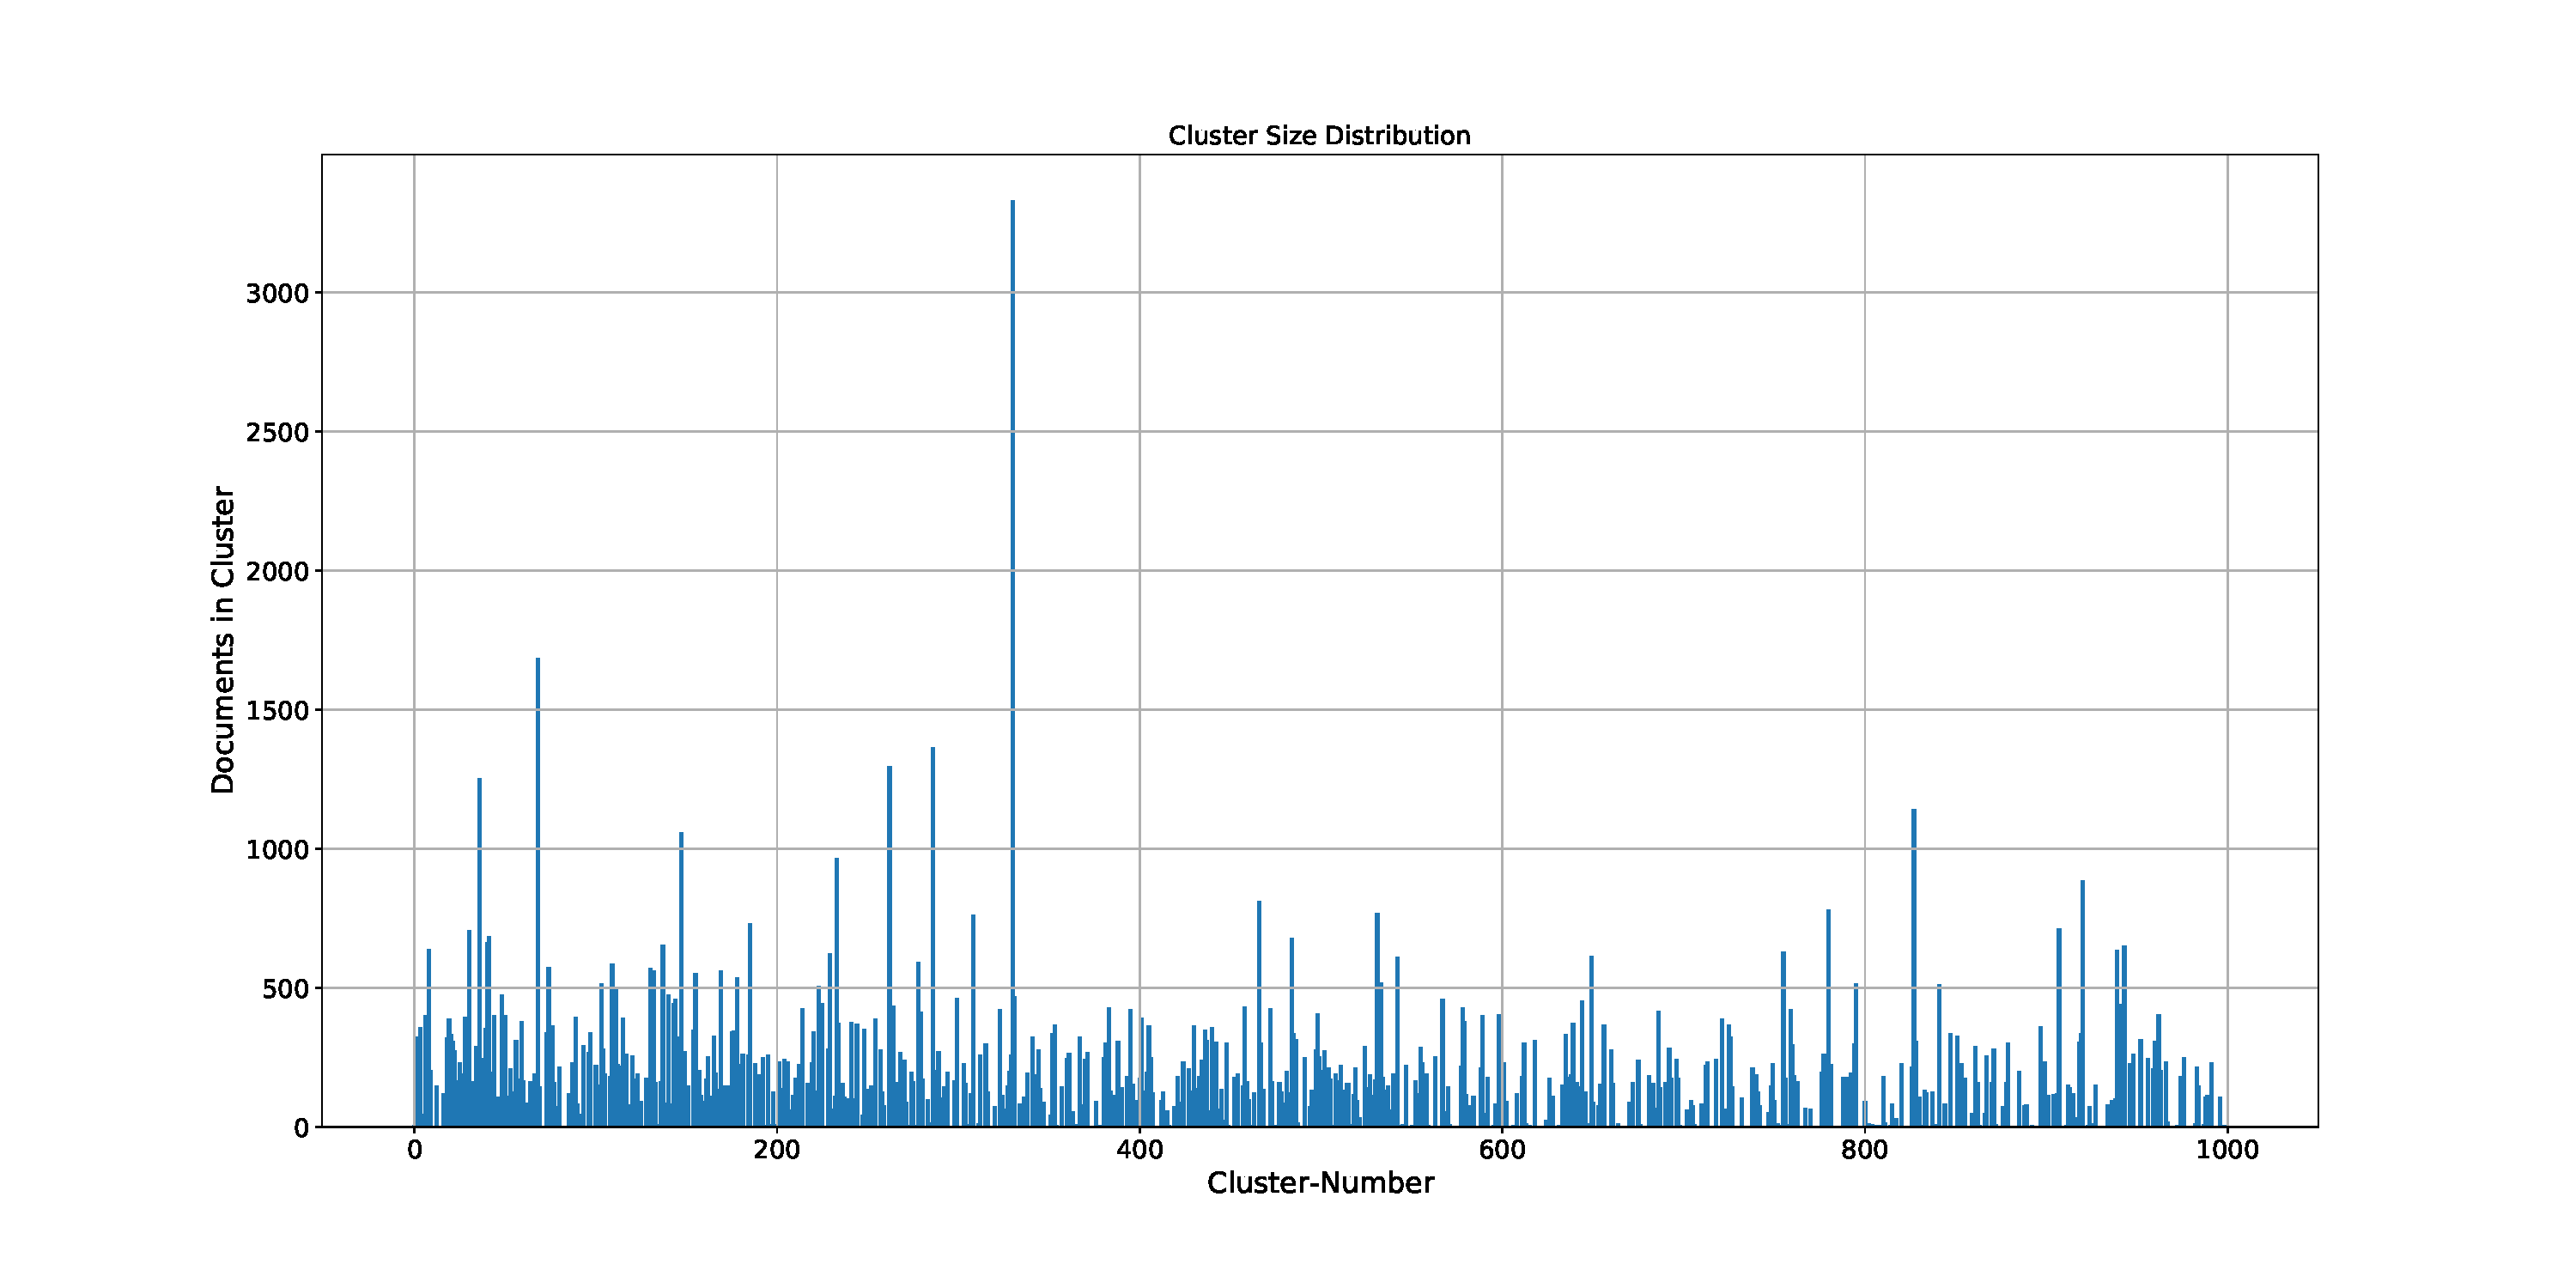
\includegraphics[width=1.0\textwidth]{Graphs/cluster_size_dist.pdf}
 \caption{Cluster Size Distribution}
\end{figure}
\end{flushleft}
\subsection{GLOVE}
\subsection{BERT}

\newpage
\section{Baseline 1: How Topic Similarity affects Model Performance}
\begin{flushleft}
Here we want to measure how well a recommendation system performs on an unseen topic for users with different types of preferences and how this performance varies as similarity between topics increases (seen and unseen topic similarity).
\end{flushleft}
\subsection{TF-IDF}
\vspace{-5ex}
\begin{figure}[H]
 \centering
 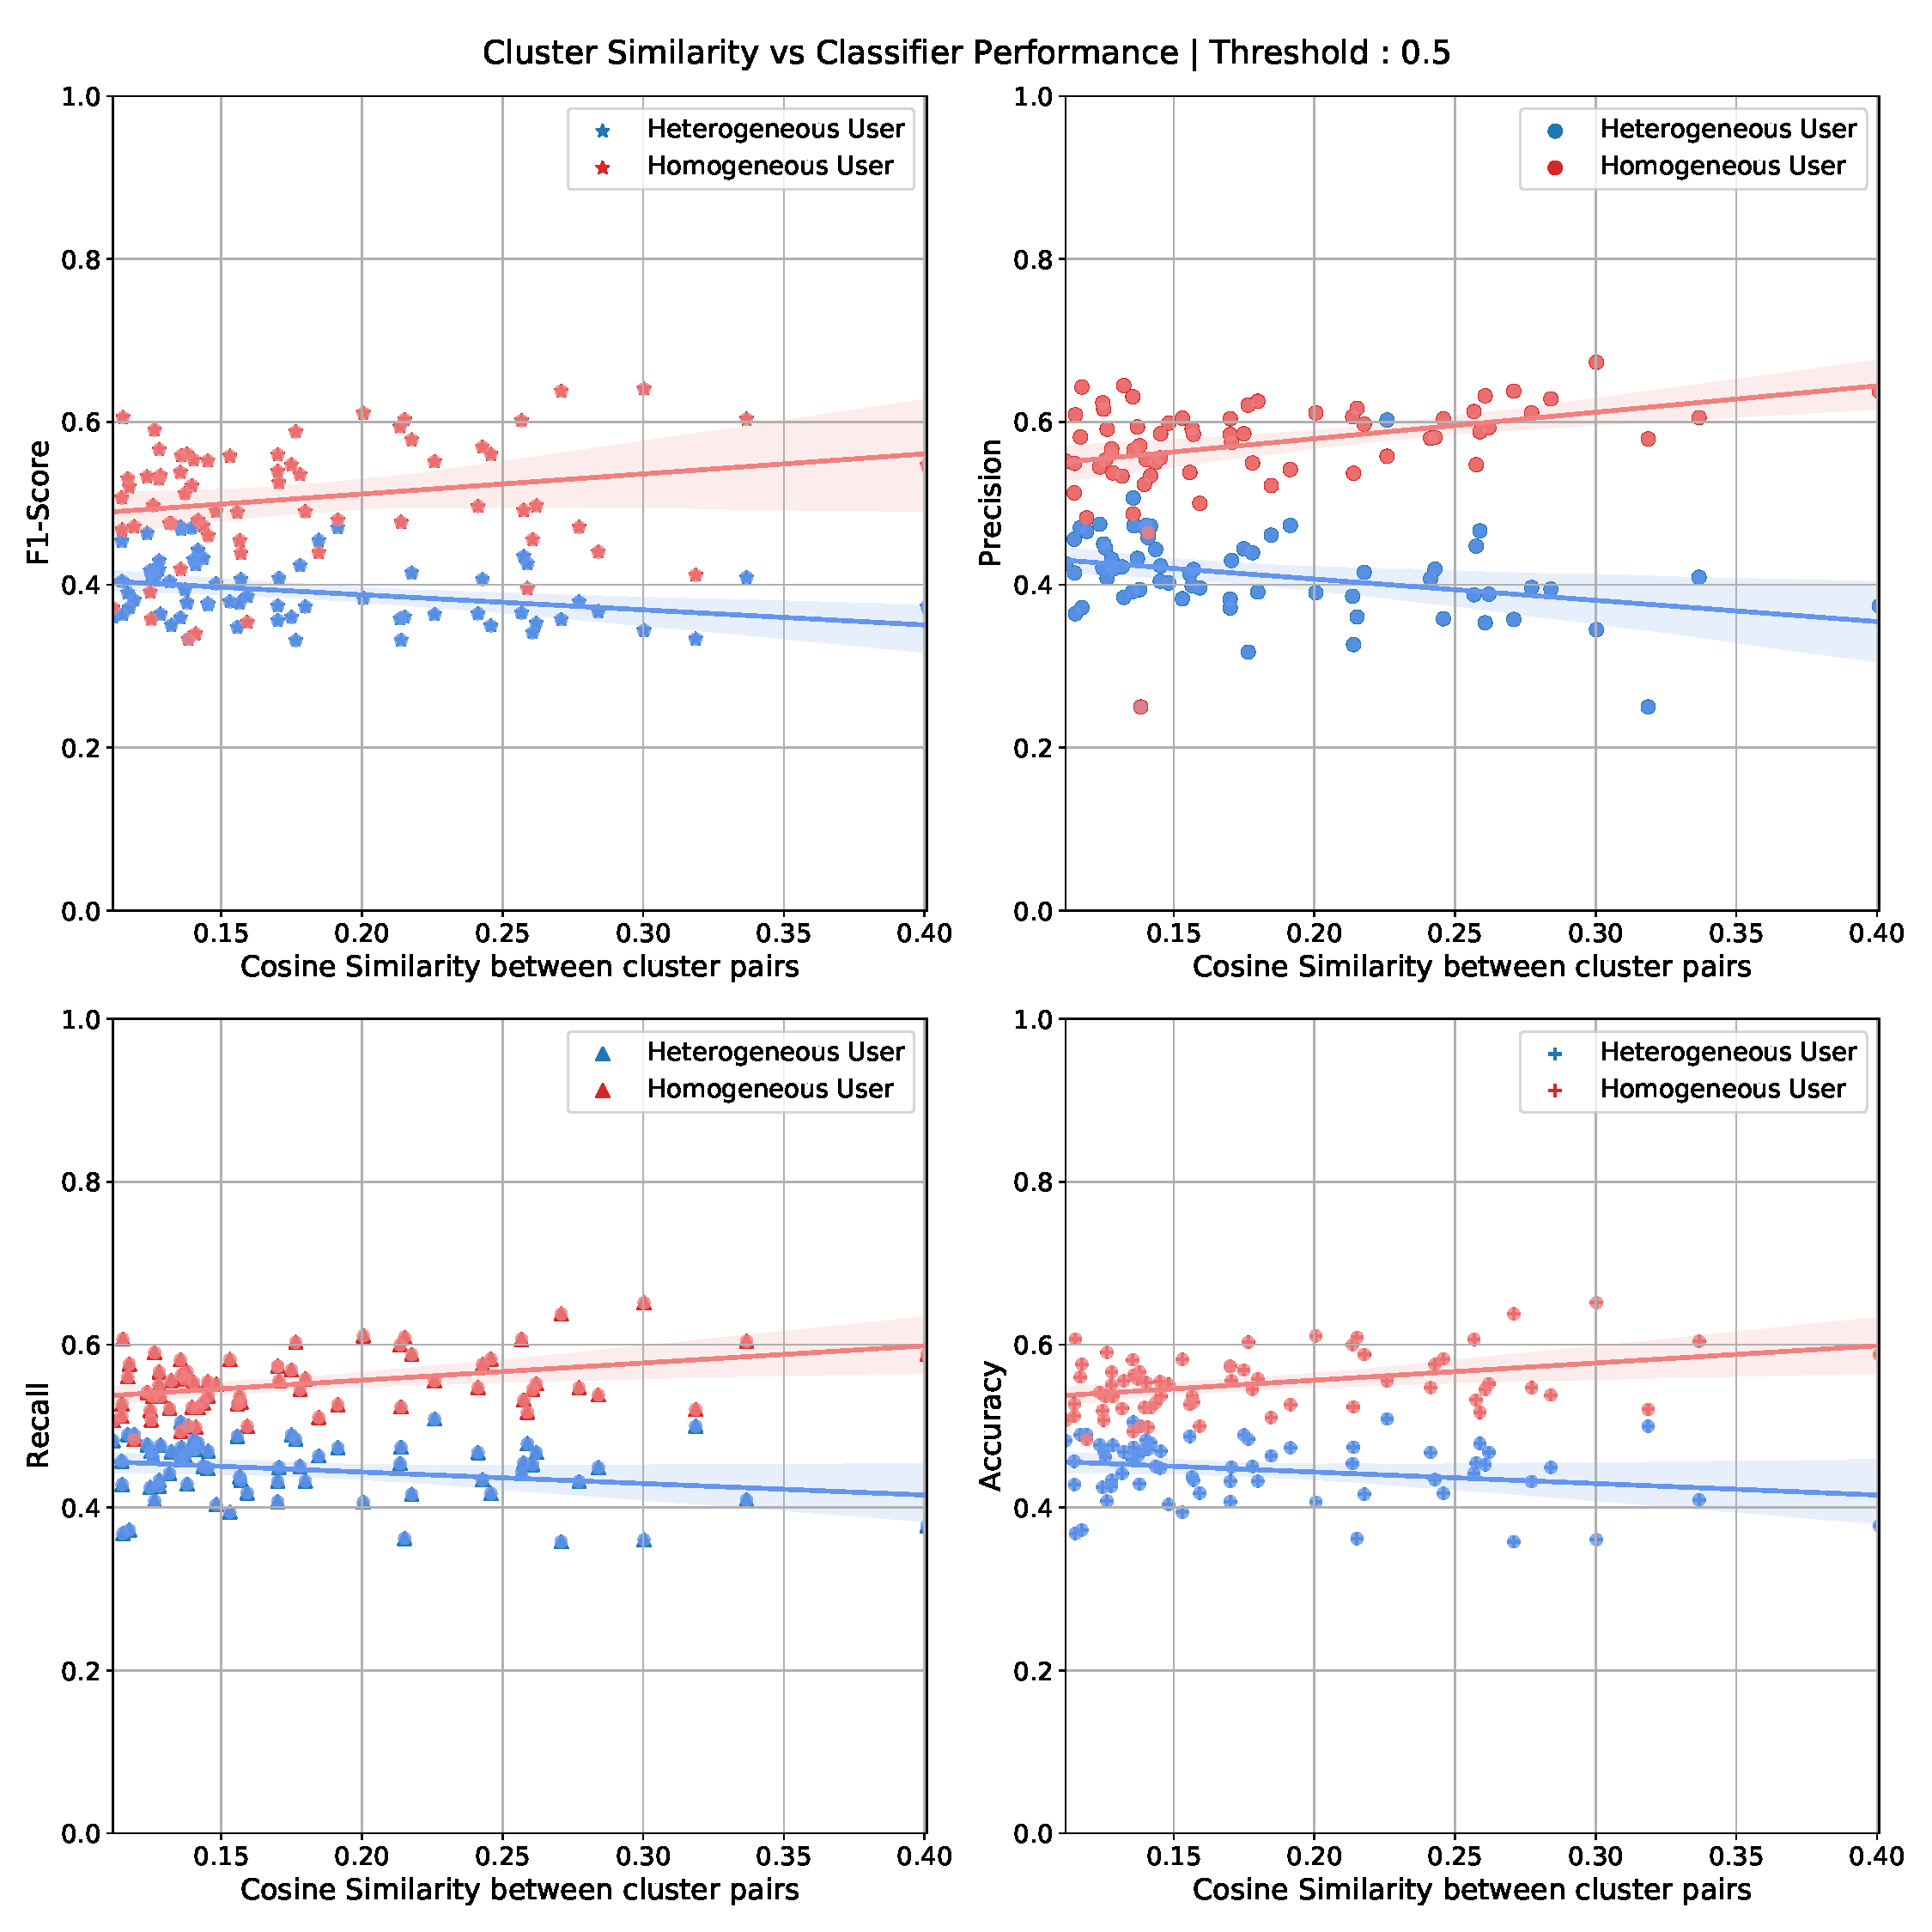
\includegraphics[width=0.8\textwidth]{Graphs/TFIDF/cluster_sim_vs_model_perf_5.pdf}
 \caption{\textbf{Cosine Similarity between Cluster/Topic Pairs vs F1, Precision, Recall and Accuracy.The models are trained on cluster 1 and metrics are measured on cluster 2 which is used as a test set} - TFIDF}
\end{figure}
\begin{flushleft}
\textbf{Note :} The metrics measured for this baseline experiment is based on a test set and not calculated at a particular time step or user-interaction
\begin{itemize}
    \item We see that for homogeneous user's there is an increase in \textbf{Precision} and \textbf{Recall} when similarity between the clusters/topics increases.
    \item For a Heterogeneous User we see the opposite effect with a decrease in both \textbf{Precision} and \textbf{Recall} as similarity between cluster pairs increases (hence harder for the classifier to distinguish between positives from cluster 1 and negatives from cluster 2 when both are more similar).
\end{itemize}
\end{flushleft}
\subsection{Glove}
\vspace{-5ex}
\begin{figure}[H]
 \centering
 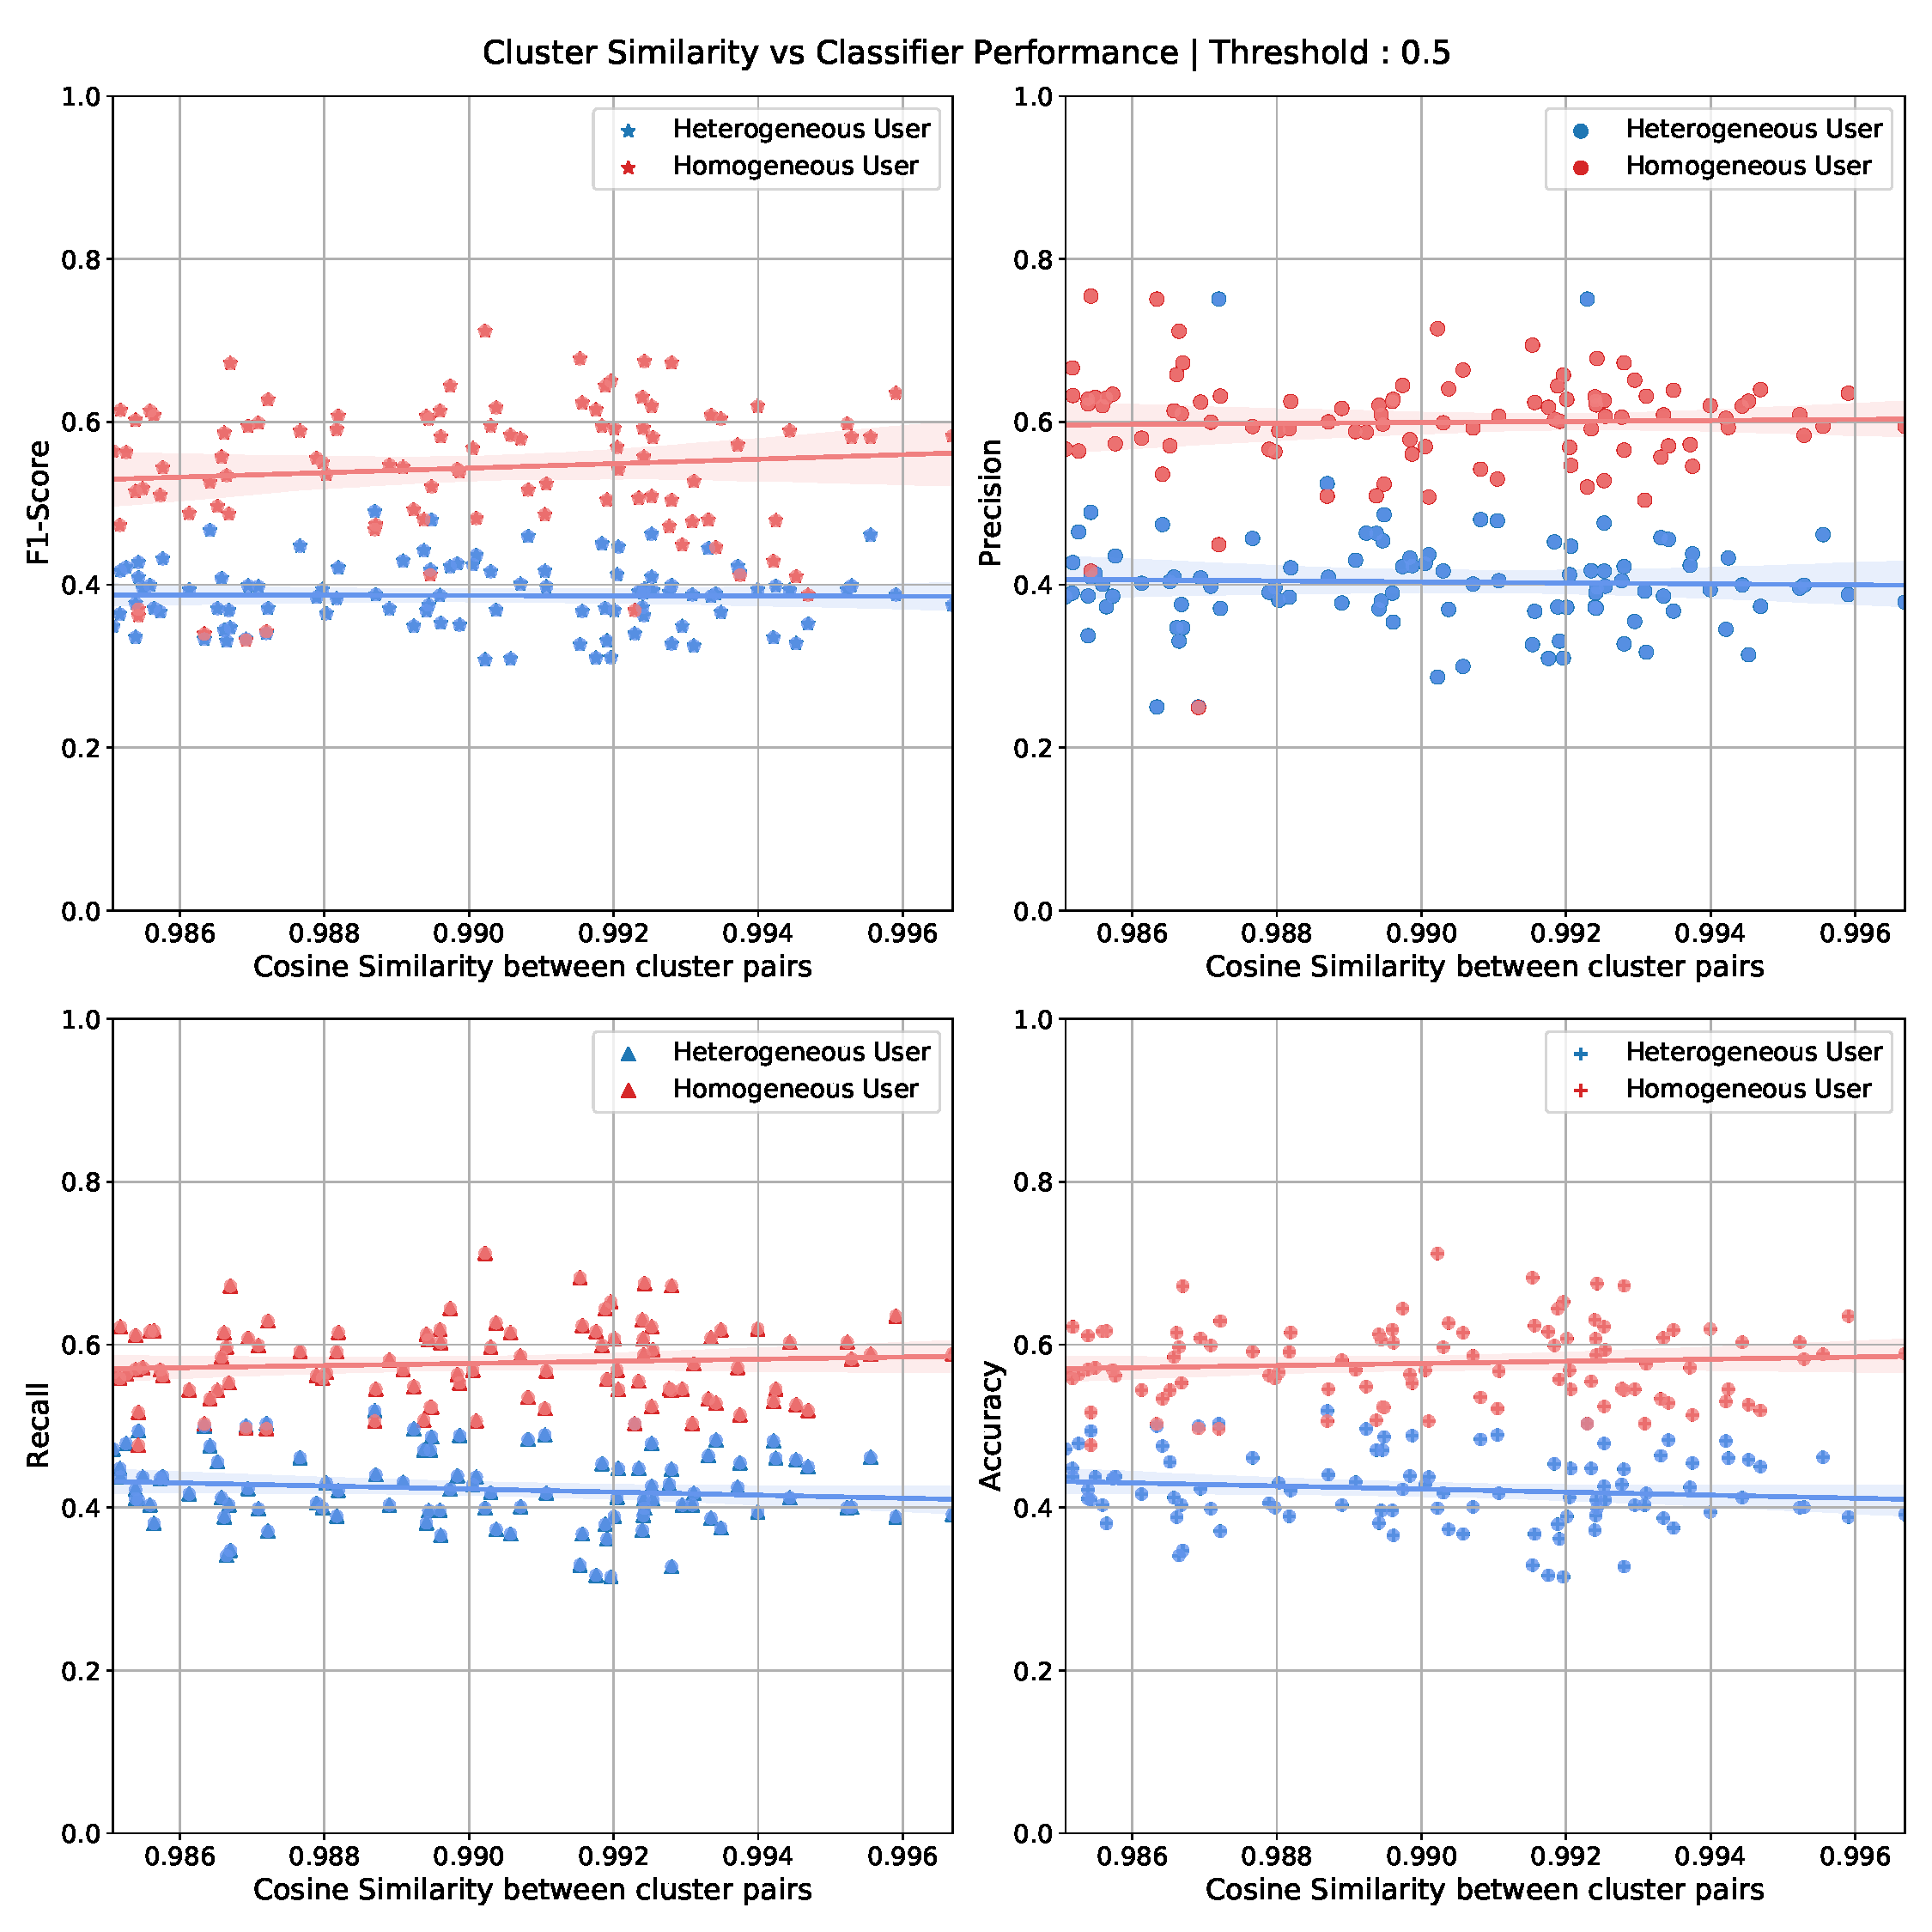
\includegraphics[width=0.8\textwidth]{Graphs/GLOVE/cluster_sim_vs_model_perf_5.pdf}
 \caption{\textbf{Cosine Similarity between Cluster/Topic Pairs vs F1, Precision, Recall and Accuracy.The models are trained on cluster 1 and metrics are measured on cluster 2 which is used as a test set} - GLOVE}
\end{figure}
\begin{flushleft}
\begin{itemize}
    \item We see that for homogeneous user's there is an increase in \textbf{Precision} and \textbf{Recall} when similarity between the clusters/topics increases (only slight increase occurs here as the cluster pairs seem be more similar here compared to clustering using TFIDF).
    \item For a Heterogeneous User we see the opposite effect with a decrease in both \textbf{Precision} and \textbf{Recall} as similarity between cluster pairs increases (but smaller decrease compared to using TFIDF).
\end{itemize}
\end{flushleft}
\subsection{BERT}
\vspace{-5ex}
\begin{figure}[H]
 \centering
 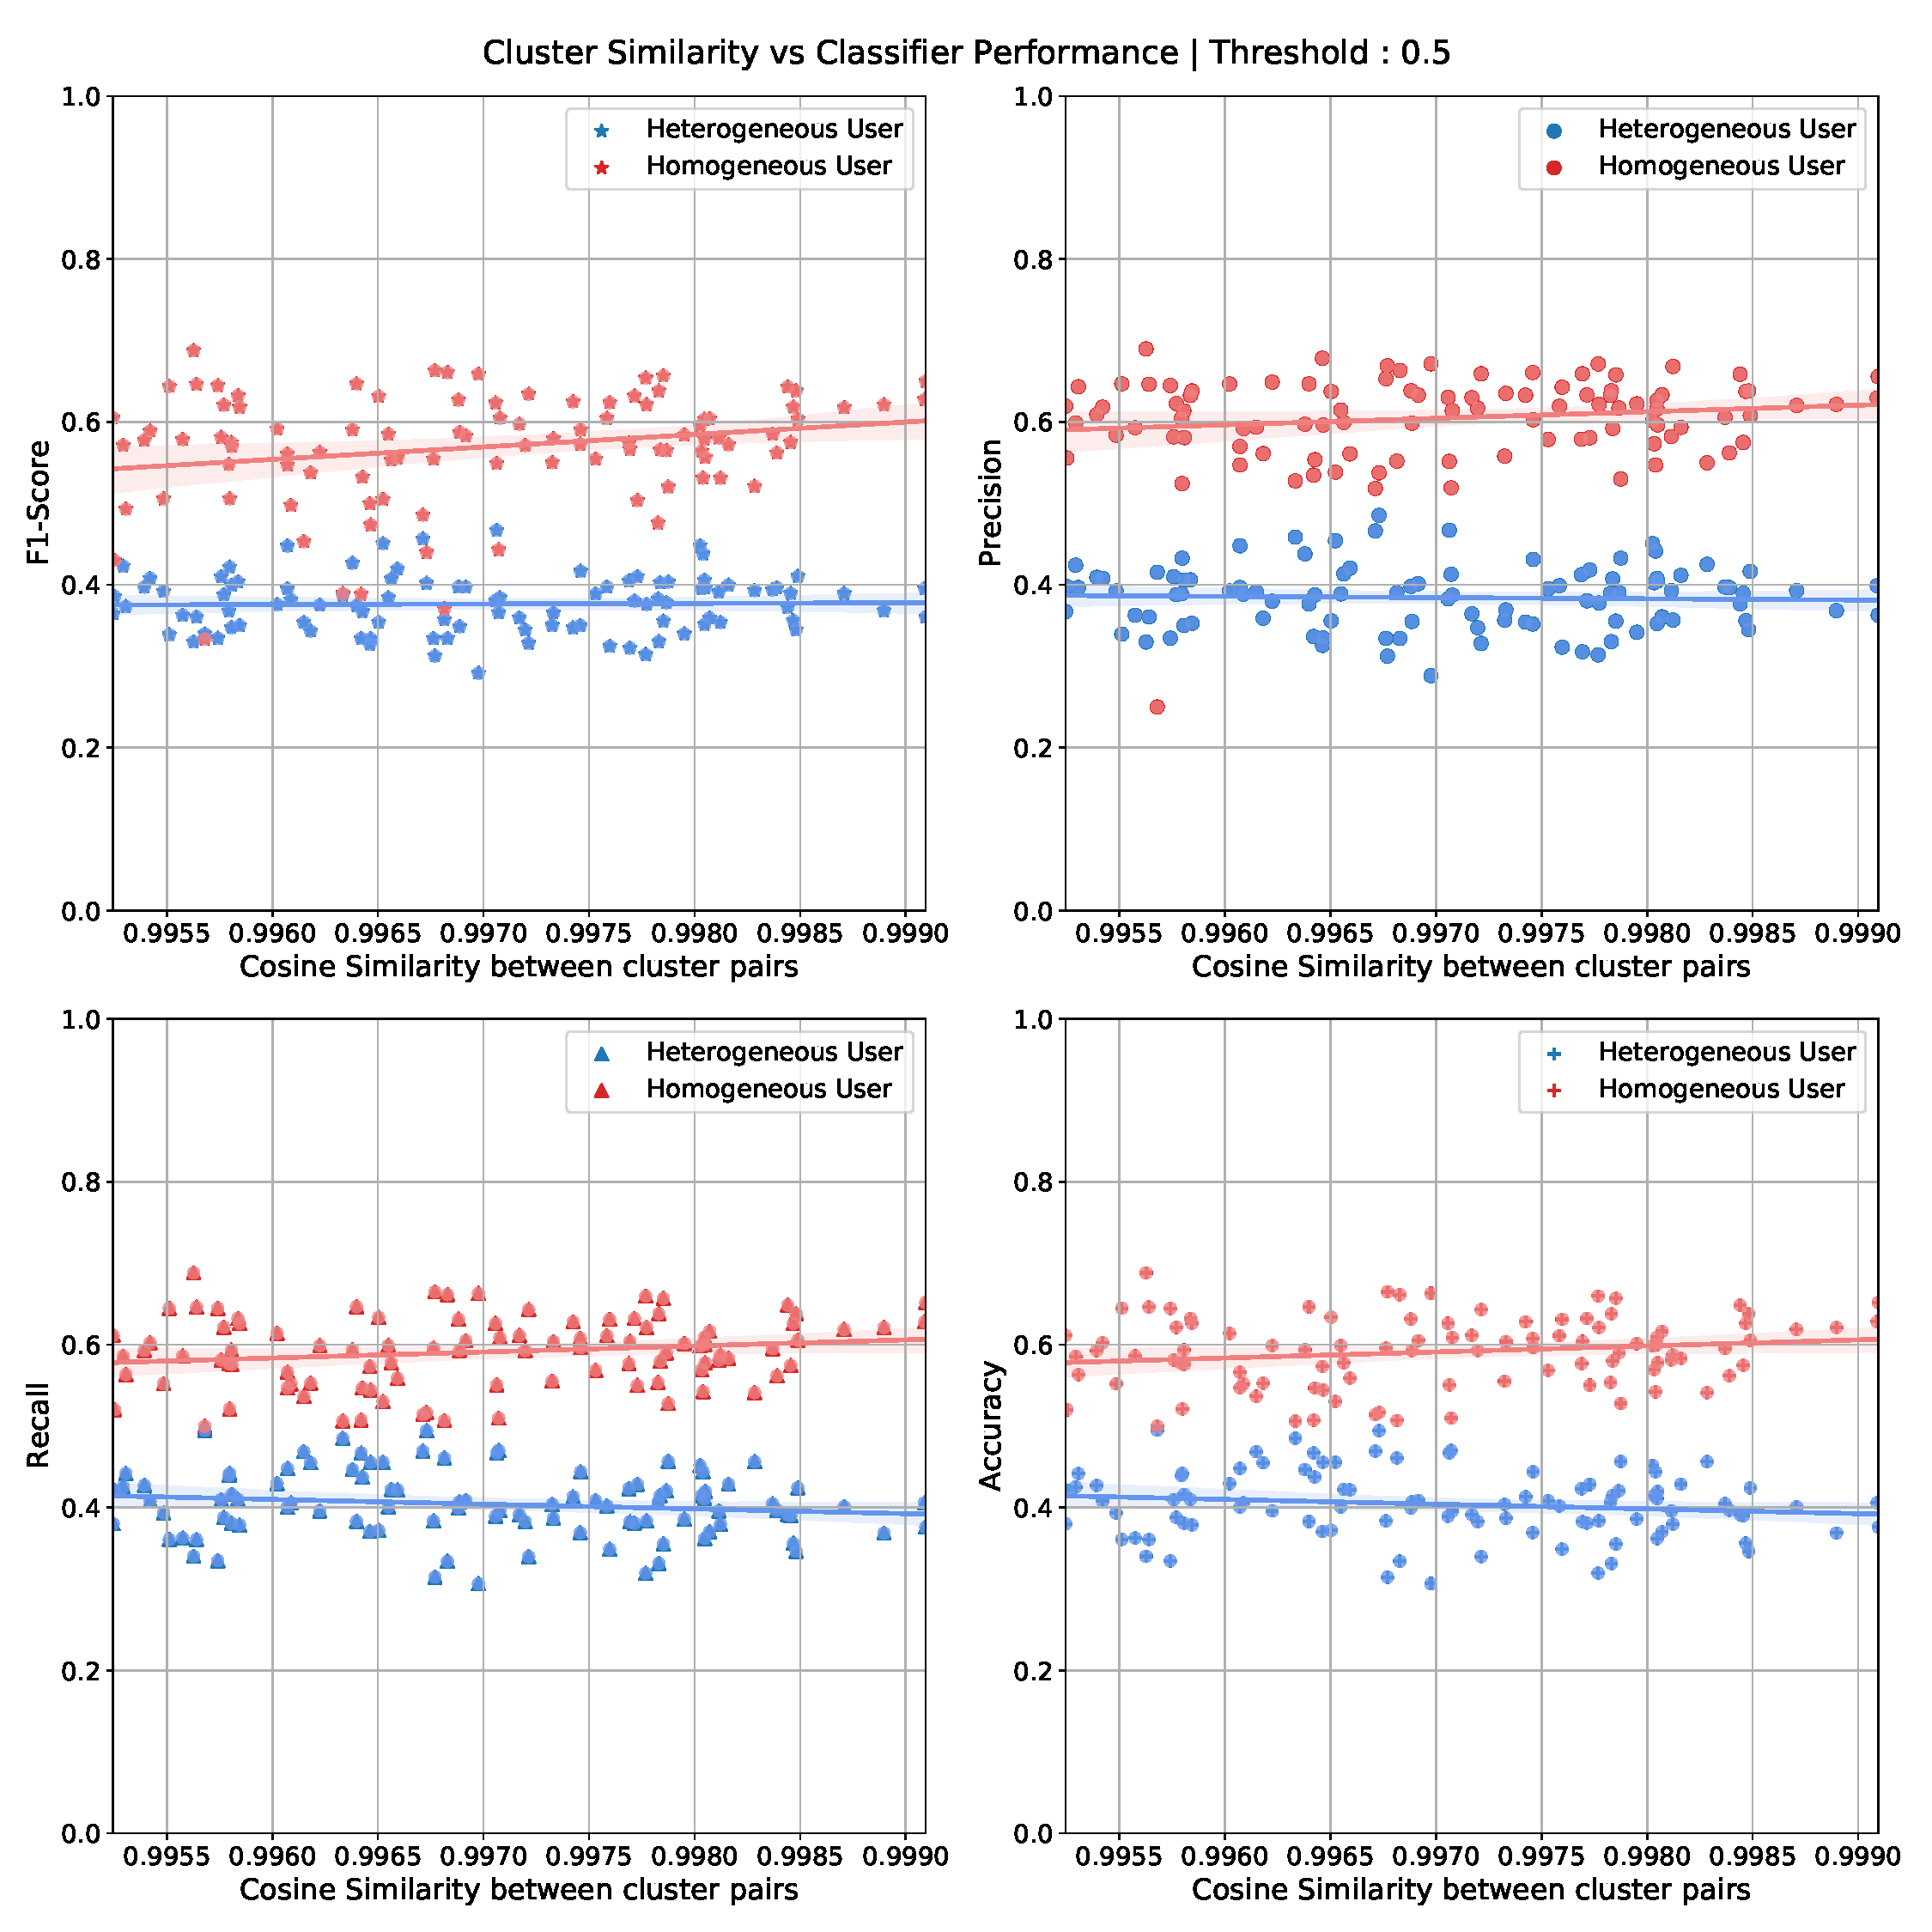
\includegraphics[width=0.8\textwidth]{Graphs/BERT/cluster_sim_vs_model_perf_5.pdf}
 \caption{\textbf{Cosine Similarity between Cluster/Topic Pairs vs F1, Precision, Recall and Accuracy.The models are trained on cluster 1 and metrics are measured on cluster 2 which is used as a test set} - BERT}
\end{figure}
\begin{flushleft}
\begin{itemize}
    \item Similar Performance like GLOVE but the clustering of pairs is even better now as we choose extremely similar cluster pairs measured according to cosine similarity.
\end{itemize}
\end{flushleft}


\vspace{-1ex}
\section{Baseline 2: Online Learning Setting}
\begin{flushleft}
To emulate a real-world scenario , we want to simulate a recommendation system interacting with a user over a set of unseen articles , slowly updating itself to learn the user's preferences over time, \textbf{N=200} is used here to calculate the metrics, where \textbf{N }represents the number of interactions between the user and the content recommender. Also to note, there are at least N relevant articles in the candidate pool. 
\end{flushleft}
\begin{flushleft}
For this baseline experiment we use recommender specific metrics such as \textbf{Precision@K} and \textbf{Recall@K}.
\begin{itemize}
    \item $Precision@K = \frac{\# recommended \; items \: the \: user \; likes \: at \: K_{th} \: Interaction}{total \: \#  \: of \: items \:  recommended \: at \: K_{th} \: Interaction}$
    
    \item $Recall@K = \frac{\# recommended \; items \: the \: user \; likes \: at \: K_{th} \; Interaction}{total \; \# of \; relevant \; items \; in \; the \; candidate \; pool}$
    
    \item Eg:  \begin{itemize}
        \item Candidate Pool Size = 15
        \item Number of relevant(user-likes) items in the candidate pool = 10
        \item N = 1 \begin{itemize}
            \item Shown Articles = [0]
            \item Recall = 0/10 = 0
            \item Precision = 0/1 = 0
        \end{itemize}
        \item N = 2 \begin{itemize}
            \item Shown Articles = [0,1]
            \item Recall = 1/10 = 0.1
            \item Precision = 1/2 = 0.5
        \end{itemize}
        \item N = 3 \begin{itemize}
            \item Shown Articles = [0,1,1]
            \item Recall = 2/10 = 0.2
            \item Precision = 2/3 = 0.666
        \end{itemize}
        \item N = 4 \begin{itemize}
            \item Shown Articles = [0,1,1,1]
            \item Recall = 3/10 = 0.3
            \item Precision = 3/4 = 0.75
        \end{itemize}
    \end{itemize}
    
\end{itemize}
\end{flushleft}
\subsection{TF-IDF}
\vspace{1ex}
\begin{figure}[H]
 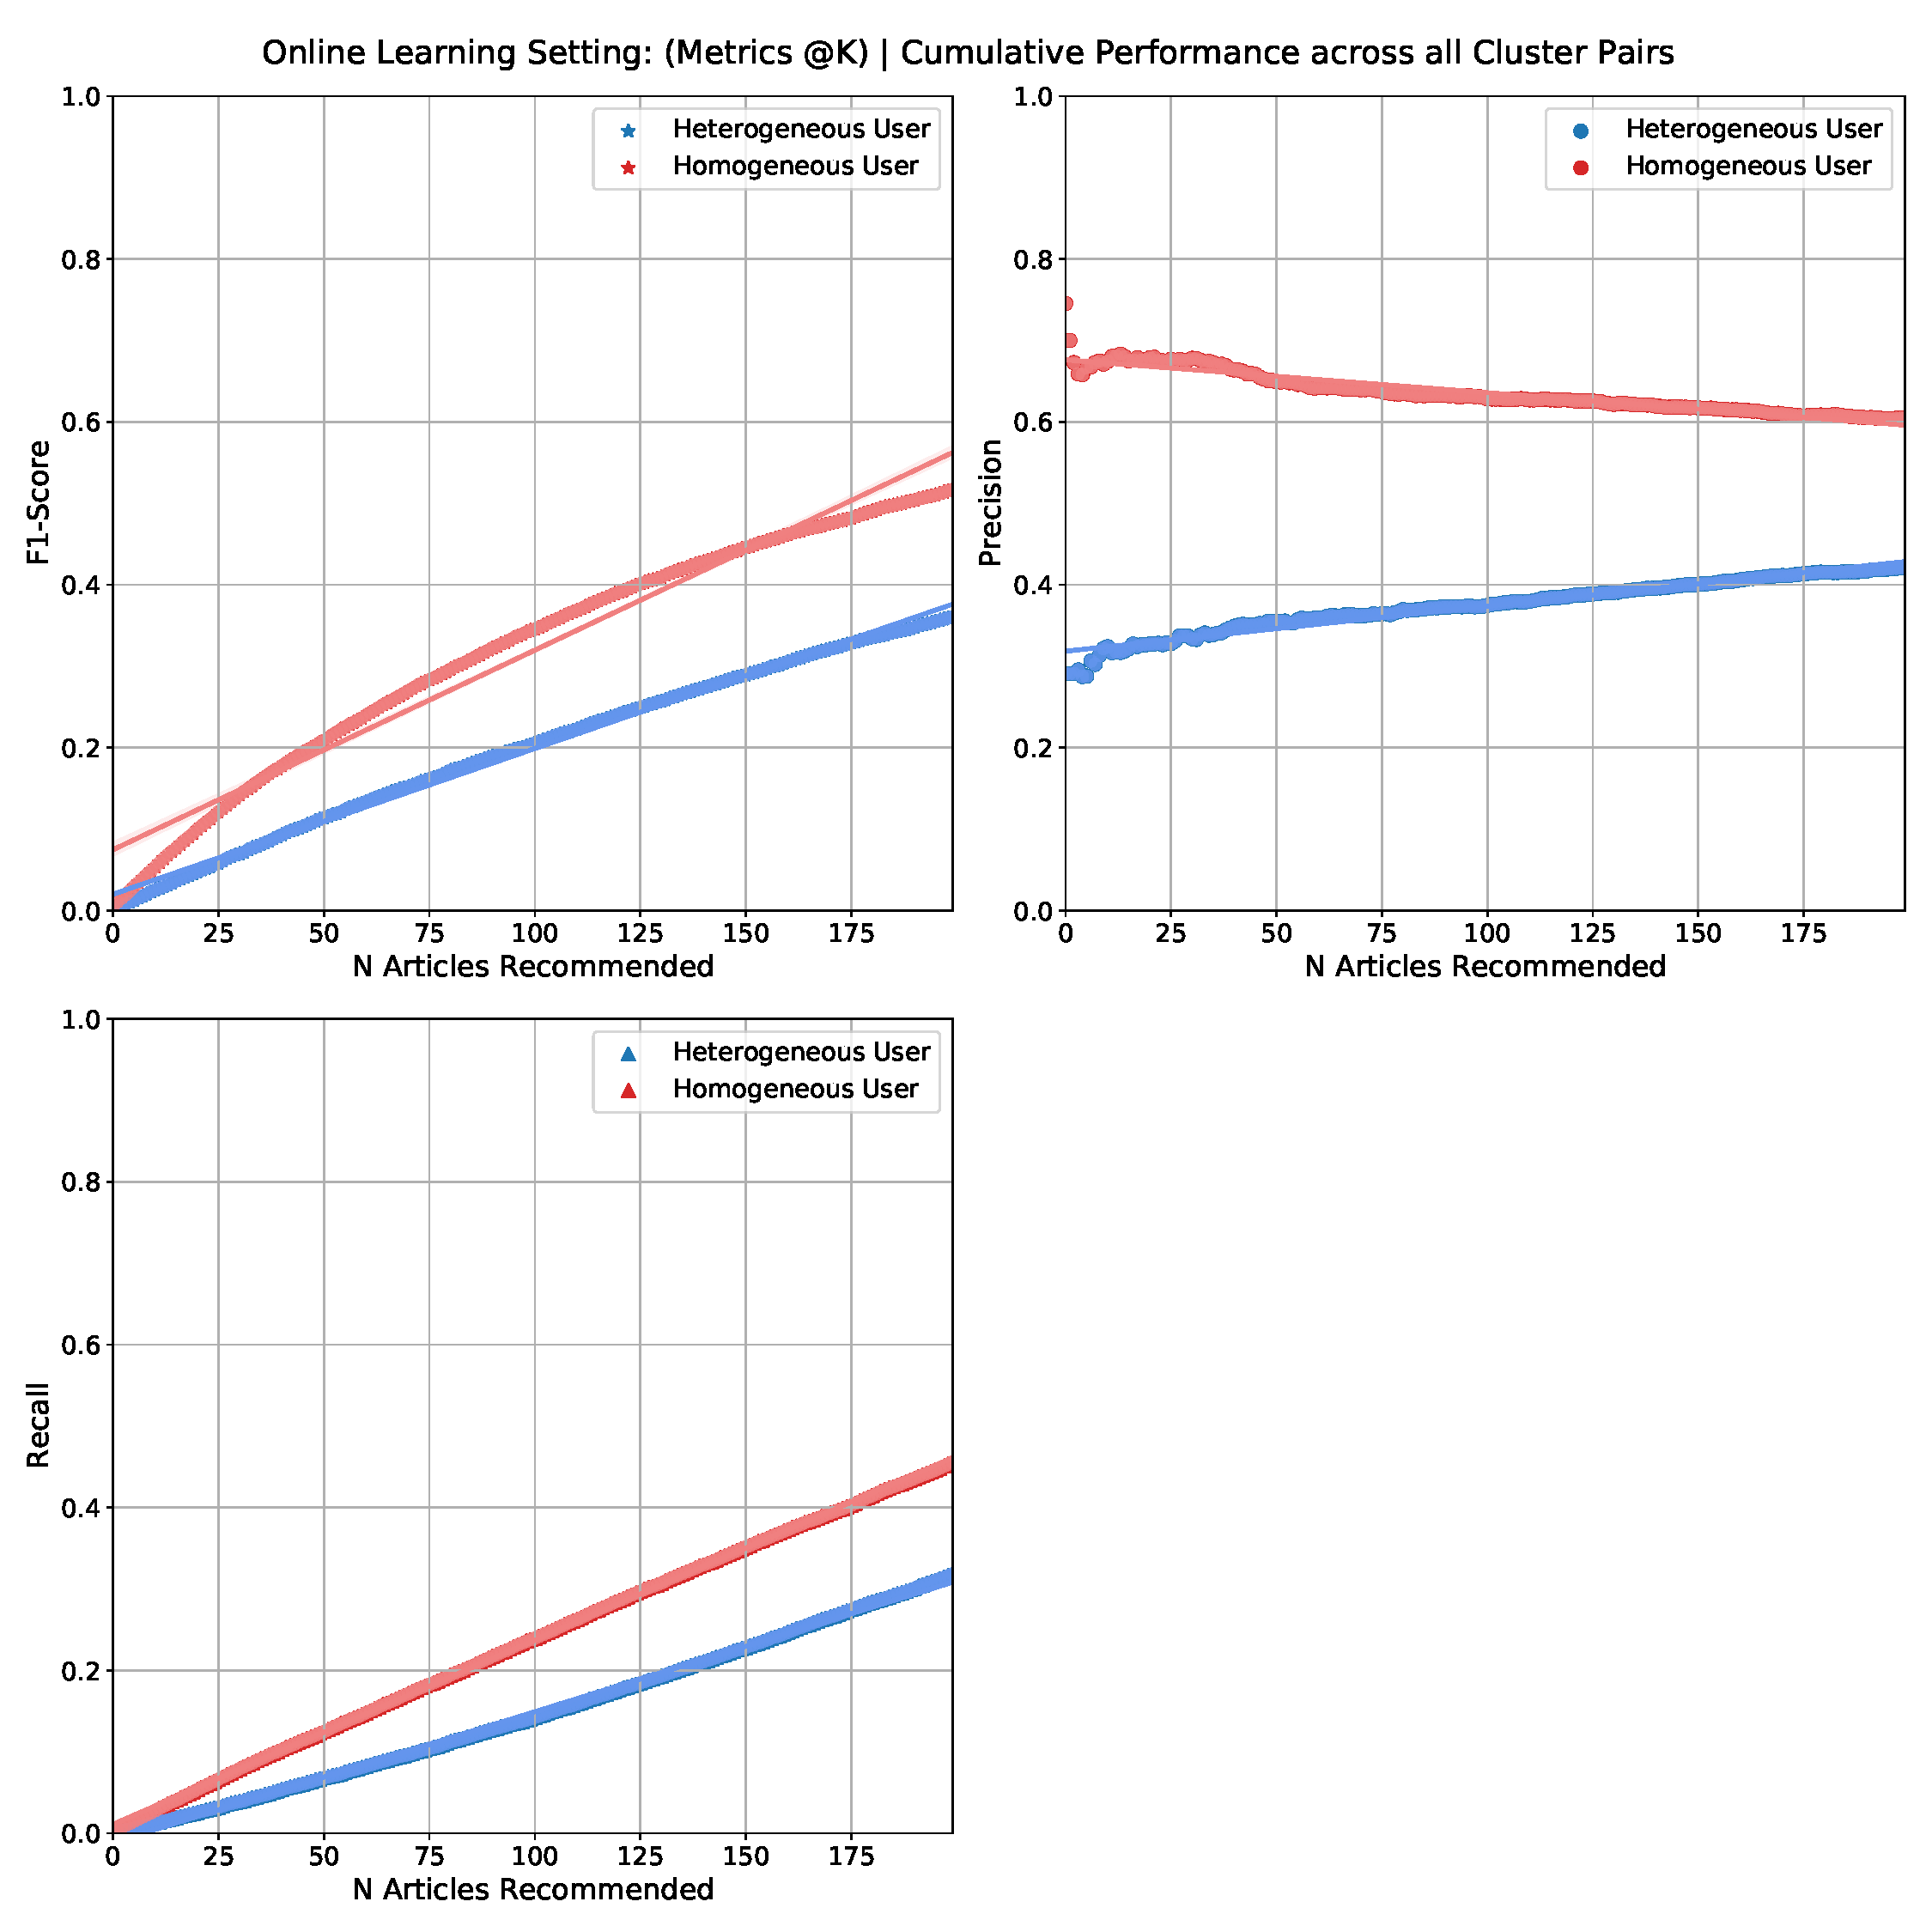
\includegraphics[width=0.8\textwidth]{Graphs/TFIDF/user_interaction_vs_model_performance_cumu.pdf}
\end{figure}
\vspace{-4ex}
\begin{figure}[H]
 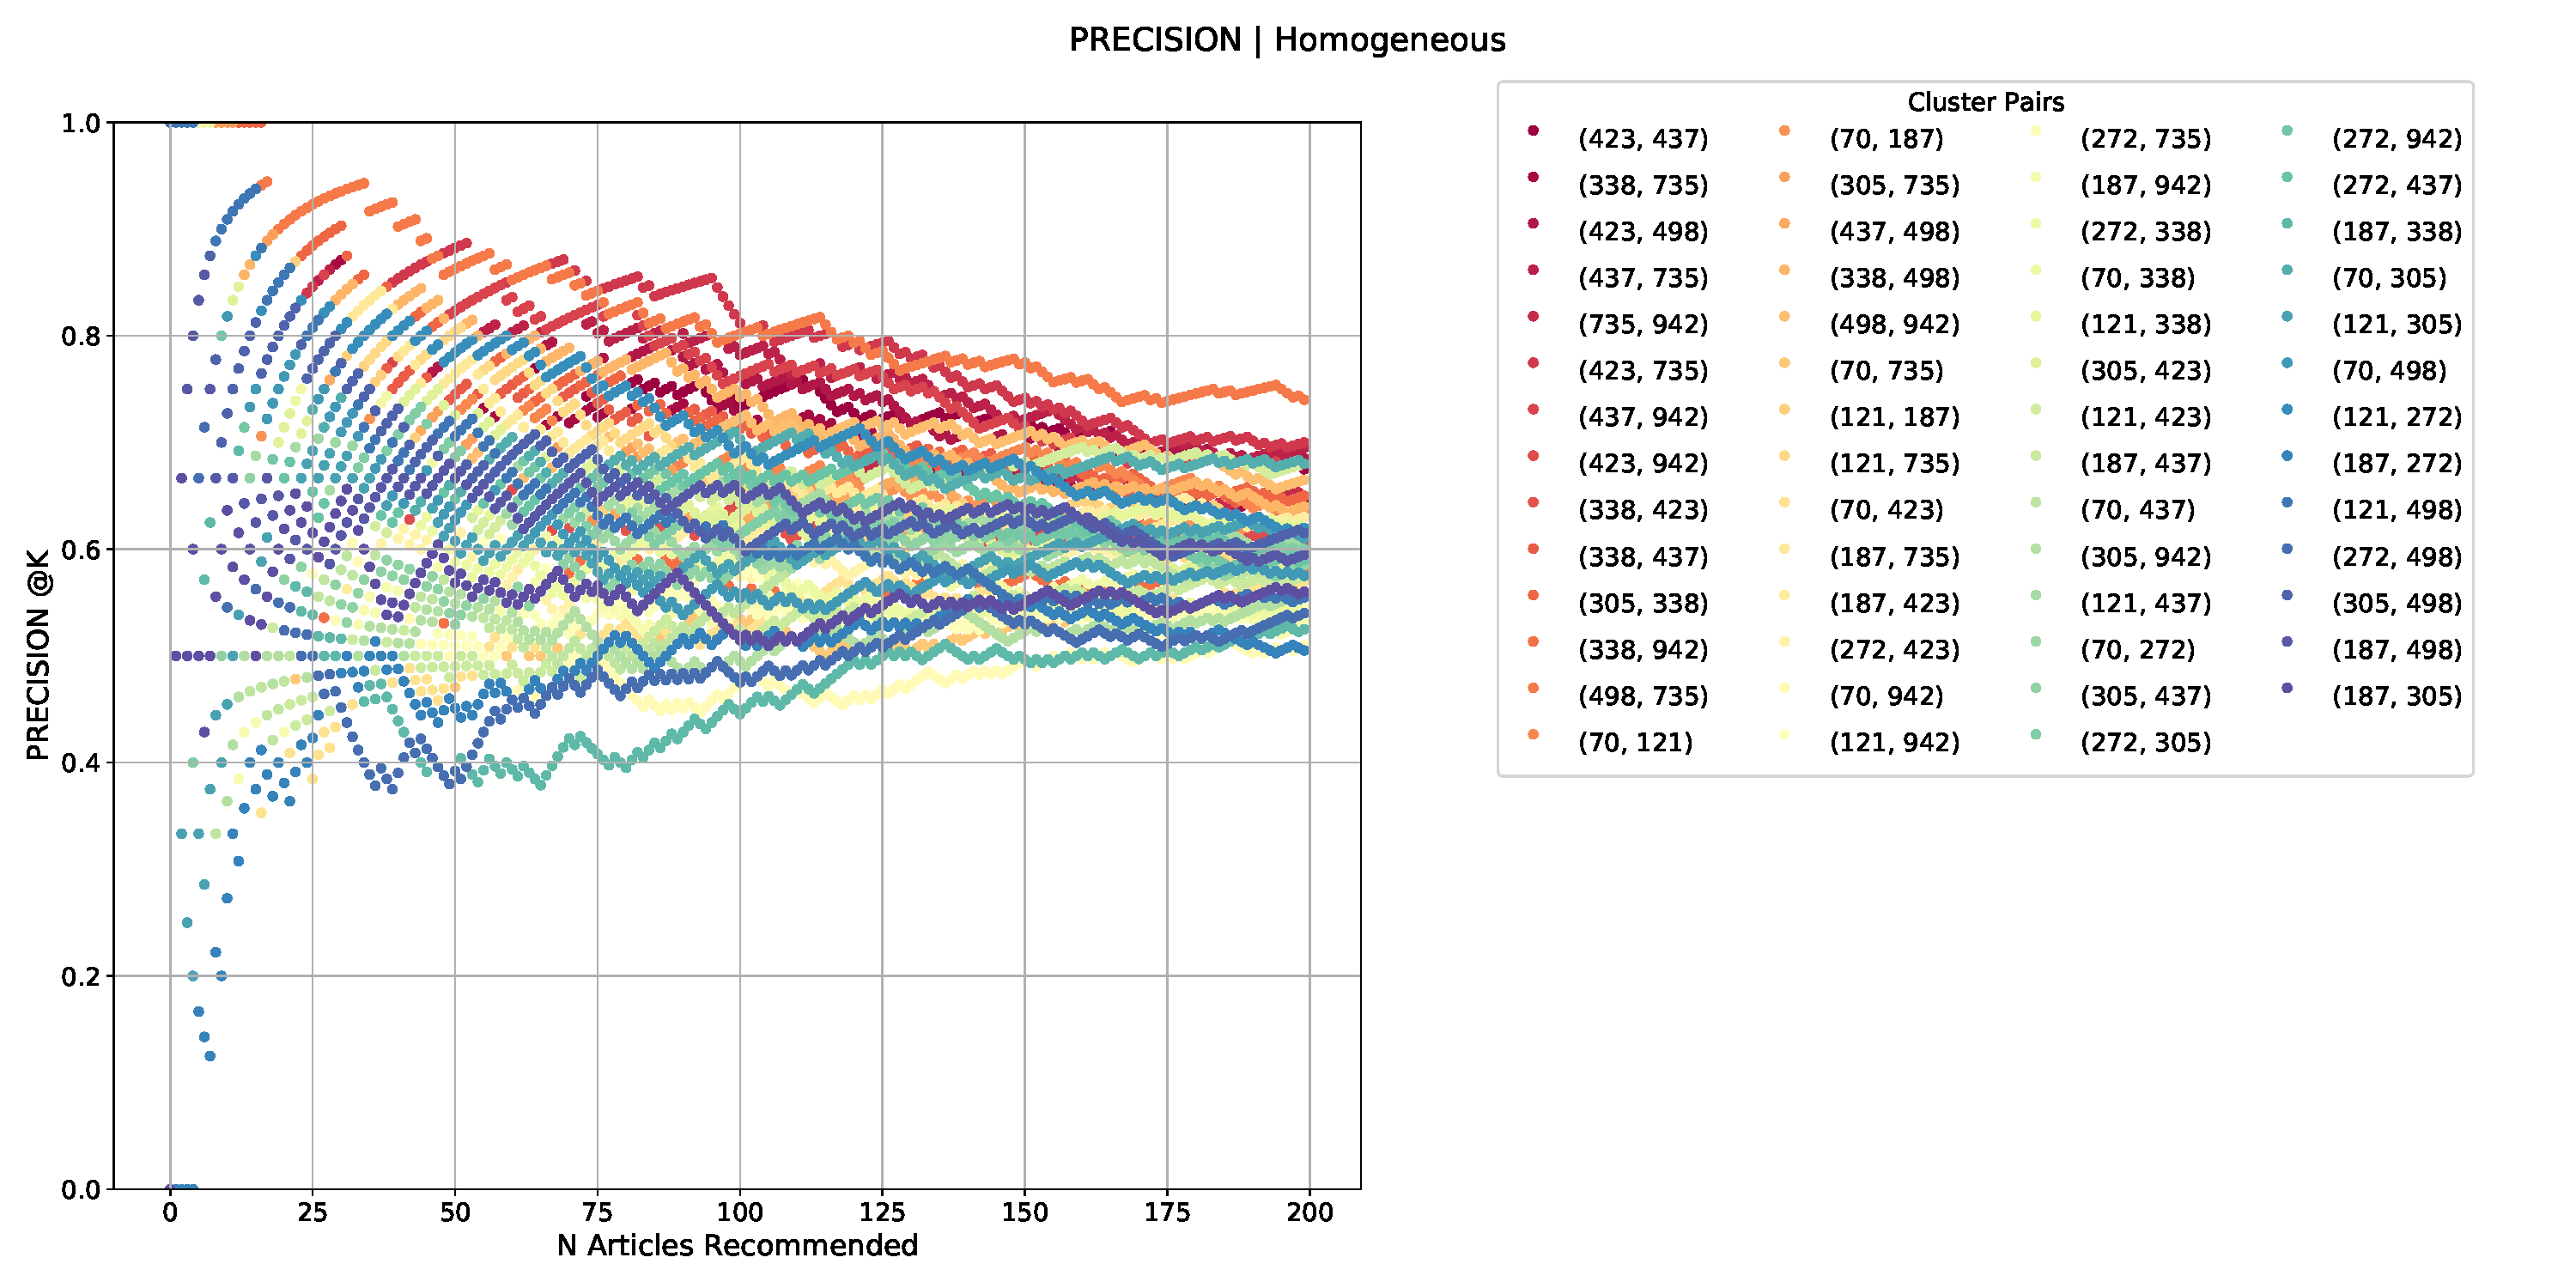
\includegraphics[width=1.0\textwidth]{Graphs/TFIDF/user_interaction_vs_model_performance_precision_all_cps_Homogeneous.pdf}
\end{figure}
\vspace{-1ex}
\begin{figure}[H]
 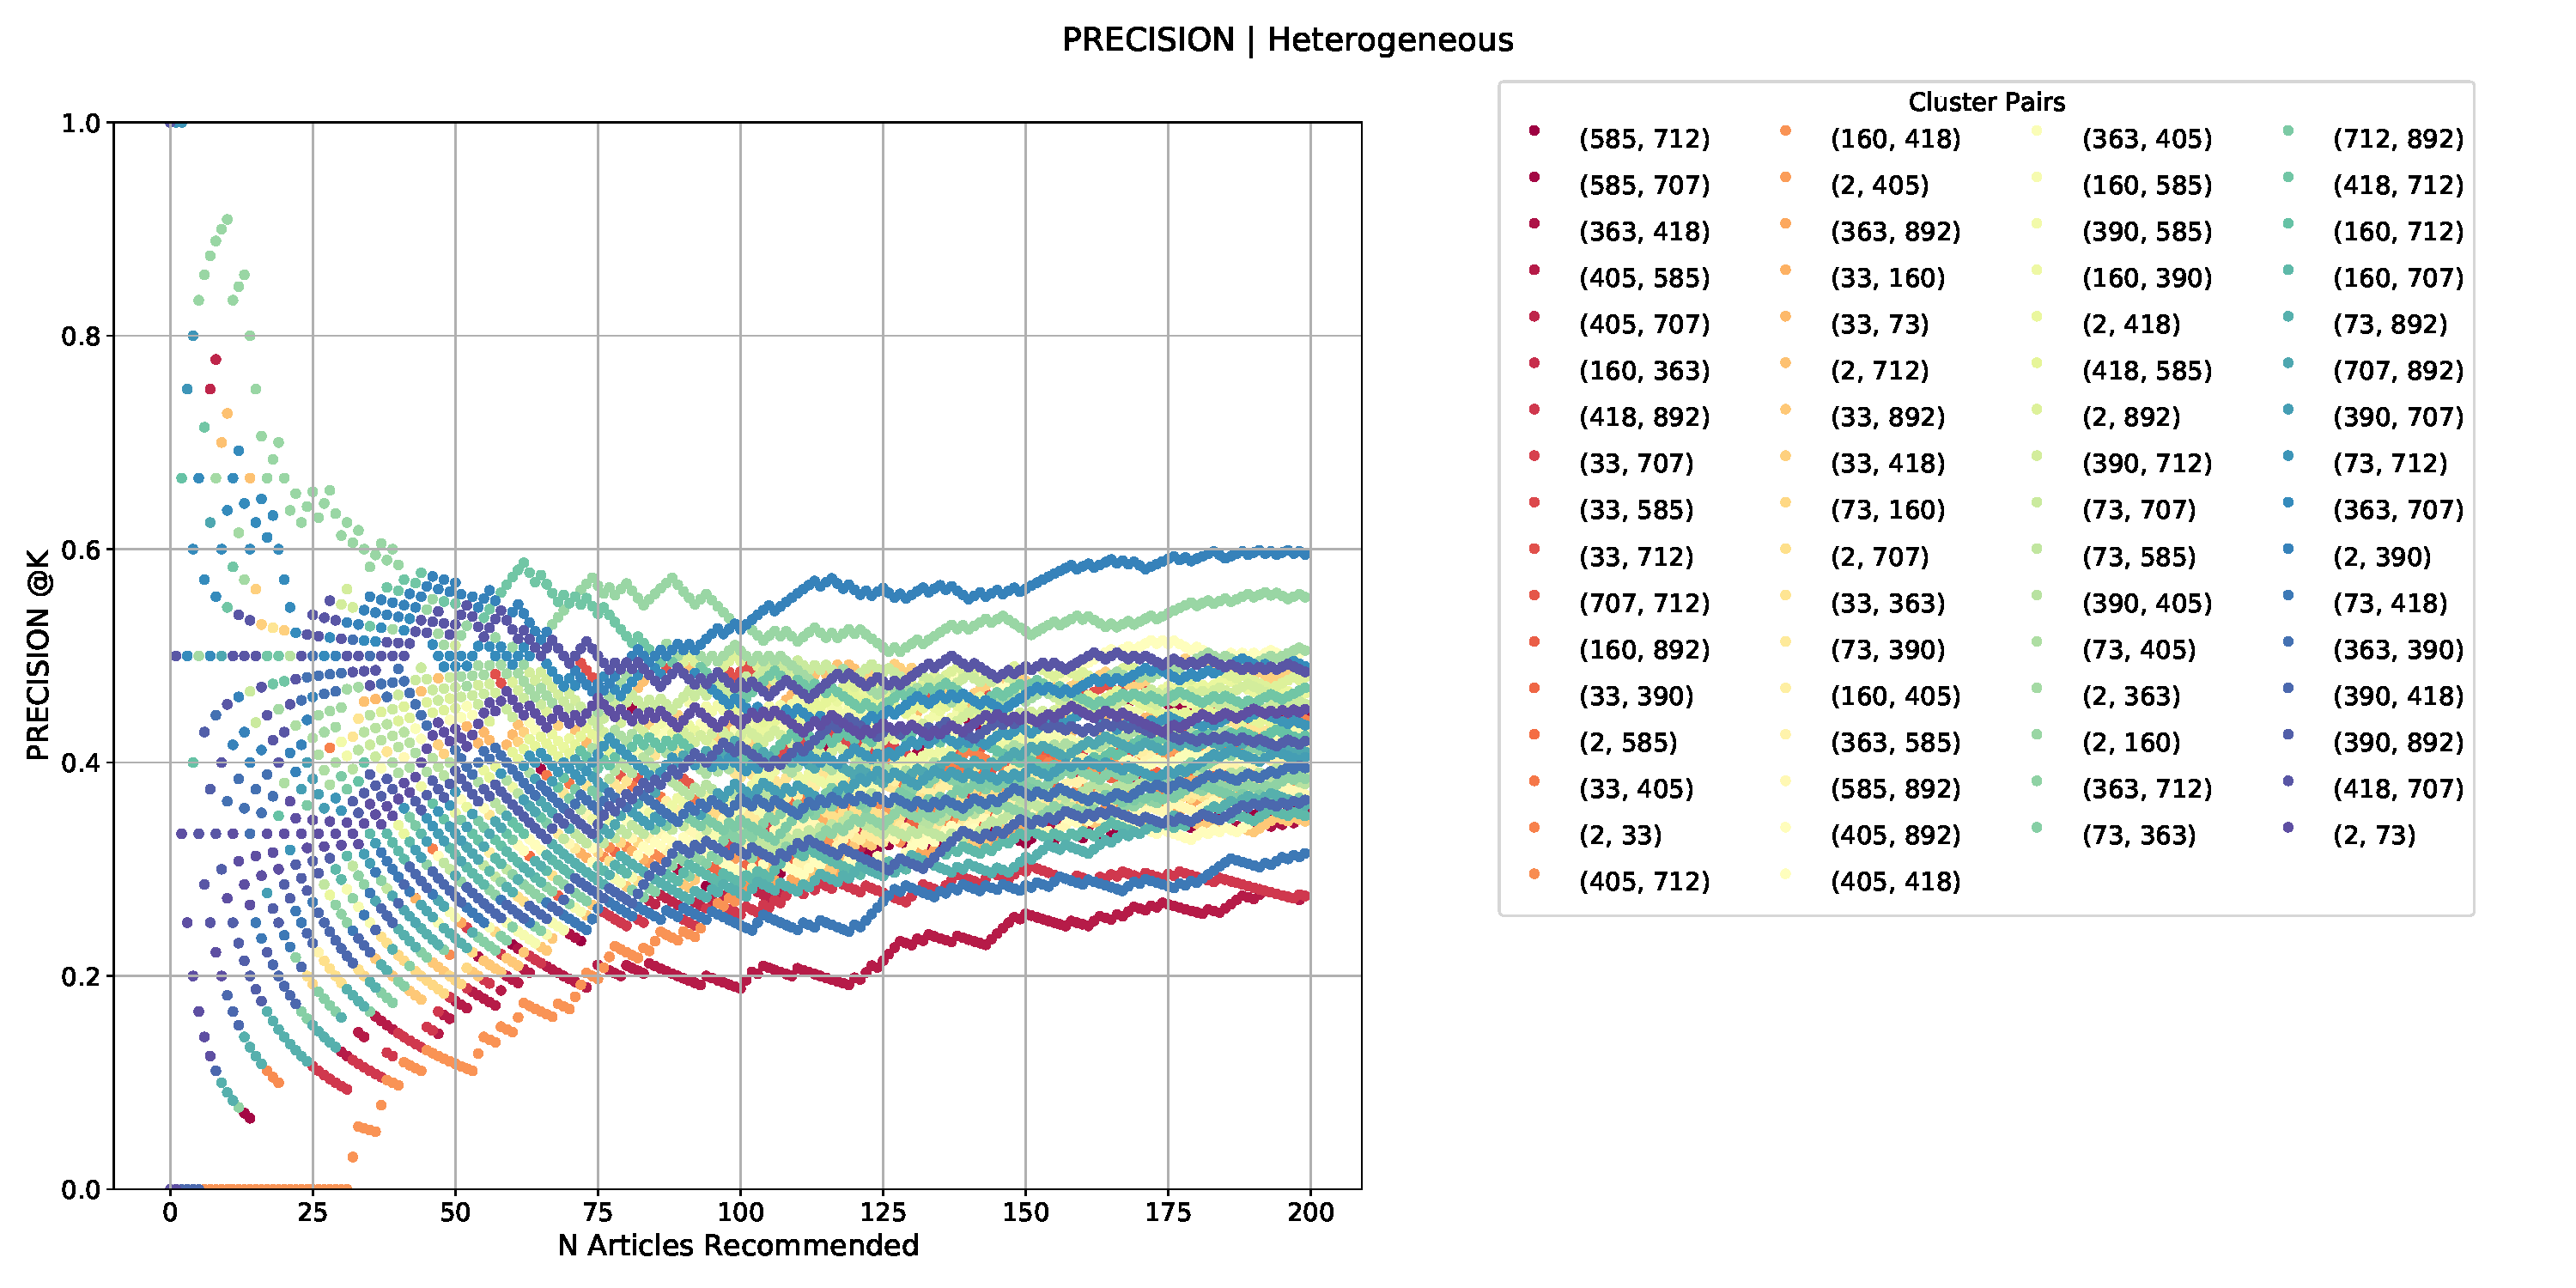
\includegraphics[width=1.0\textwidth]{Graphs/TFIDF/user_interaction_vs_model_performance_precision_all_cps_Heterogeneous.pdf}
\end{figure}
\begin{flushleft}
The above figure shows the mean results across all cluster pairs.
\begin{itemize}
    \item For the Homogeneous User we see that \textbf{Precision@K} decreases as the number of interactions increase, this could be due to the fact that the most probable items the user likes are already recommended in the initial user-interactions (as we sort by predicted probability) and as interactions increase the classifier is only left with items with low confidence to recommend hence increasing mistakes. Also from the precision graph with all cluster pairs shown we see that a few cluster pairs do increase in precision.
    \item For the Heterogeneous User we see that their is an initial dip in \textbf{Precision@K} and then it increases as the content recommender learns the different preferences of the heterogeneous user.
    \item Overall we see that the precision for Homogeneous users is higher than heterogeneous users
\end{itemize}
\end{flushleft}
\vspace{-3ex}
\subsection{Glove}
\vspace{1ex}
\begin{figure}[H]
 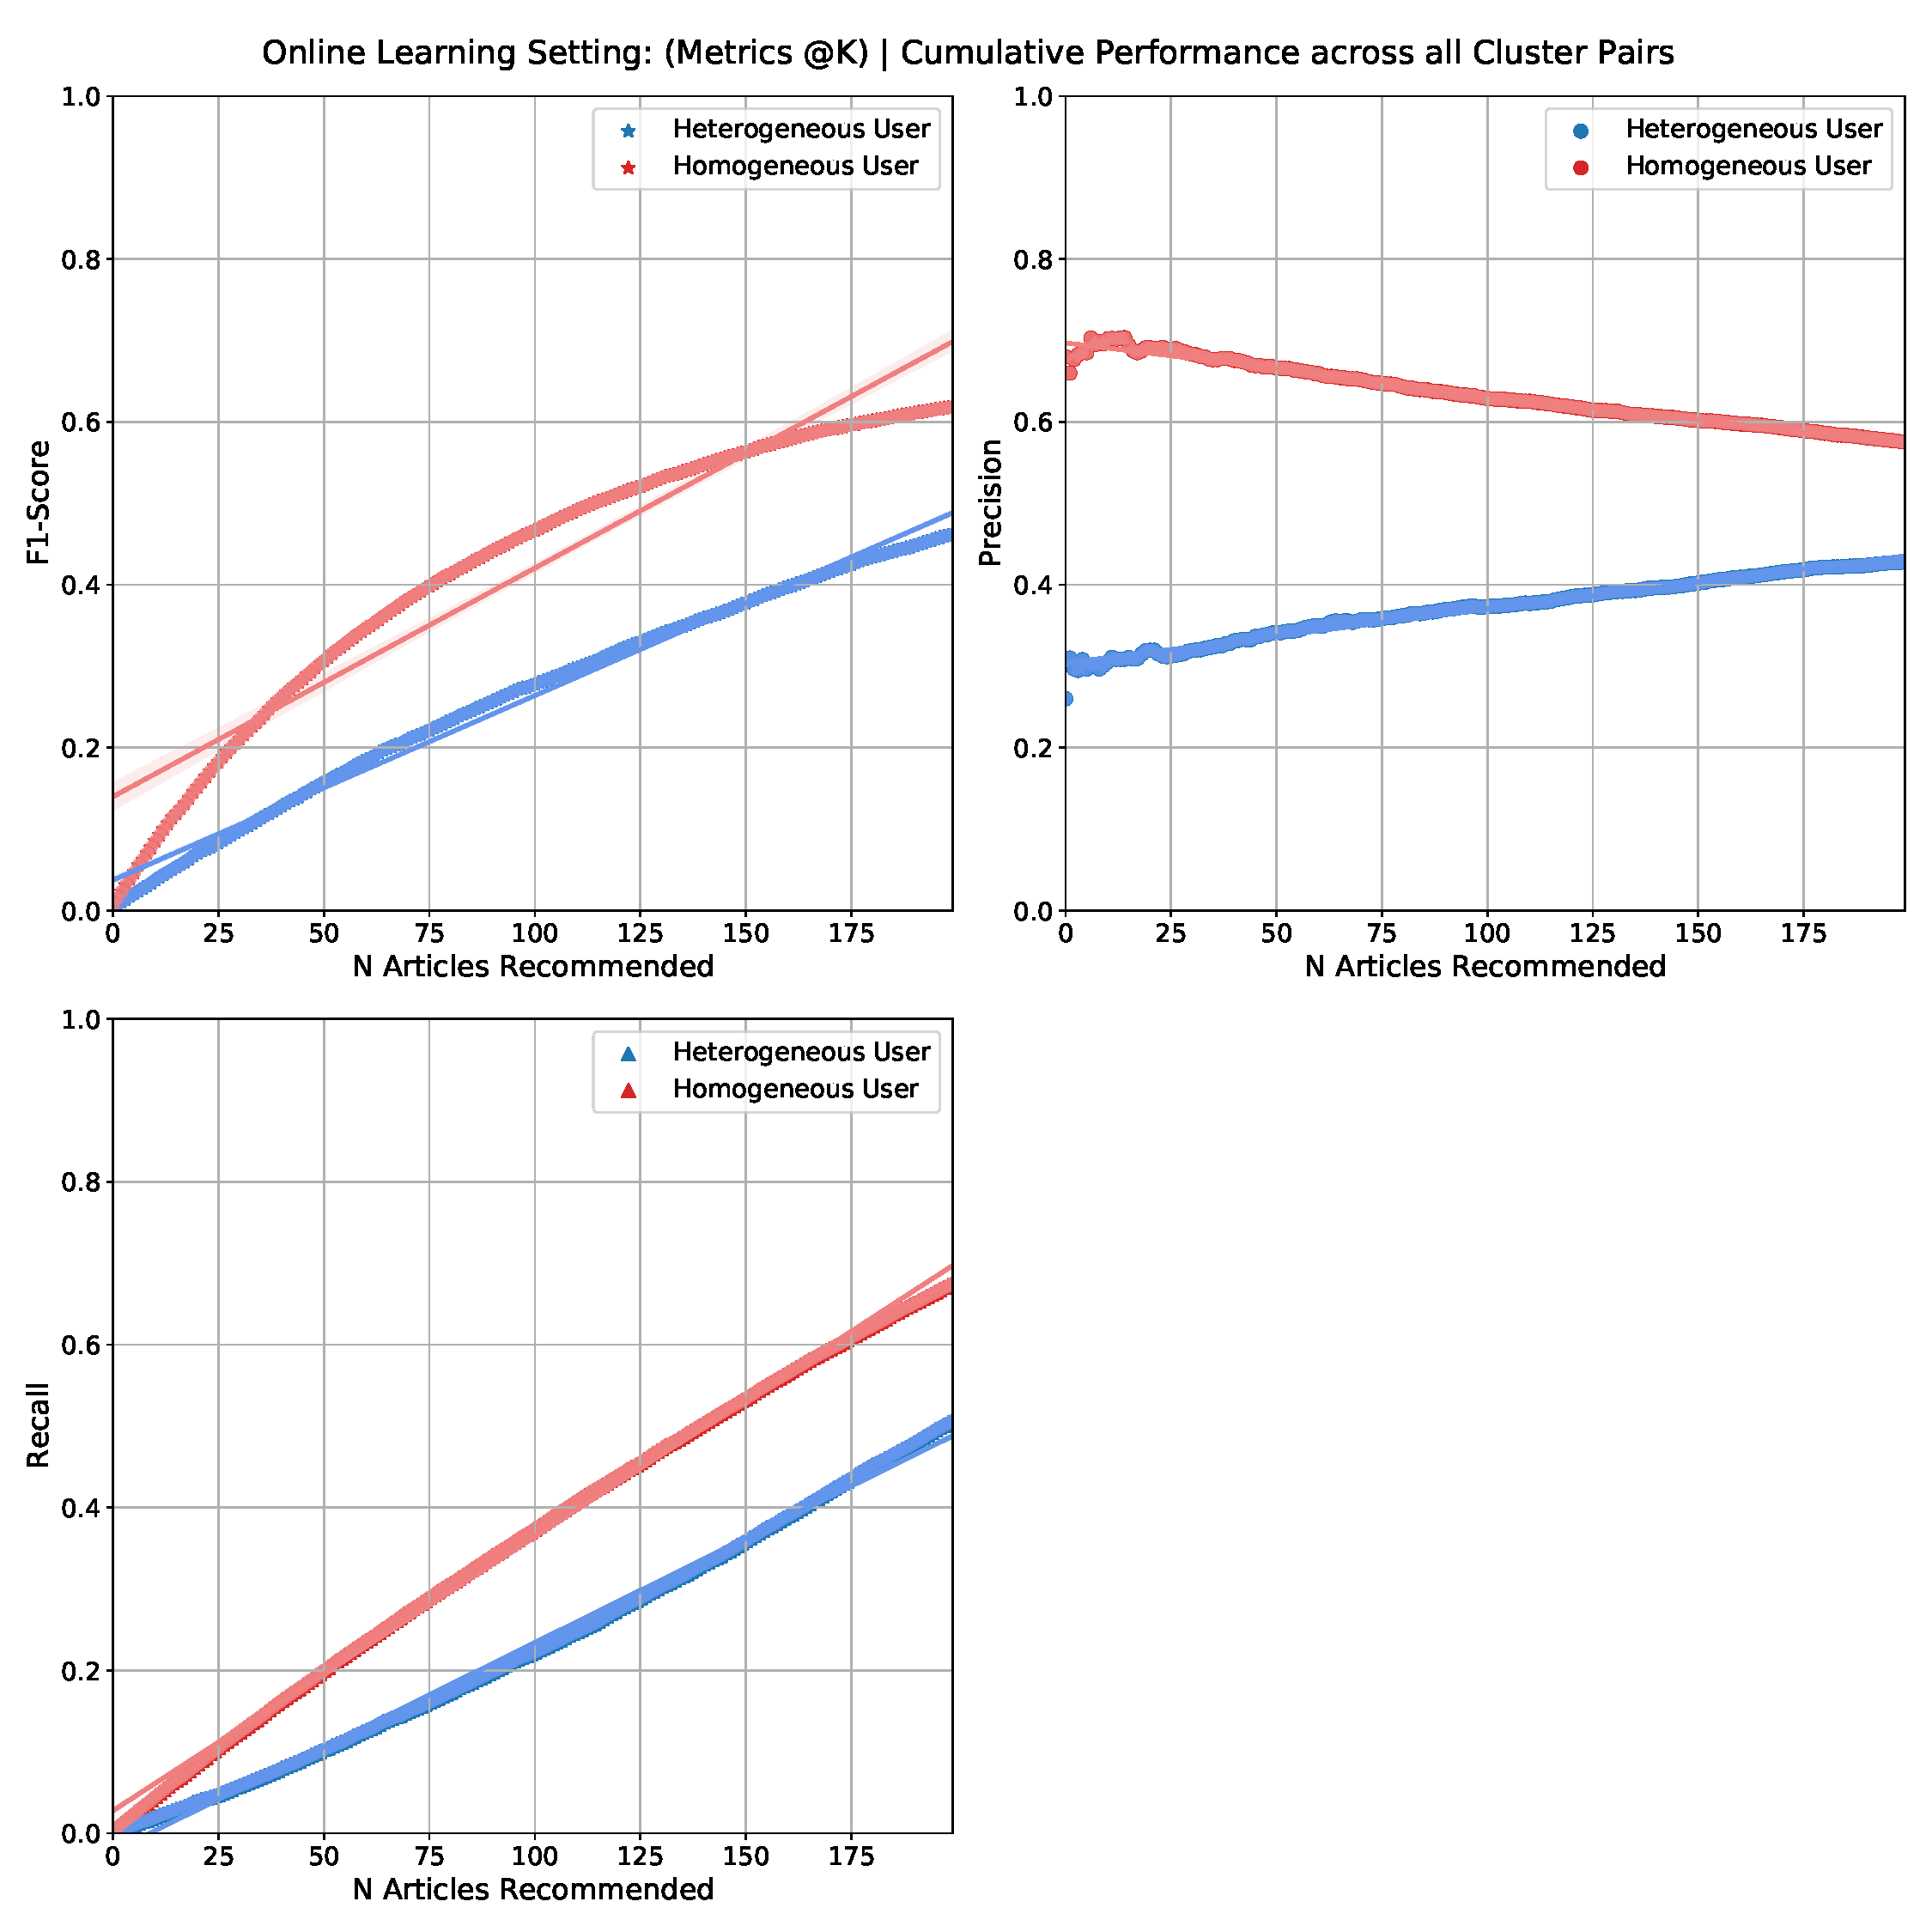
\includegraphics[width=0.8\textwidth]{Graphs/GLOVE/user_interaction_vs_model_performance_cumu.pdf}
\end{figure}
\vspace{-4ex}
\begin{figure}[H]
 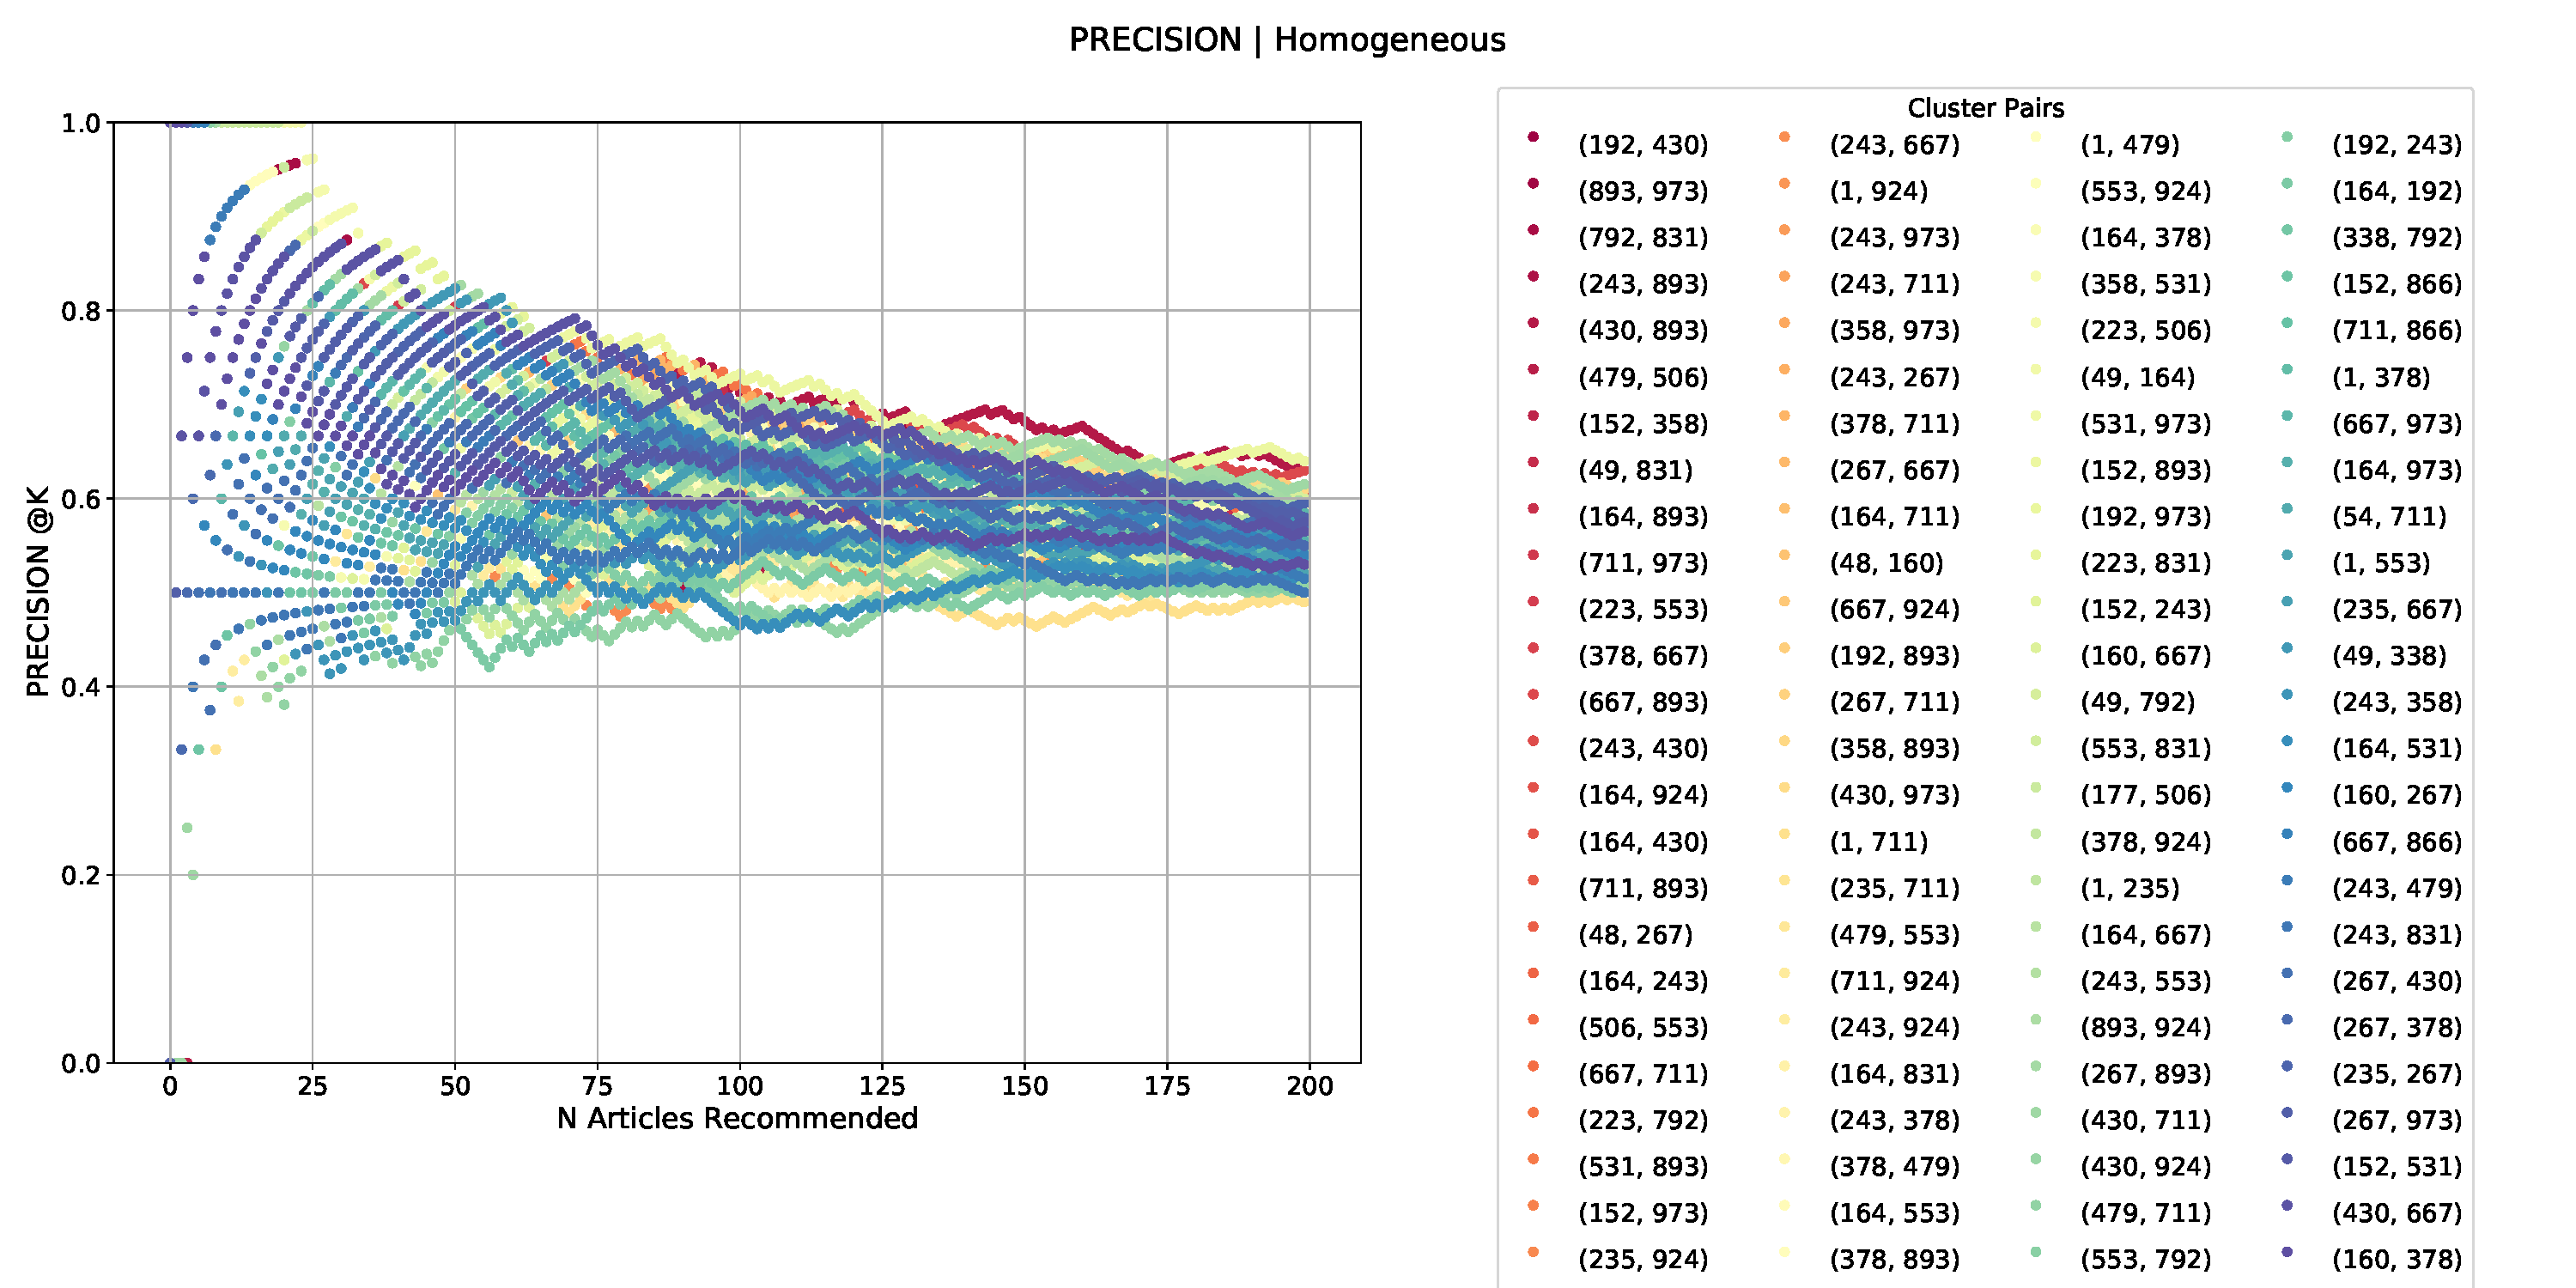
\includegraphics[width=1.0\textwidth]{Graphs/GLOVE/user_interaction_vs_model_performance_precision_all_cps_Homogeneous.pdf}
\end{figure}
\begin{figure}[H]
 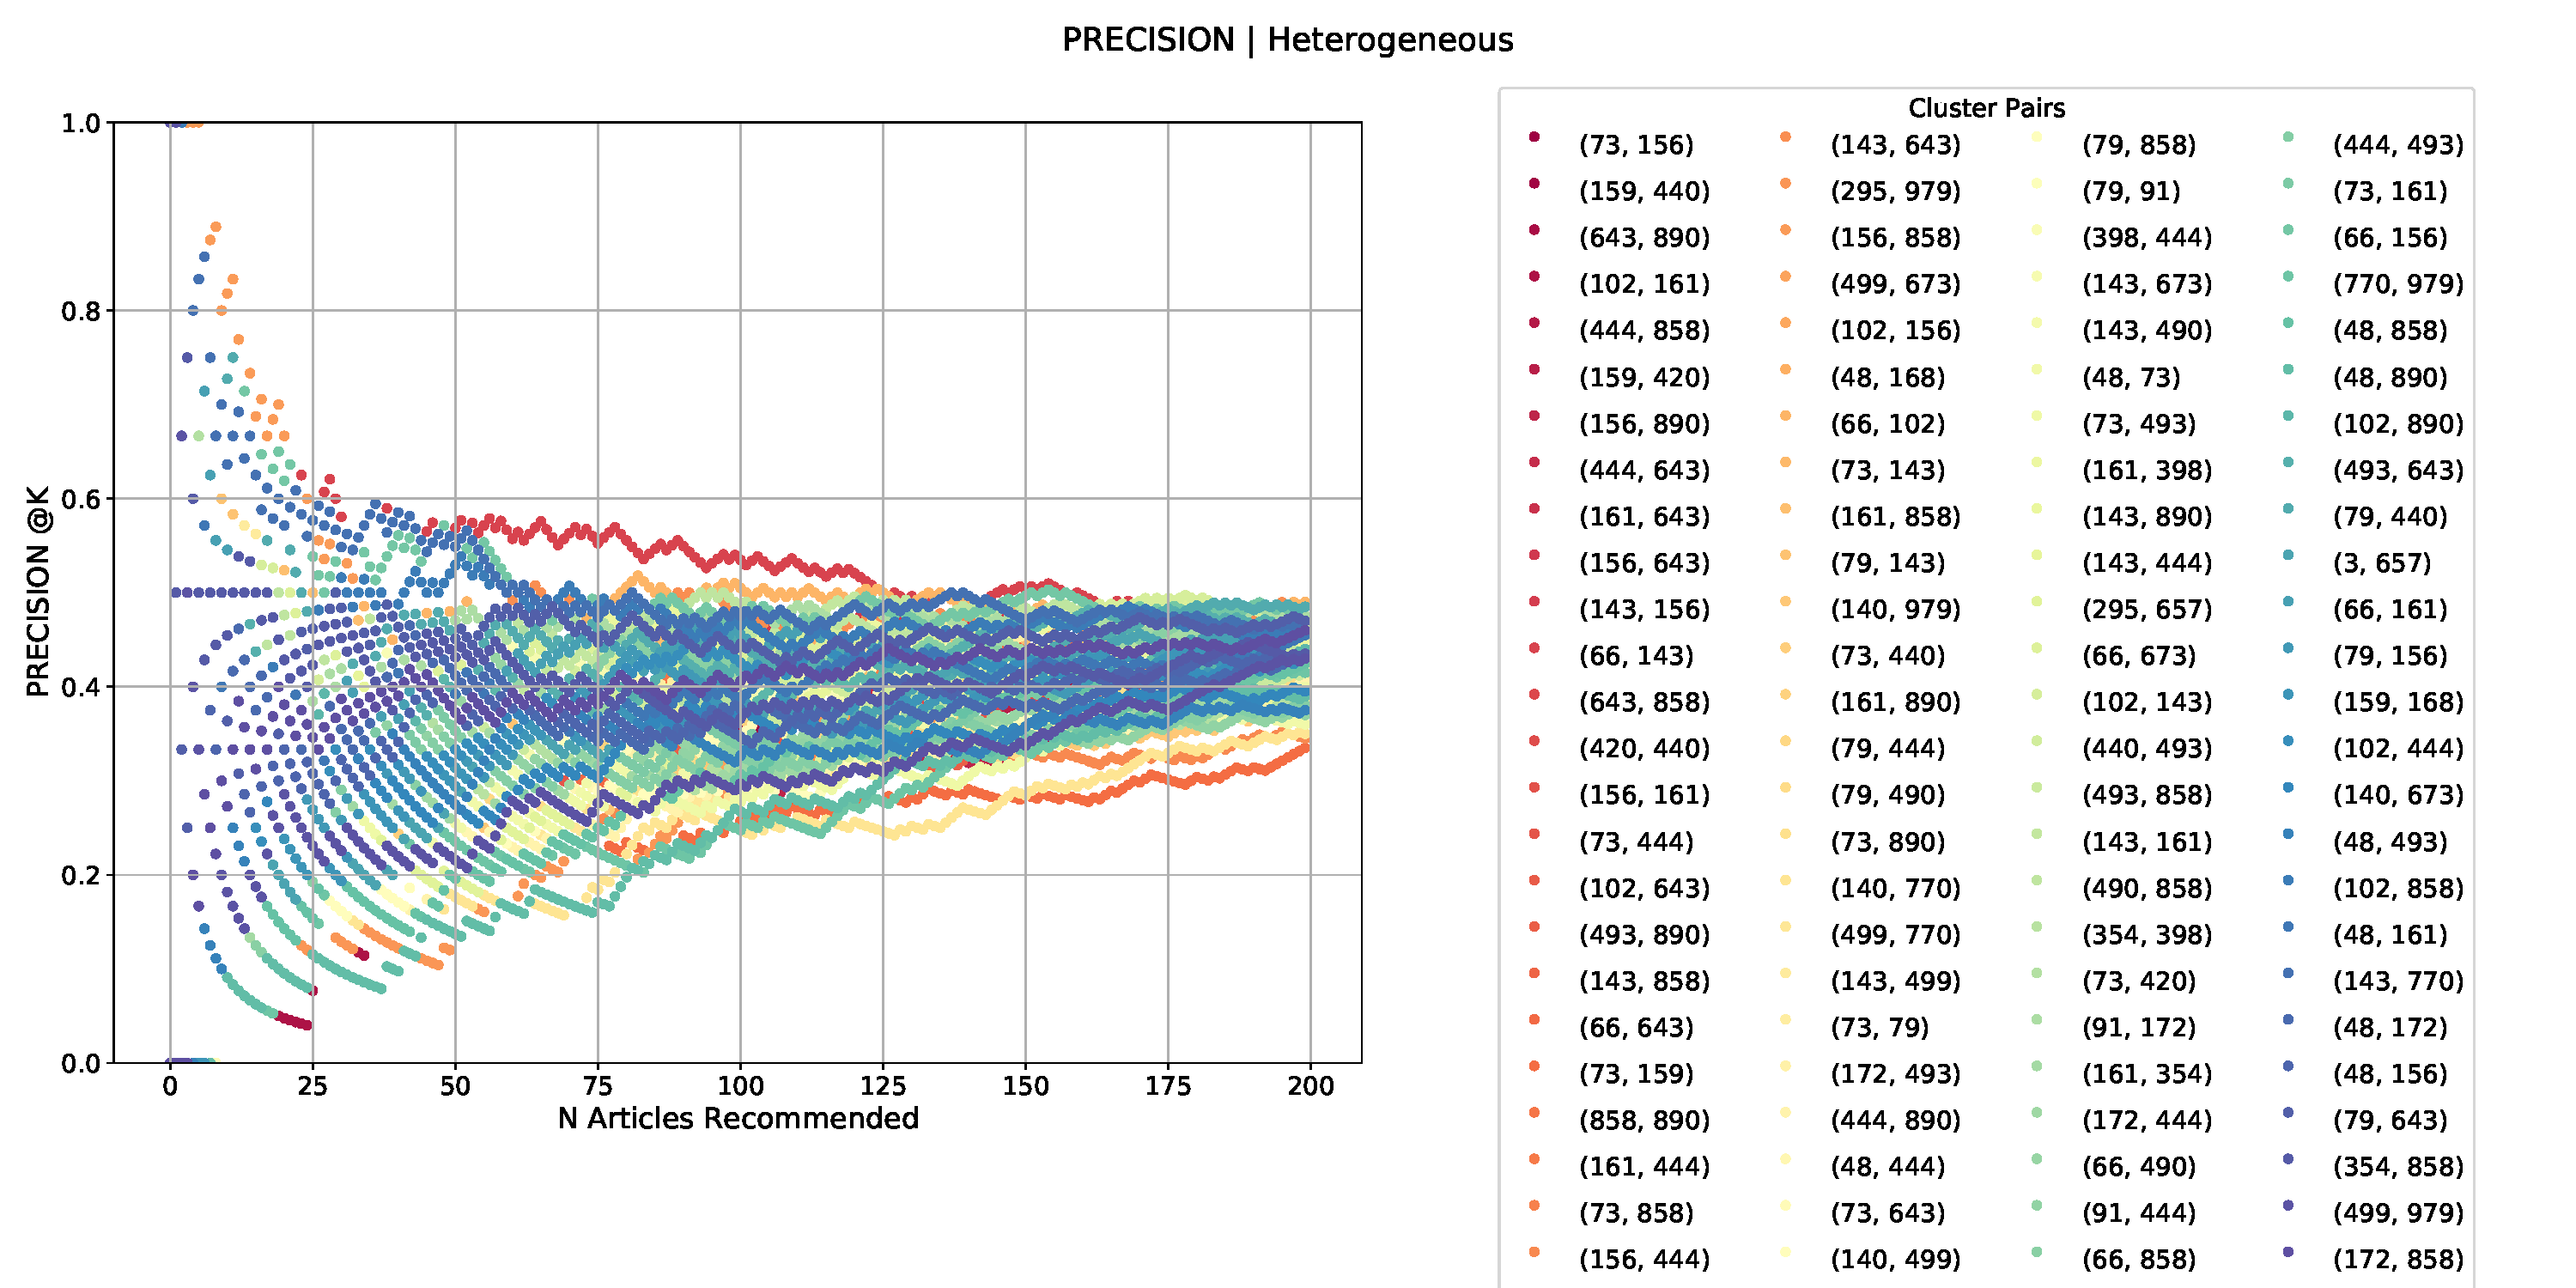
\includegraphics[width=1.0\textwidth]{Graphs/GLOVE/user_interaction_vs_model_performance_precision_all_cps_Heterogeneous.pdf}
\end{figure}
\begin{flushleft}
\begin{itemize}
    \item For Homogeneous Users here we see that their is a larger decrease in Precision compared to using TFIDF representations.
    \item For the Heterogeneous User we see a larger increase in Precision compared to using TFIDF representations
\end{itemize}
\end{flushleft}
\subsection{BERT}
\vspace{1ex}
\begin{figure}[H]
 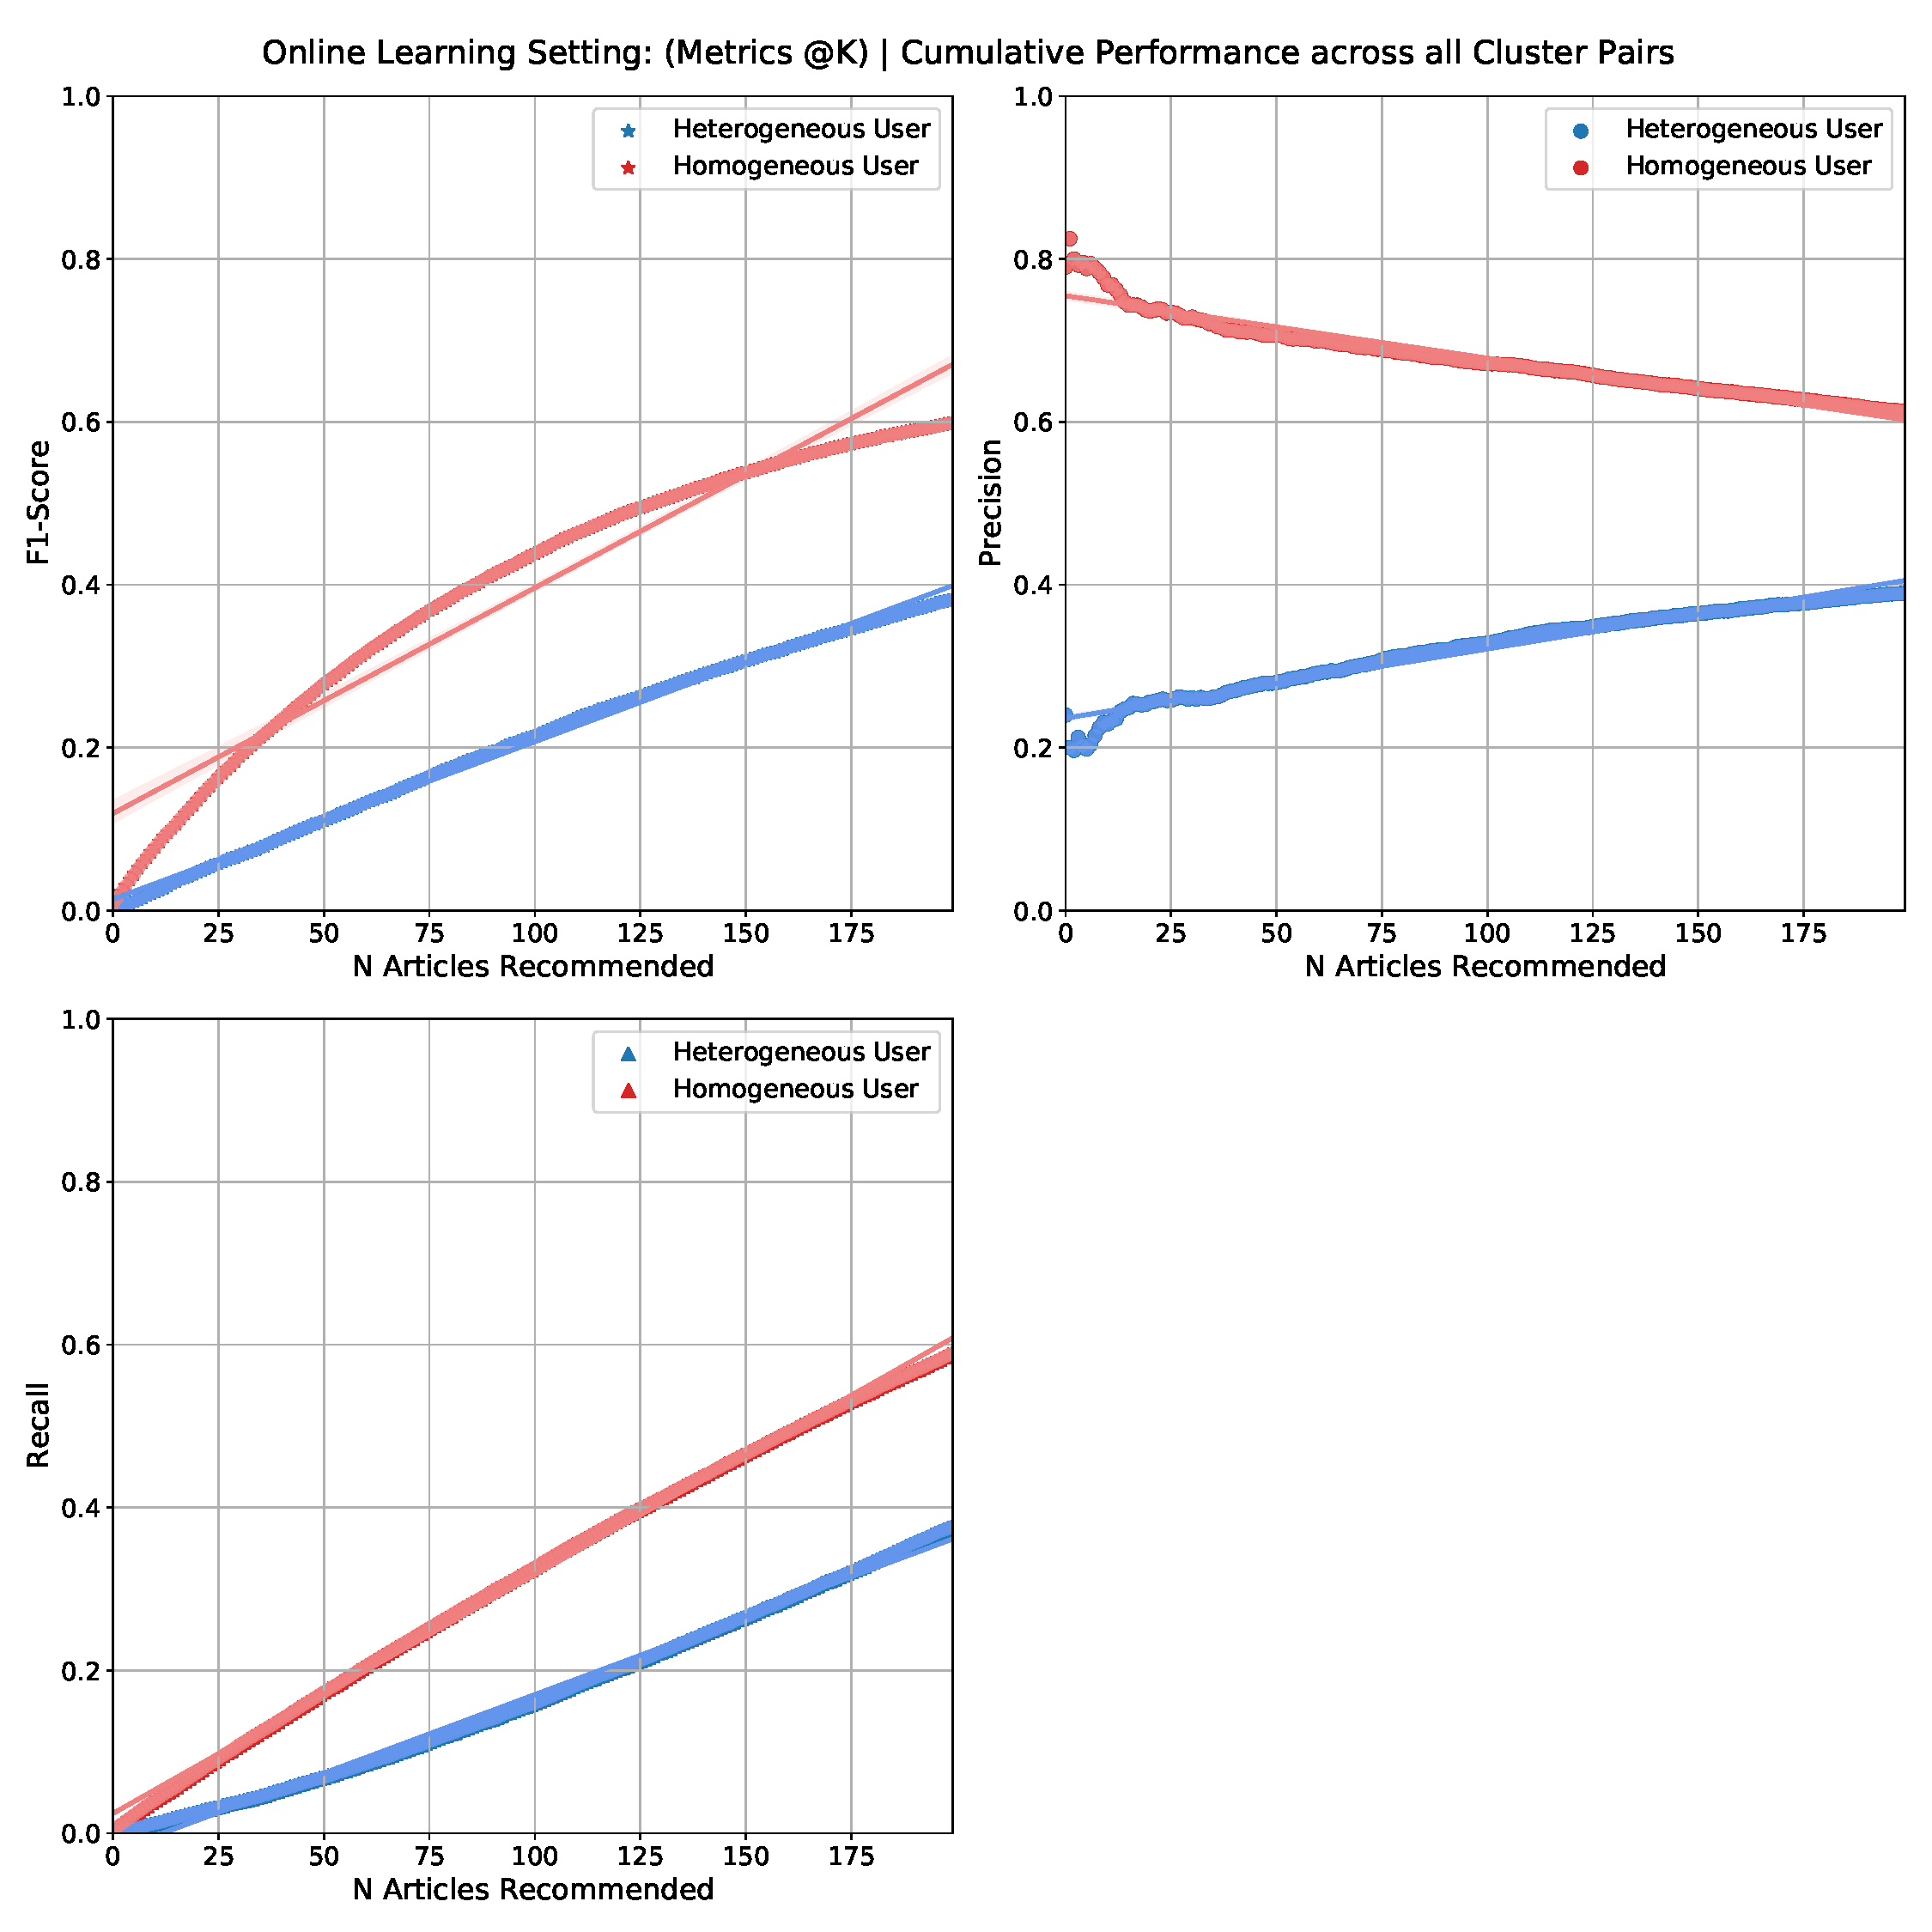
\includegraphics[width=0.8\textwidth]{Graphs/BERT/user_interaction_vs_model_performance_cumu.pdf}
\end{figure}
\vspace{-4ex}
\begin{figure}[H]
 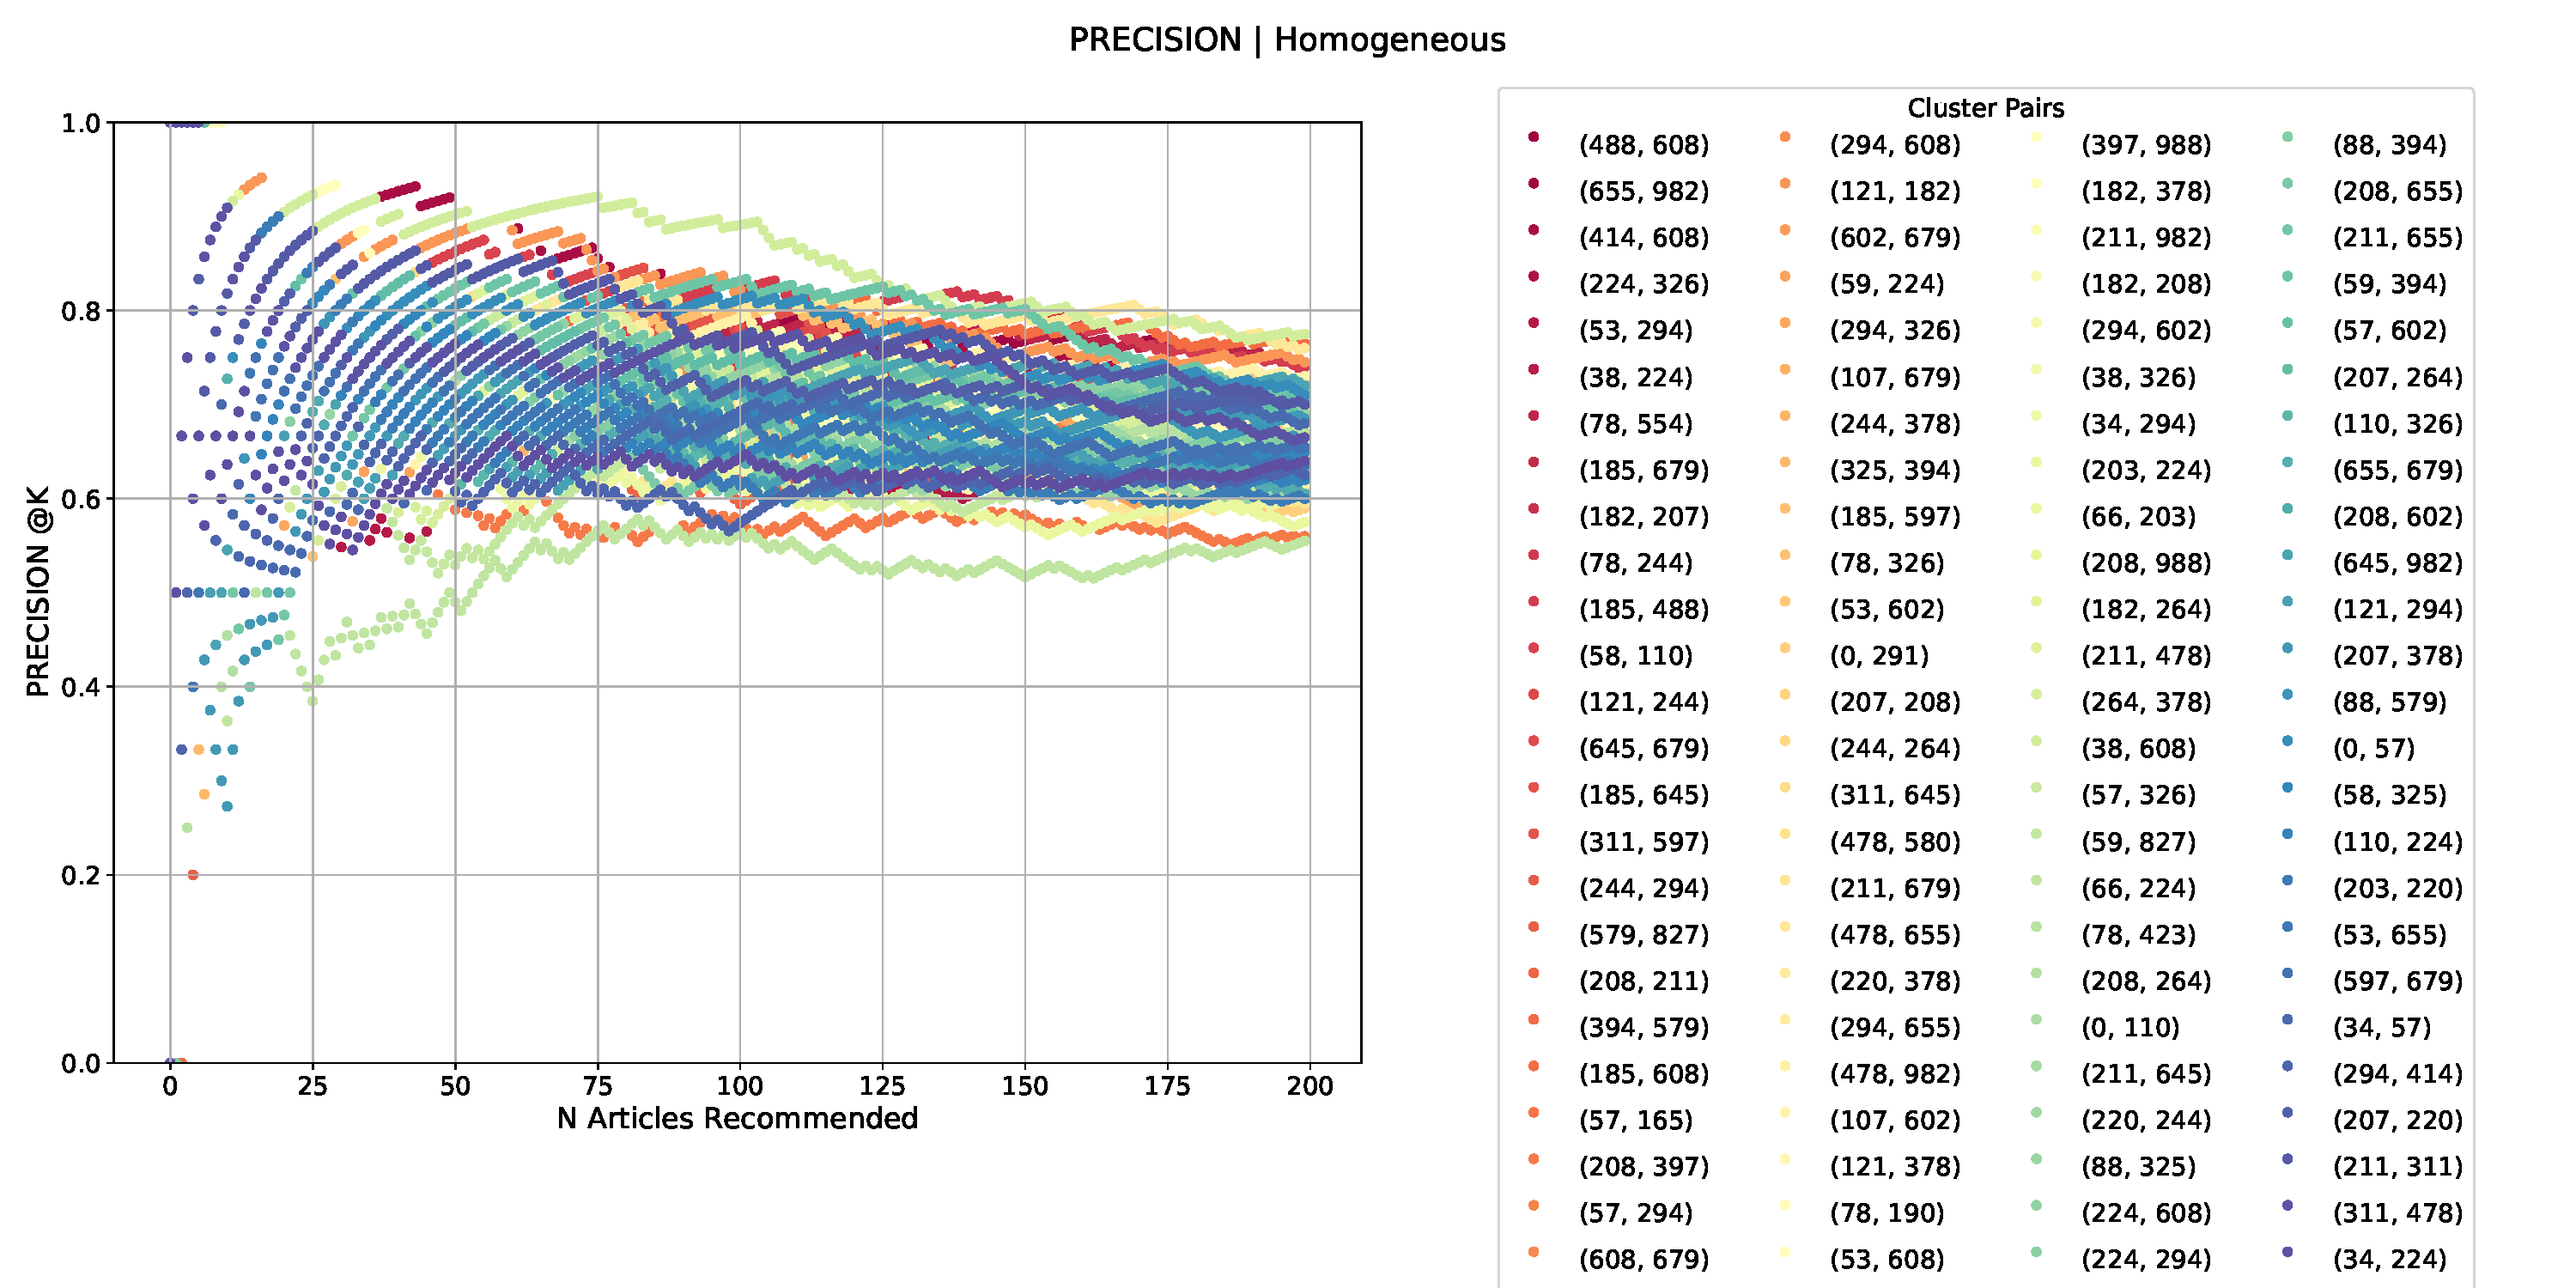
\includegraphics[width=1.0\textwidth]{Graphs/BERT/user_interaction_vs_model_performance_precision_all_cps_Homogeneous.pdf}
\end{figure}
\begin{figure}[H]
 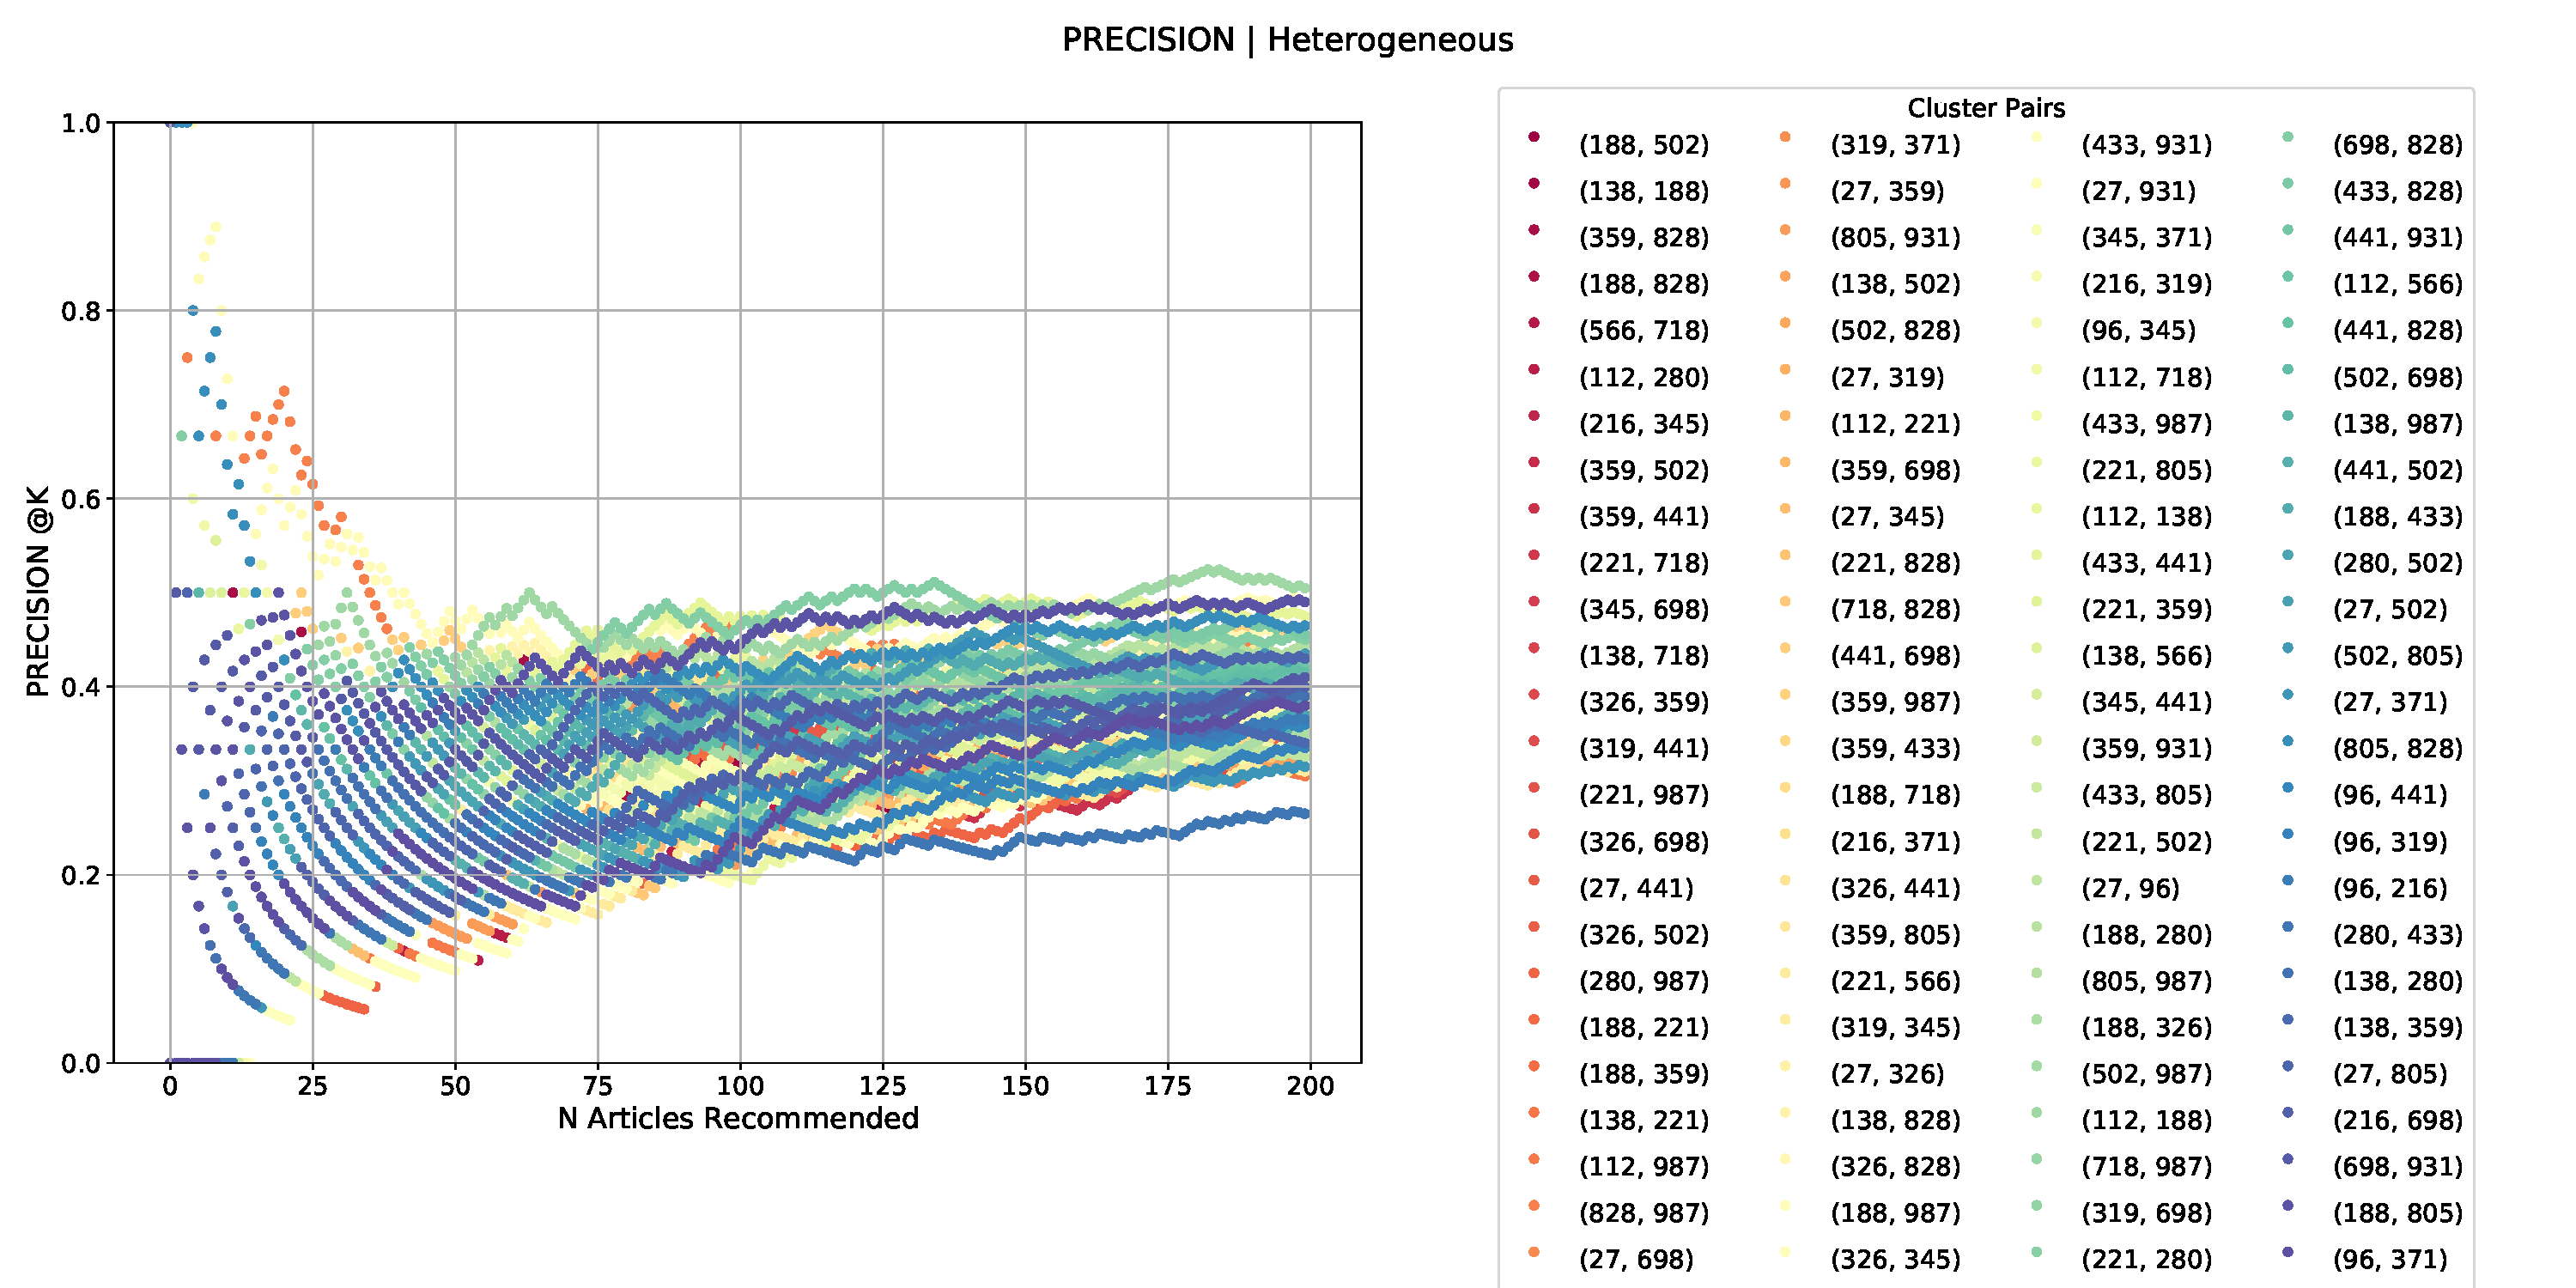
\includegraphics[width=1.0\textwidth]{Graphs/BERT/user_interaction_vs_model_performance_precision_all_cps_Heterogeneous.pdf}
\end{figure}
\begin{flushleft}
\begin{itemize}
    \item For Homogeneous Users here we see that their is a smaller decrease in Precision compared to using GLOVE representations.
    \item For the Heterogeneous User we see a smaller increase in Precision compared to using GLOVE representations
\end{itemize}
\end{flushleft}
\vspace{2ex}
\subsection{SUMMARY}
\begin{itemize}
    \item Using static or non-contextual embeddings helps the system's performance for Heterogeneous Users (according to Precision@K)
    \item Using dynamic or contextual embeddings helps the system's performance for Homogeneous Users.
\end{itemize}

\vspace{-1ex}
\newpage
\section{Baseline 3: How easy is it for the Recommendation System to detect a change in topics}
\begin{flushleft}
We want to know how the recommendation system performs in detecting a change in topics , so we measure the performance of the system using a single cluster and compare it against our online setting performance (shown in the above baseline). 
\end{flushleft}
\subsection{TF-IDF}
\begin{flushleft}
\begin{itemize}
    \item Similar trend in Precision@K occurs here (compared to baseline 2 - Homogeneous User). 
    \item  When we compare these scores to graphs in Baseline 2 we definitely see that the recommendation system tends to have an easier time when only one topic is concerned compared to 2 different topics, so the model is having a hard time in identifying a change in topic.
\end{itemize}
\end{flushleft}
% \vspace{-5ex}
\begin{figure}[H]
 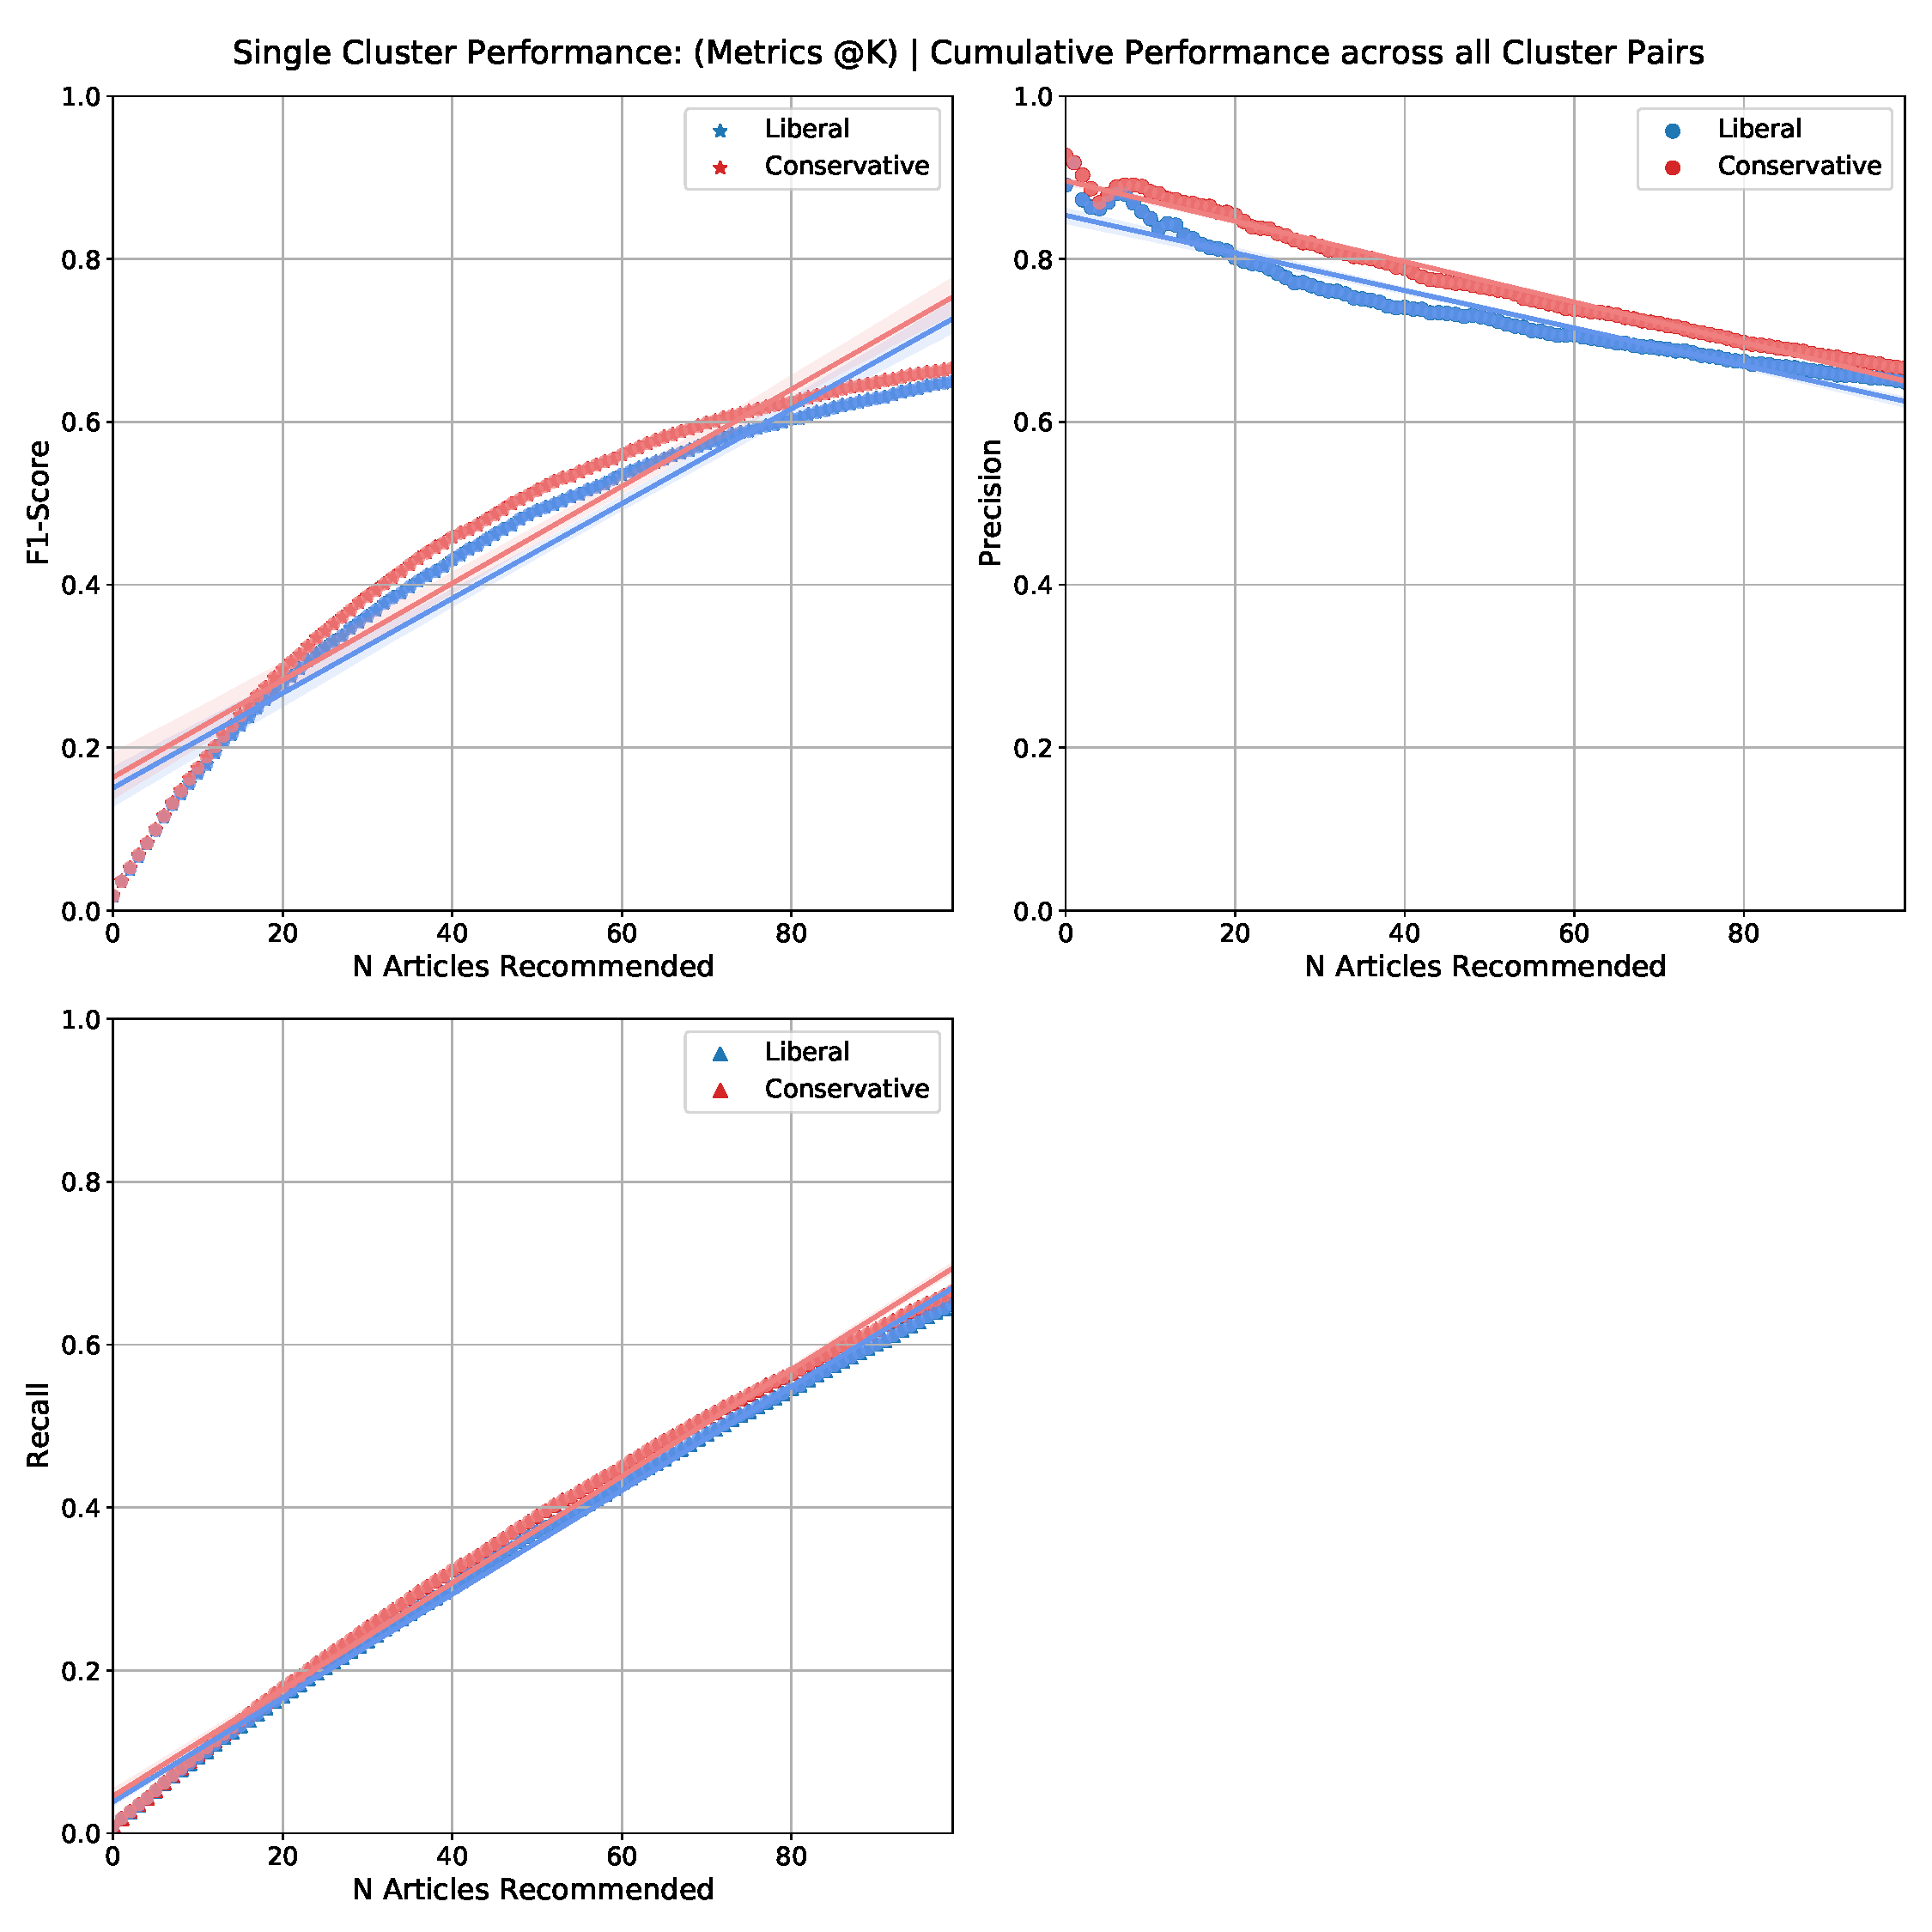
\includegraphics[width=0.8\textwidth]{Graphs/TFIDF/user_interaction_vs_model_performance_cumu_single_cluster.pdf}
\end{figure}
\begin{figure}[H]
 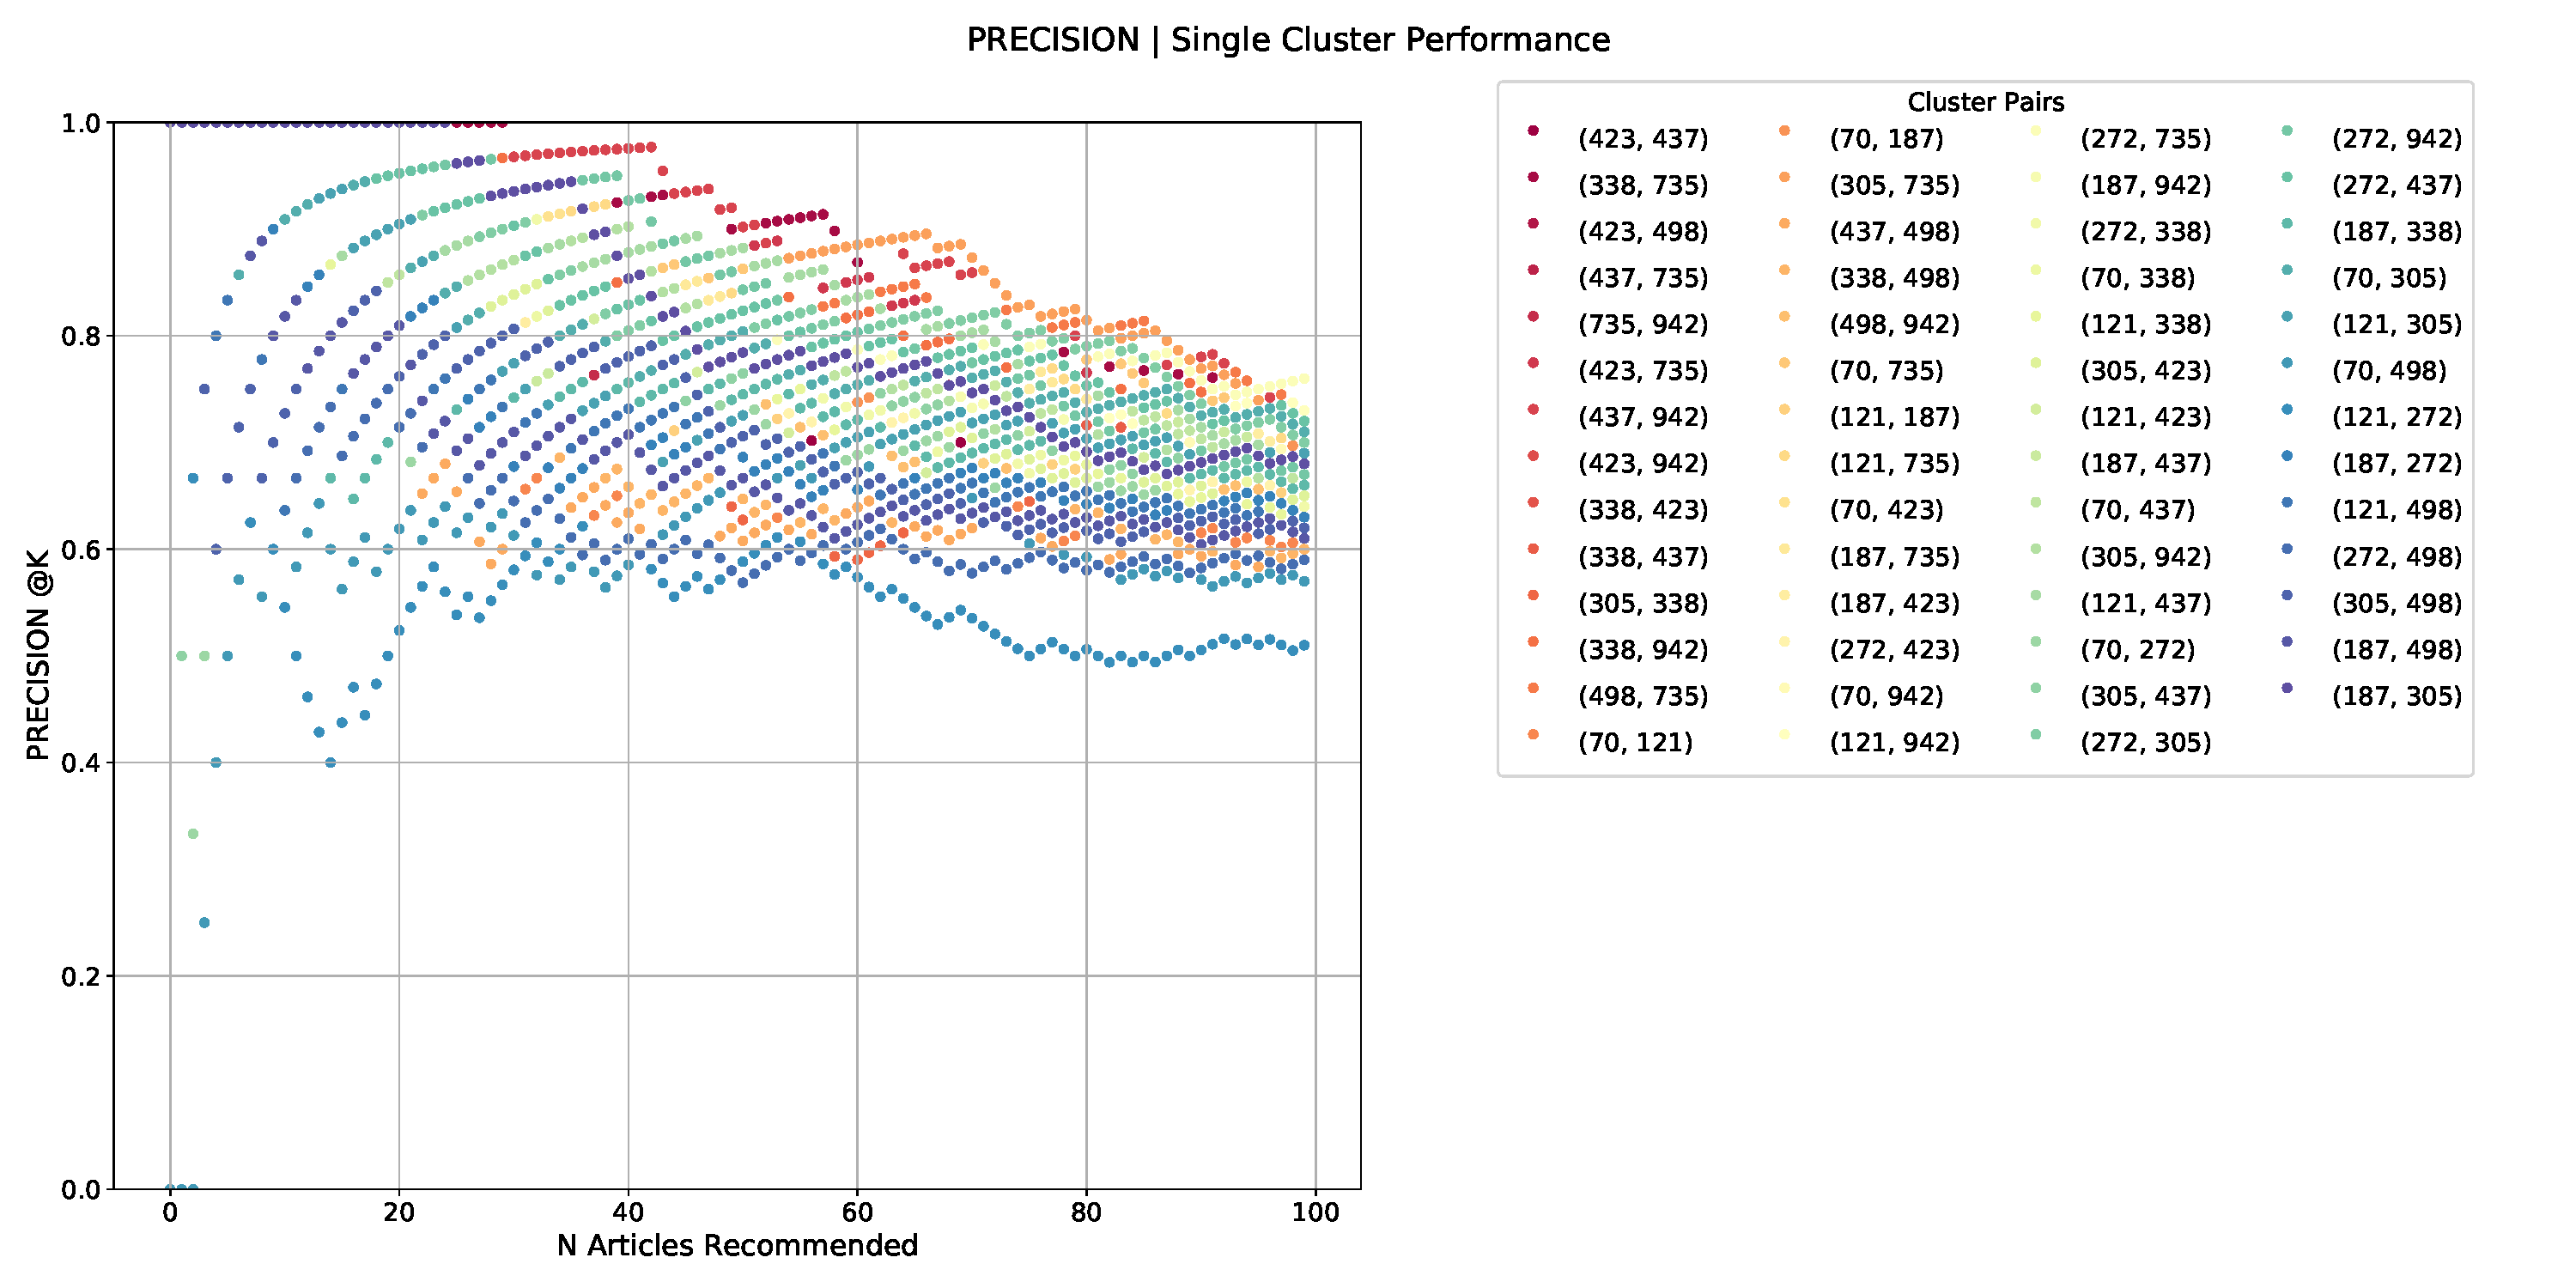
\includegraphics[width=1.0\textwidth]{Graphs/TFIDF/user_interaction_vs_model_performance_precision_all_cps_single_cluster.pdf}
\end{figure}
\subsection{Glove}
\begin{flushleft}
\begin{itemize}
    \item Similar trend in Precision@K occurs here (compared to baseline 2 - Homogeneous User). 
    \item  Lower Precision compared to TFIDF Representations
\end{itemize}
\end{flushleft}
% \vspace{-5ex}
\begin{figure}[H]
 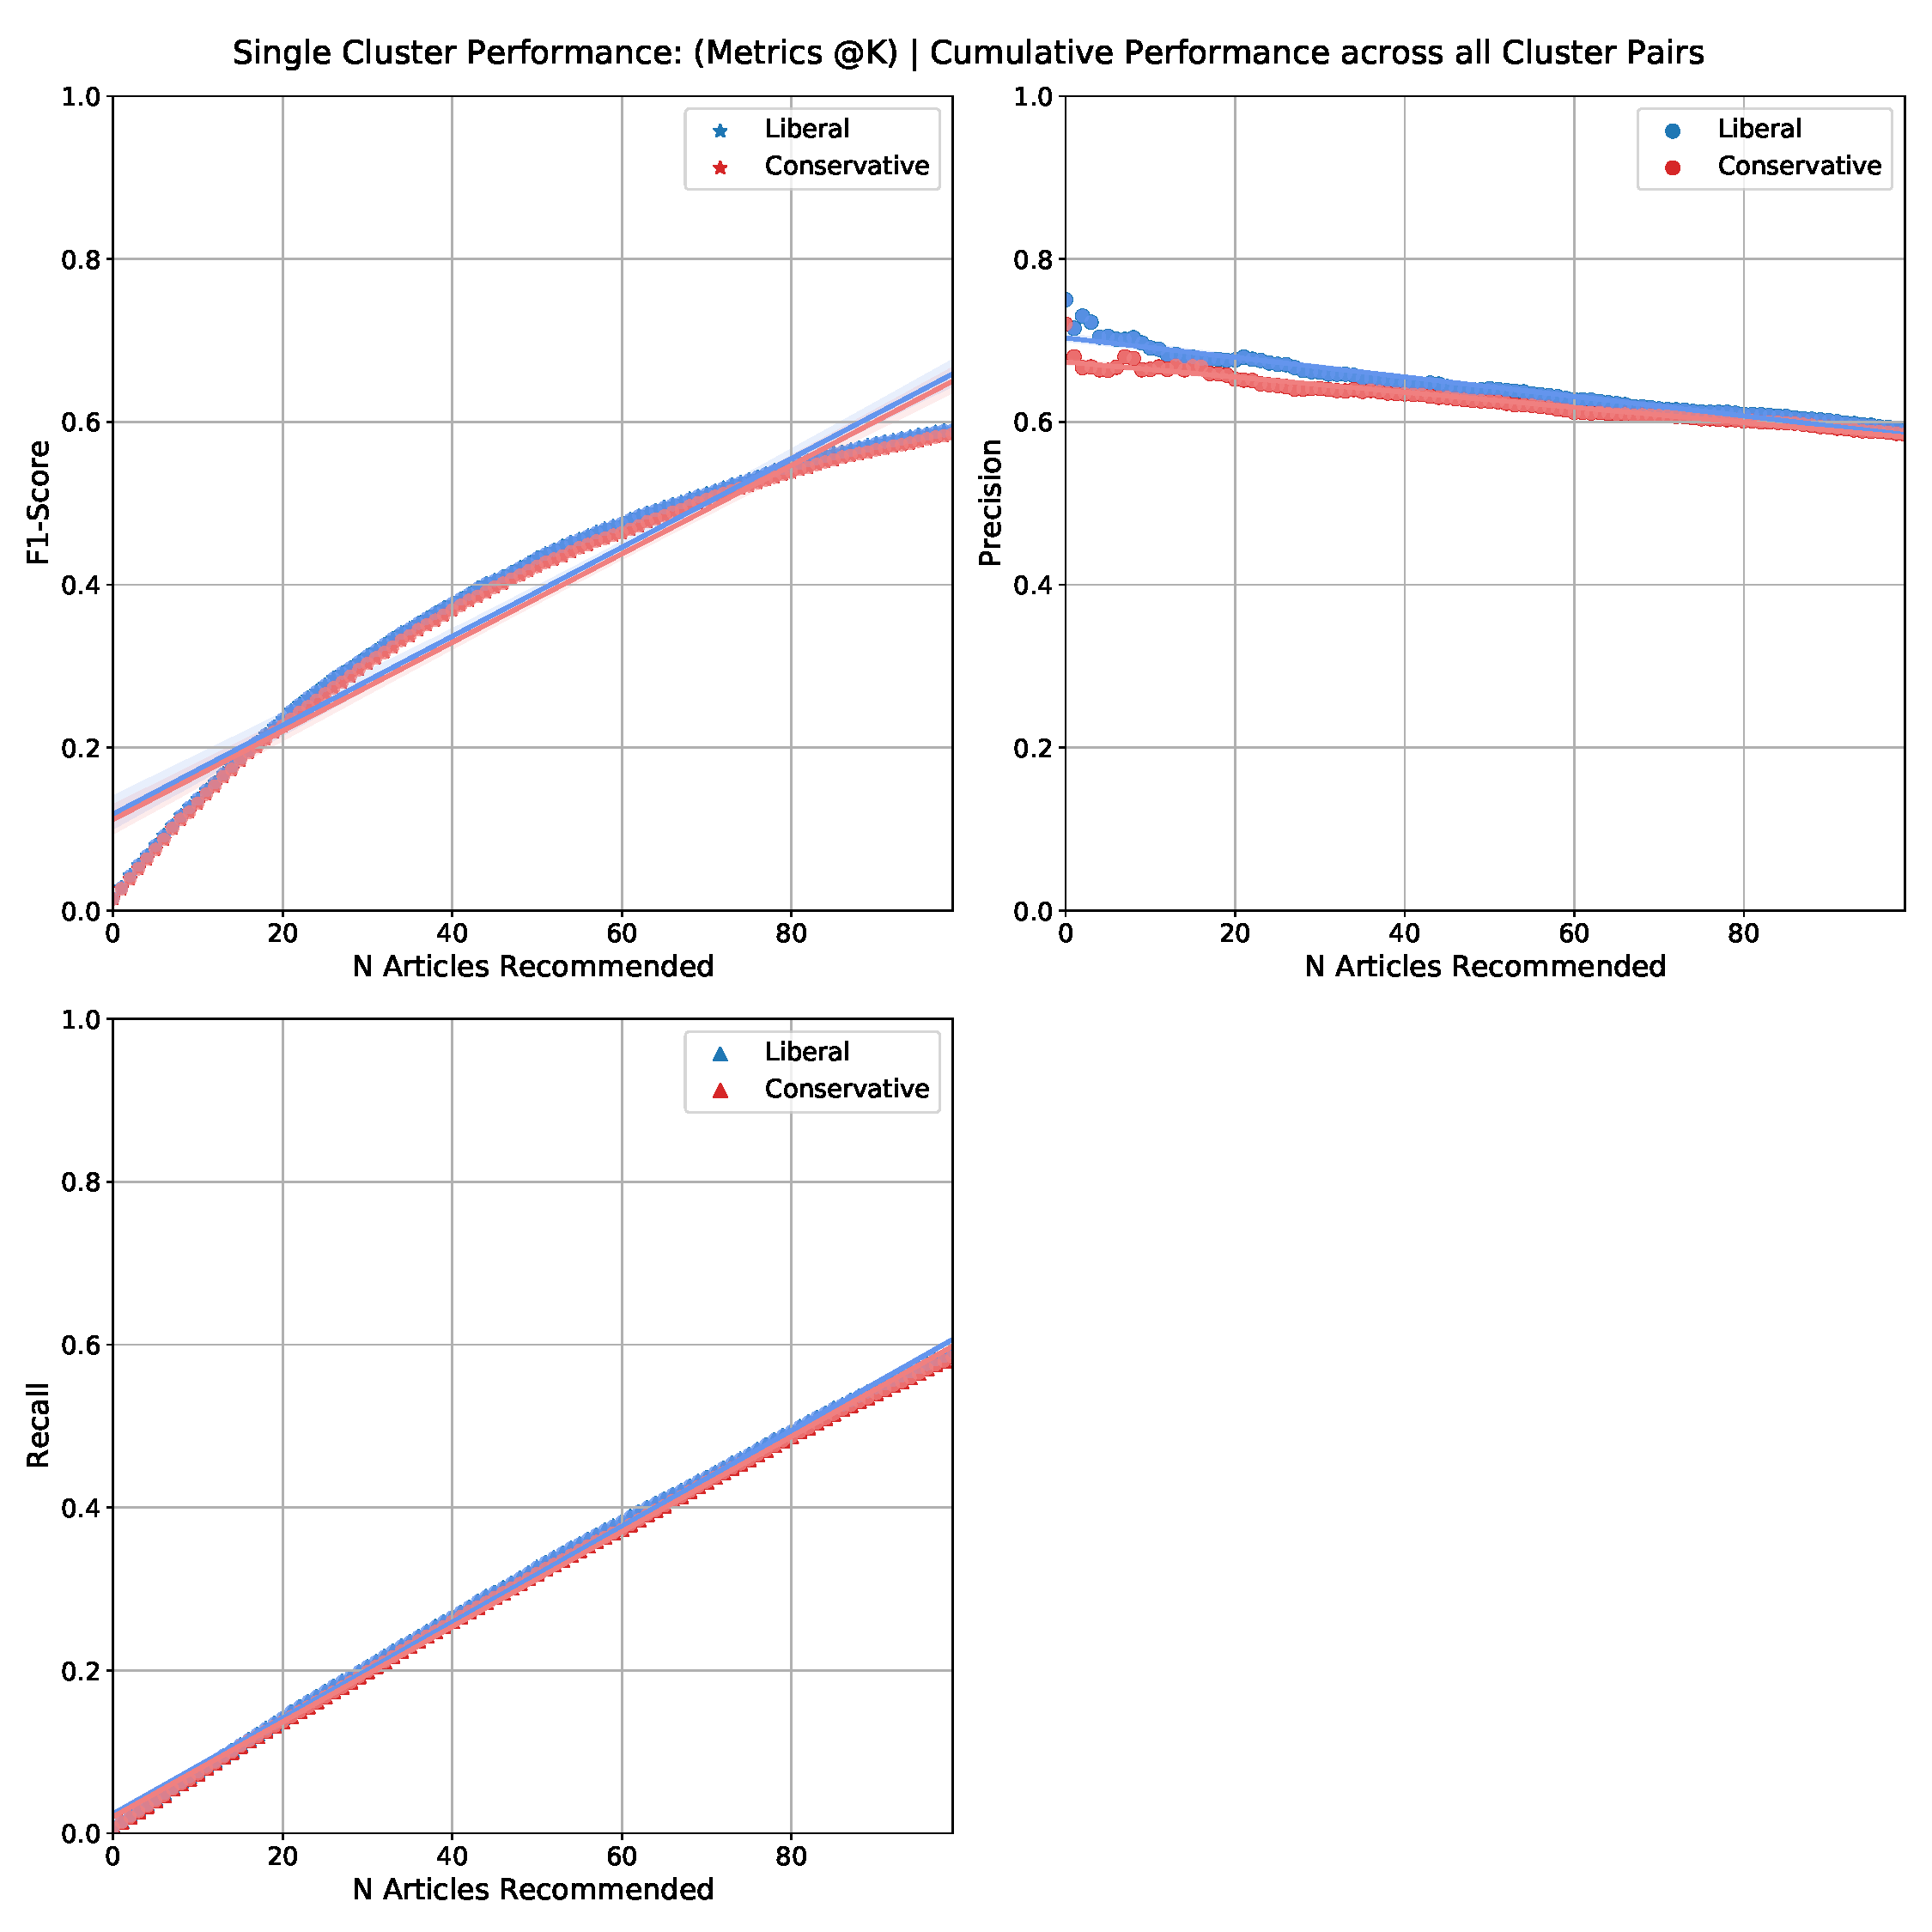
\includegraphics[width=0.8\textwidth]{Graphs/GLOVE/user_interaction_vs_model_performance_cumu_single_cluster.pdf}
\end{figure}
\begin{figure}[H]
 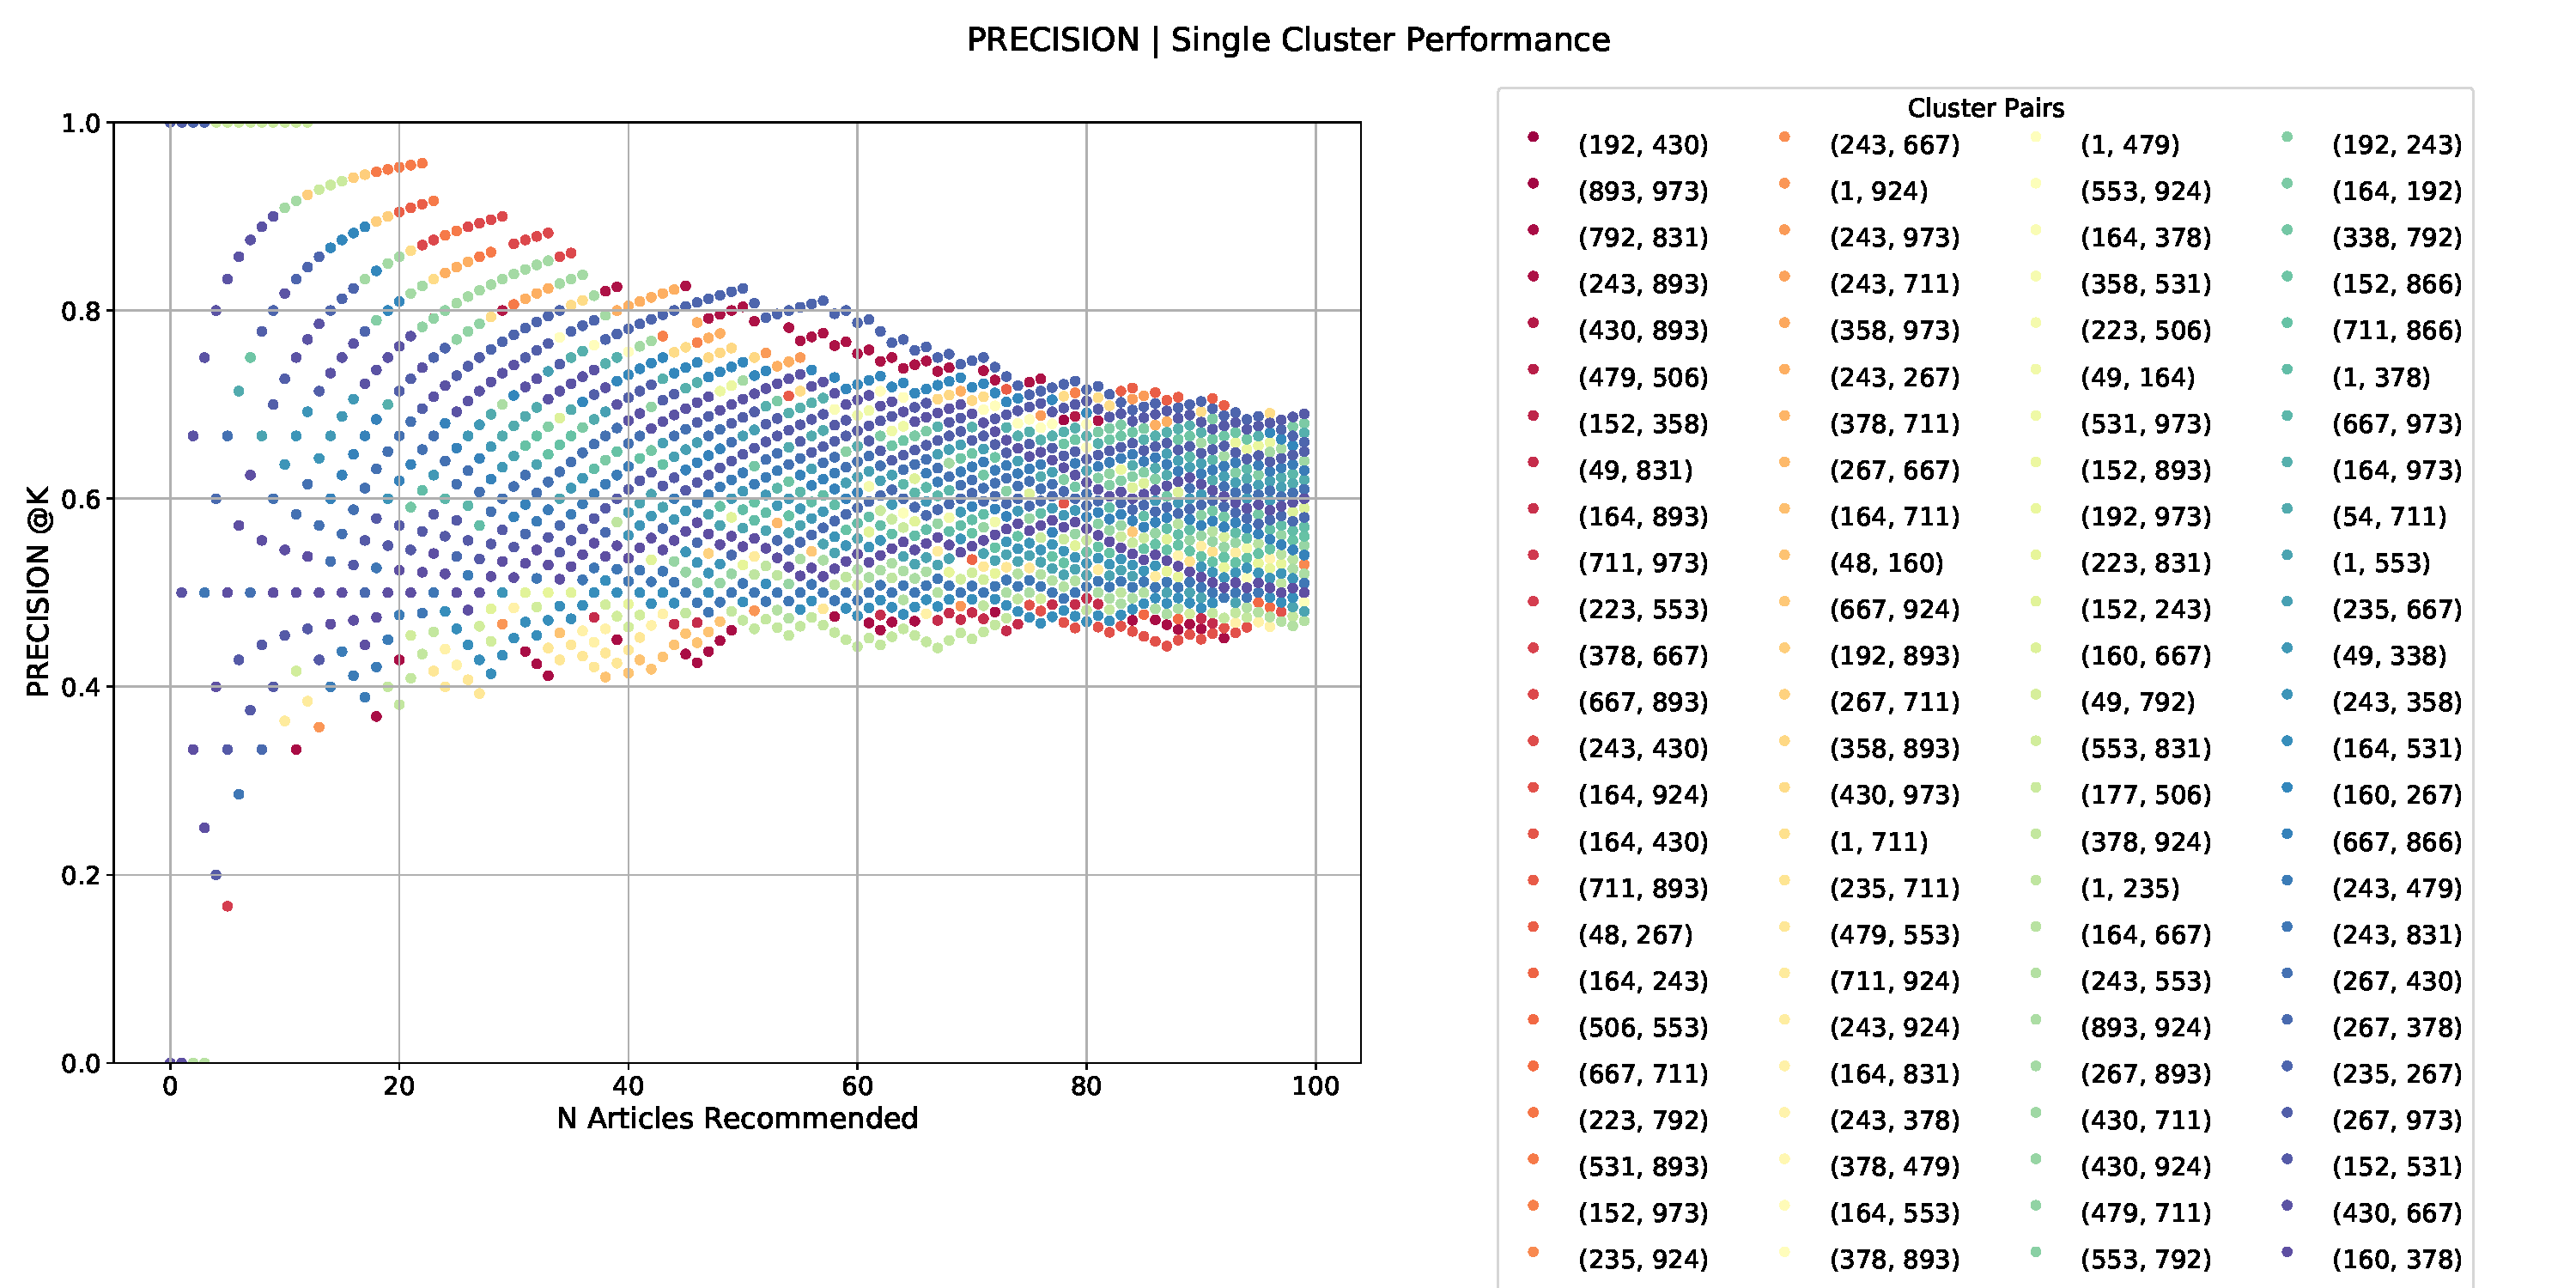
\includegraphics[width=1.0\textwidth]{Graphs/GLOVE/user_interaction_vs_model_performance_precision_all_cps_single_cluster.pdf}
\end{figure}
\subsection{BERT}
\begin{flushleft}
\begin{itemize}
    \item Similar trend in Precision@K occurs here (compared to baseline 2 - Homogeneous User). 
    \item  Lower Precision trend compared to TFIDF representations but better than Glove
\end{itemize}
\end{flushleft}
% \vspace{-5ex}
\begin{figure}[H]
 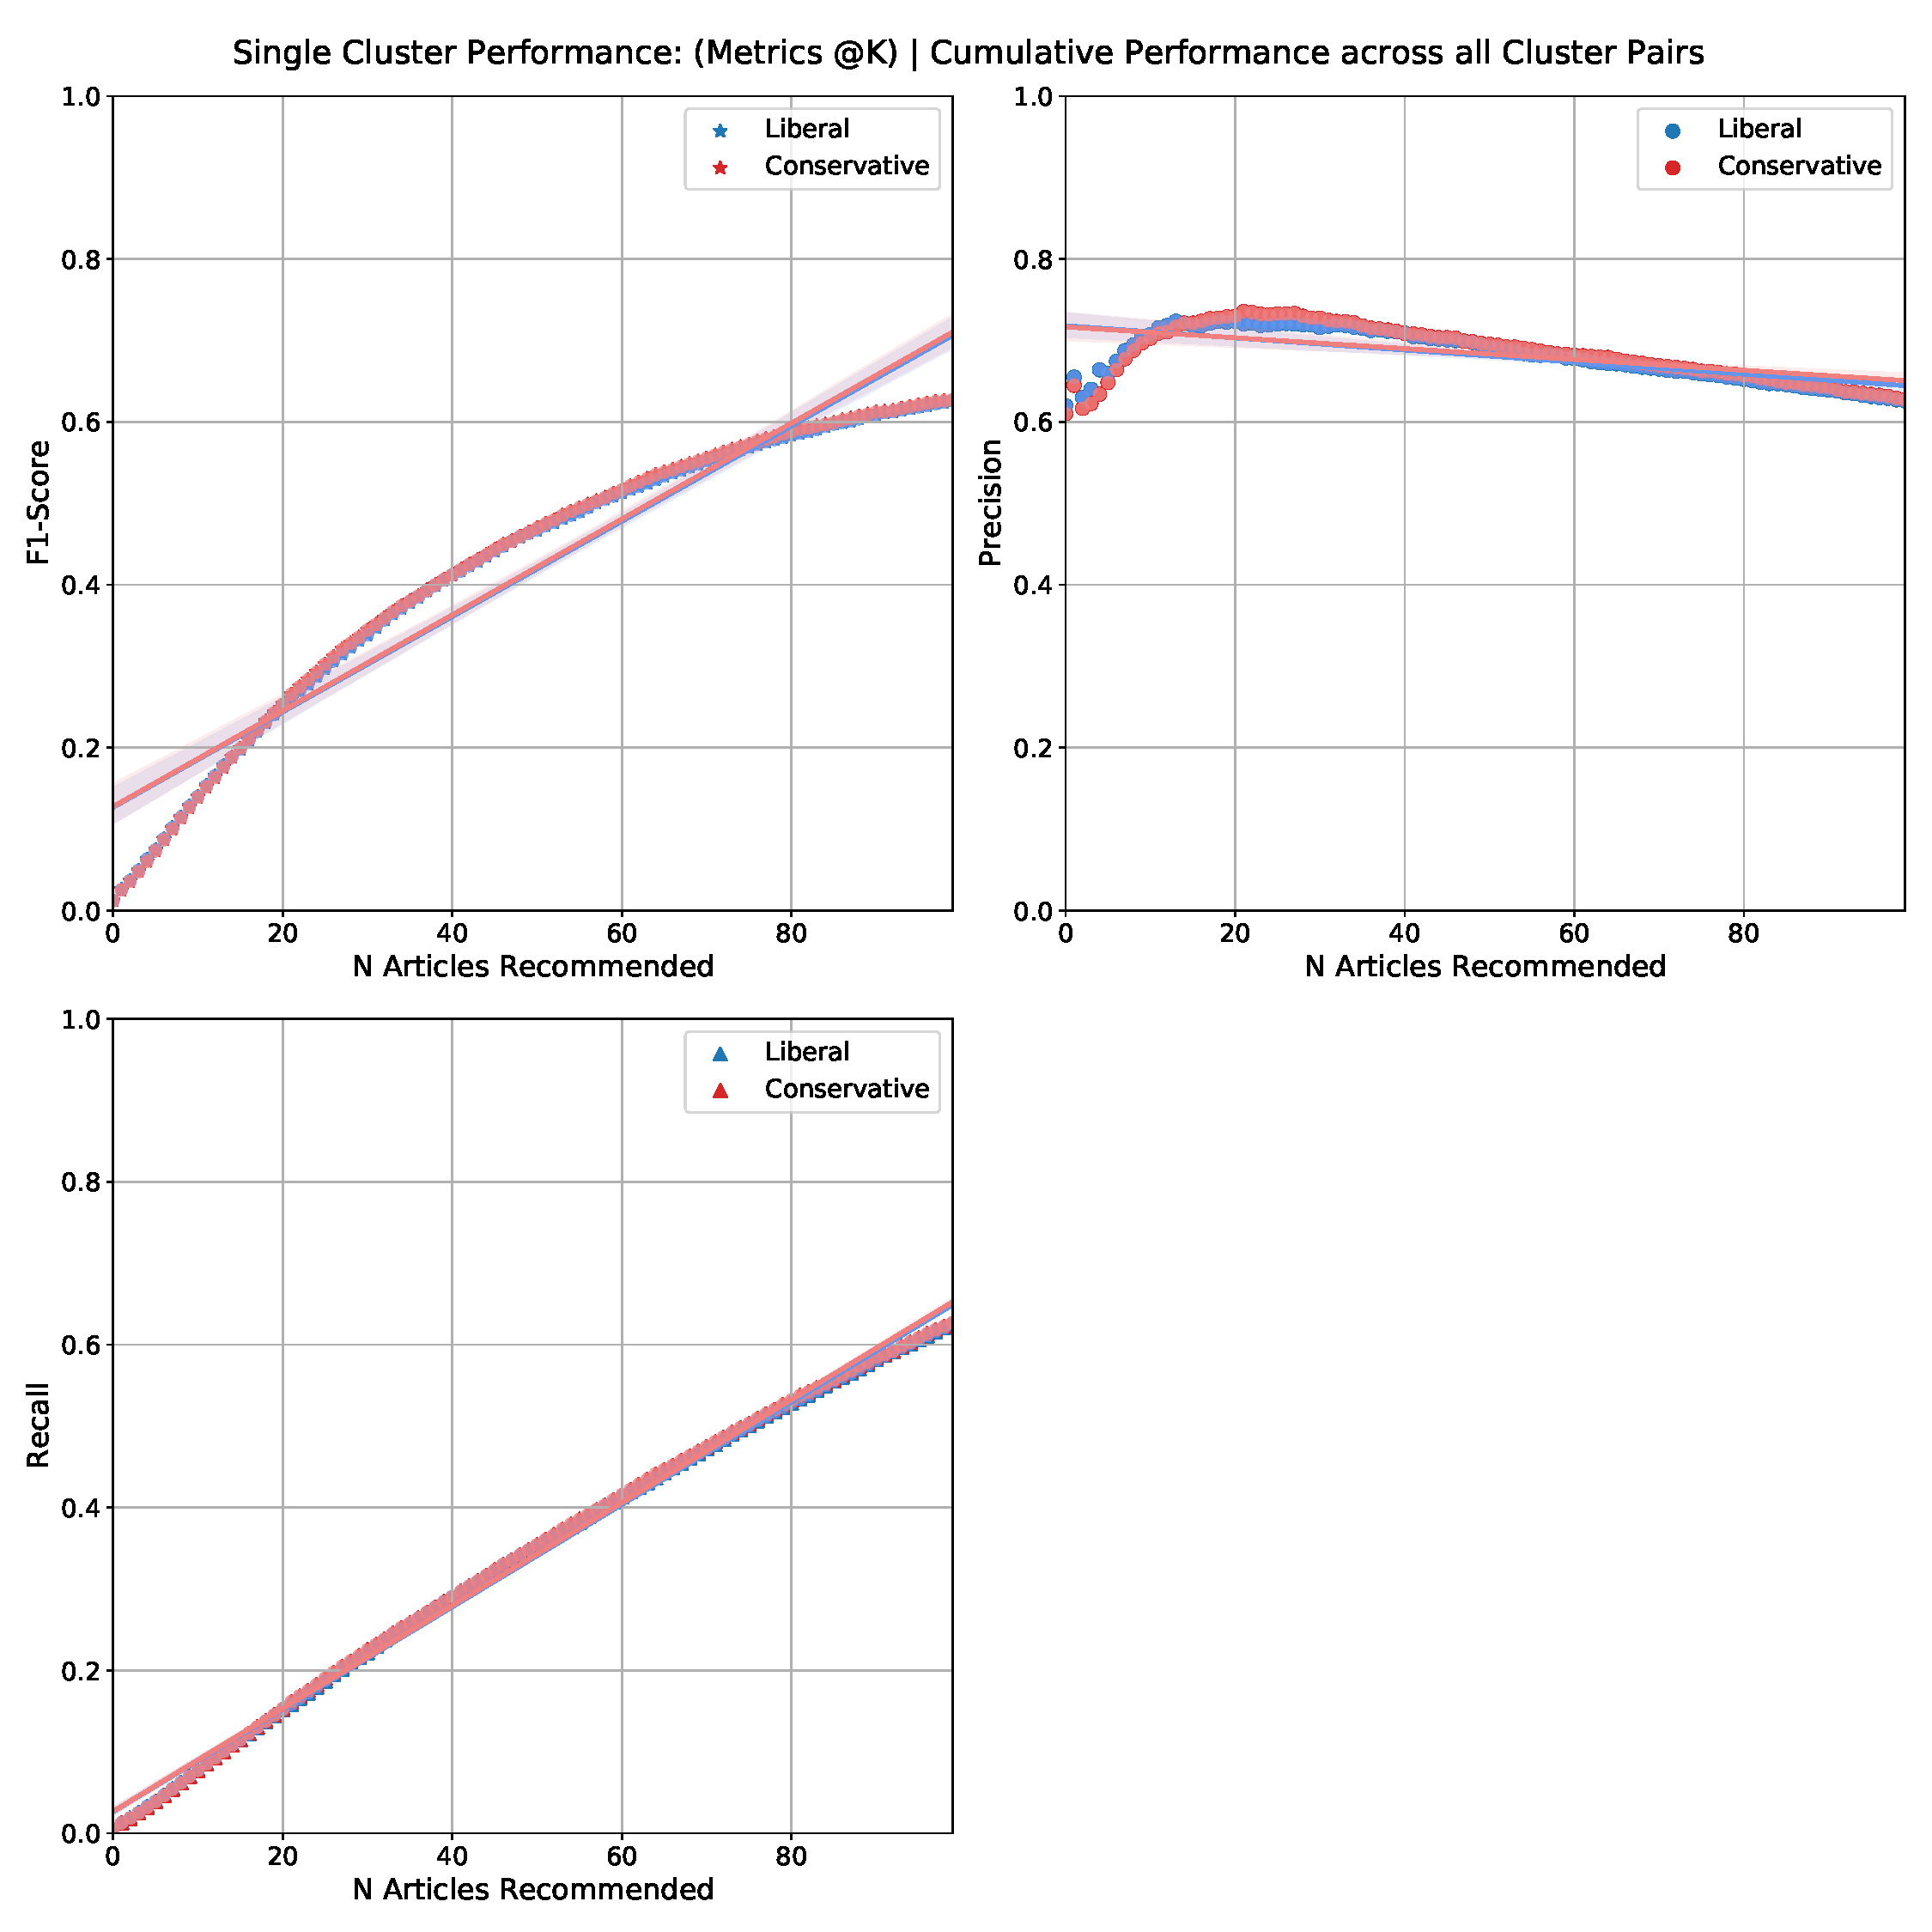
\includegraphics[width=0.8\textwidth]{Graphs/BERT/user_interaction_vs_model_performance_cumu_single_cluster.pdf}
\end{figure}
\begin{figure}[H]
 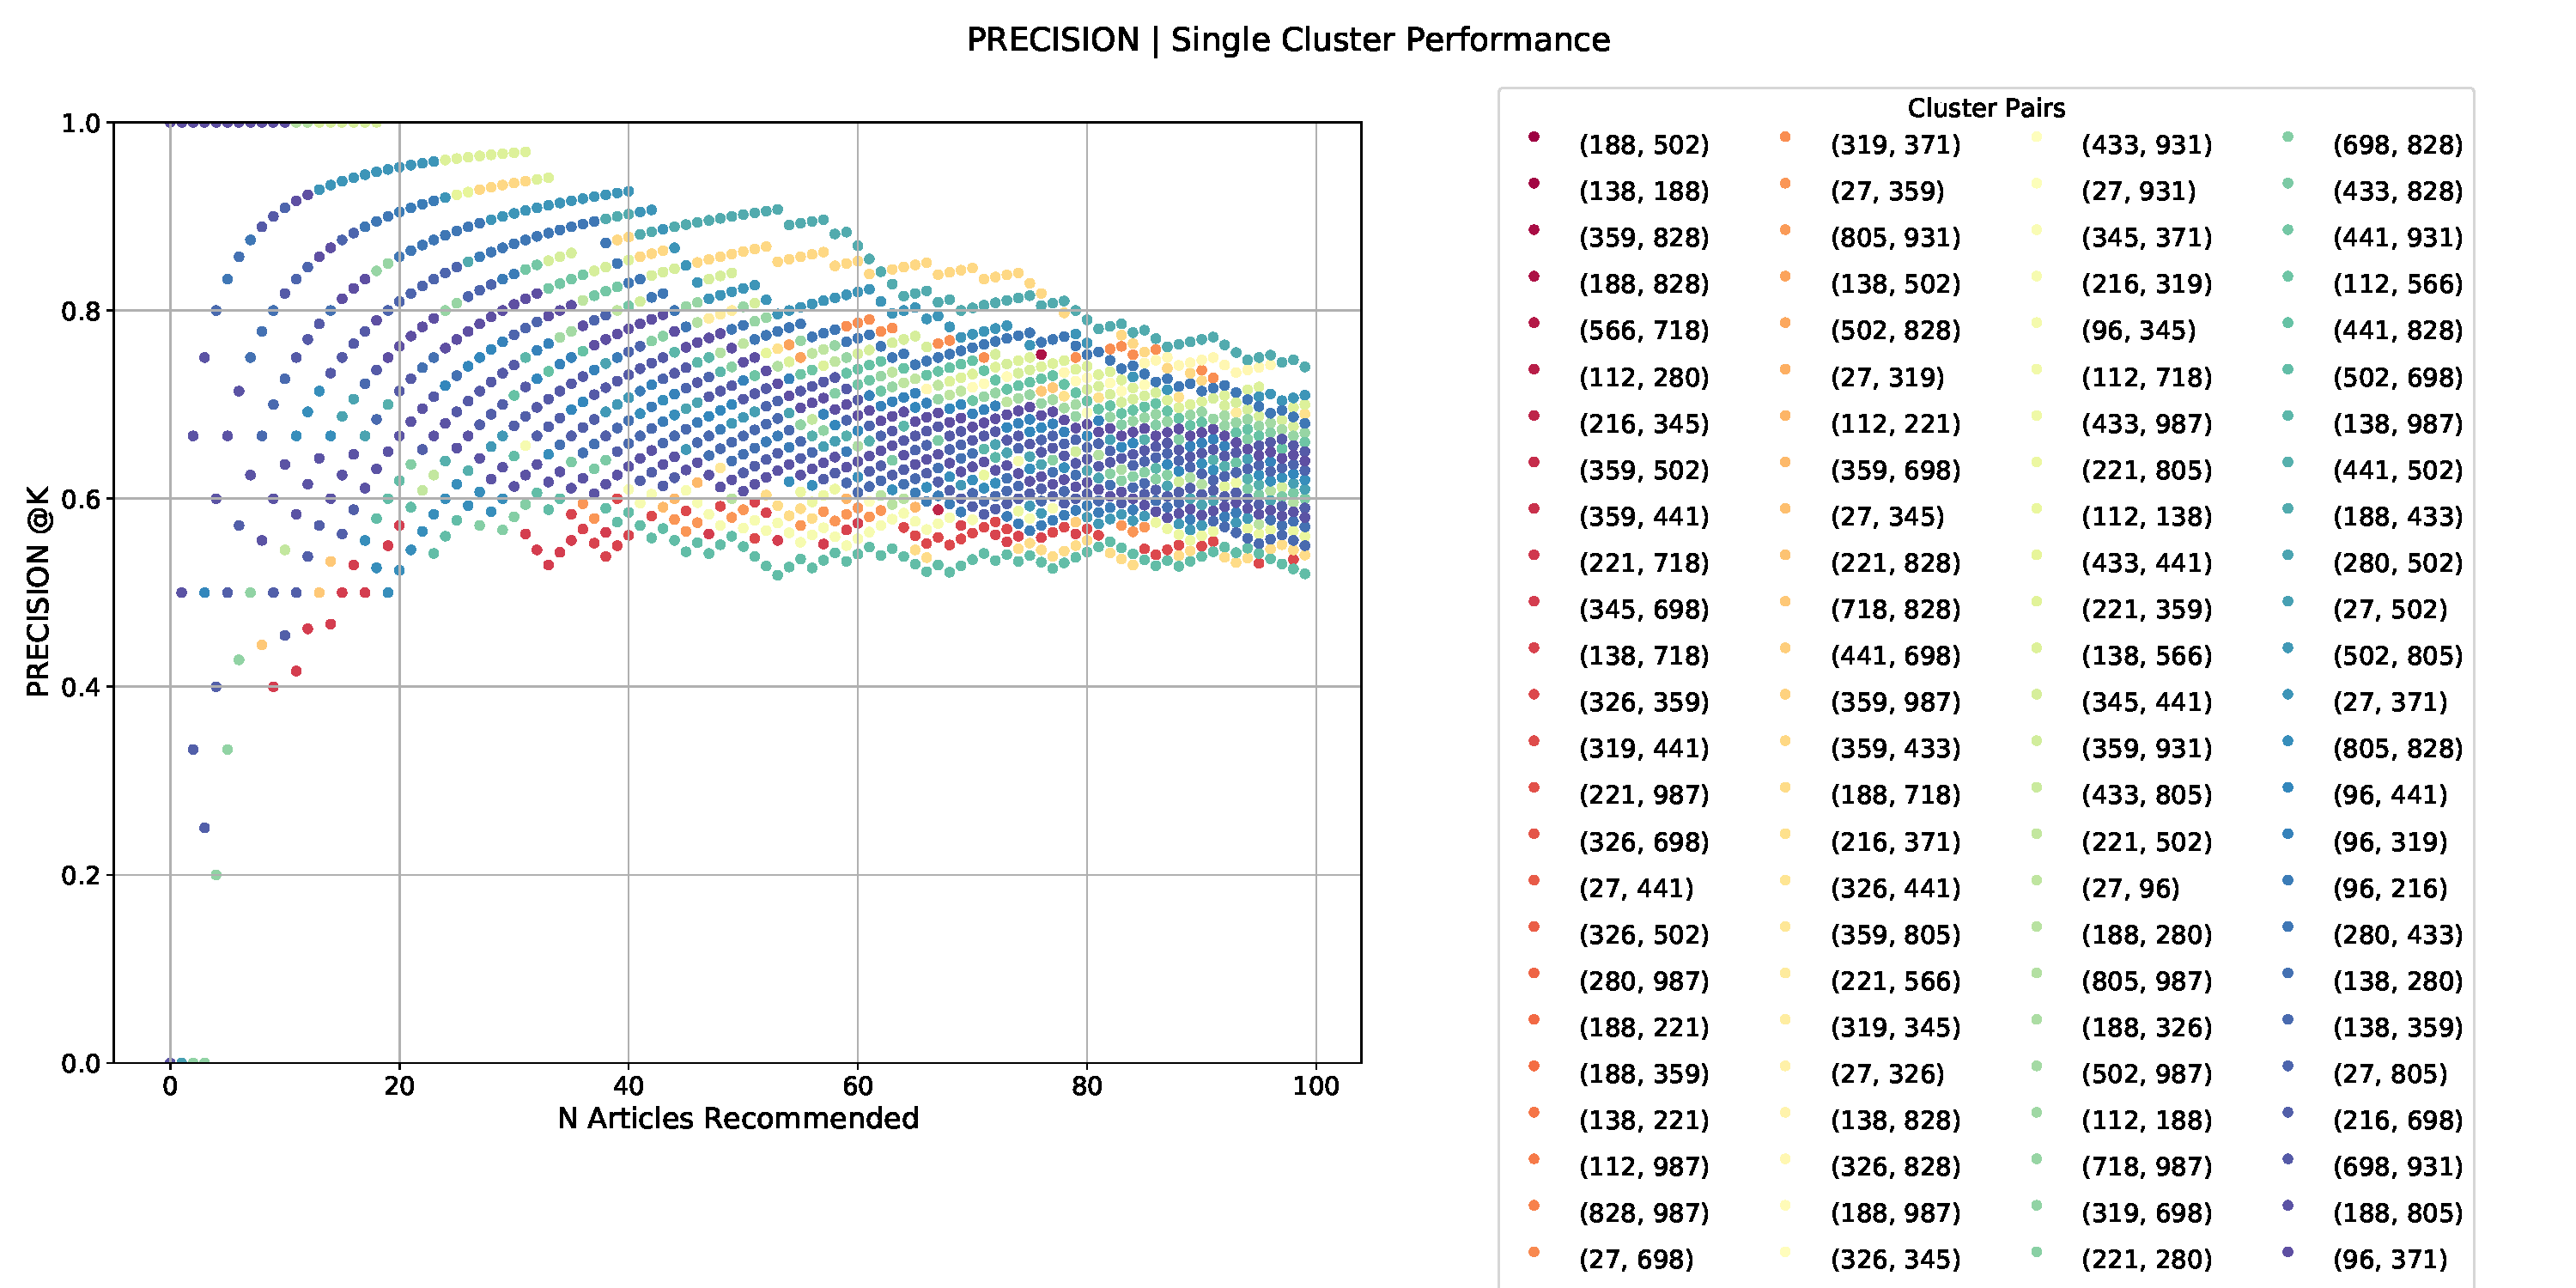
\includegraphics[width=1.0\textwidth]{Graphs/BERT/user_interaction_vs_model_performance_precision_all_cps_single_cluster.pdf}
\end{figure}
\subsection{Summary}
\begin{itemize}
    \item Better performance when only one topic/cluster is involved compared to a cluster pair setting
    \item TF-IDF has the best performance here followed by BERT and then GLOVE
\end{itemize}


\newpage
\section{Baseline 4: Varying Regularization Strength to remove Spurious Correlations}
\begin{flushleft}
\subsection{TF-IDF}
\subsubsection{Homogeneous Users}
\begin{flushleft}
For Homogeneous Users we see that a high regularization constant tends to hurt model performance, even not using a regularization constant (alpha =0) hurts precision compared to using a small regularization constant.
\end{flushleft}
\end{flushleft}
\vspace{-6ex}
\begin{figure}[H]
 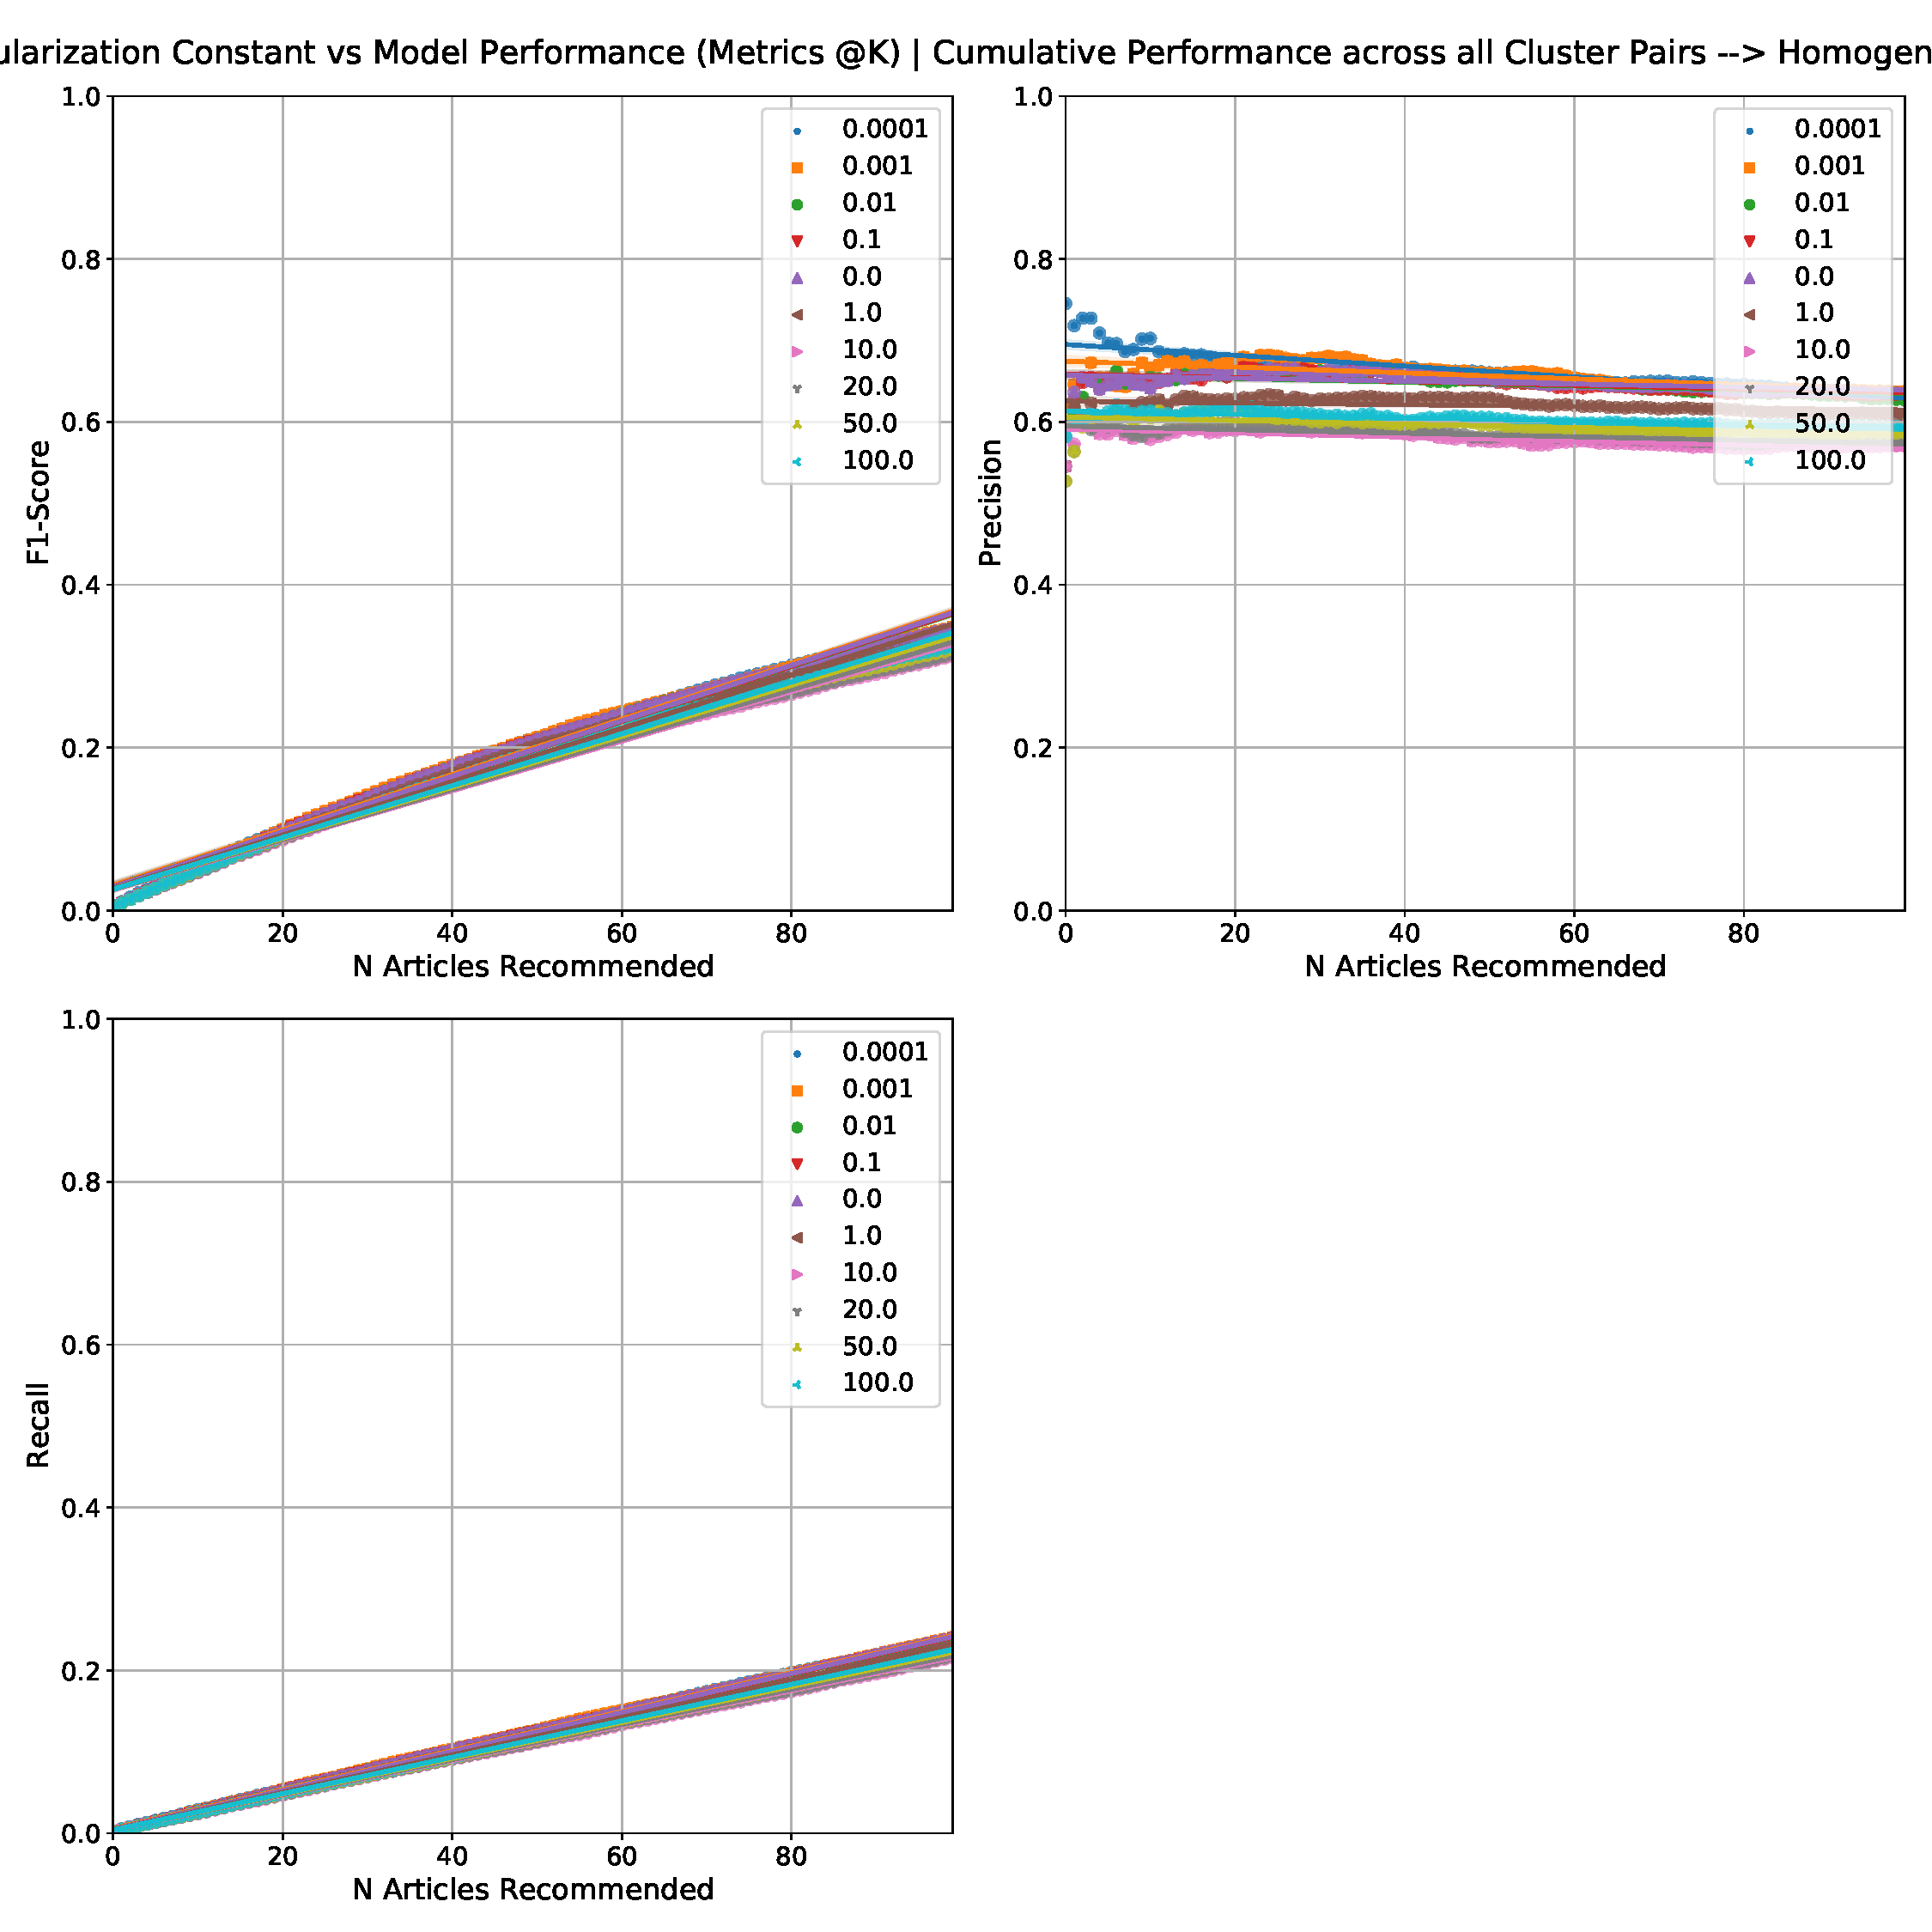
\includegraphics[width=0.7\textwidth]{Graphs/TFIDF/regularization_vs_model_performance_cumu_Homogeneous.pdf}
\end{figure}
\subsubsection{Heterogeneous Users}
\begin{flushleft}
For Heterogeneous Users on the other hand, the greater the regularization constant the better the model performs (as it can be seen across all 3 metrics), so limiting spurious correlations definitely does help in this scenario as words that overlap across stances are demoted in importance. 
\end{flushleft}
\vspace{-18ex}
\begin{figure}[H]
 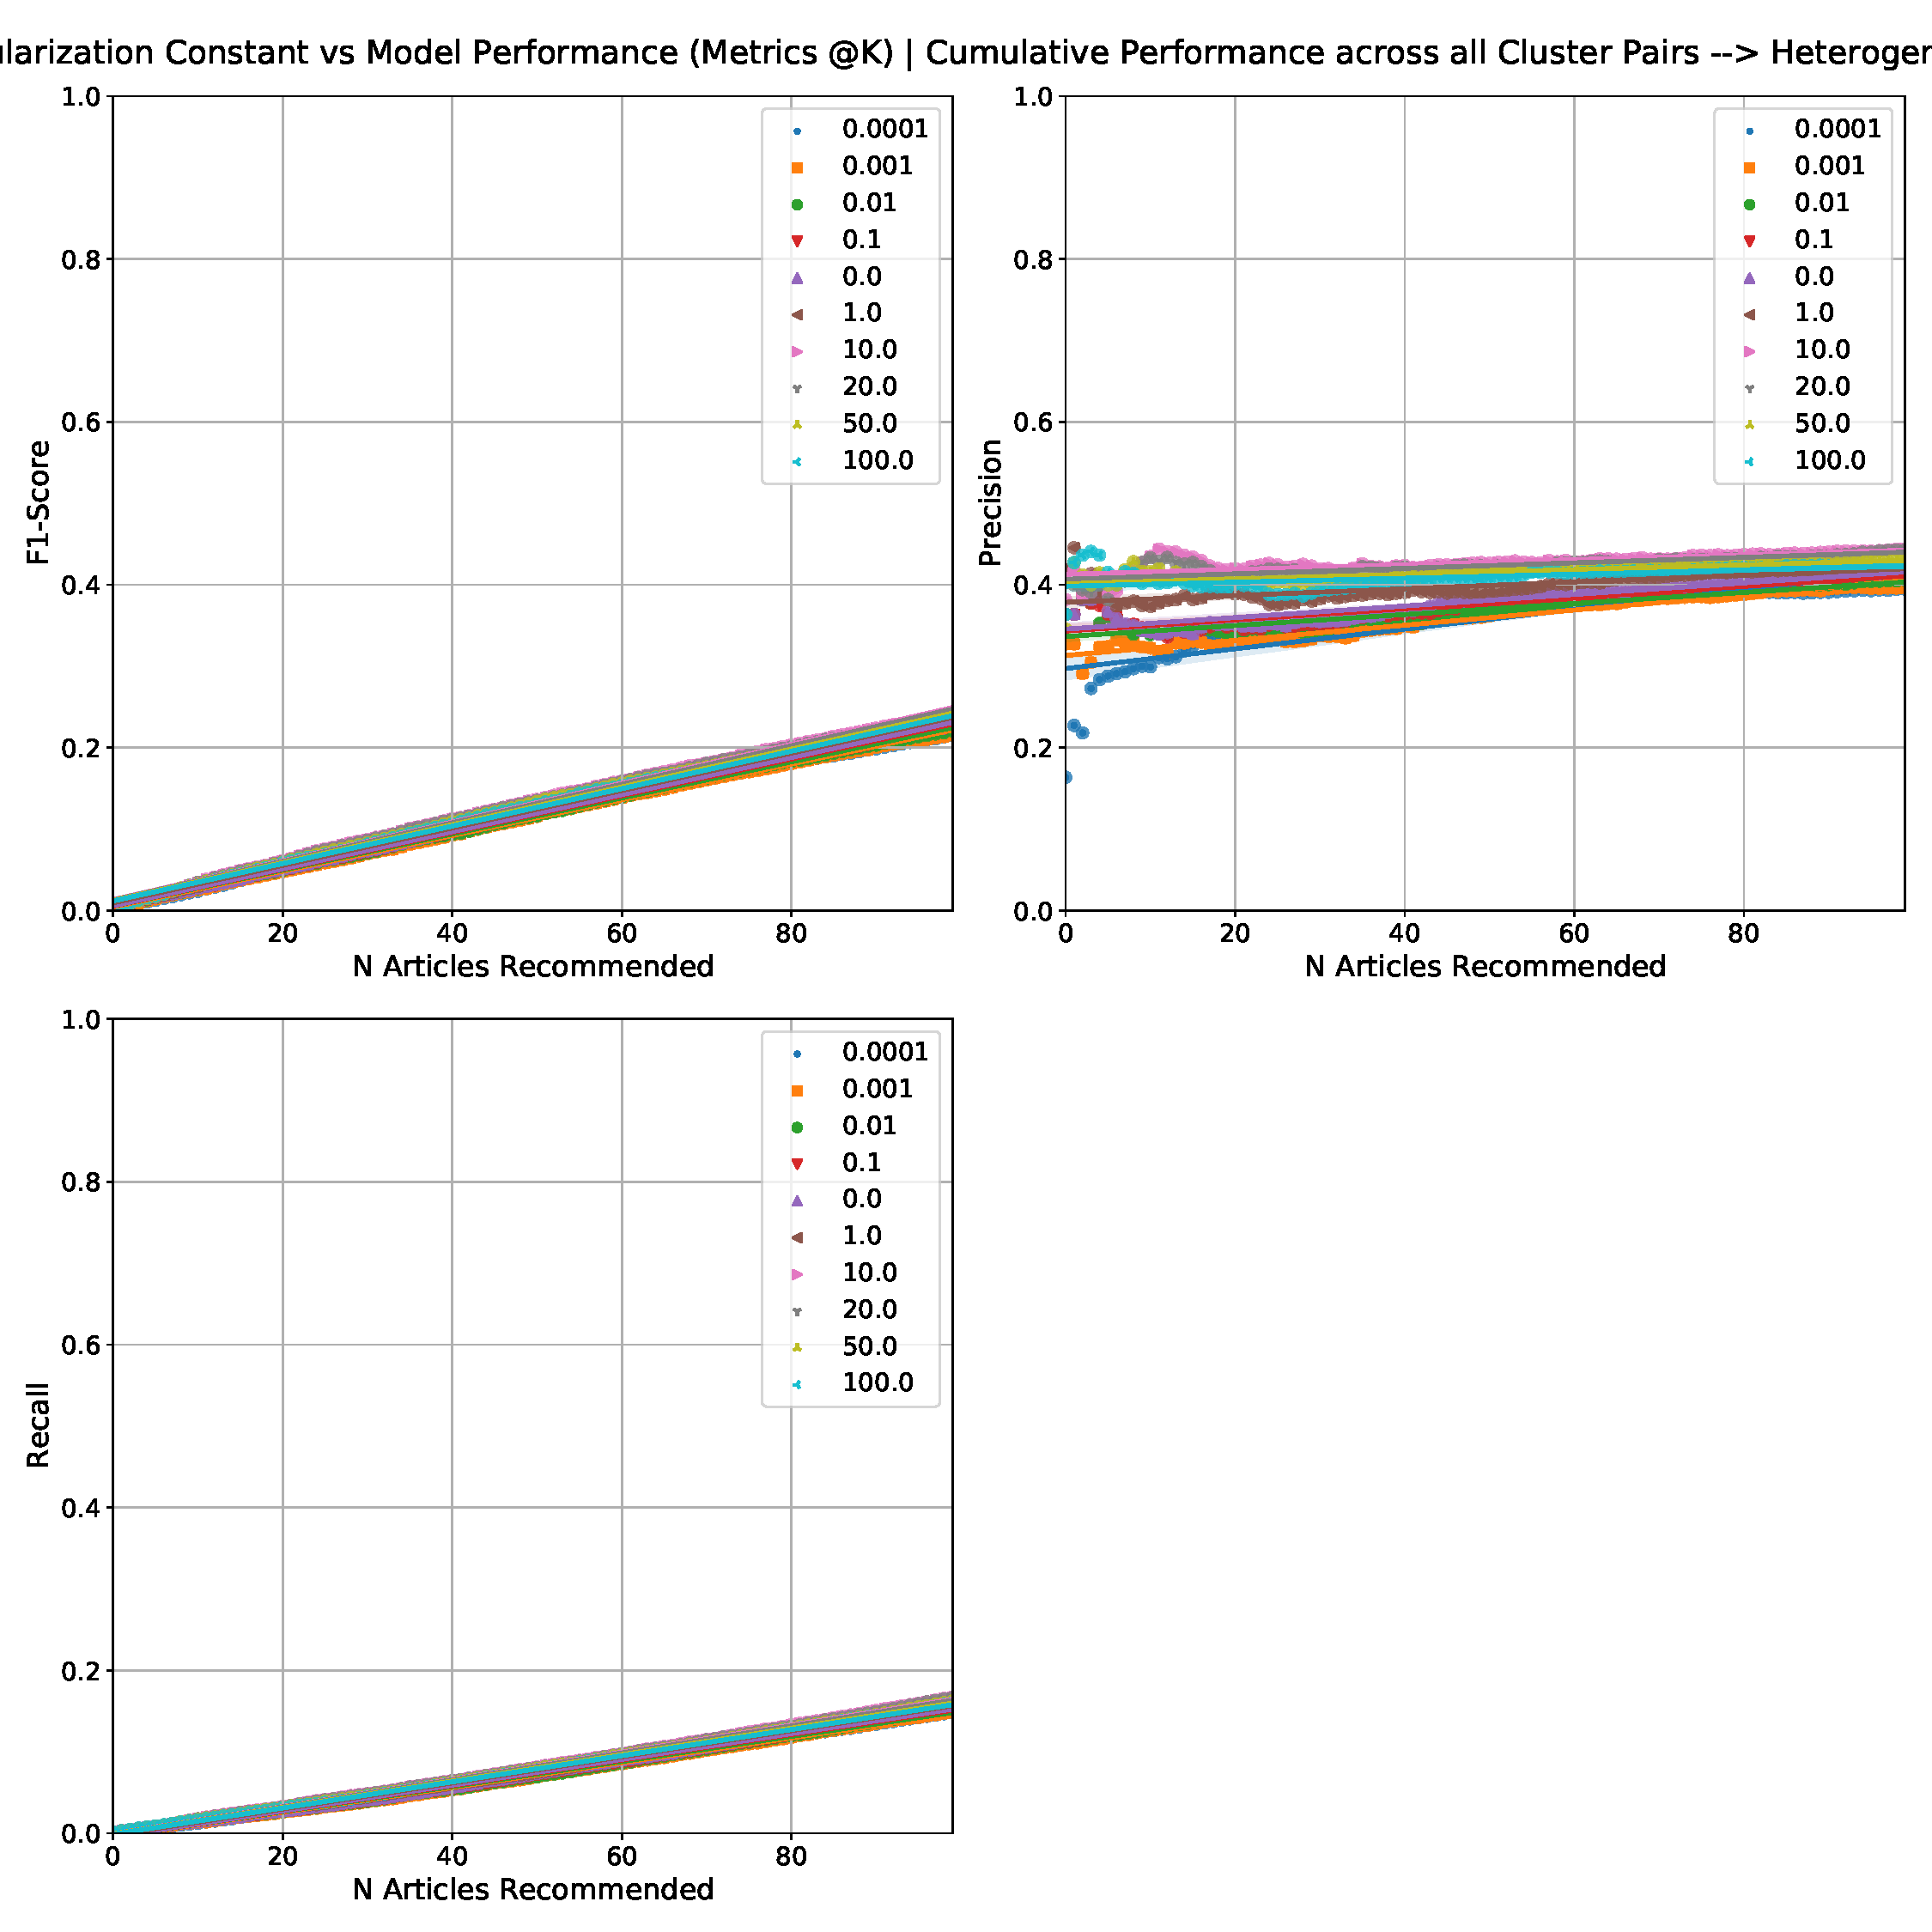
\includegraphics[width=0.7\textwidth]{Graphs/TFIDF/regularization_vs_model_performance_cumu_Heterogeneous.pdf}
\end{figure}
\subsection{Glove}
\subsubsection{Homogeneous Users}
\begin{flushleft}
For Homogeneous Users we see that a high regularization constant tends to keep the precision at a more constant rate compared to a smaller regularization constant but has lower values initially.
\end{flushleft}
\vspace{-1ex}
\begin{figure}[H]
 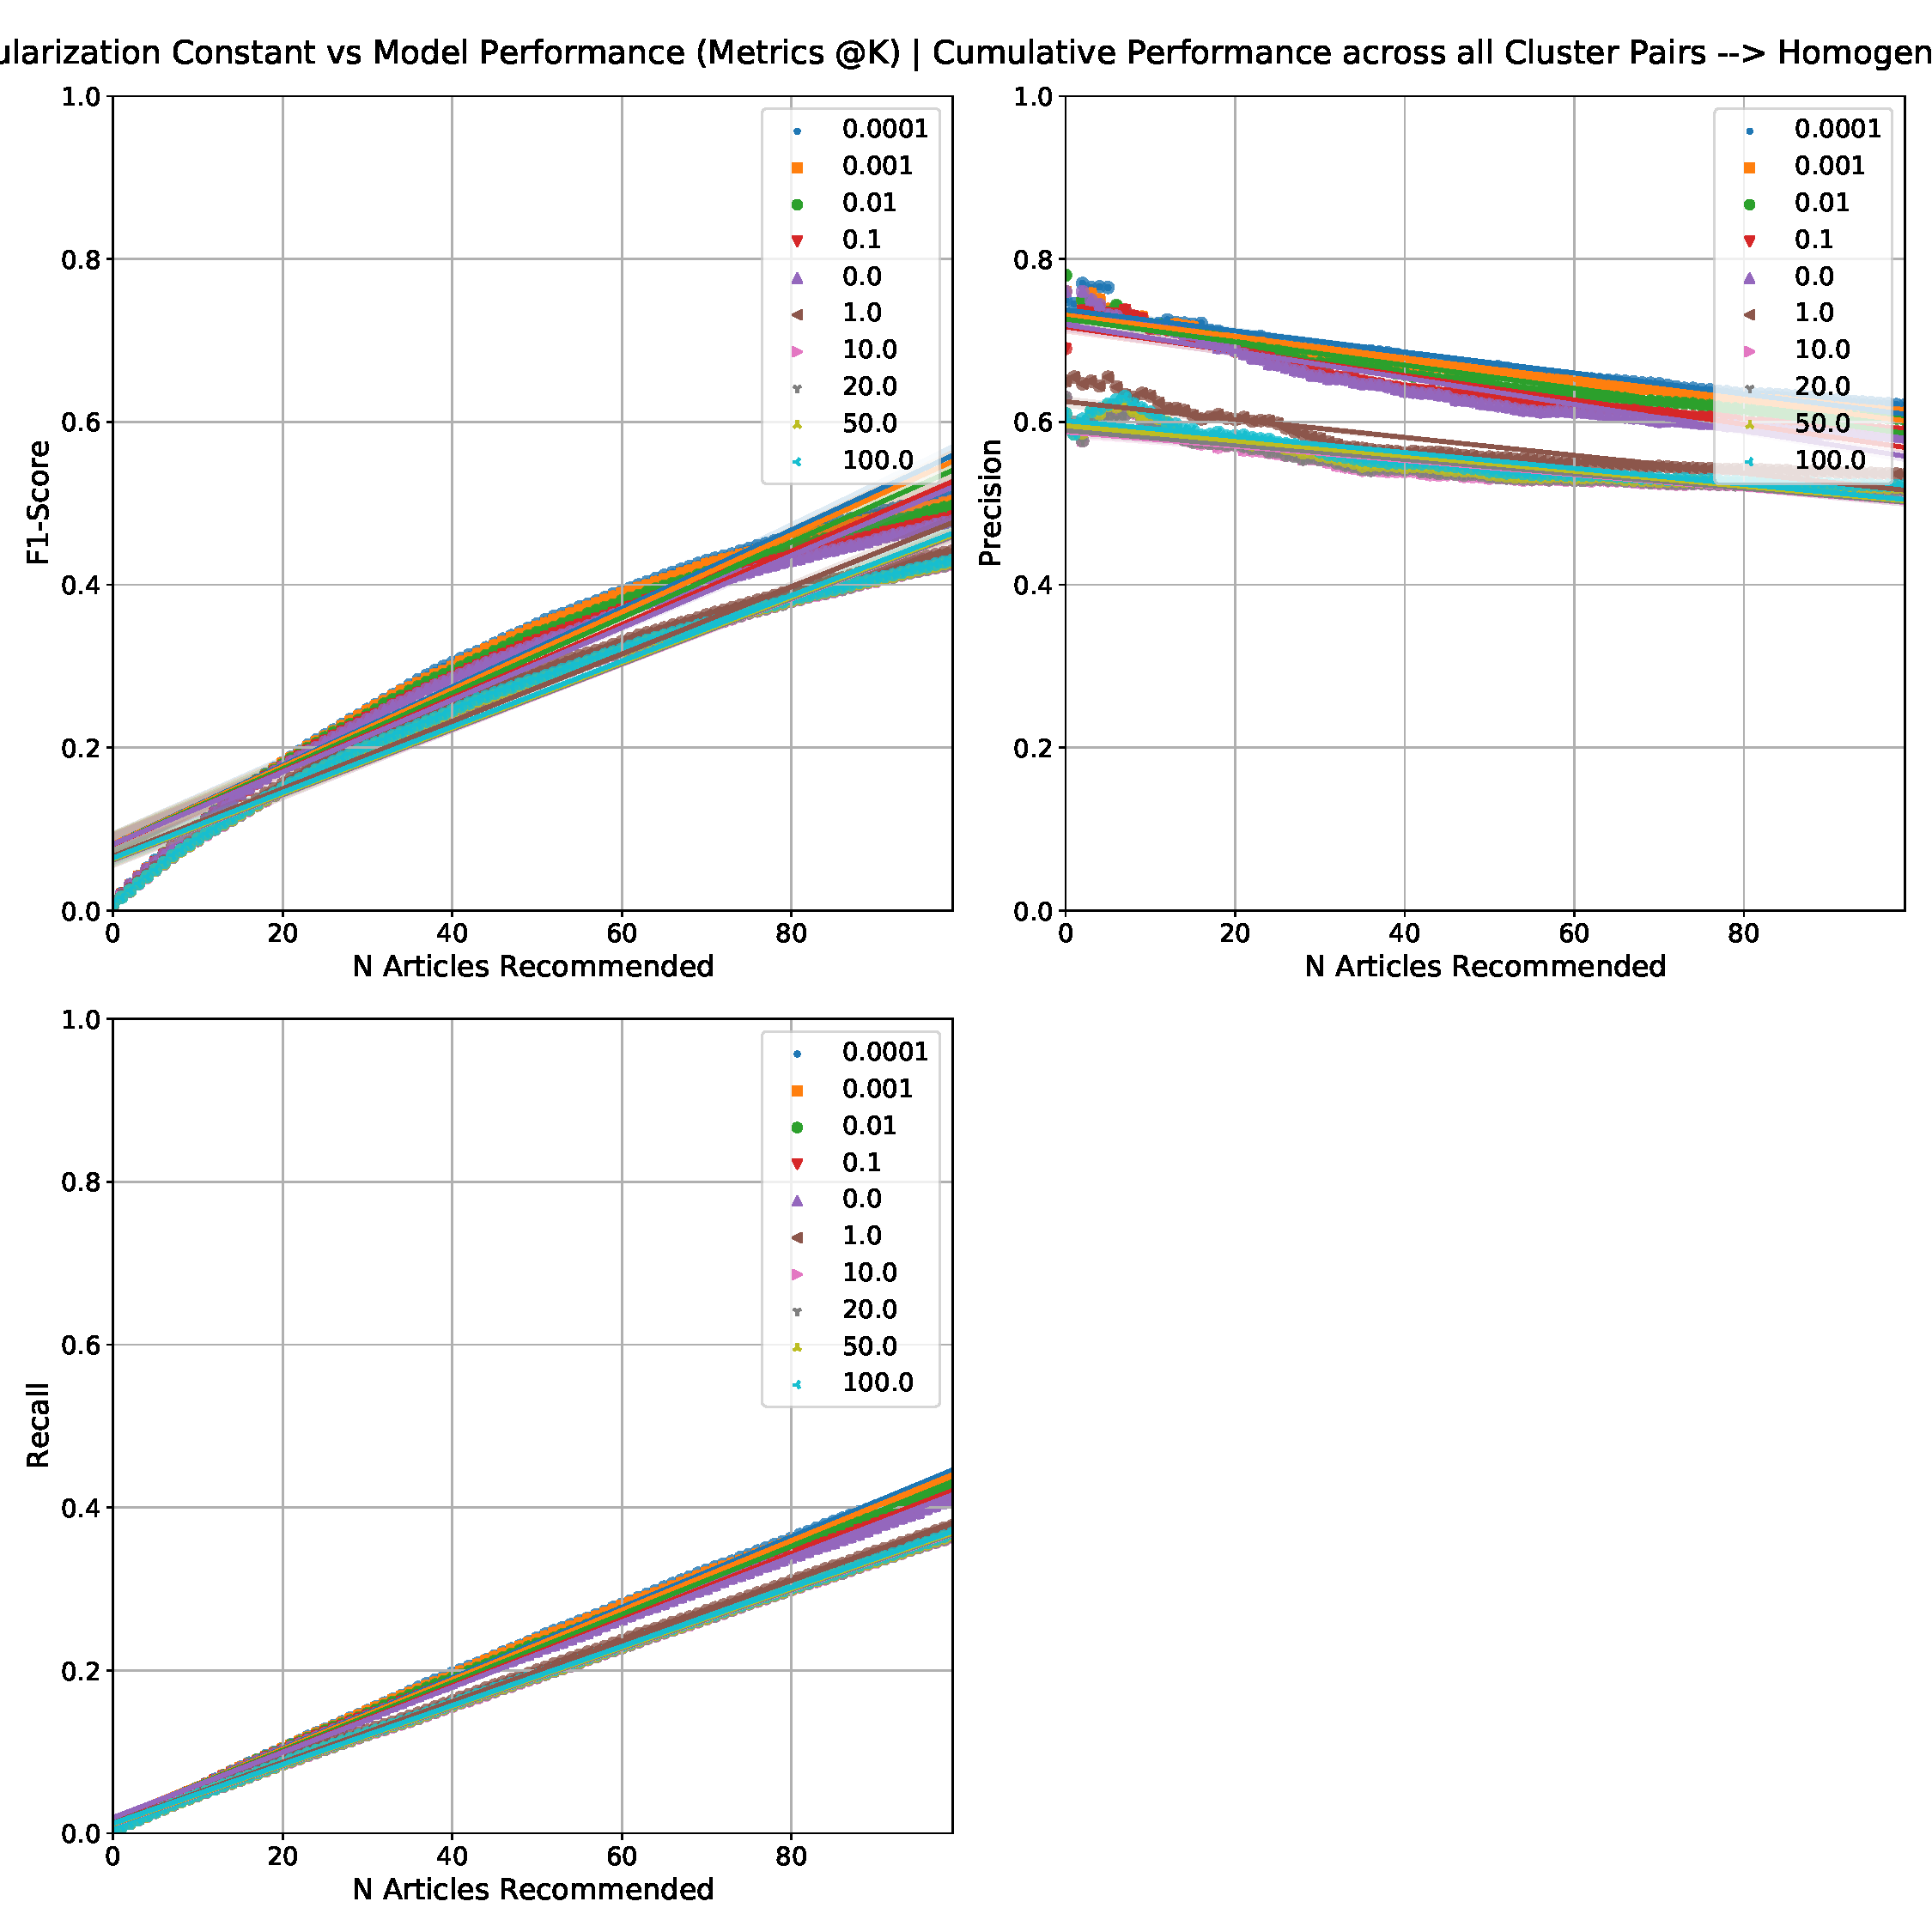
\includegraphics[width=0.7\textwidth]{Graphs/GLOVE/regularization_vs_model_performance_cumu_Homogeneous.pdf}
\end{figure}
\vspace{-3ex}
\subsubsection{Heterogeneous Users}
\begin{flushleft}
For Heterogeneous Users on the other hand, higher regularization constant values improves precision over lower regularization constant values and the precision seems to be increase at a more constant rate compared to lower values.
\end{flushleft}
\vspace{-1ex}
\begin{figure}[H]
 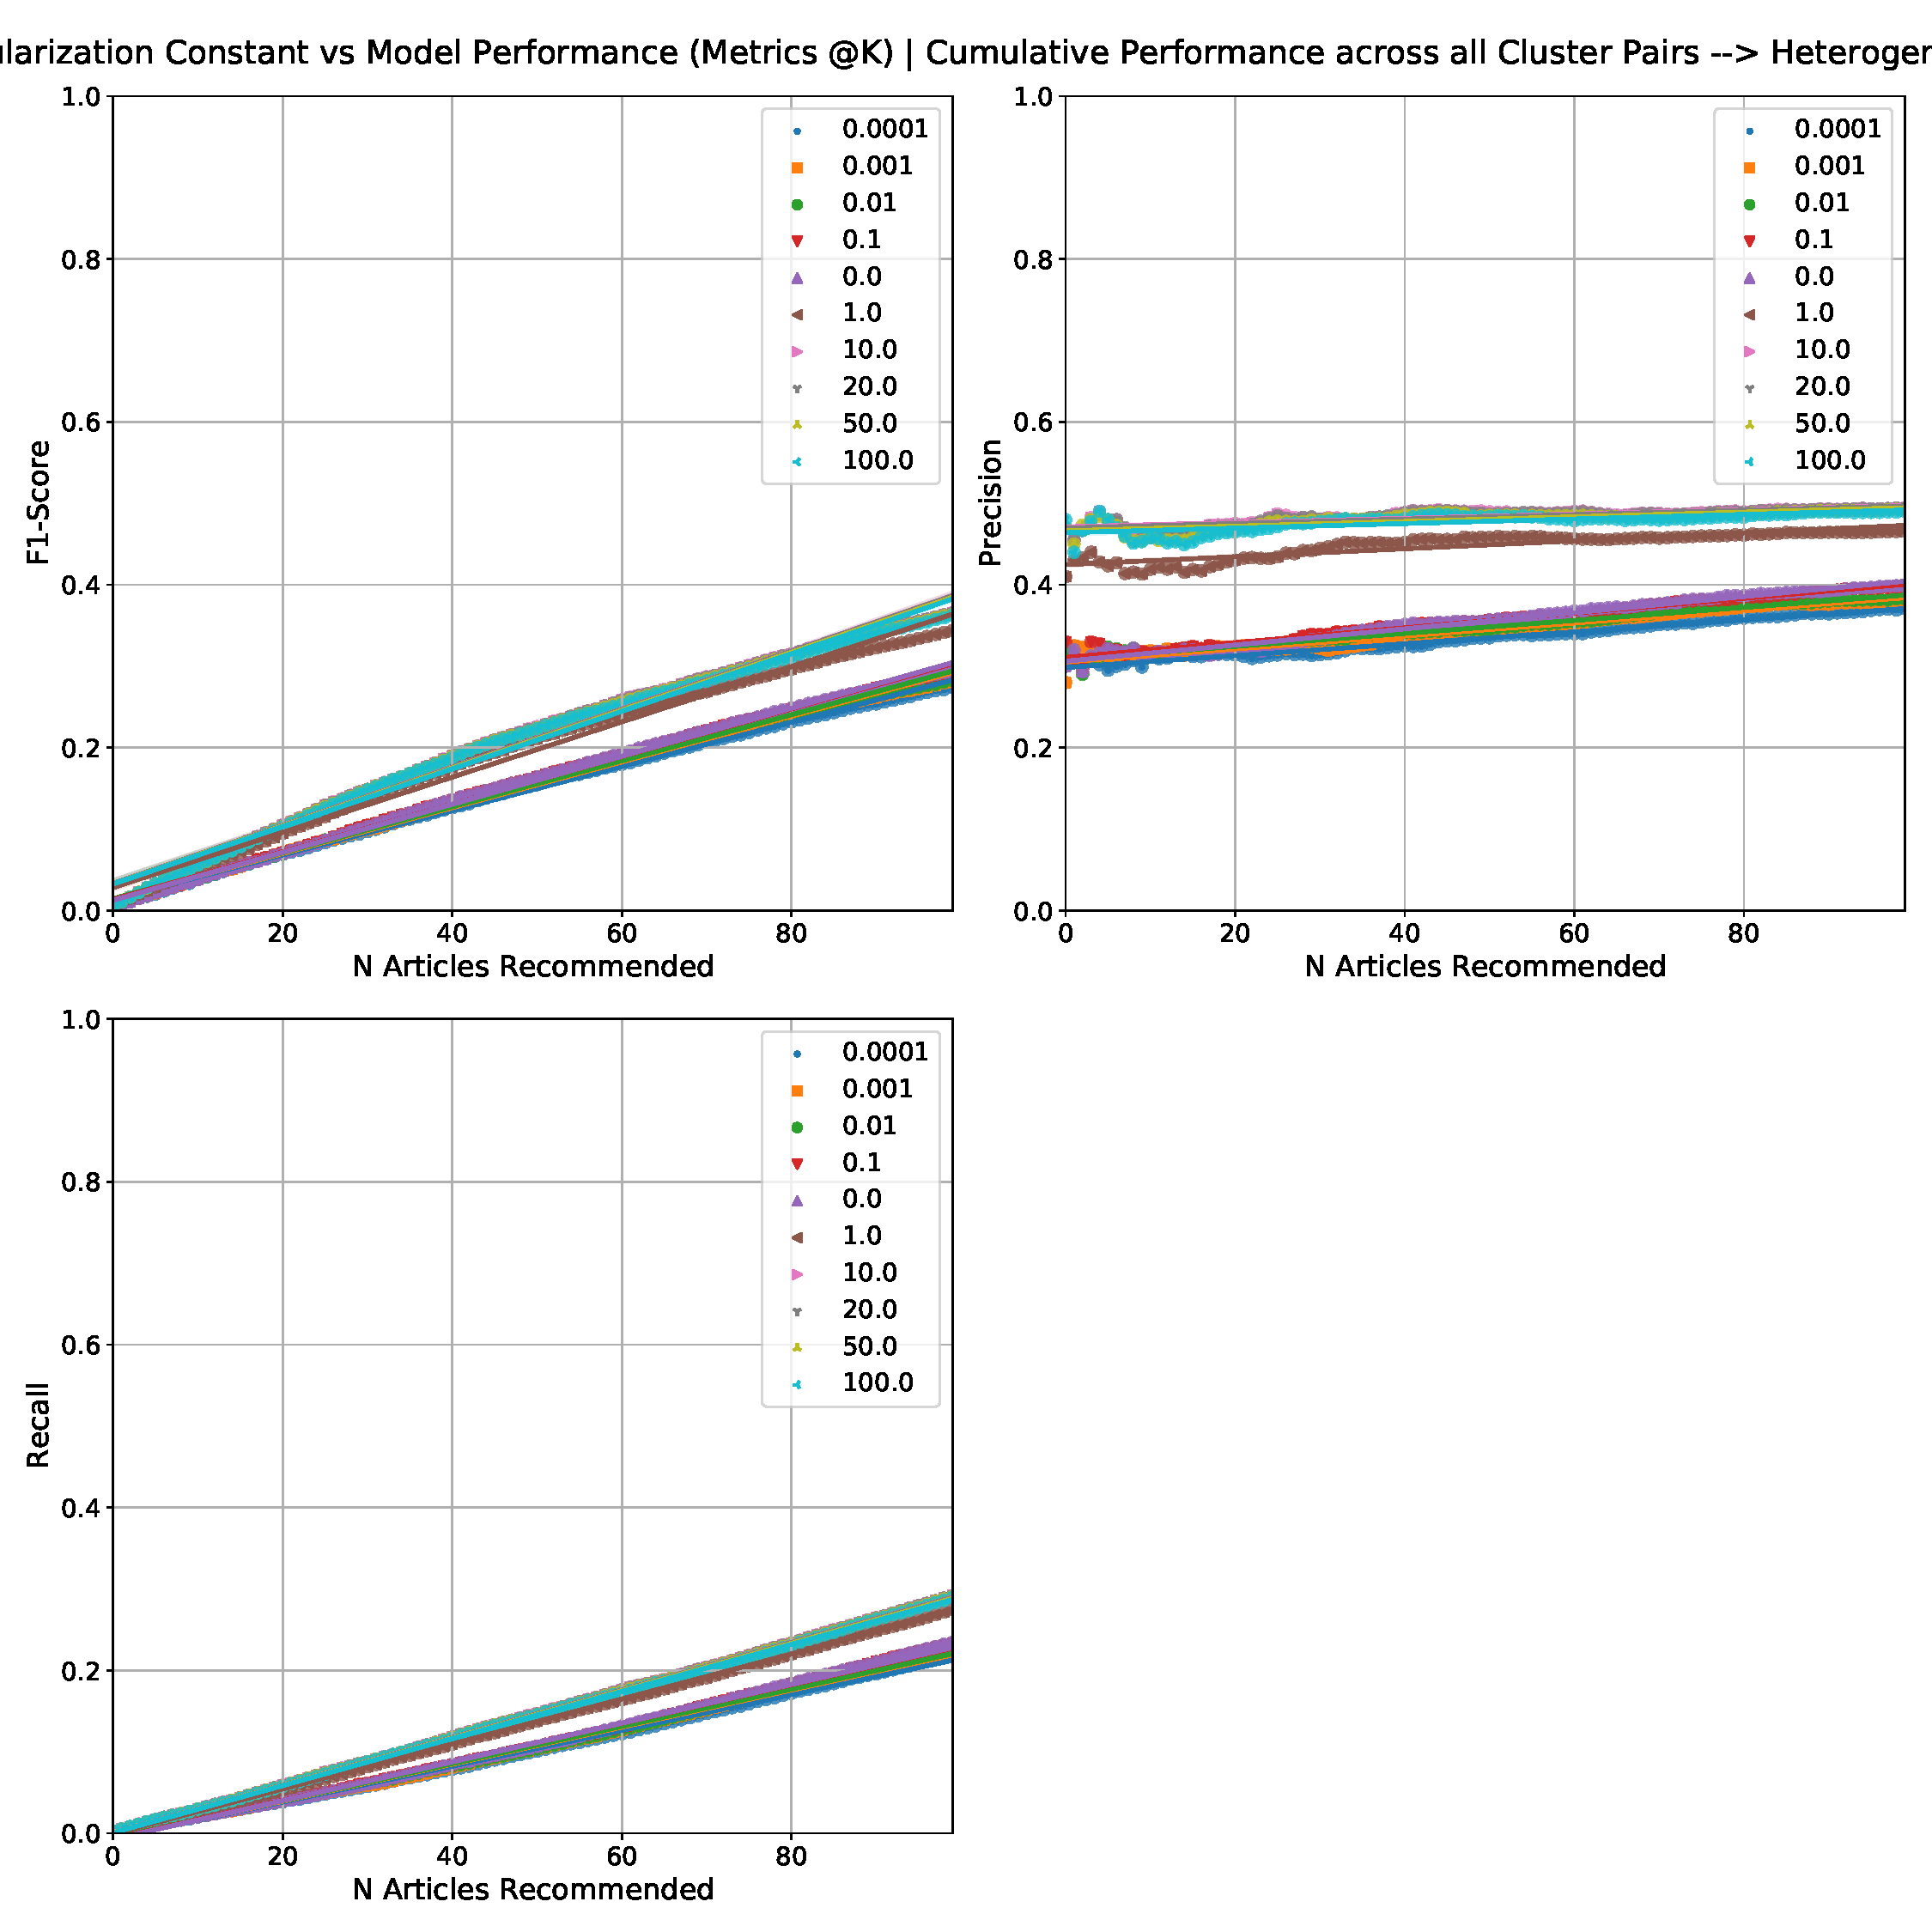
\includegraphics[width=0.7\textwidth]{Graphs/GLOVE/regularization_vs_model_performance_cumu_Heterogeneous.pdf}
\end{figure}
\subsection{BERT}
\subsubsection{Homogeneous Users}
\begin{flushleft}
For Homogeneous Users we see that lower regularization values have high precision compared to higher constant values and we also observe that the precision for the initial interactions are much higher compared to when using TFIDF and GLOVE representations
\end{flushleft}
\begin{figure}[H]
 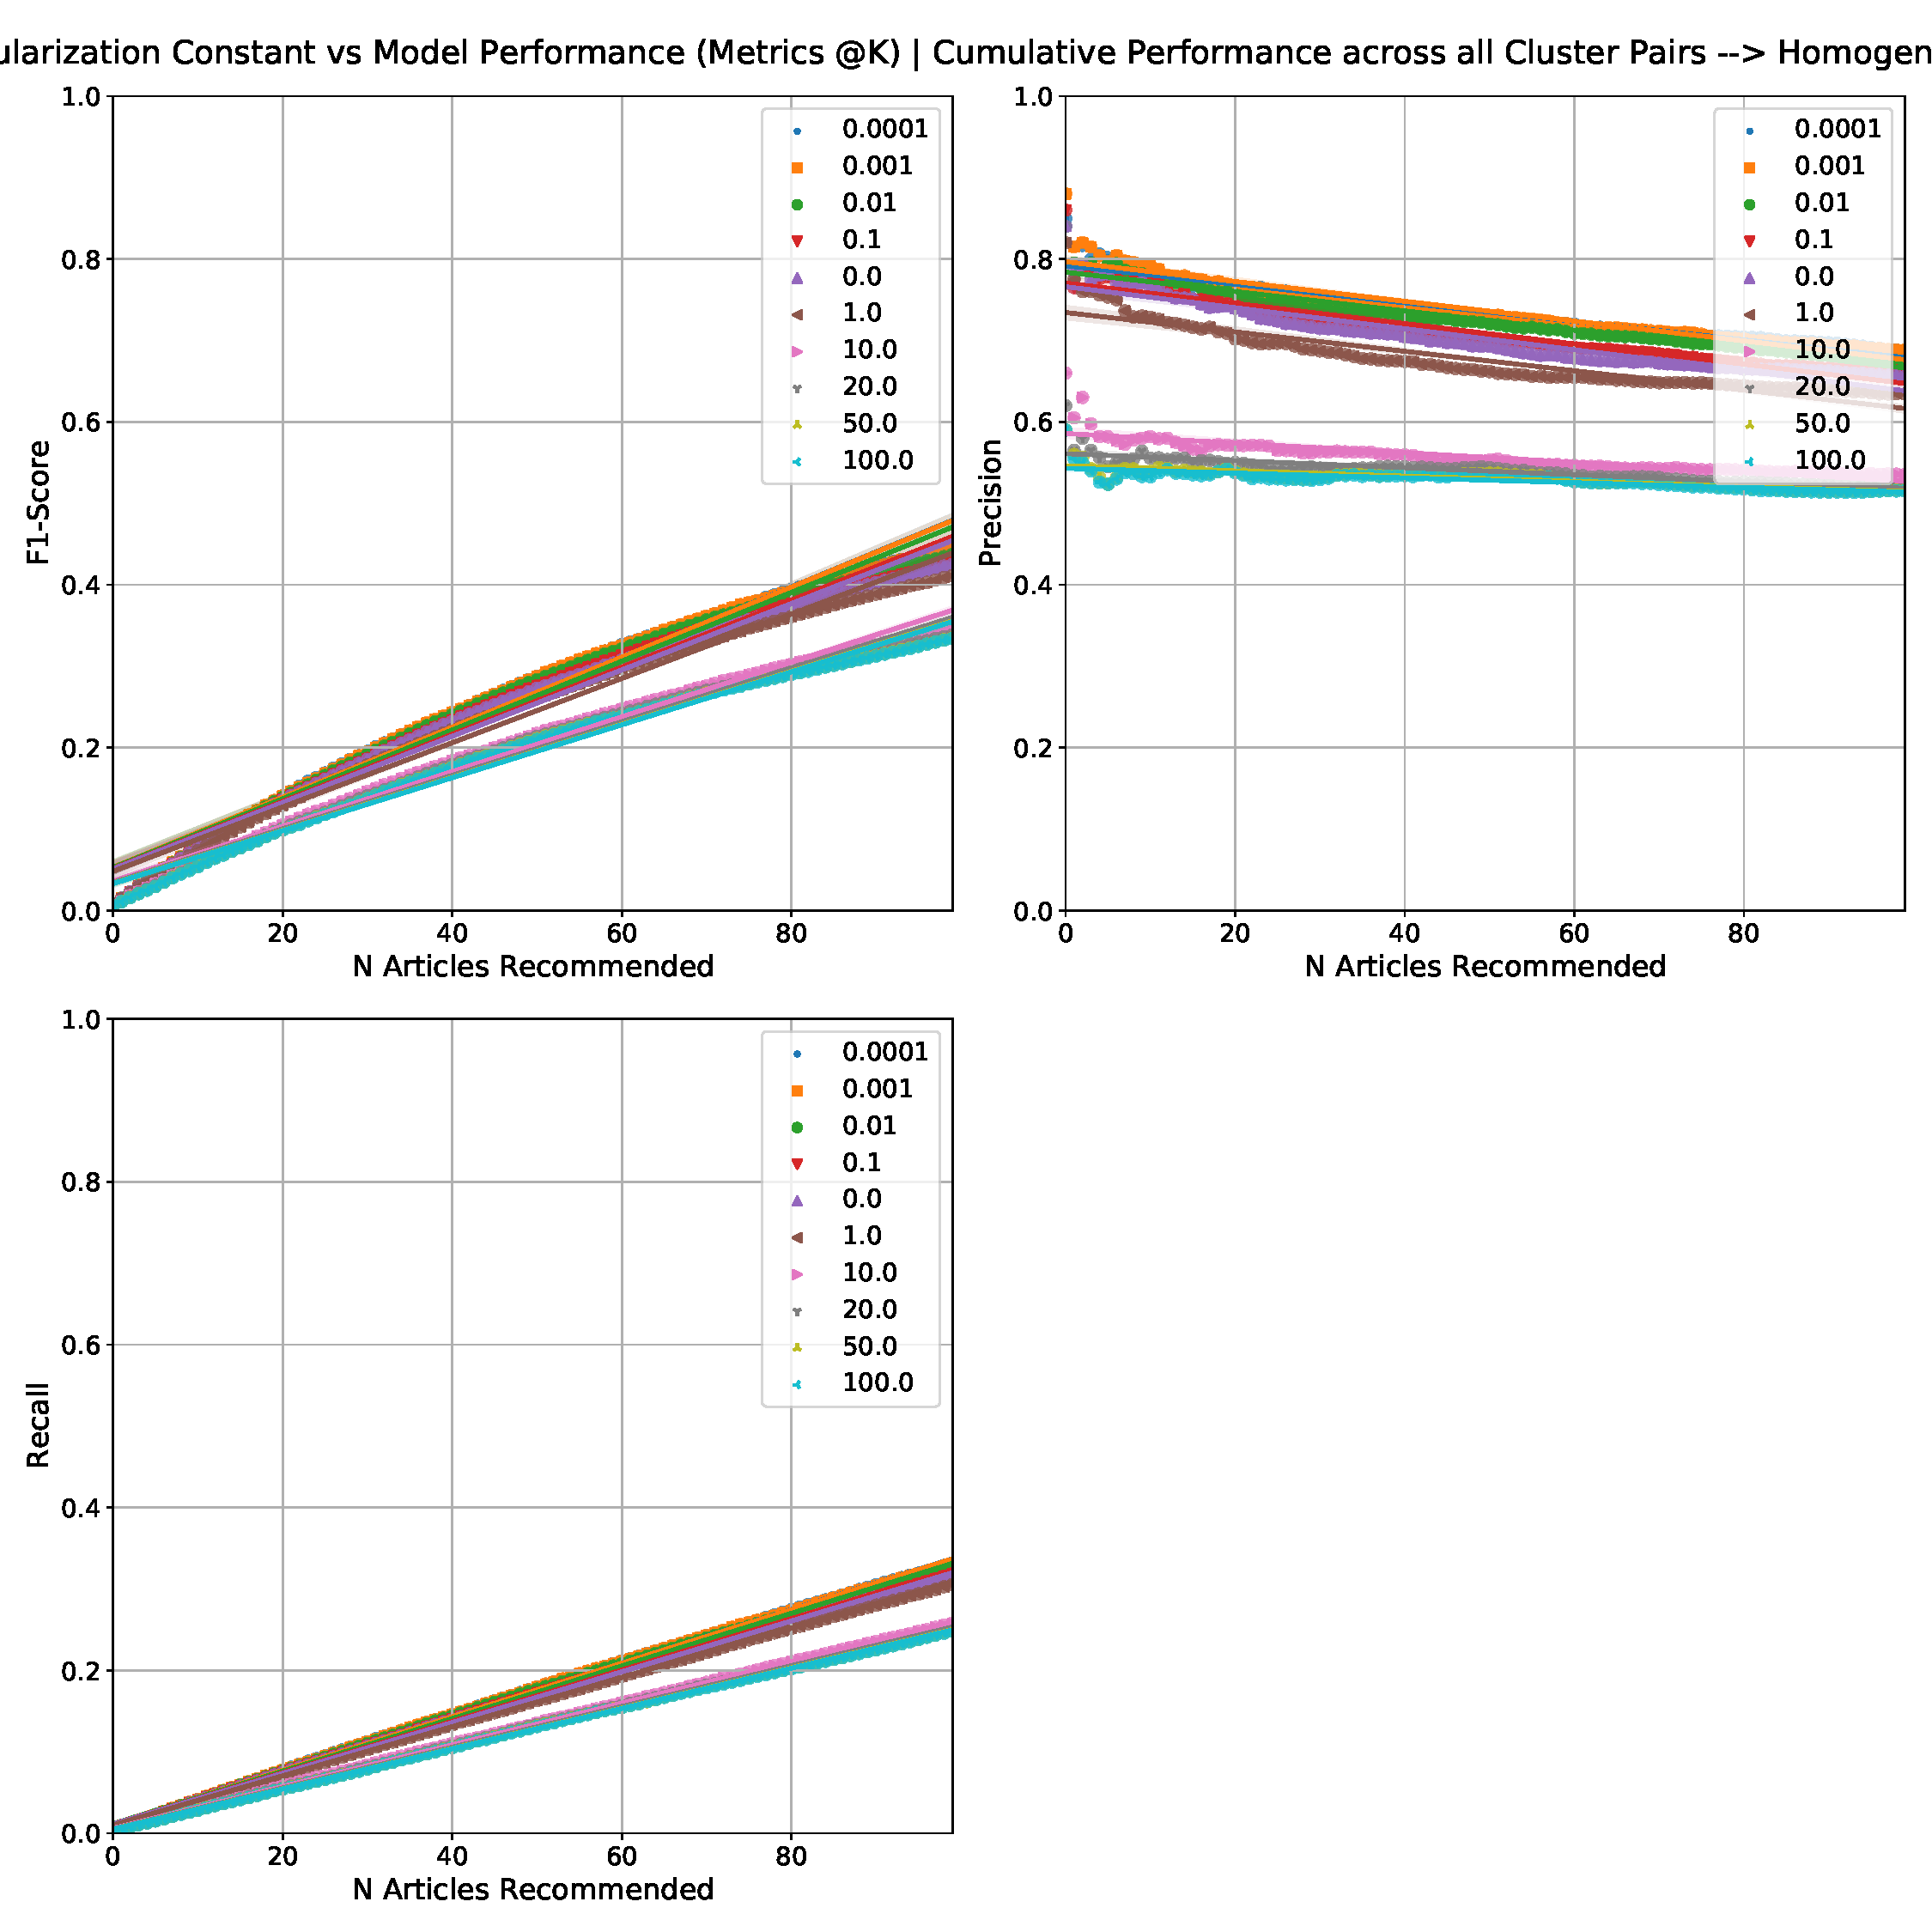
\includegraphics[width=0.7\textwidth]{Graphs/BERT/regularization_vs_model_performance_cumu_Homogeneous.pdf}
\end{figure}
\subsubsection{Heterogeneous Users}
\begin{flushleft}
For Heterogeneous Users on the other hand, higher regularization constant values improves precision over lower regularization constant values and the precision seems to be increase at a more constant rate compared to lower values. We also observe that both GLOVE and TFIDF Representations tend to have a higher precision compared to BERT for lower regularization values.
\end{flushleft}
\vspace{-1ex}
\begin{figure}[H]
 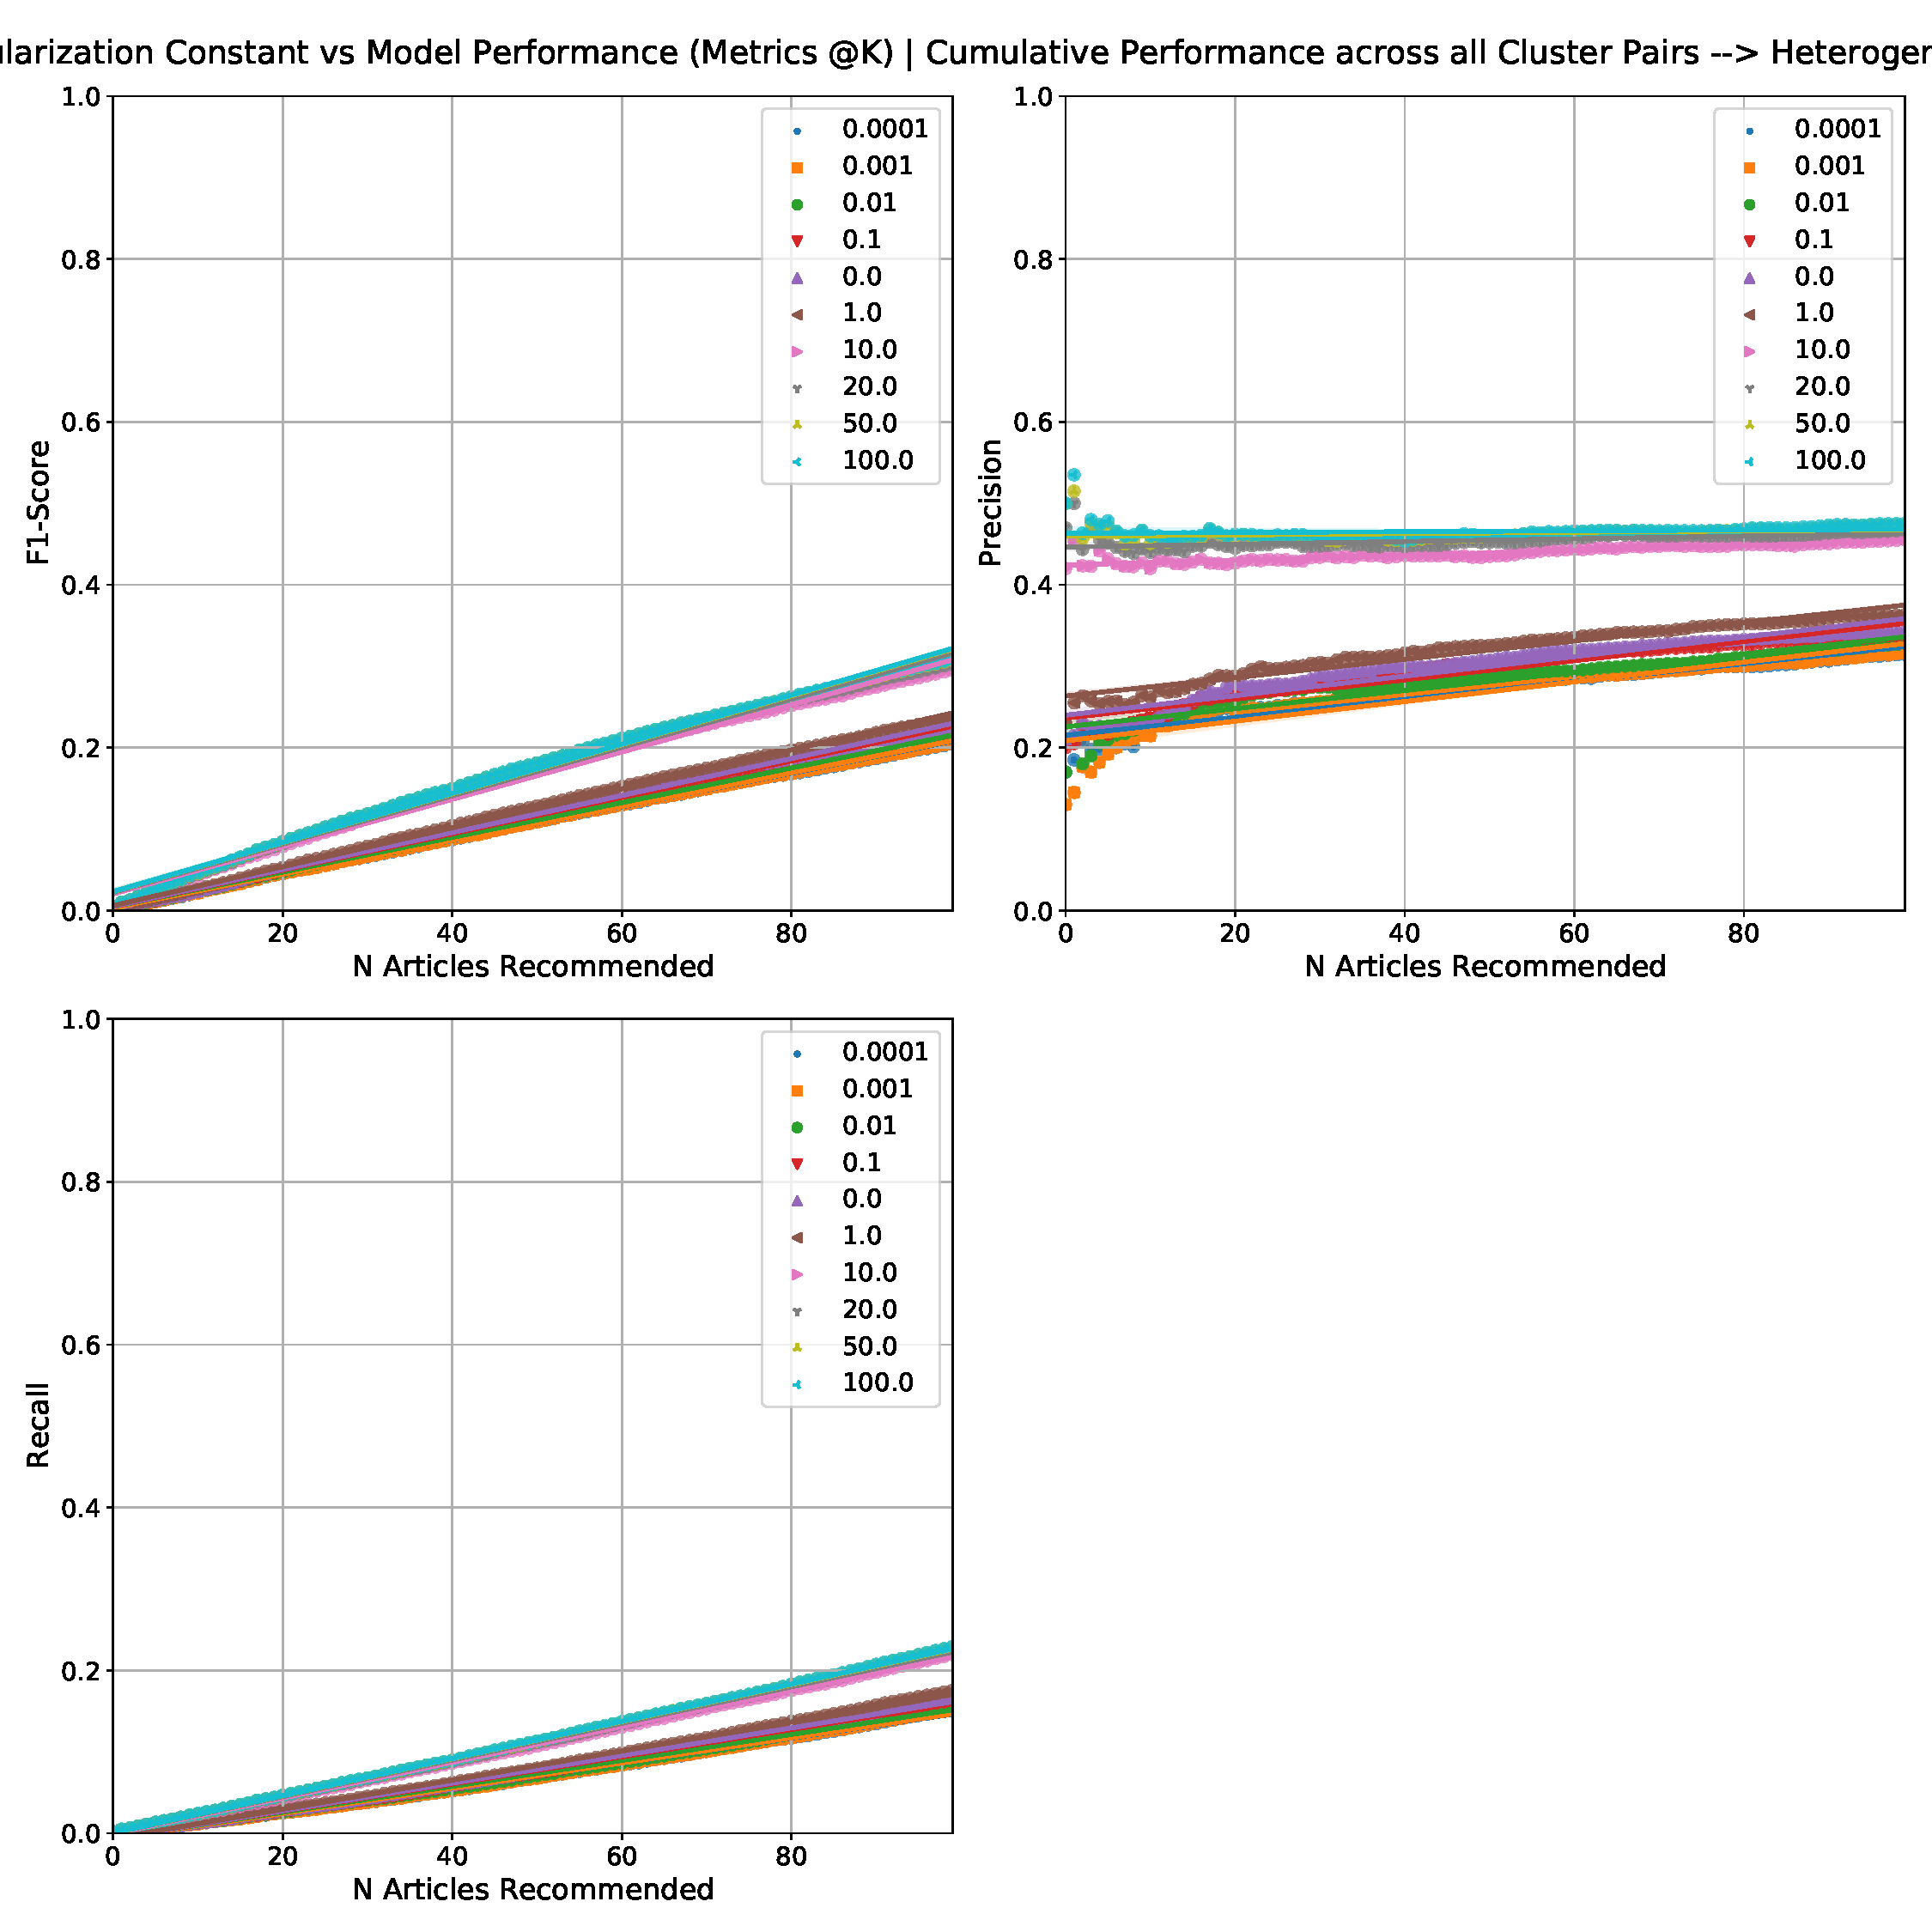
\includegraphics[width=0.7\textwidth]{Graphs/BERT/regularization_vs_model_performance_cumu_Heterogeneous.pdf}
\end{figure}
\subsection{Summary}
\begin{itemize}
    \item TF-IDF is not affected greatly by using regularization constants for the Homogeneous users compared to GLOVE and BERT representations
    \item BERT representations have higher initial precision for Homogeneous users compared to TFIDF and GLOVE with low regularization constant values
    \item GLOVE representations with high regularization constant values seems to be performing the best for Heterogeneous Users, followed by BERT (with only high regularization values)
\end{itemize}


\newpage
\section{Baseline 5: Learning Rate vs Model Performance}
\begin{flushleft}
We want to measure the effect of using different learning rates to see which leads to better convergence when max-iterations are set to 1000.
\end{flushleft}
\subsection{TF-IDF}
\subsubsection{Homogeneous Users :}
\begin{figure}[H]
 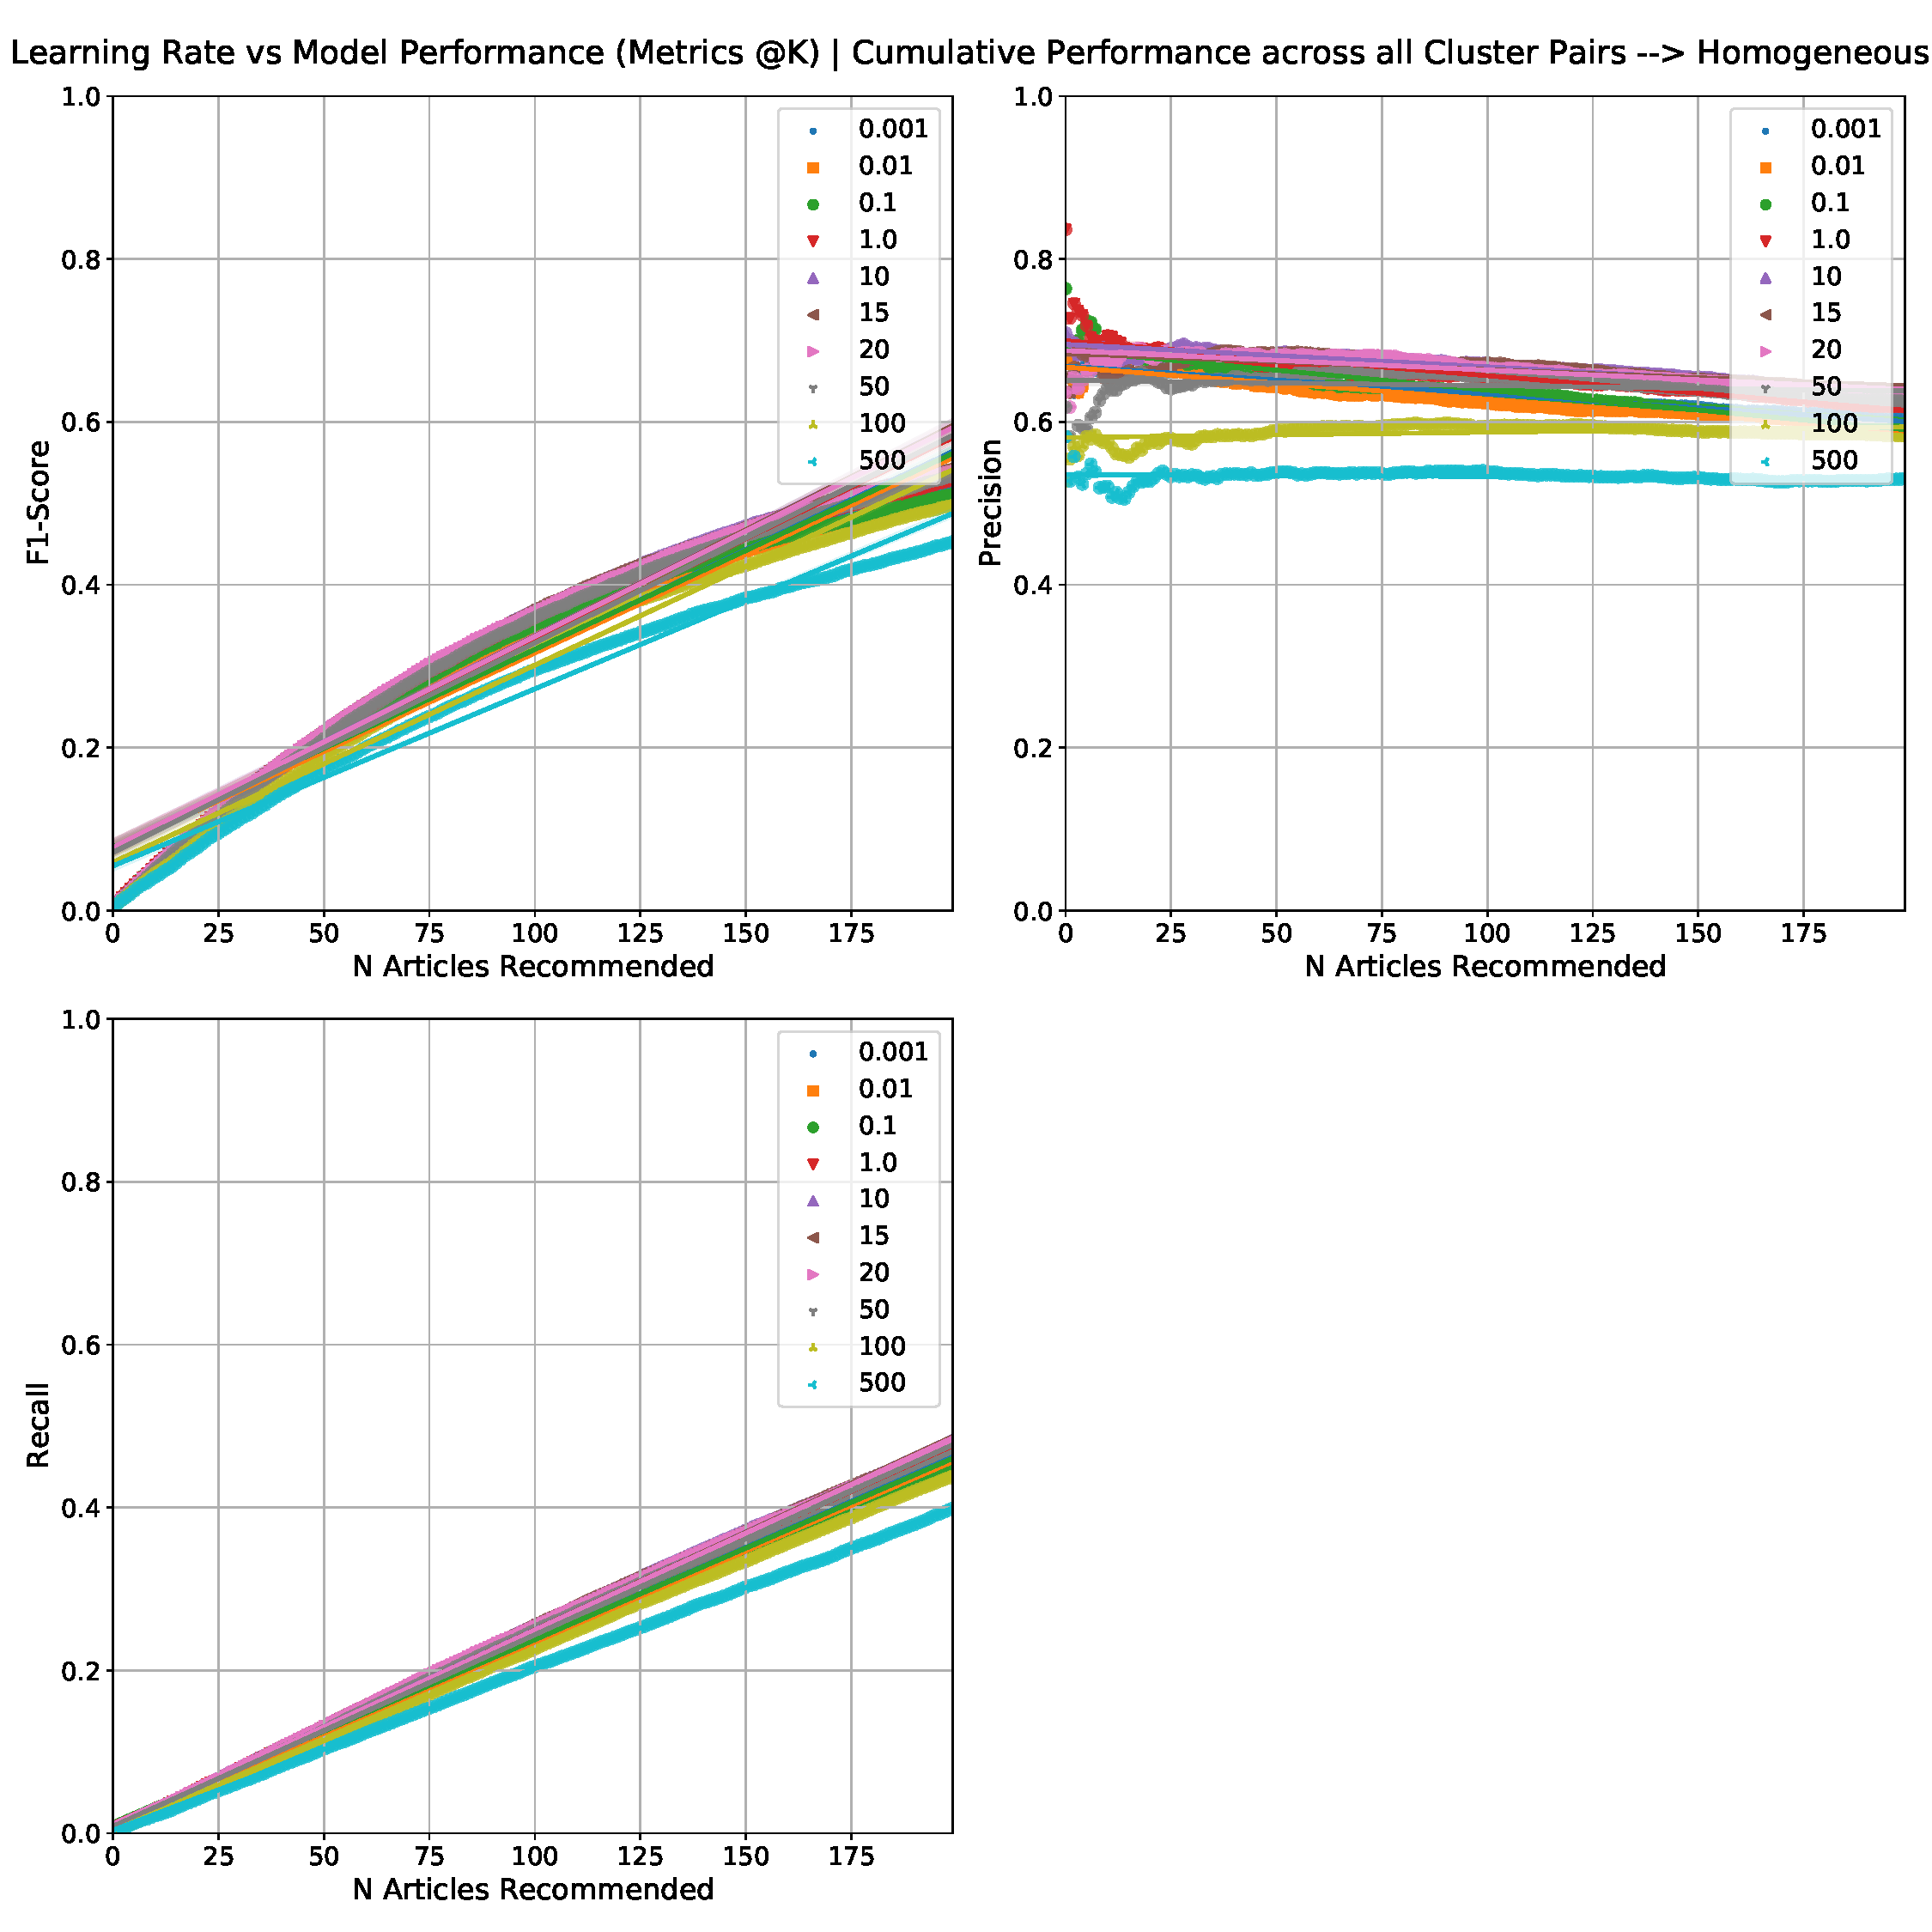
\includegraphics[width=0.6\textwidth]{Graphs/TFIDF/lr_vs_model_performance_cumu_Homogeneous.pdf}
\end{figure}
\subsubsection{Heterogeneous Users :}
\begin{figure}[H]
 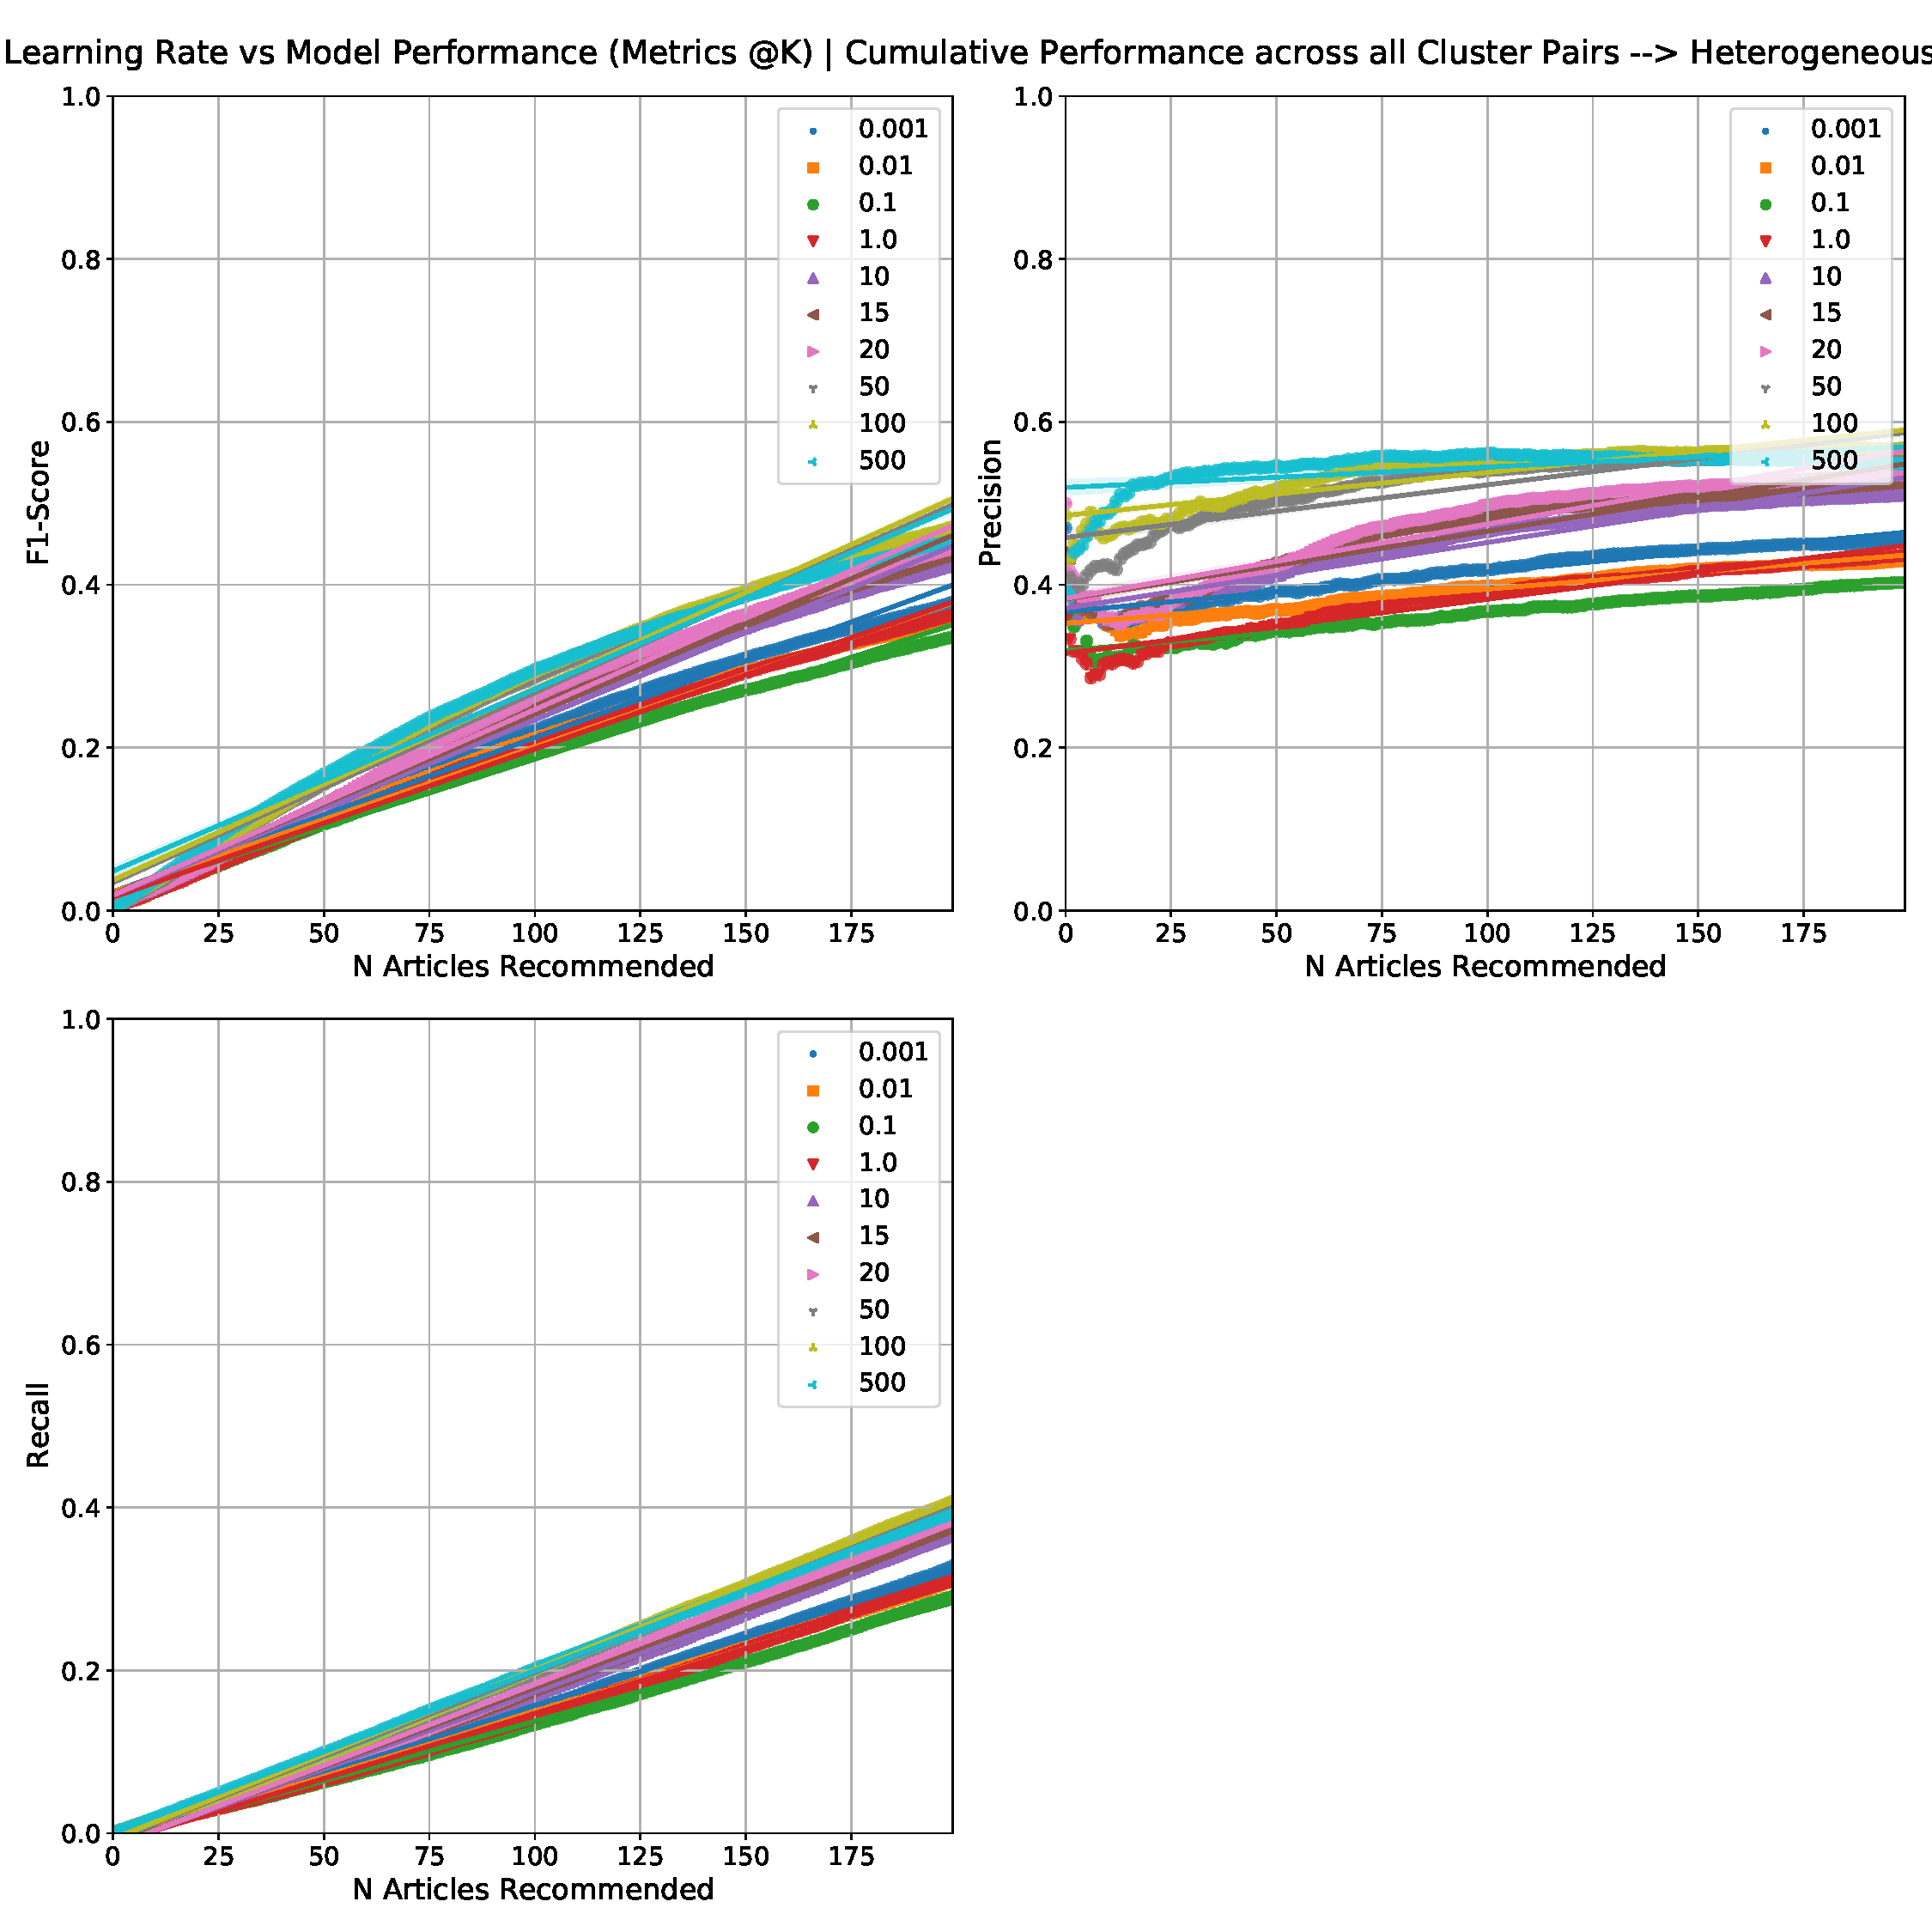
\includegraphics[width=0.6\textwidth]{Graphs/TFIDF/lr_vs_model_performance_cumu_Heterogeneous.pdf}
\end{figure}
\subsection{Glove}
\subsubsection{Homogeneous Users :}
\begin{figure}[H]
 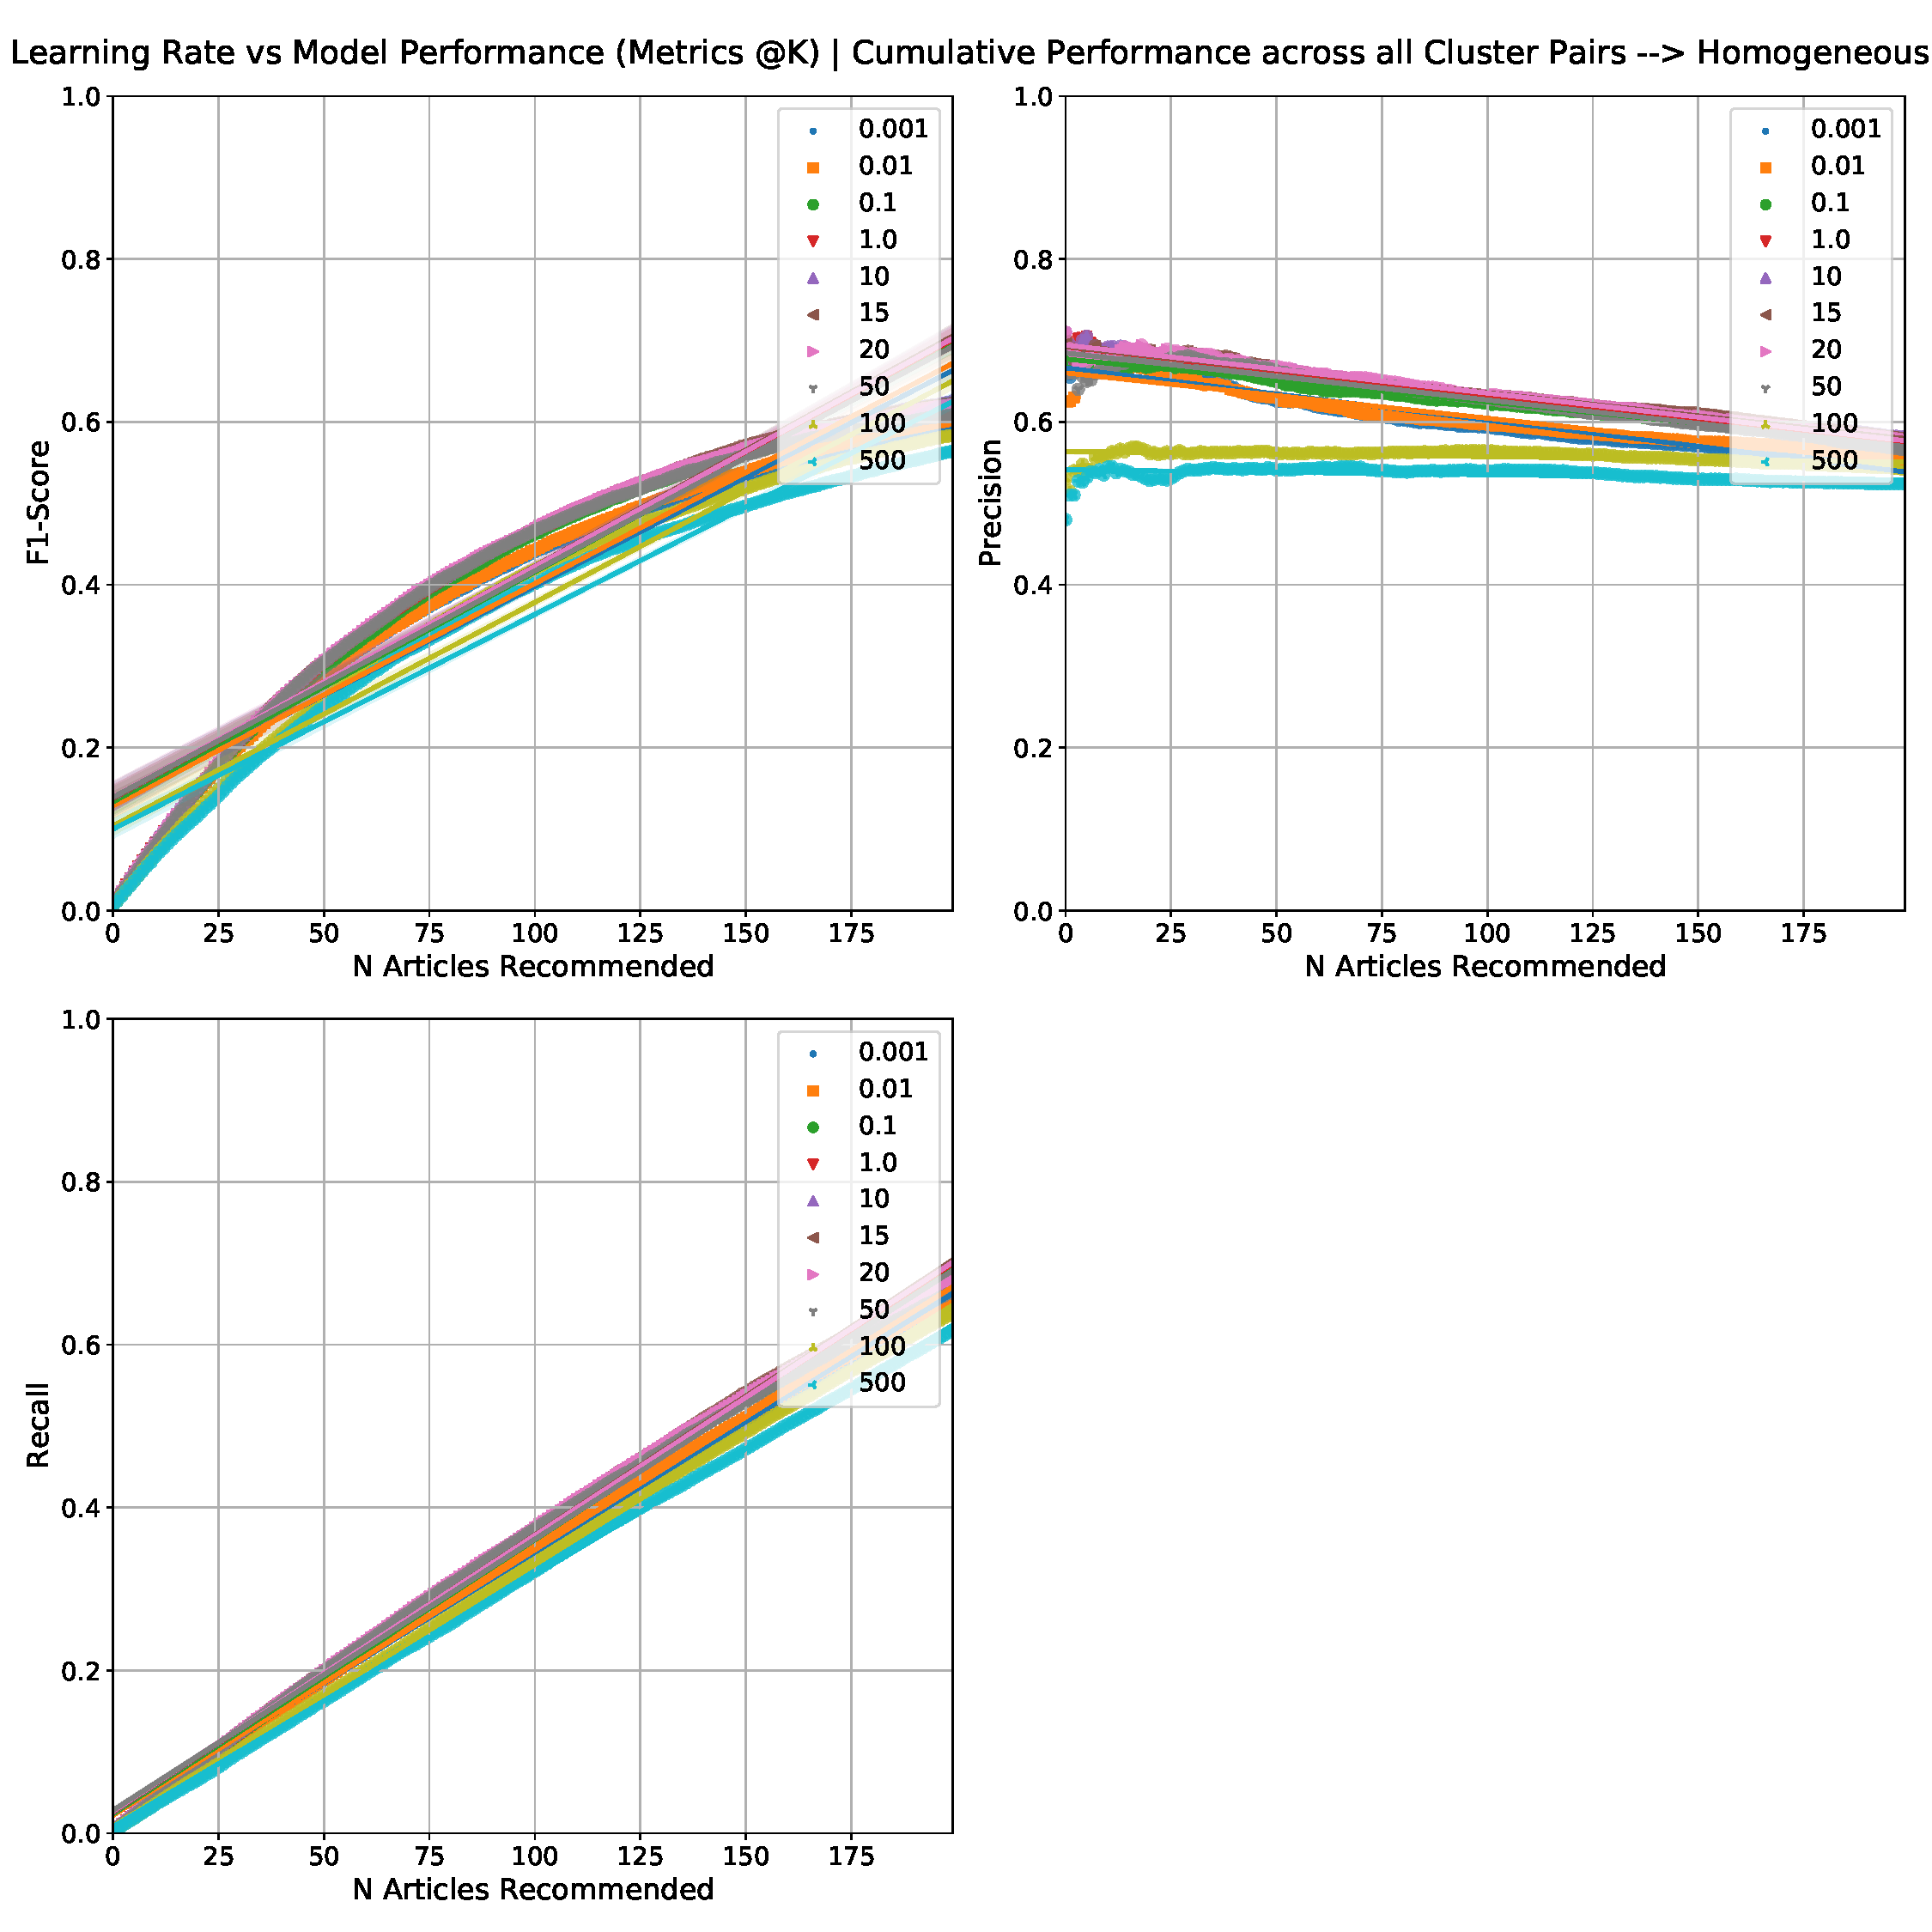
\includegraphics[width=0.6\textwidth]{Graphs/GLOVE/lr_vs_model_performance_cumu_Homogeneous.pdf}
\end{figure}
\subsubsection{Heterogeneous Users :}
\begin{figure}[H]
 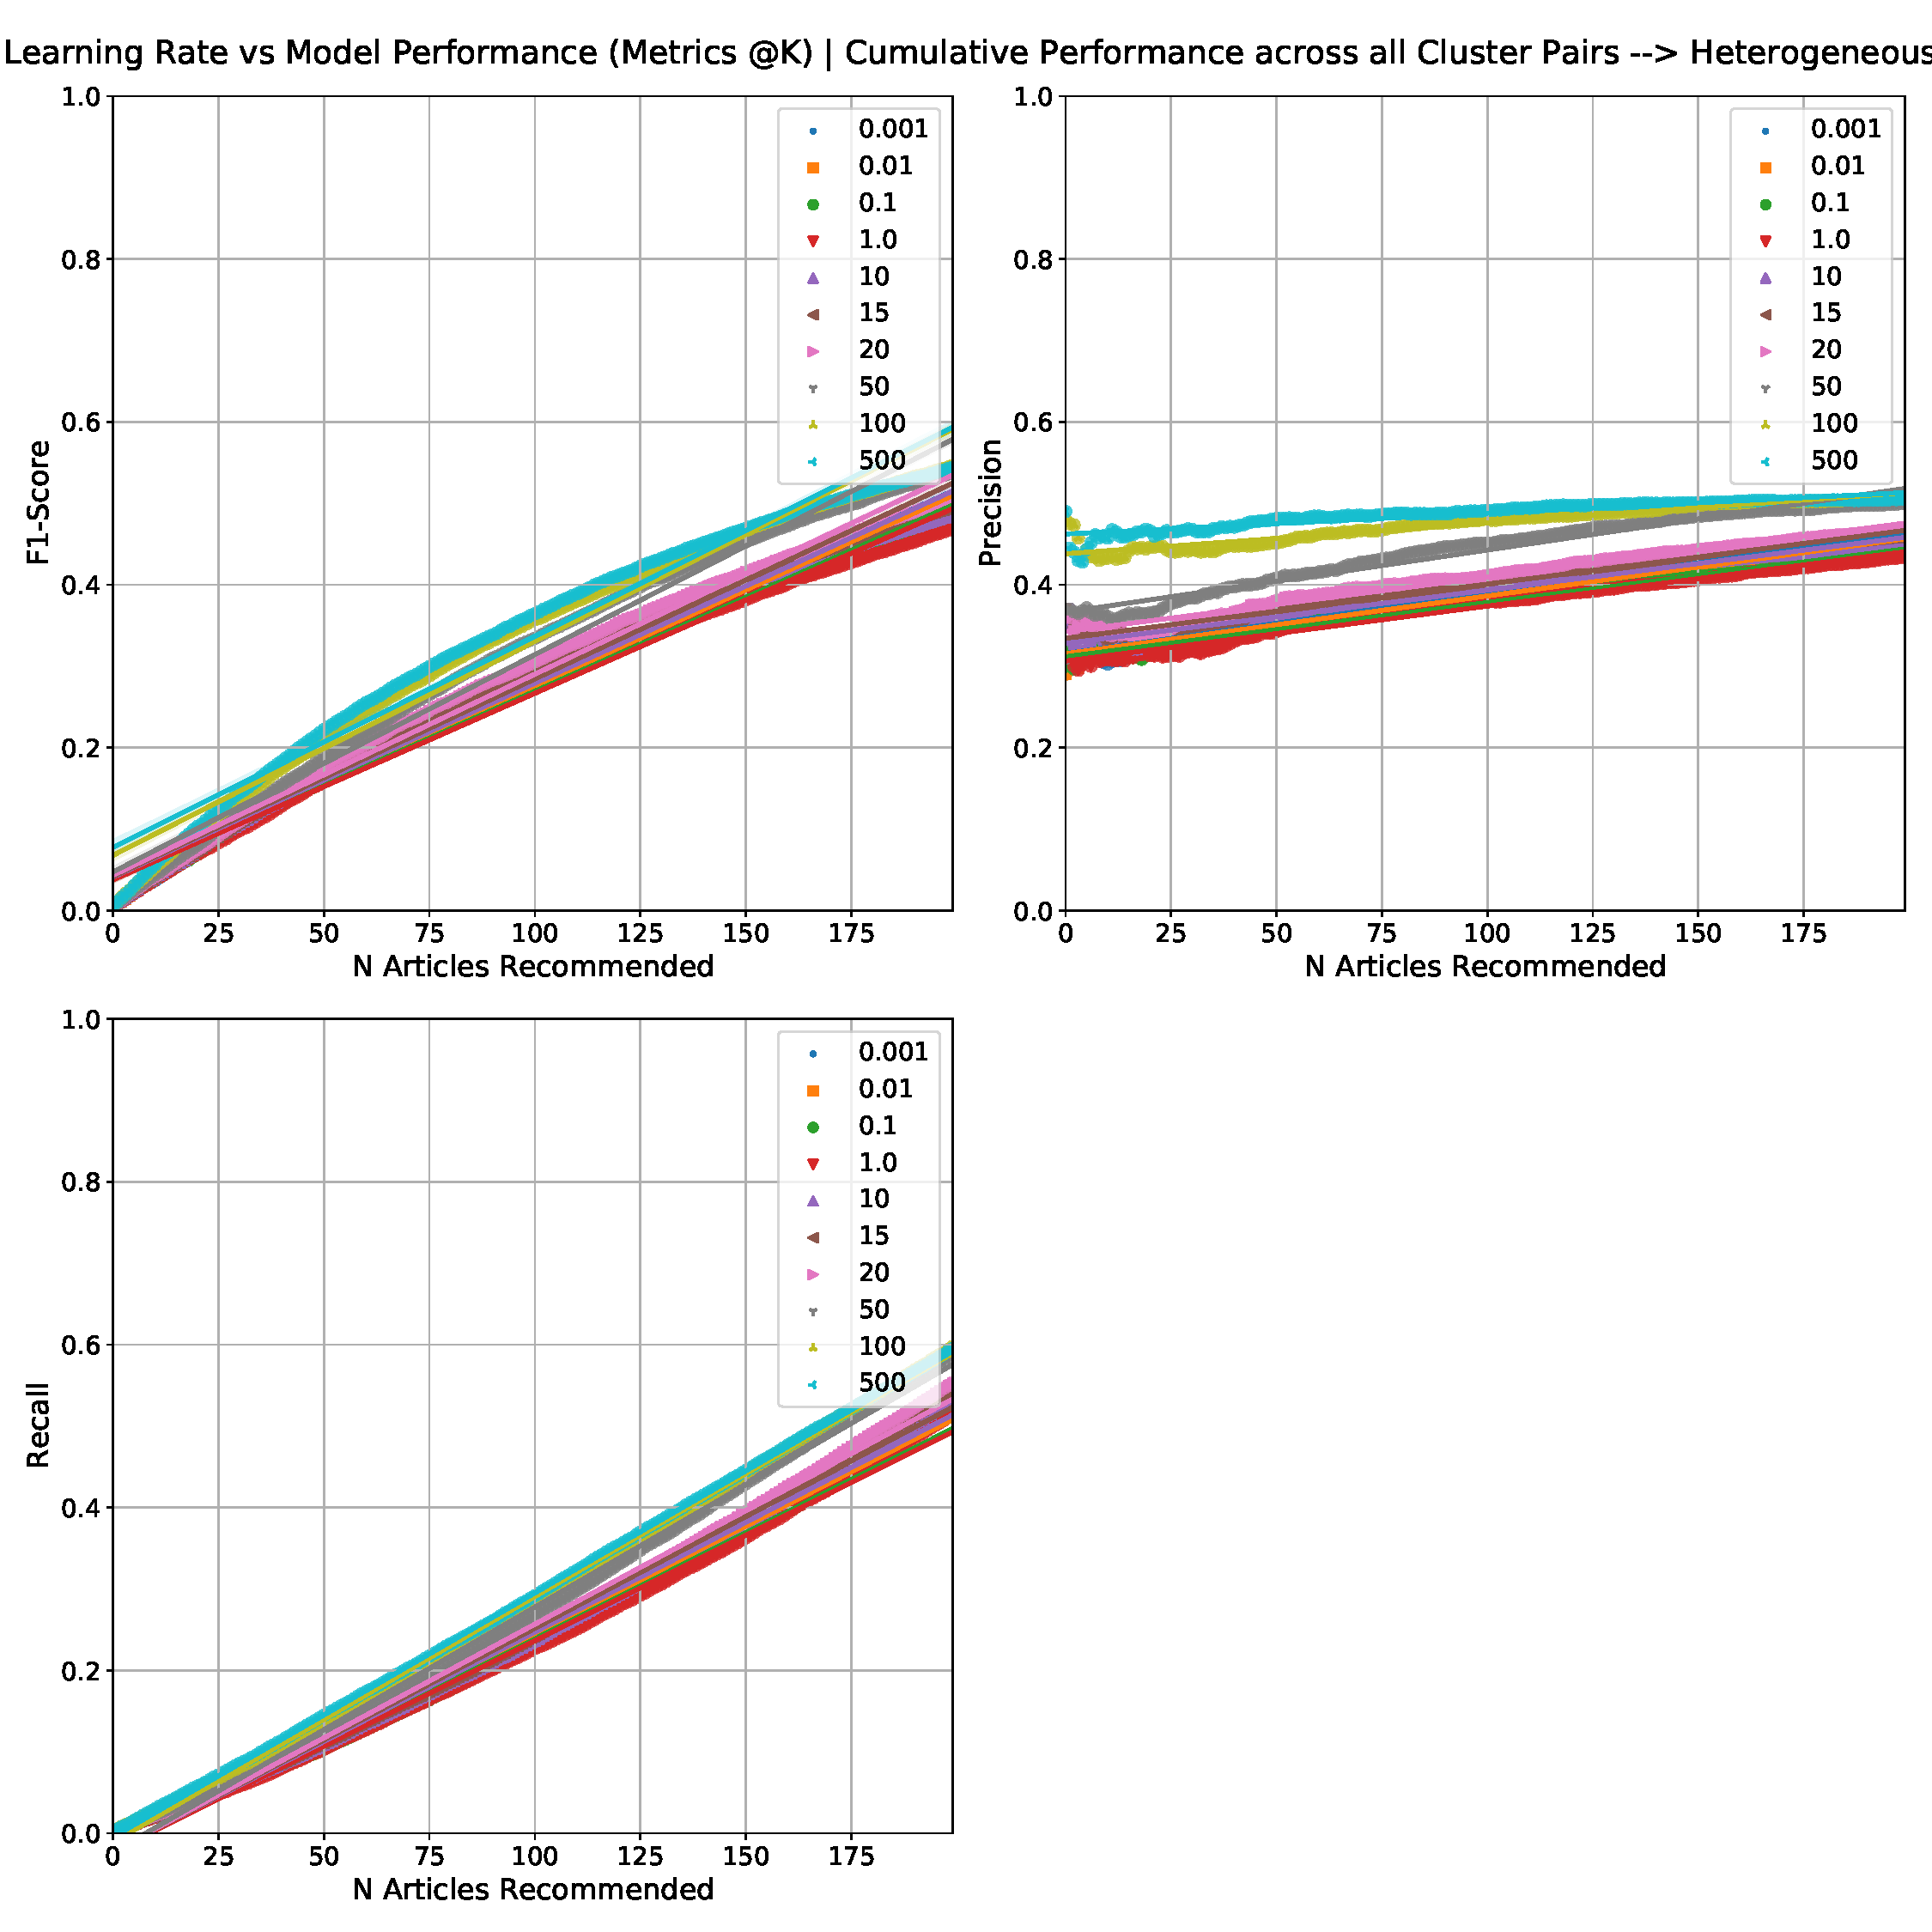
\includegraphics[width=0.6\textwidth]{Graphs/GLOVE/lr_vs_model_performance_cumu_Heterogeneous.pdf}
\end{figure}
\subsection{BERT}
\subsubsection{Homogeneous Users :}
\begin{figure}[H]
 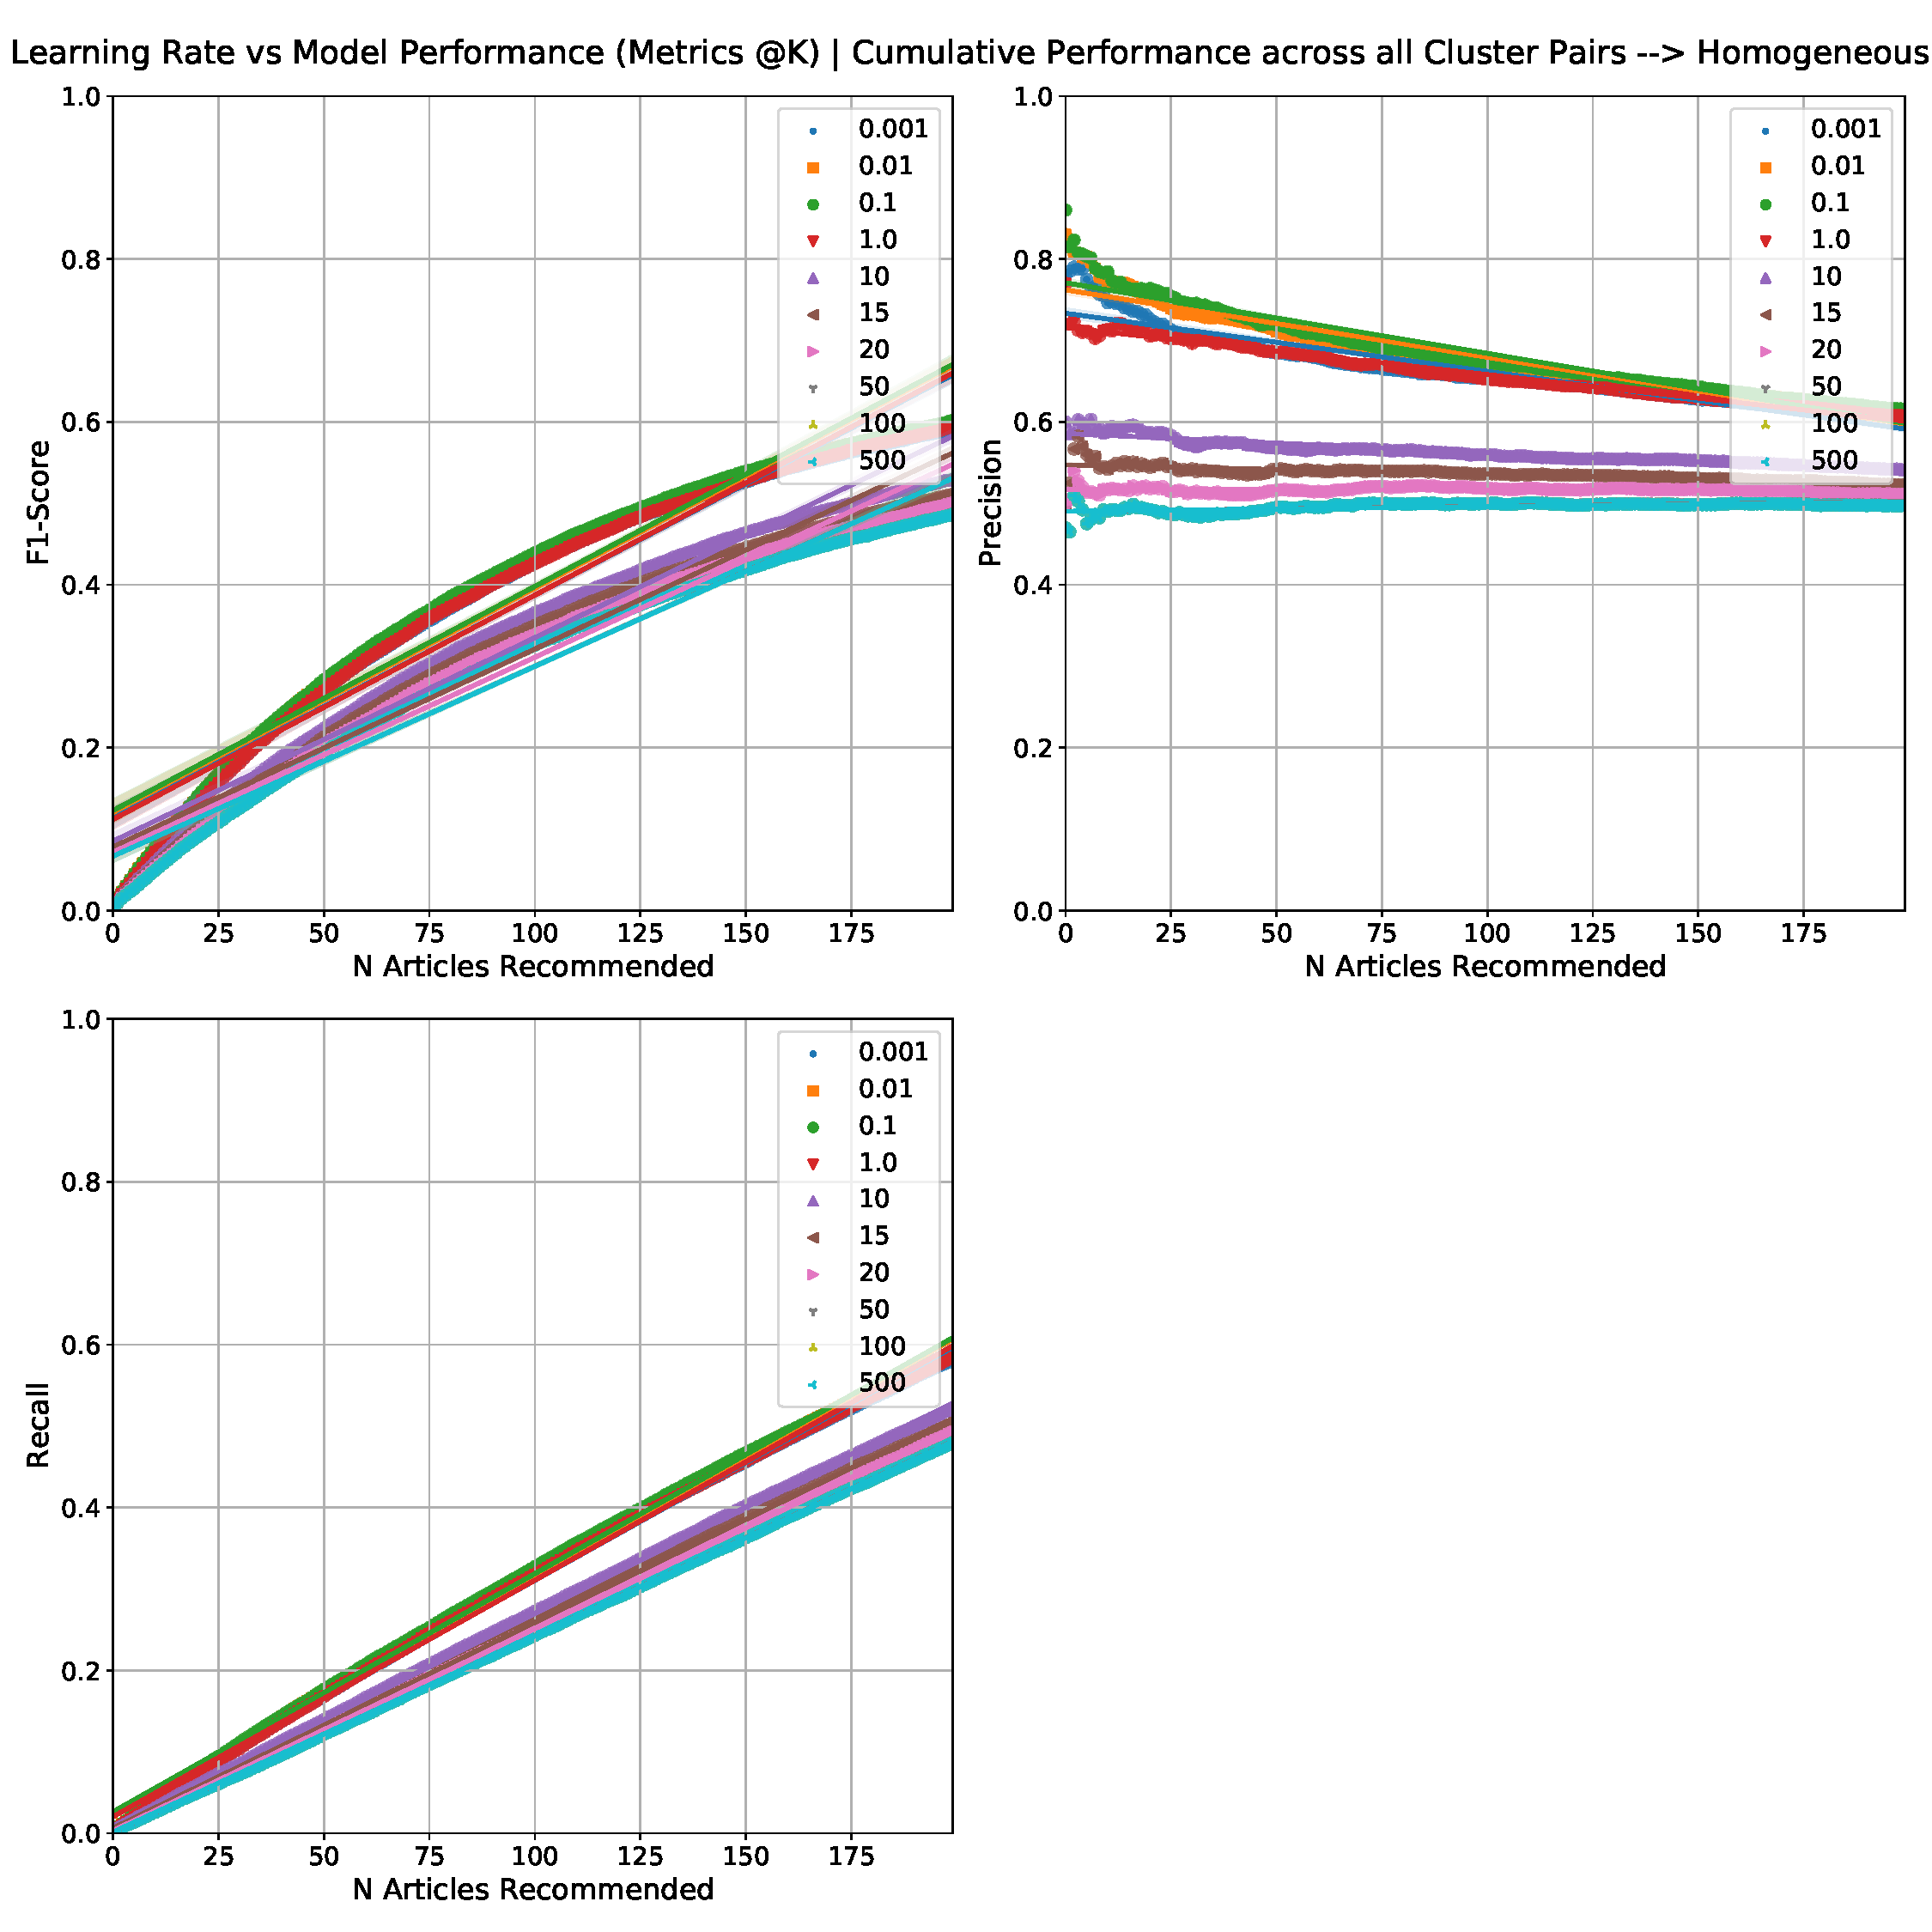
\includegraphics[width=0.6\textwidth]{Graphs/BERT/lr_vs_model_performance_cumu_Homogeneous.pdf}
\end{figure}
\subsubsection{Heterogeneous Users :}
\begin{figure}[H]
 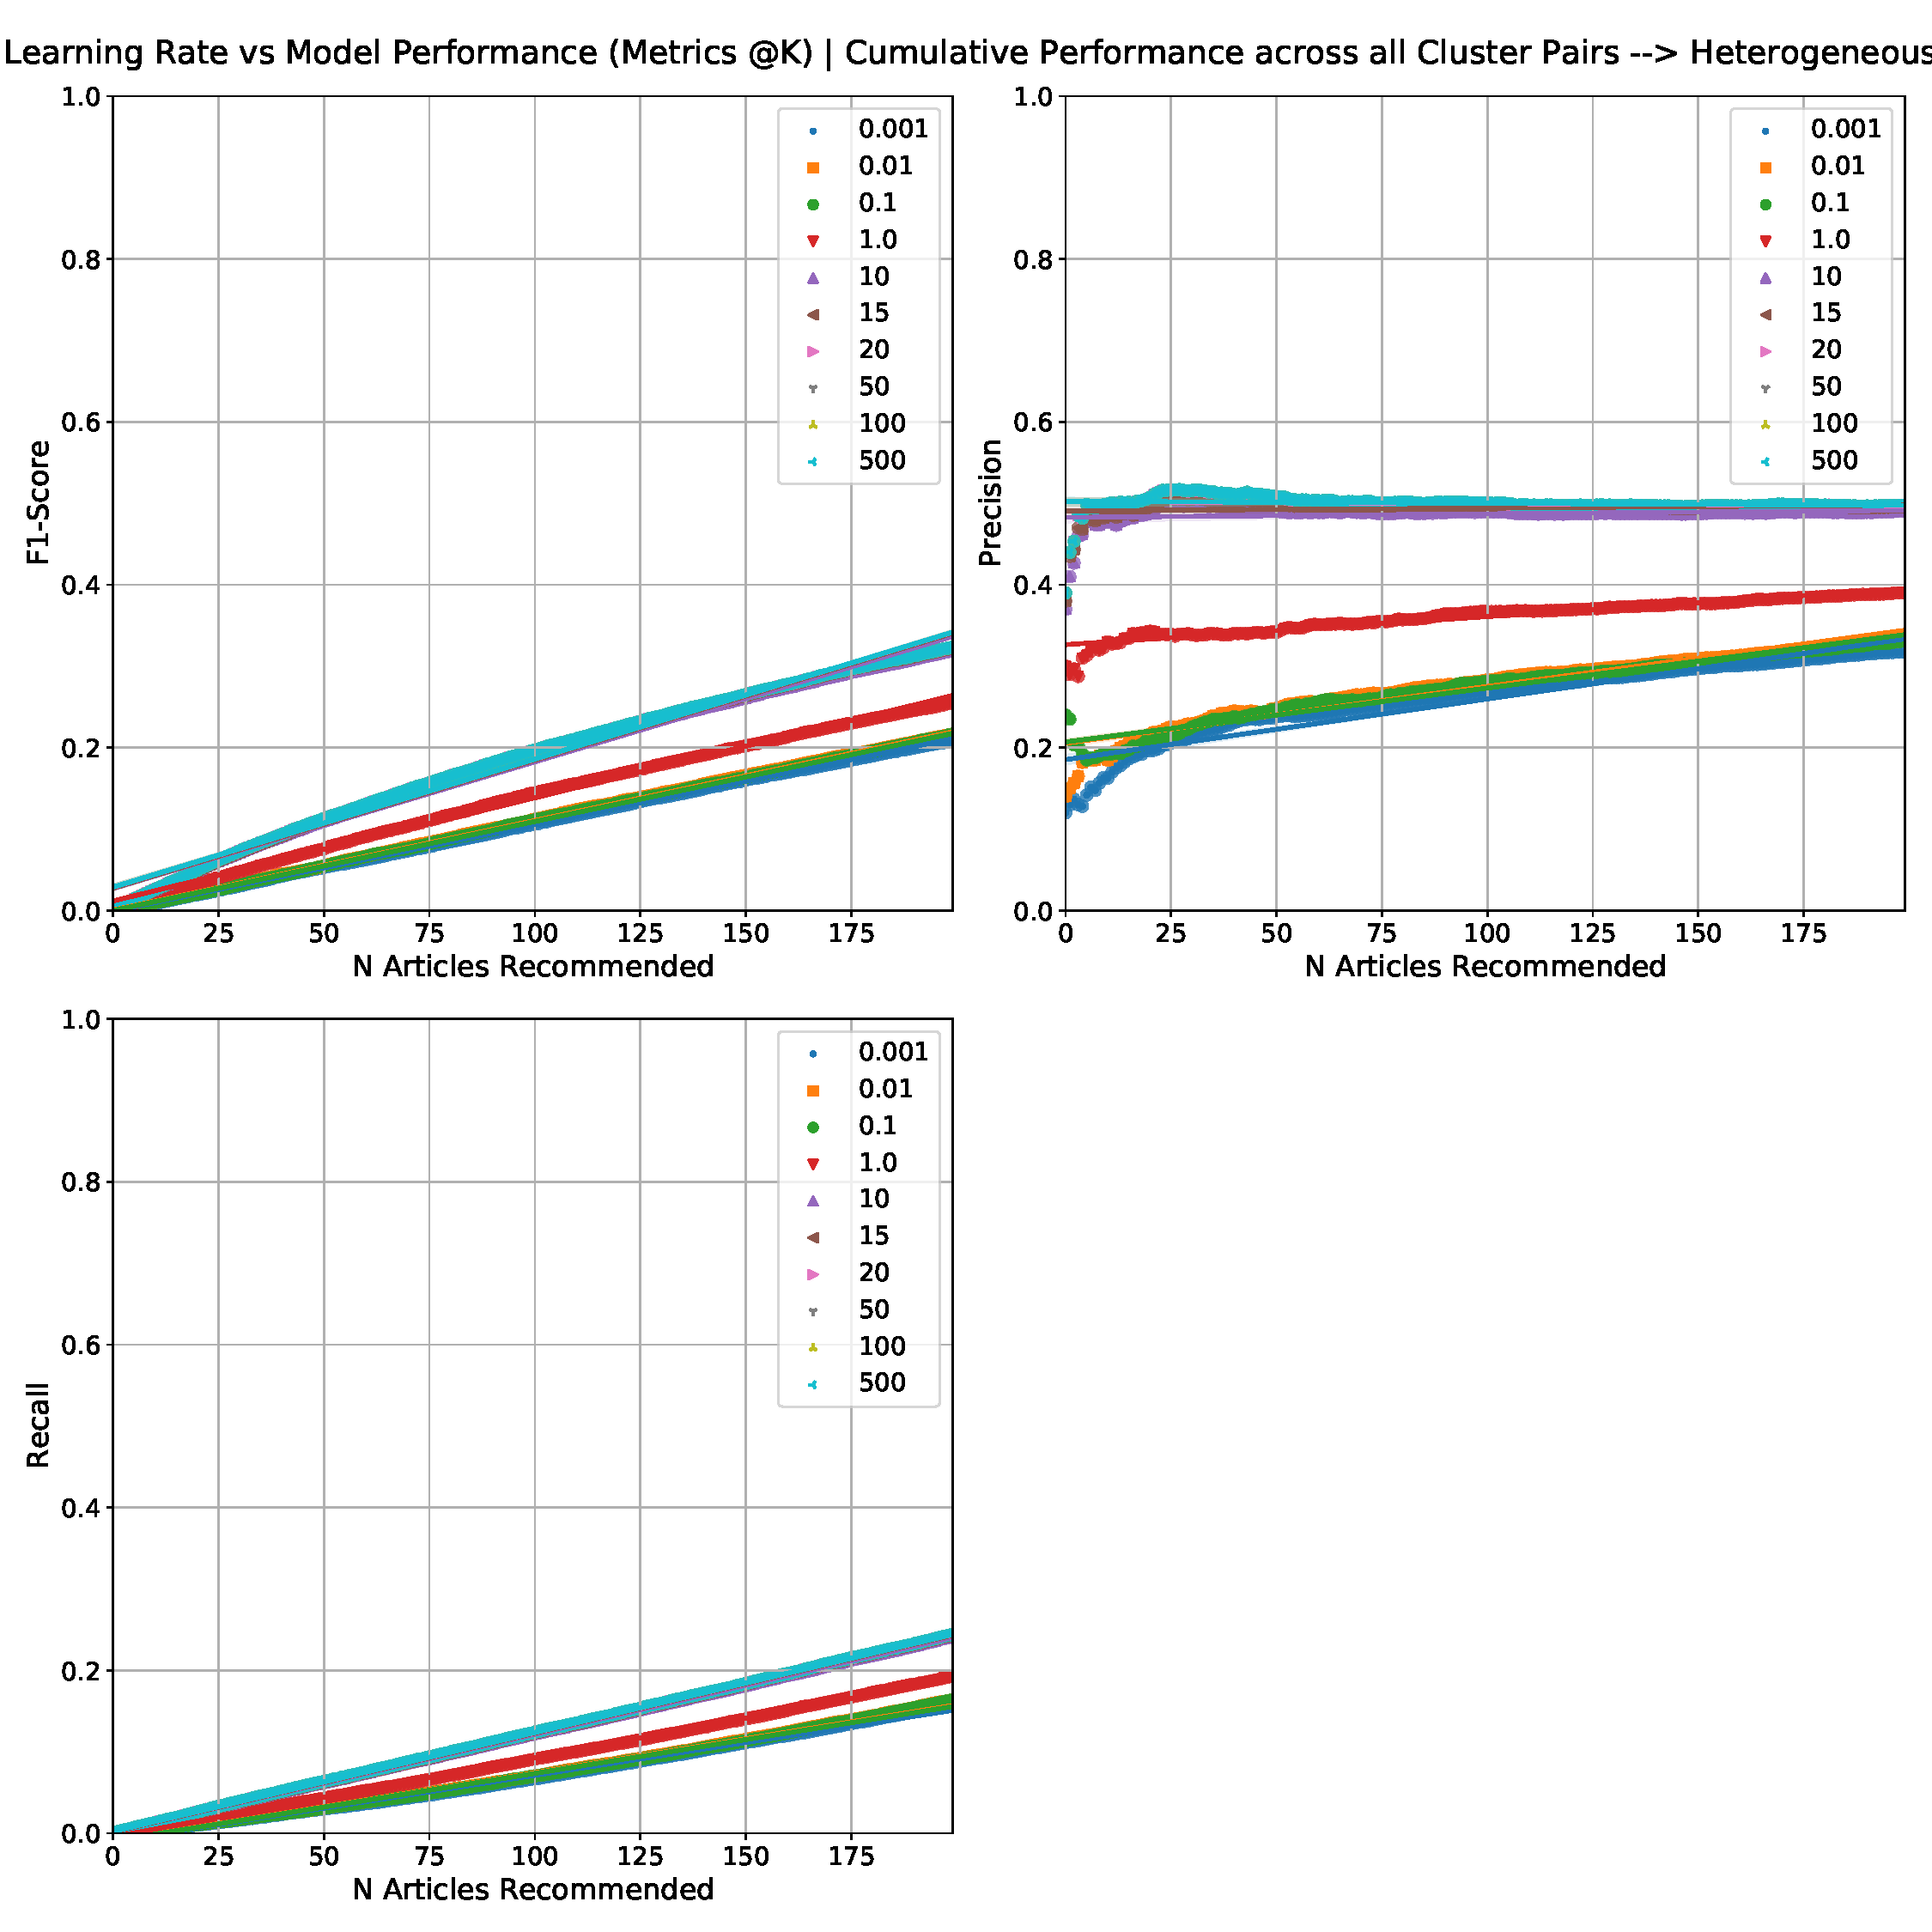
\includegraphics[width=0.6\textwidth]{Graphs/BERT/lr_vs_model_performance_cumu_Heterogeneous.pdf}
\end{figure}

\newpage
\section{Baseline 6: Model Performance on mixed Set (Cluster 1 + Cluster 2)}
\begin{flushleft}
We want to measure how well the model would perform when an article from an unseen topic arrives along with articles from the original topic the classifier was trained on
\end{flushleft}
\subsection{TF-IDF}
\begin{figure}[H]
    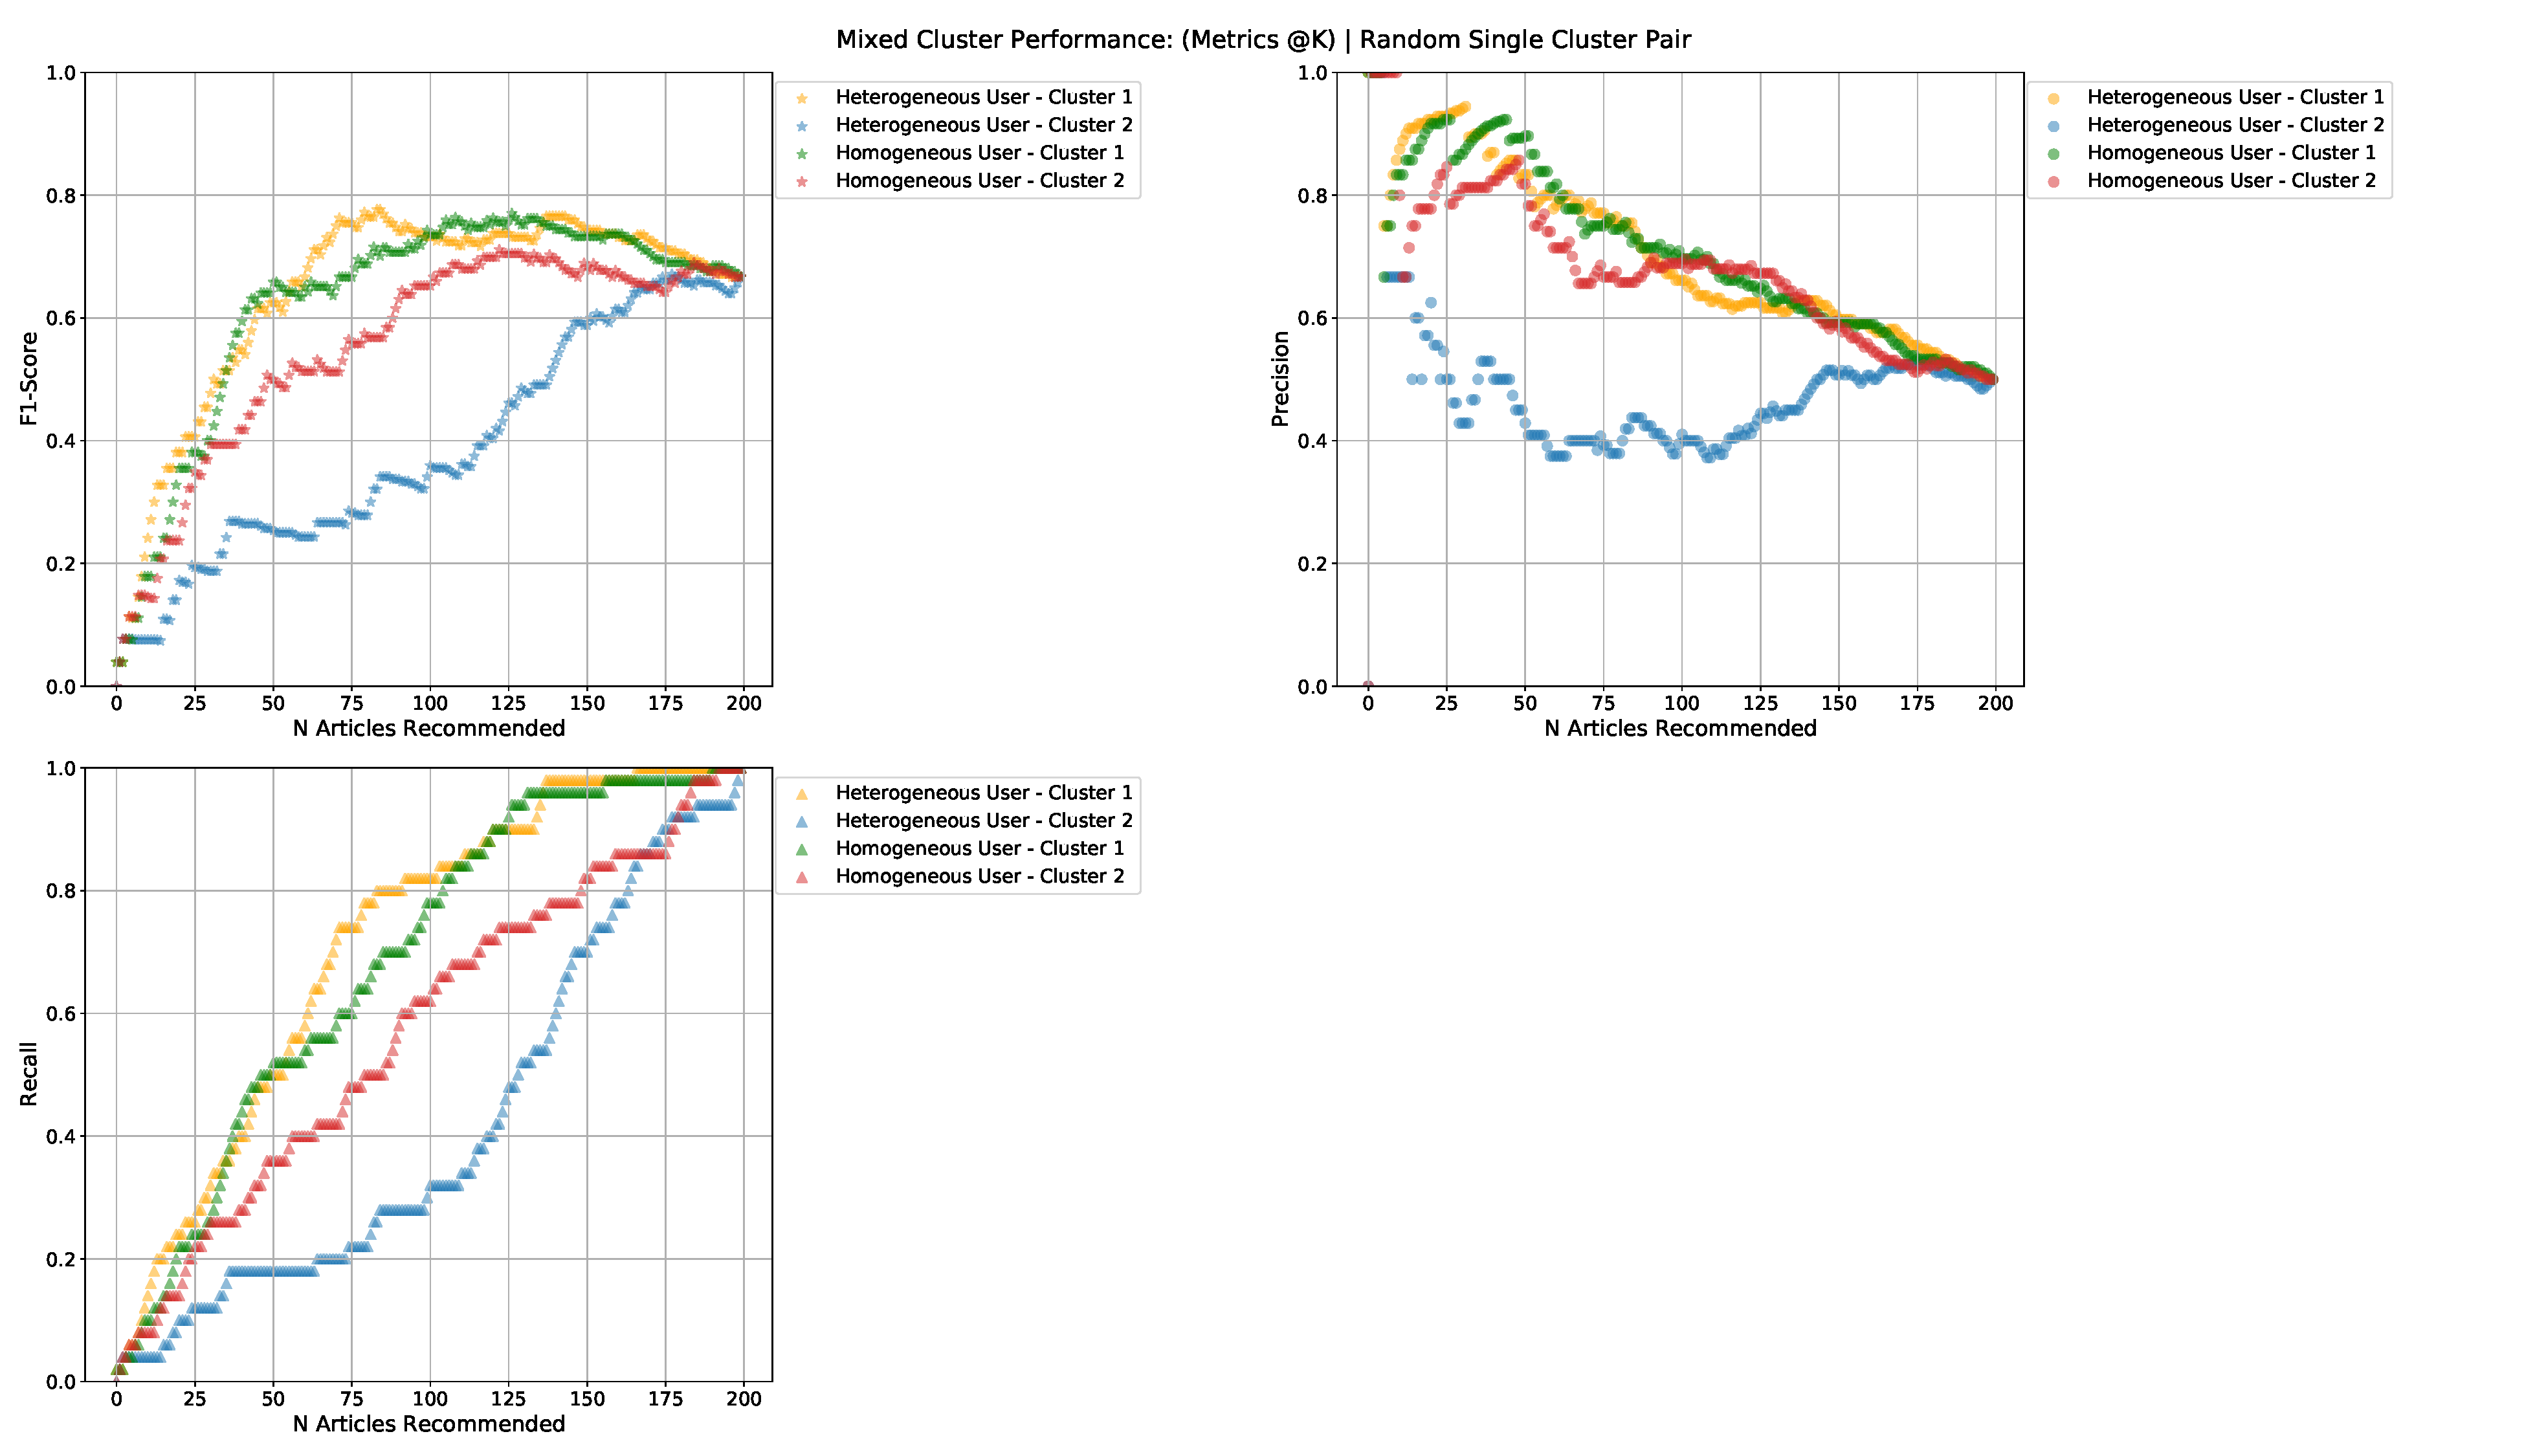
\includegraphics[width=1.0\textwidth]{Graphs/TFIDF/user_interaction_vs_model_performance_mixed_cluster.pdf}
    % \caption{Caption}
    % \label{fig:my_label}
\end{figure}
\begin{figure}[H]
 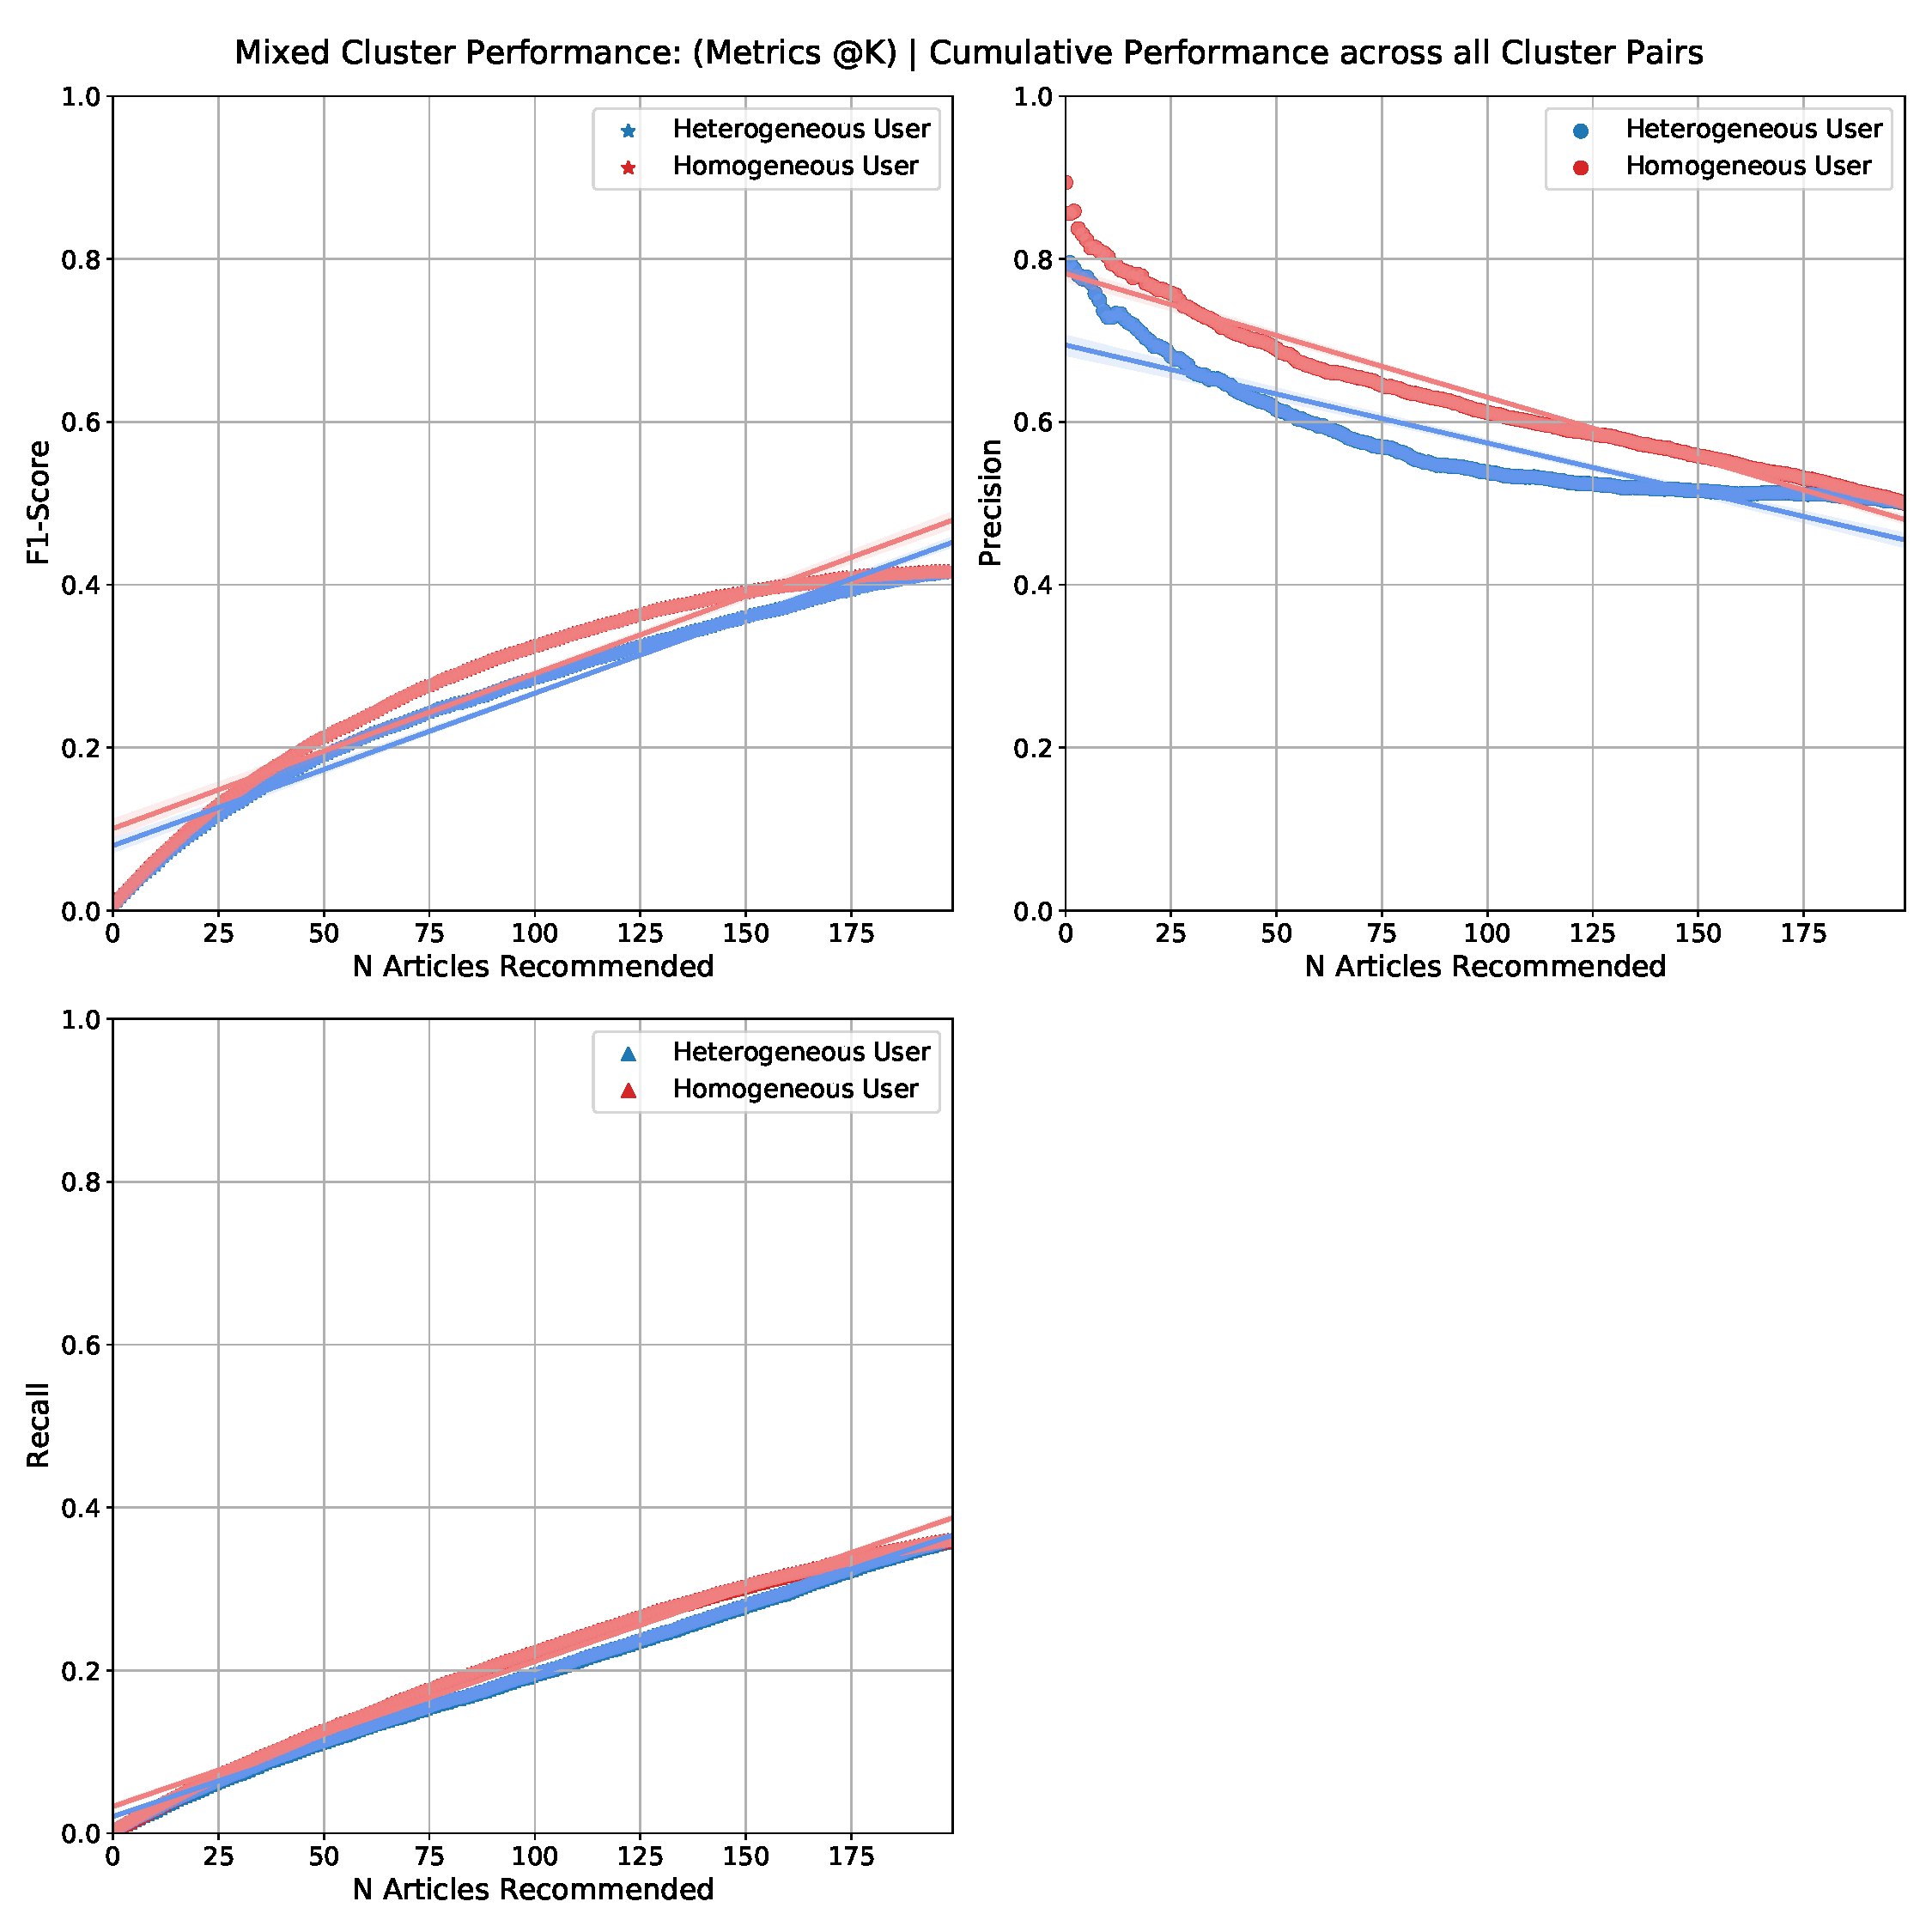
\includegraphics[width=0.6\textwidth]{Graphs/TFIDF/user_interaction_vs_model_performance_cumu_mixed_cluster.pdf}
\end{figure}
\begin{figure}[H]
 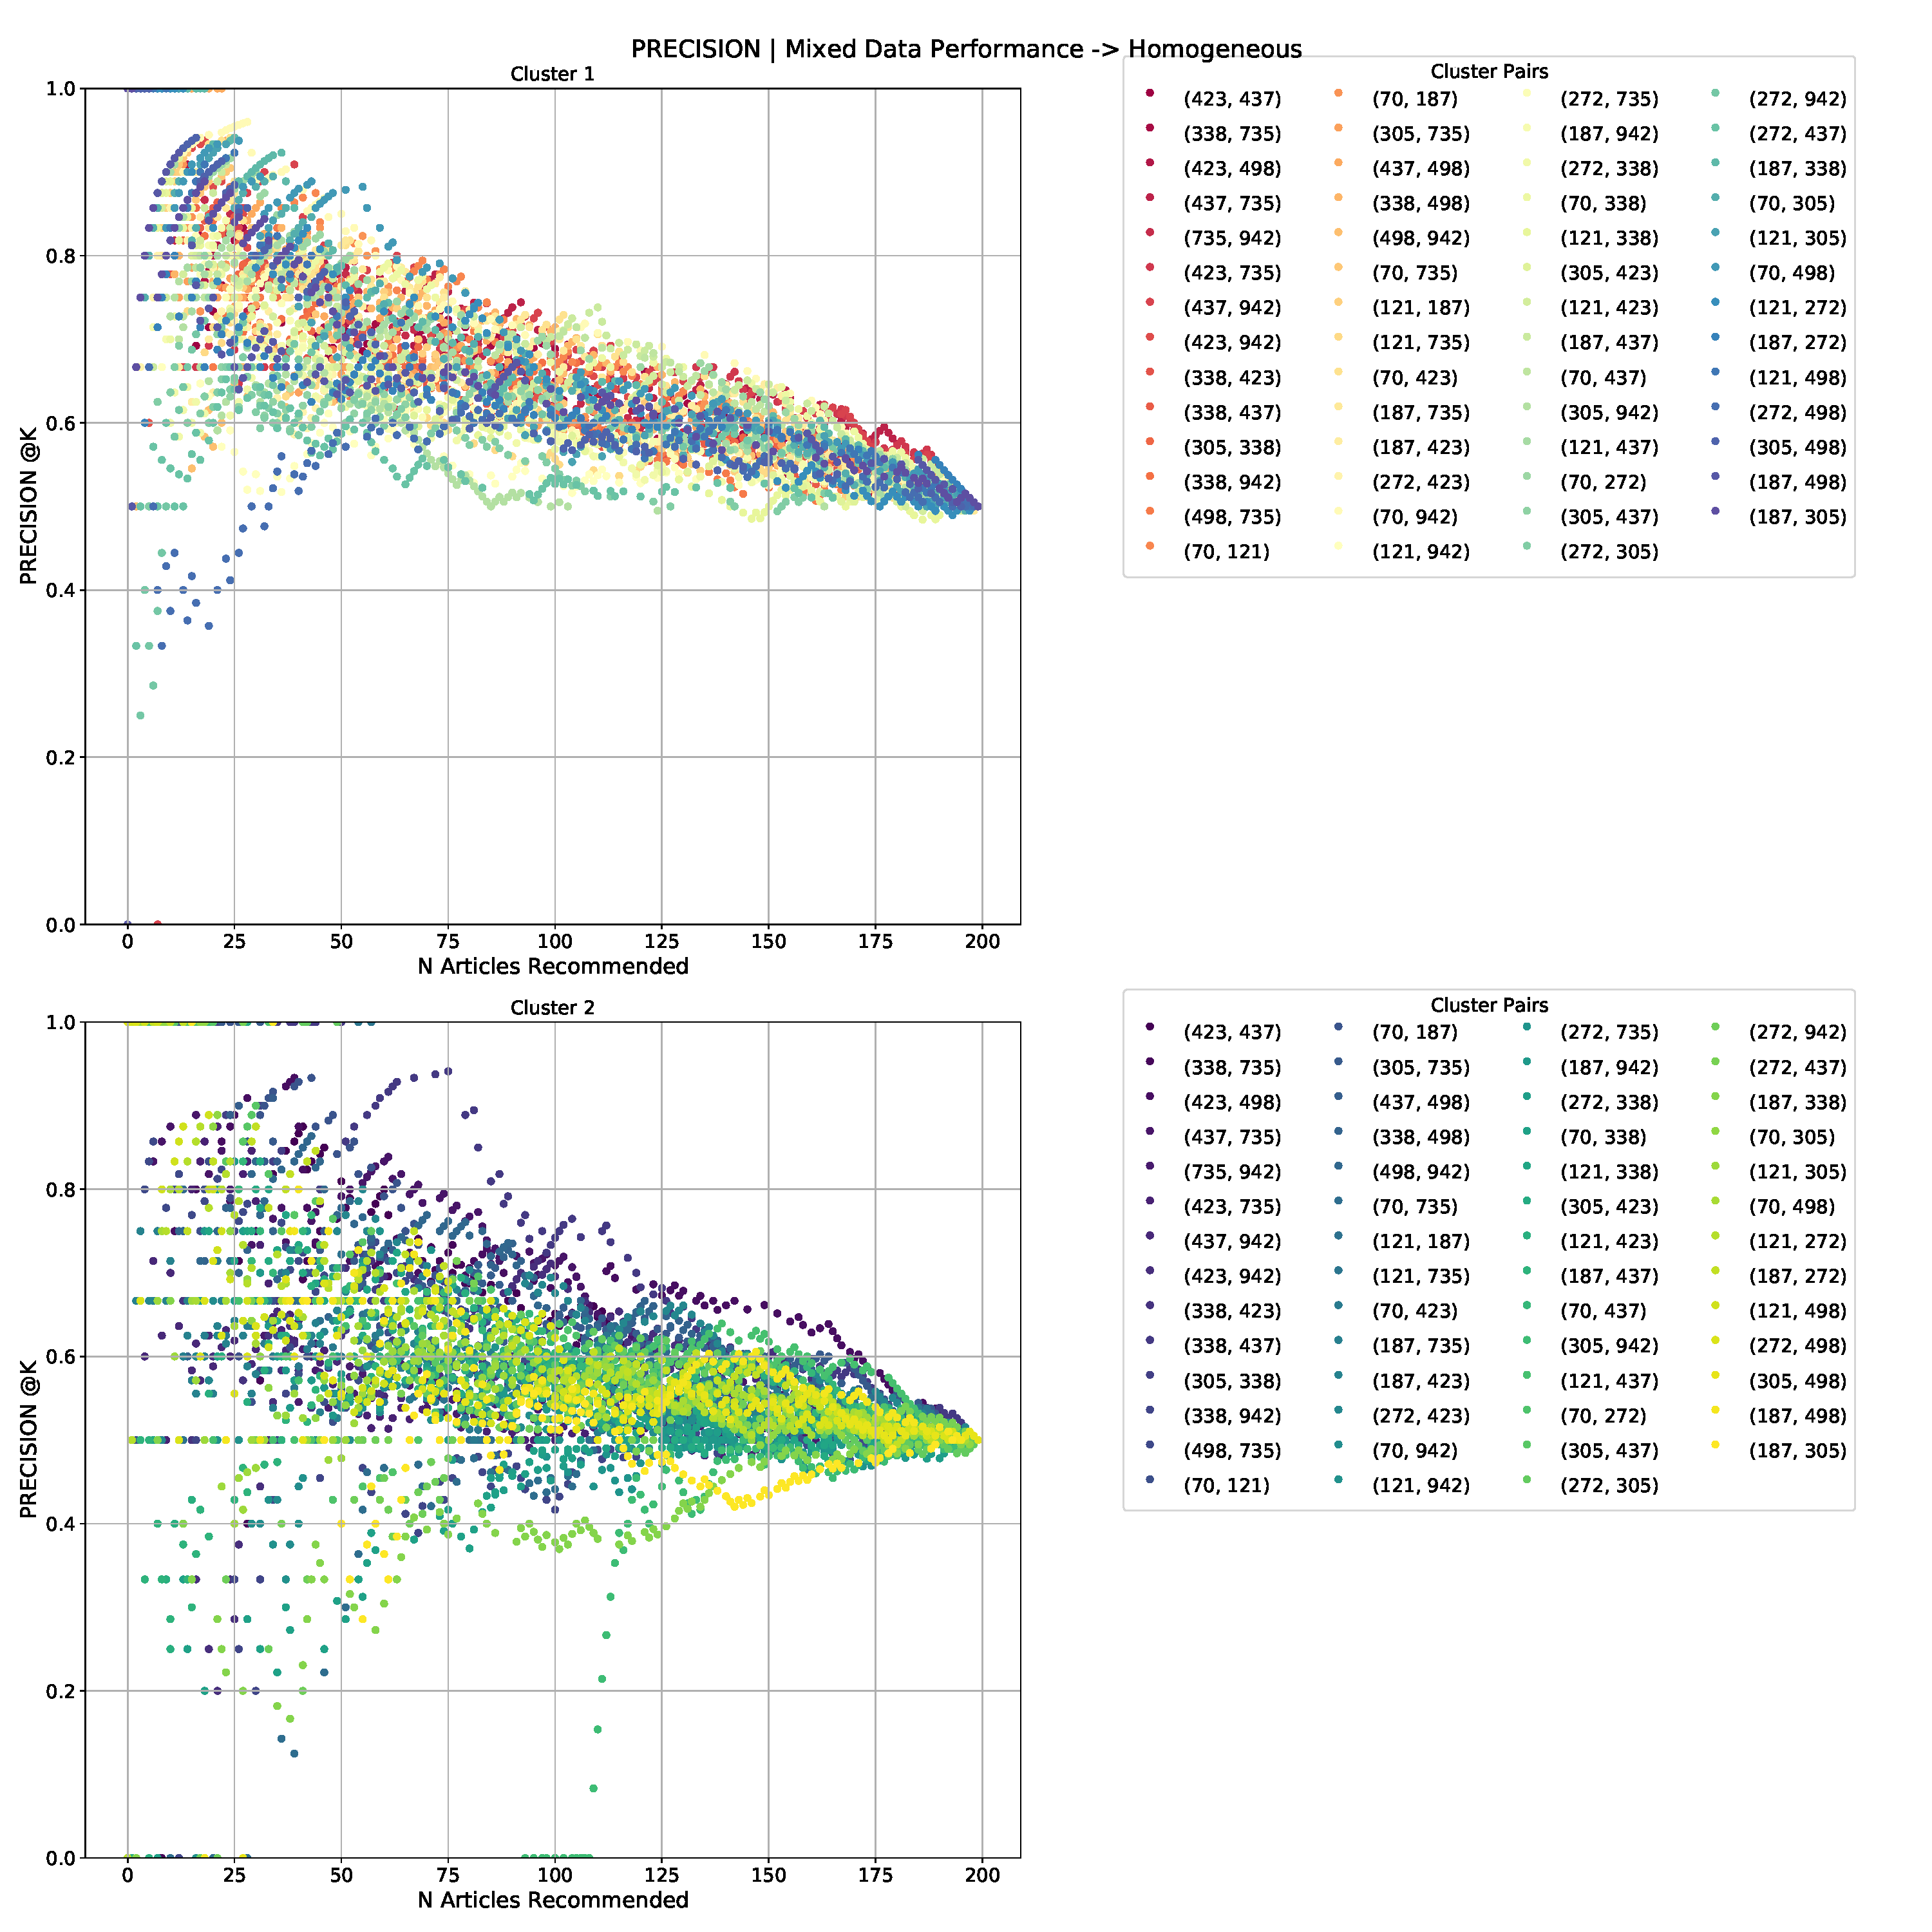
\includegraphics[width=0.7\textwidth]{Graphs/TFIDF/user_interaction_vs_model_performance_precision_all_cps_mixed_data_sep_Homogeneous.pdf}
\end{figure}
\begin{figure}[H]
 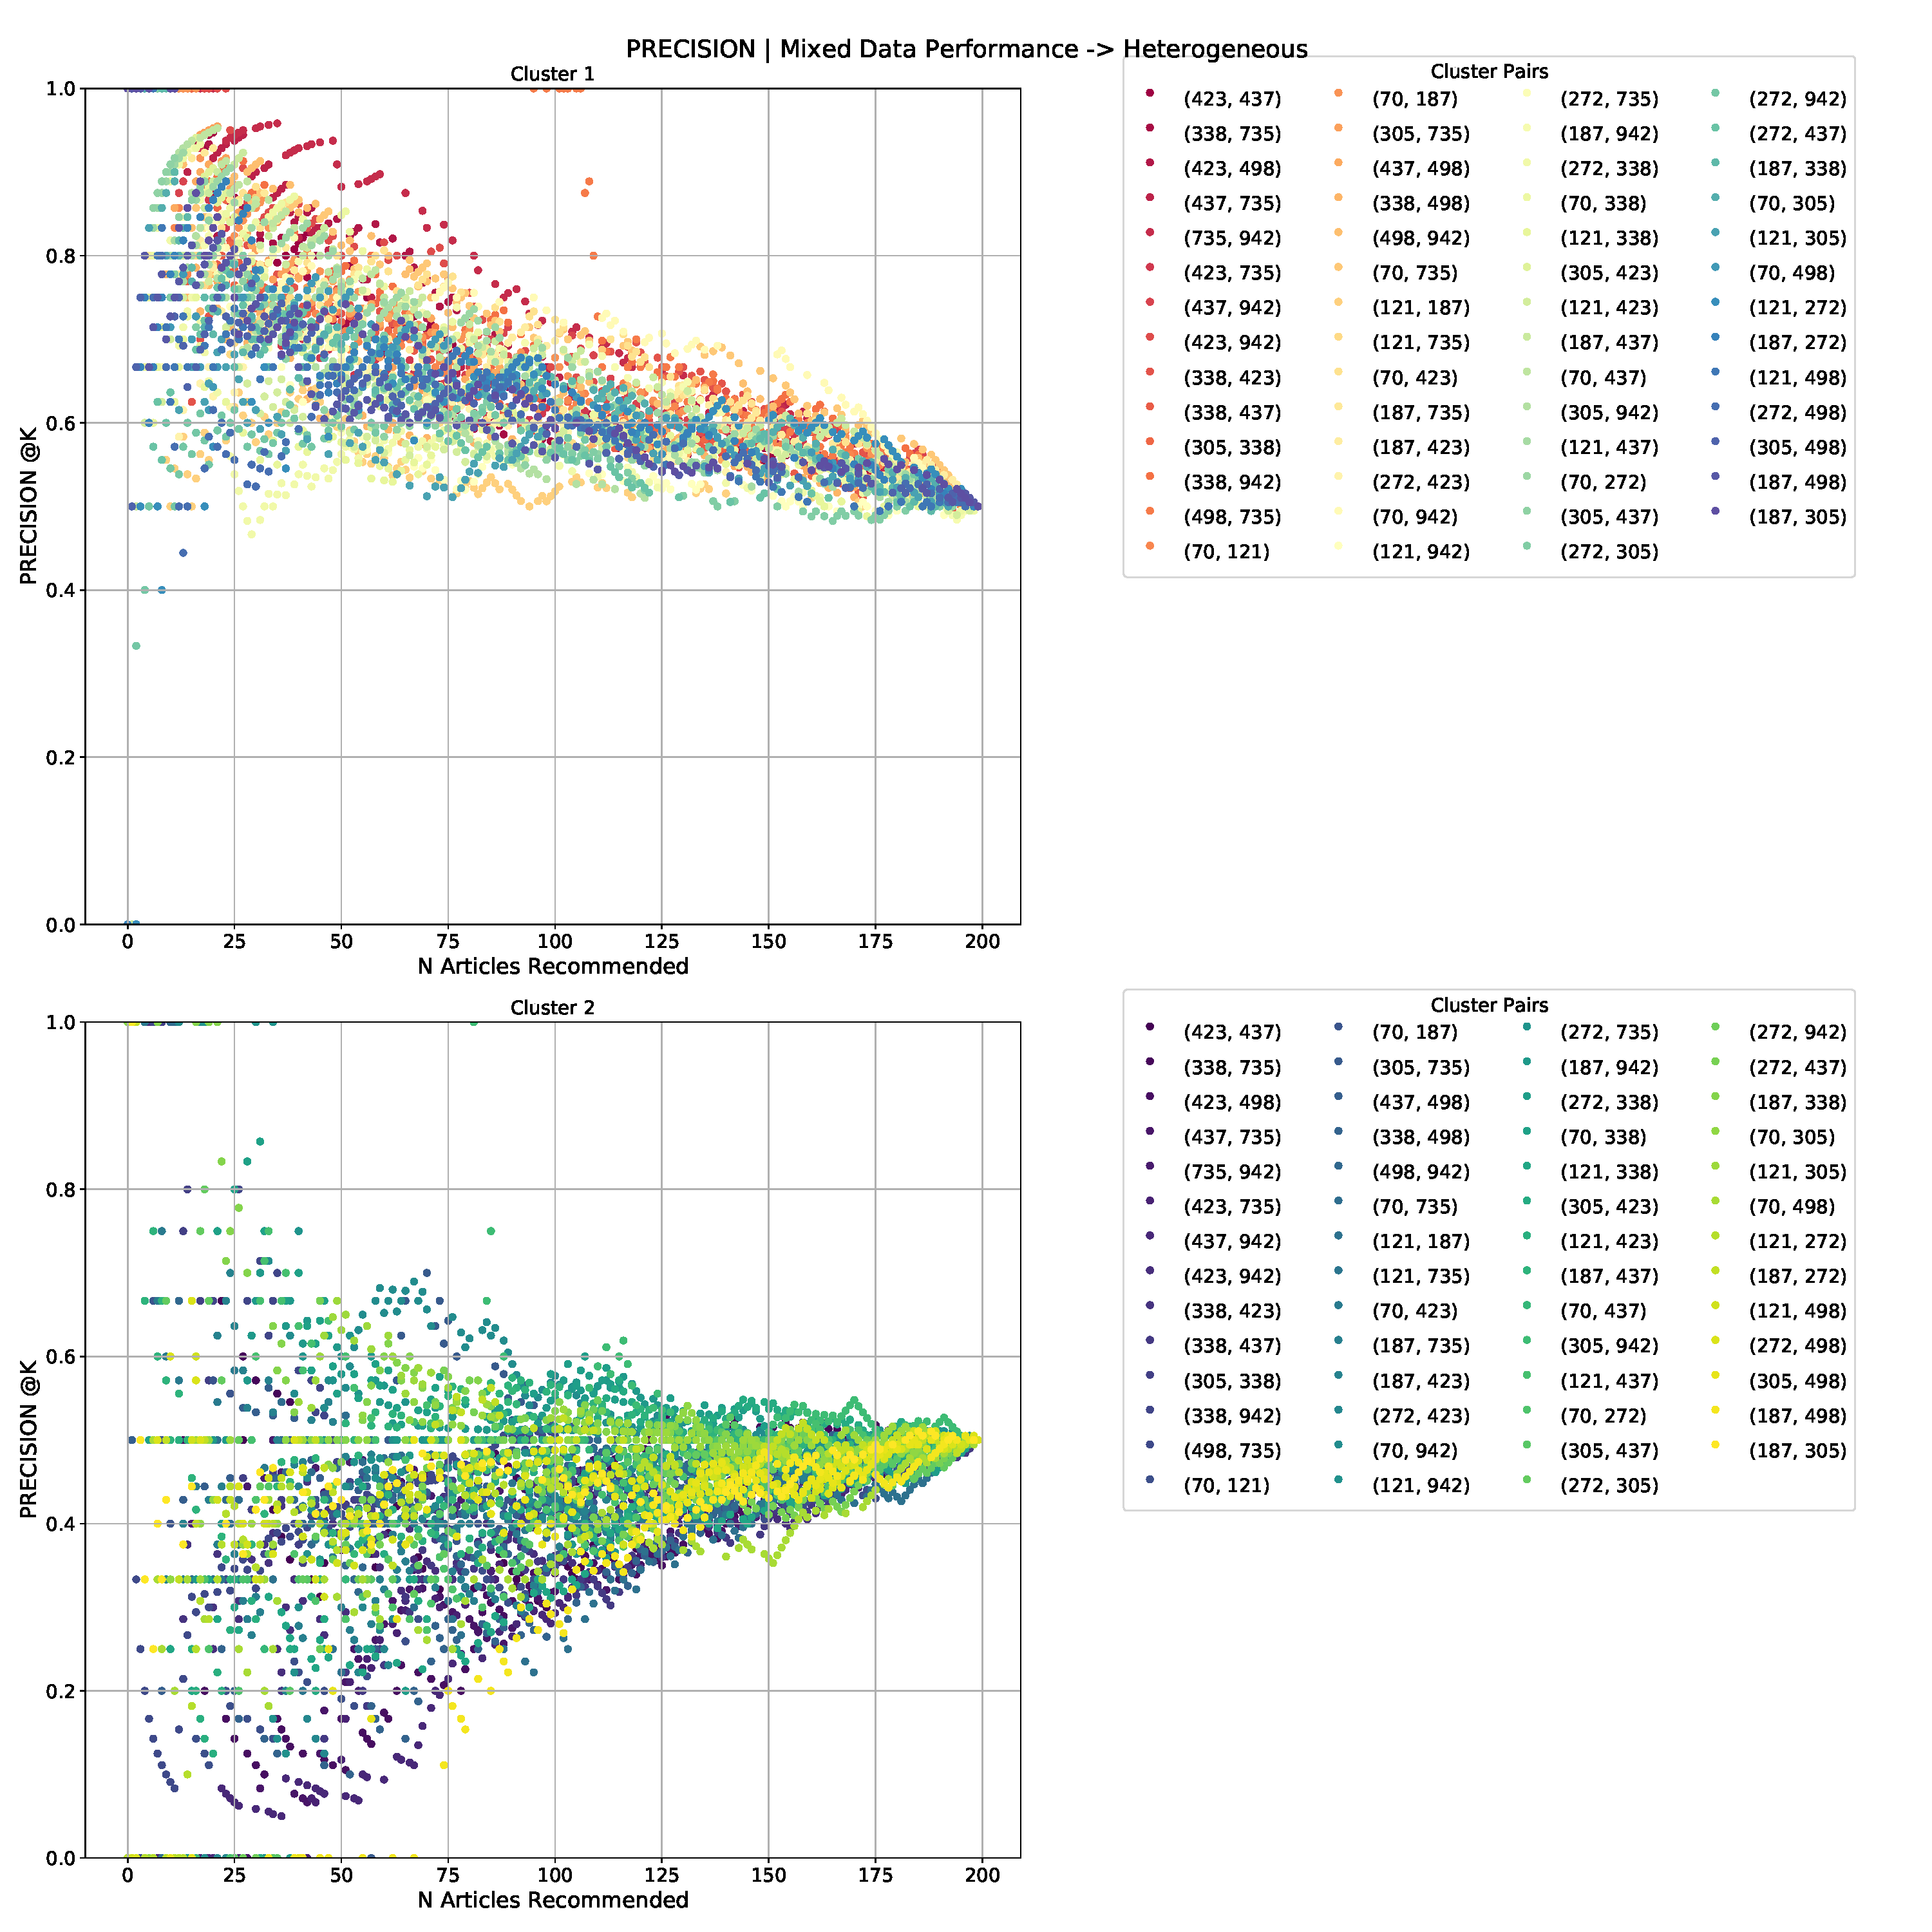
\includegraphics[width=0.7\textwidth]{Graphs/TFIDF/user_interaction_vs_model_performance_precision_all_cps_mixed_data_sep_Heterogeneous.pdf}
\end{figure}
\subsection{Glove}
\begin{figure}[H]
    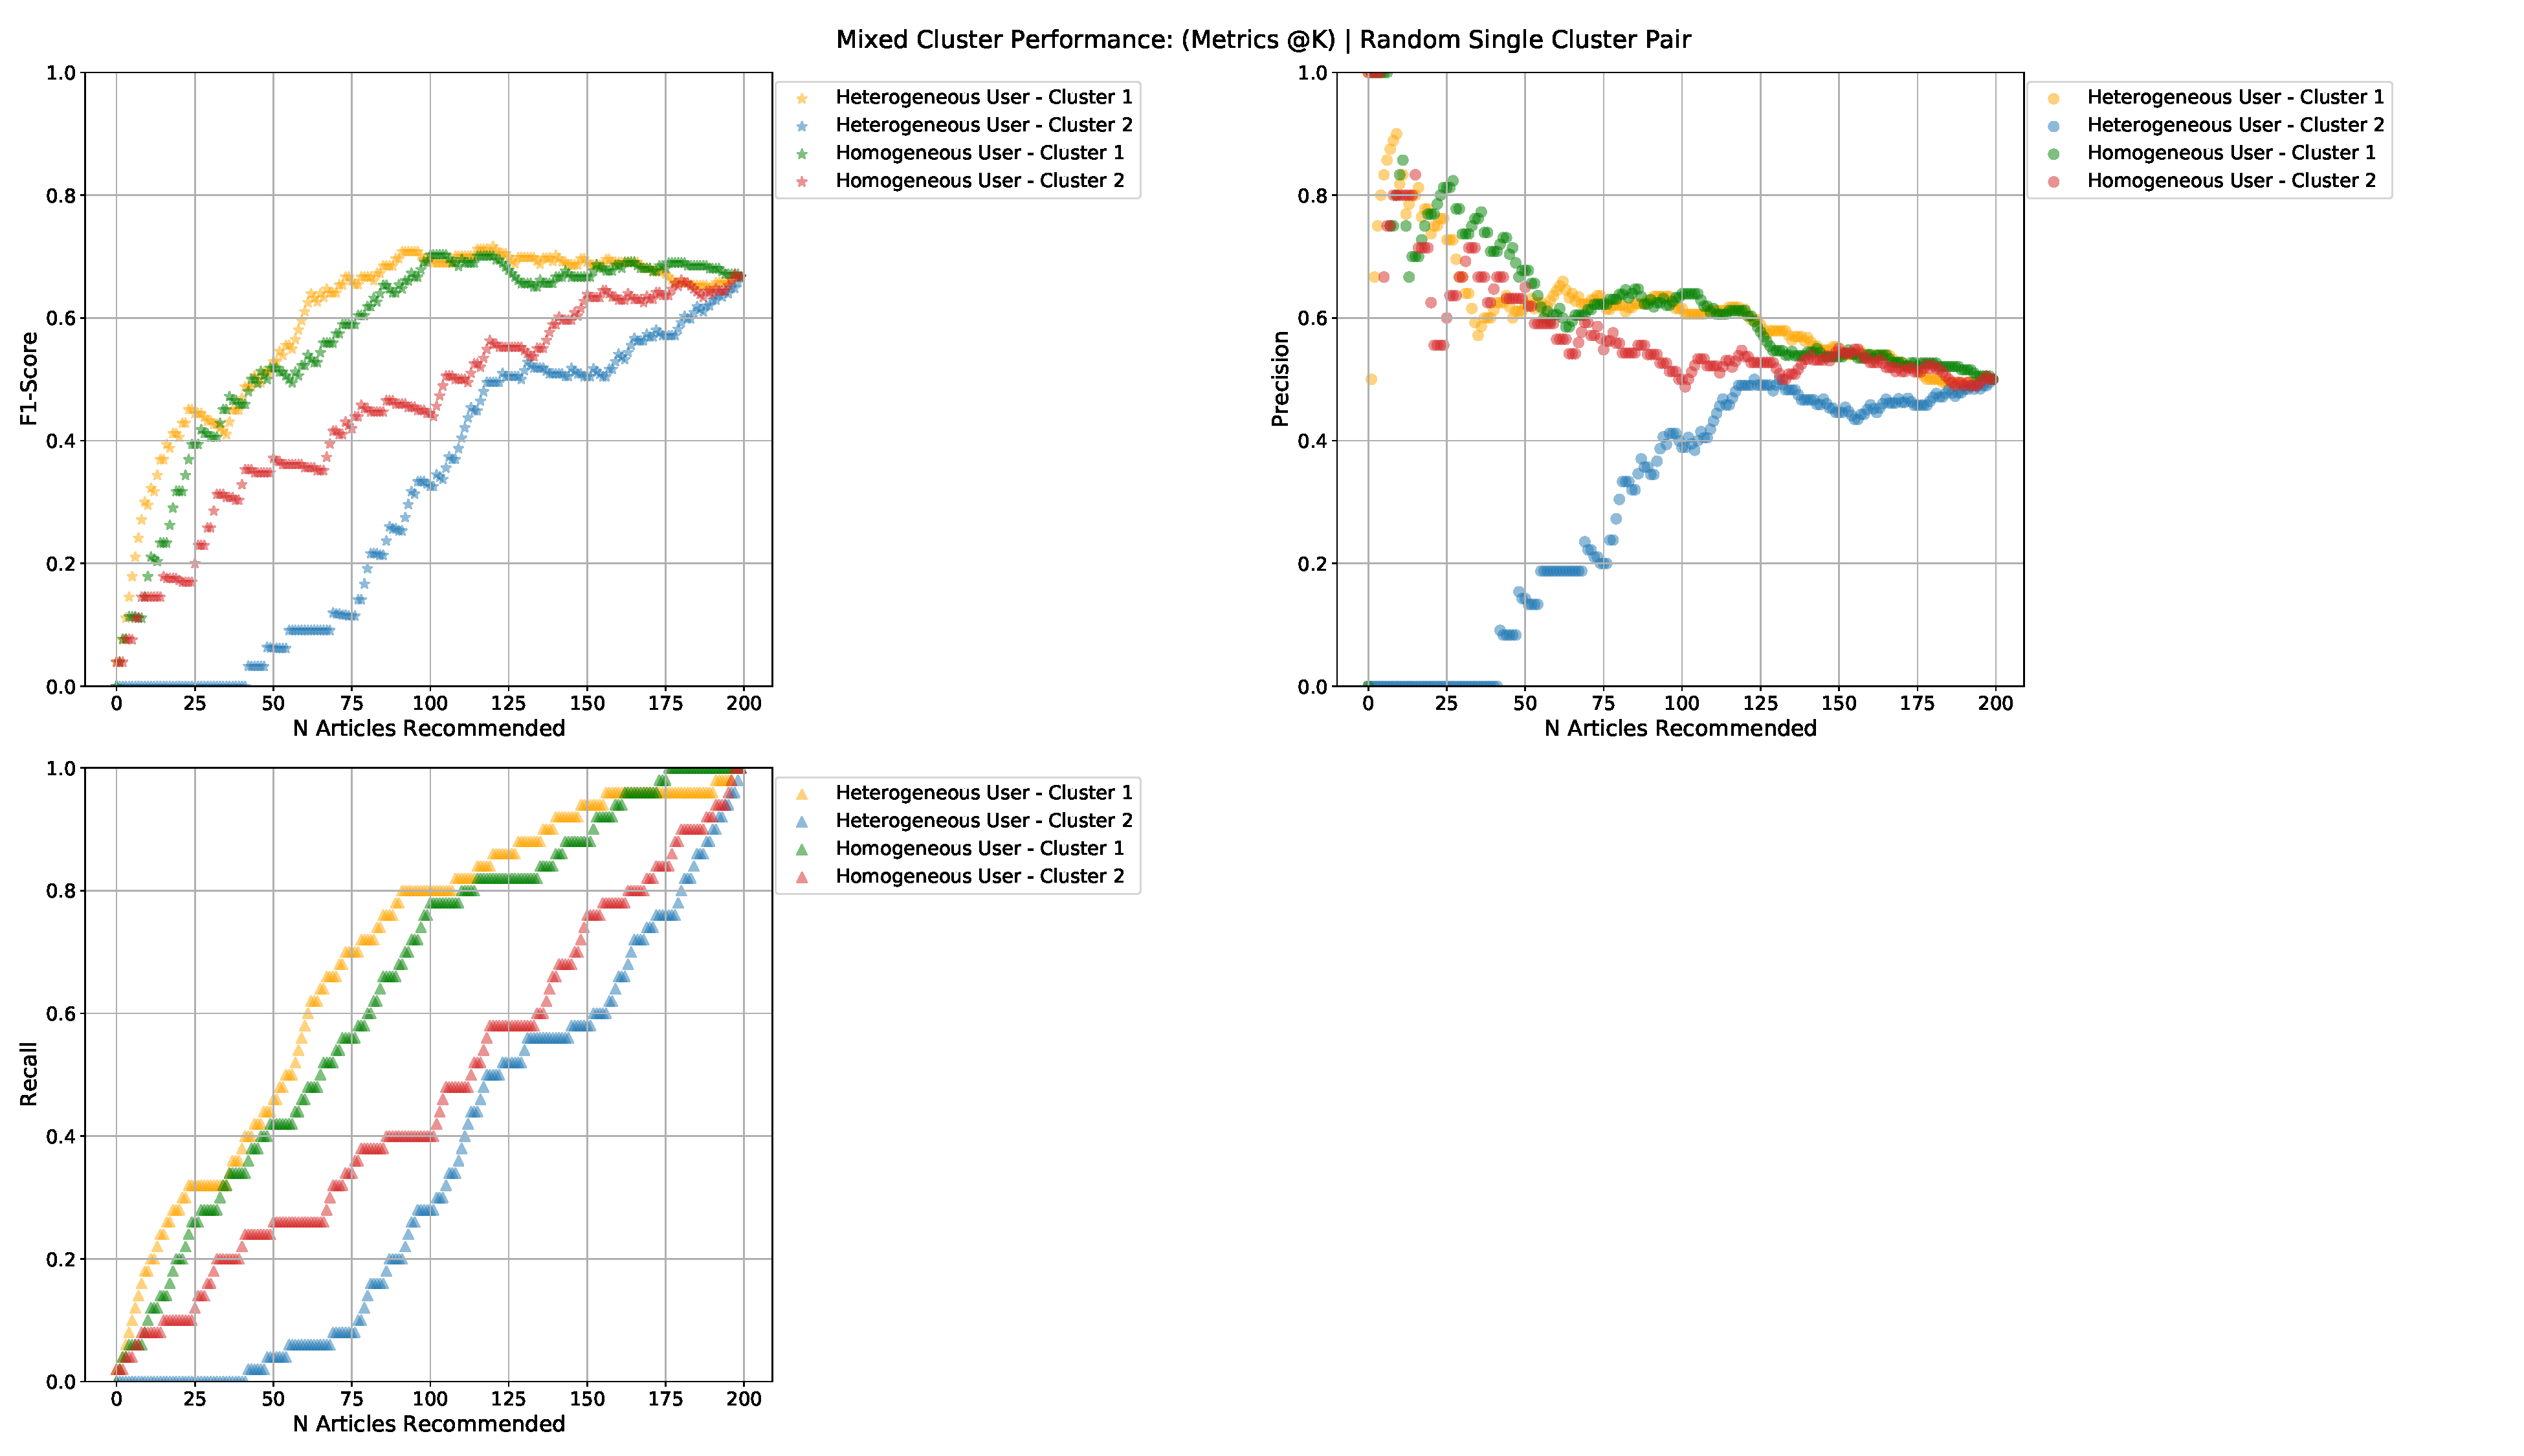
\includegraphics[width=1.0\textwidth]{Graphs/GLOVE/user_interaction_vs_model_performance_mixed_cluster.pdf}
    % \caption{Caption}
    % \label{fig:my_label}
\end{figure}
\begin{figure}[H]
 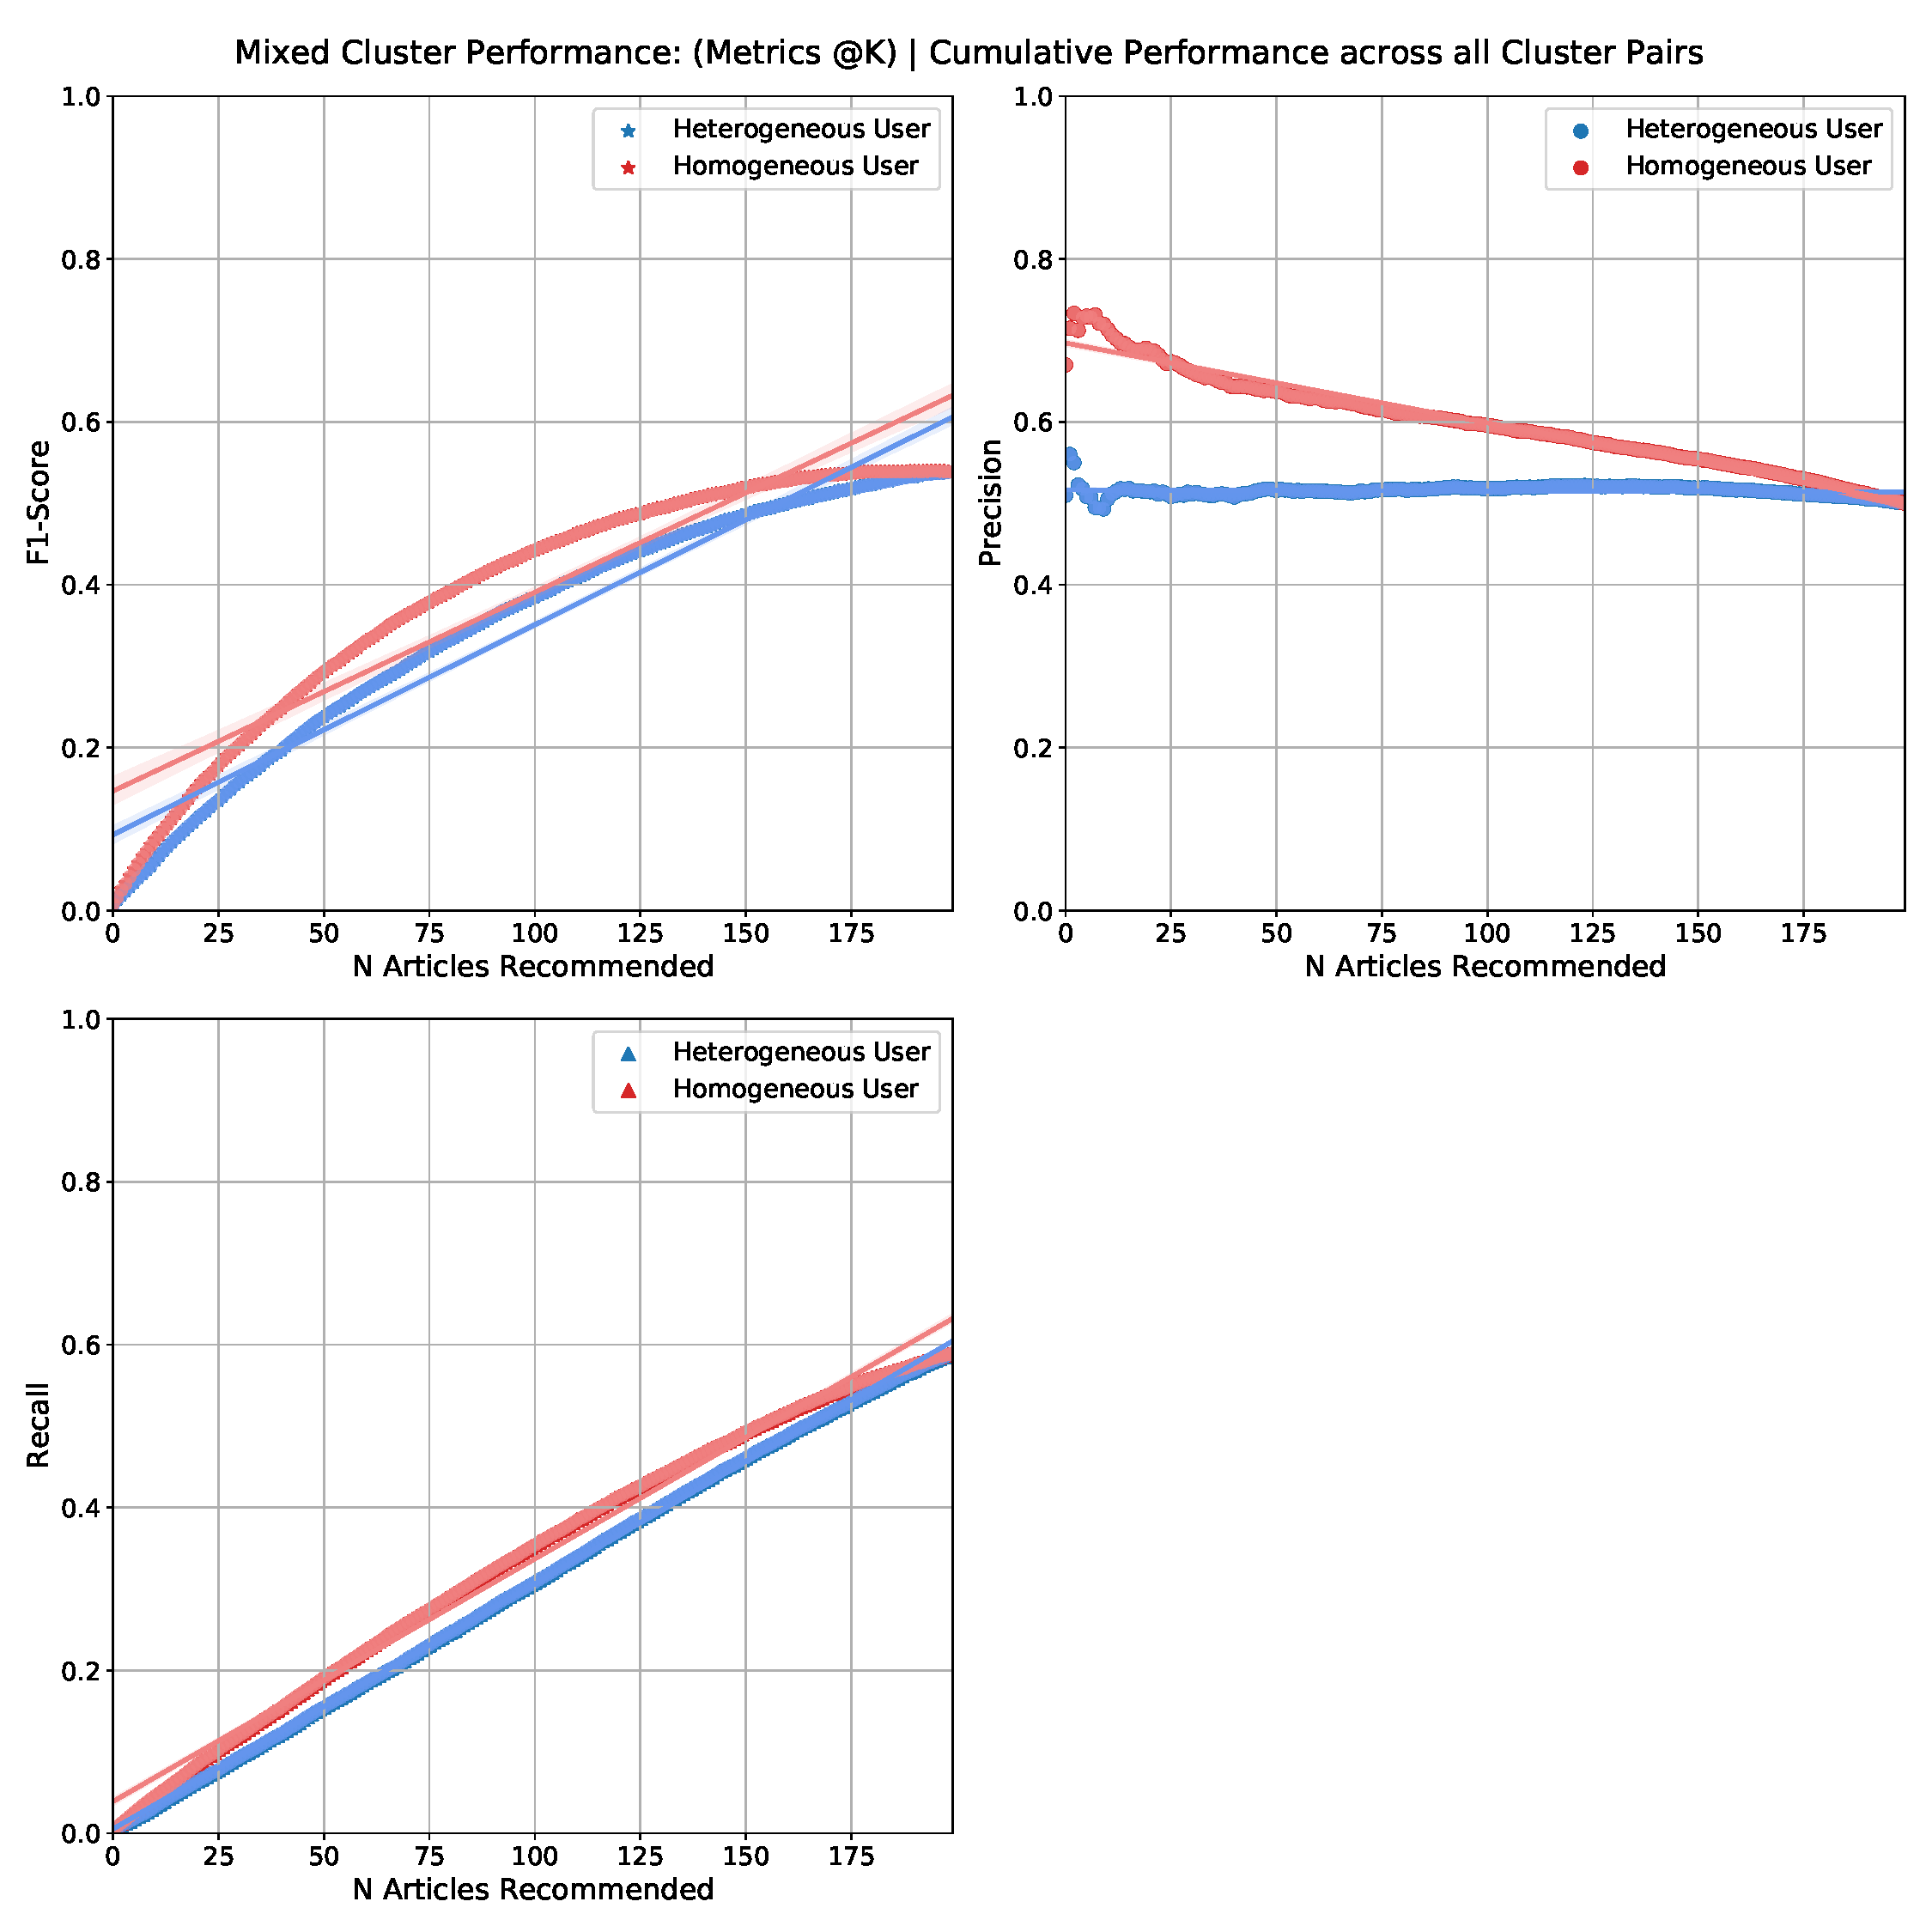
\includegraphics[width=0.6\textwidth]{Graphs/GLOVE/user_interaction_vs_model_performance_cumu_mixed_cluster.pdf}
\end{figure}
\begin{figure}[H]
 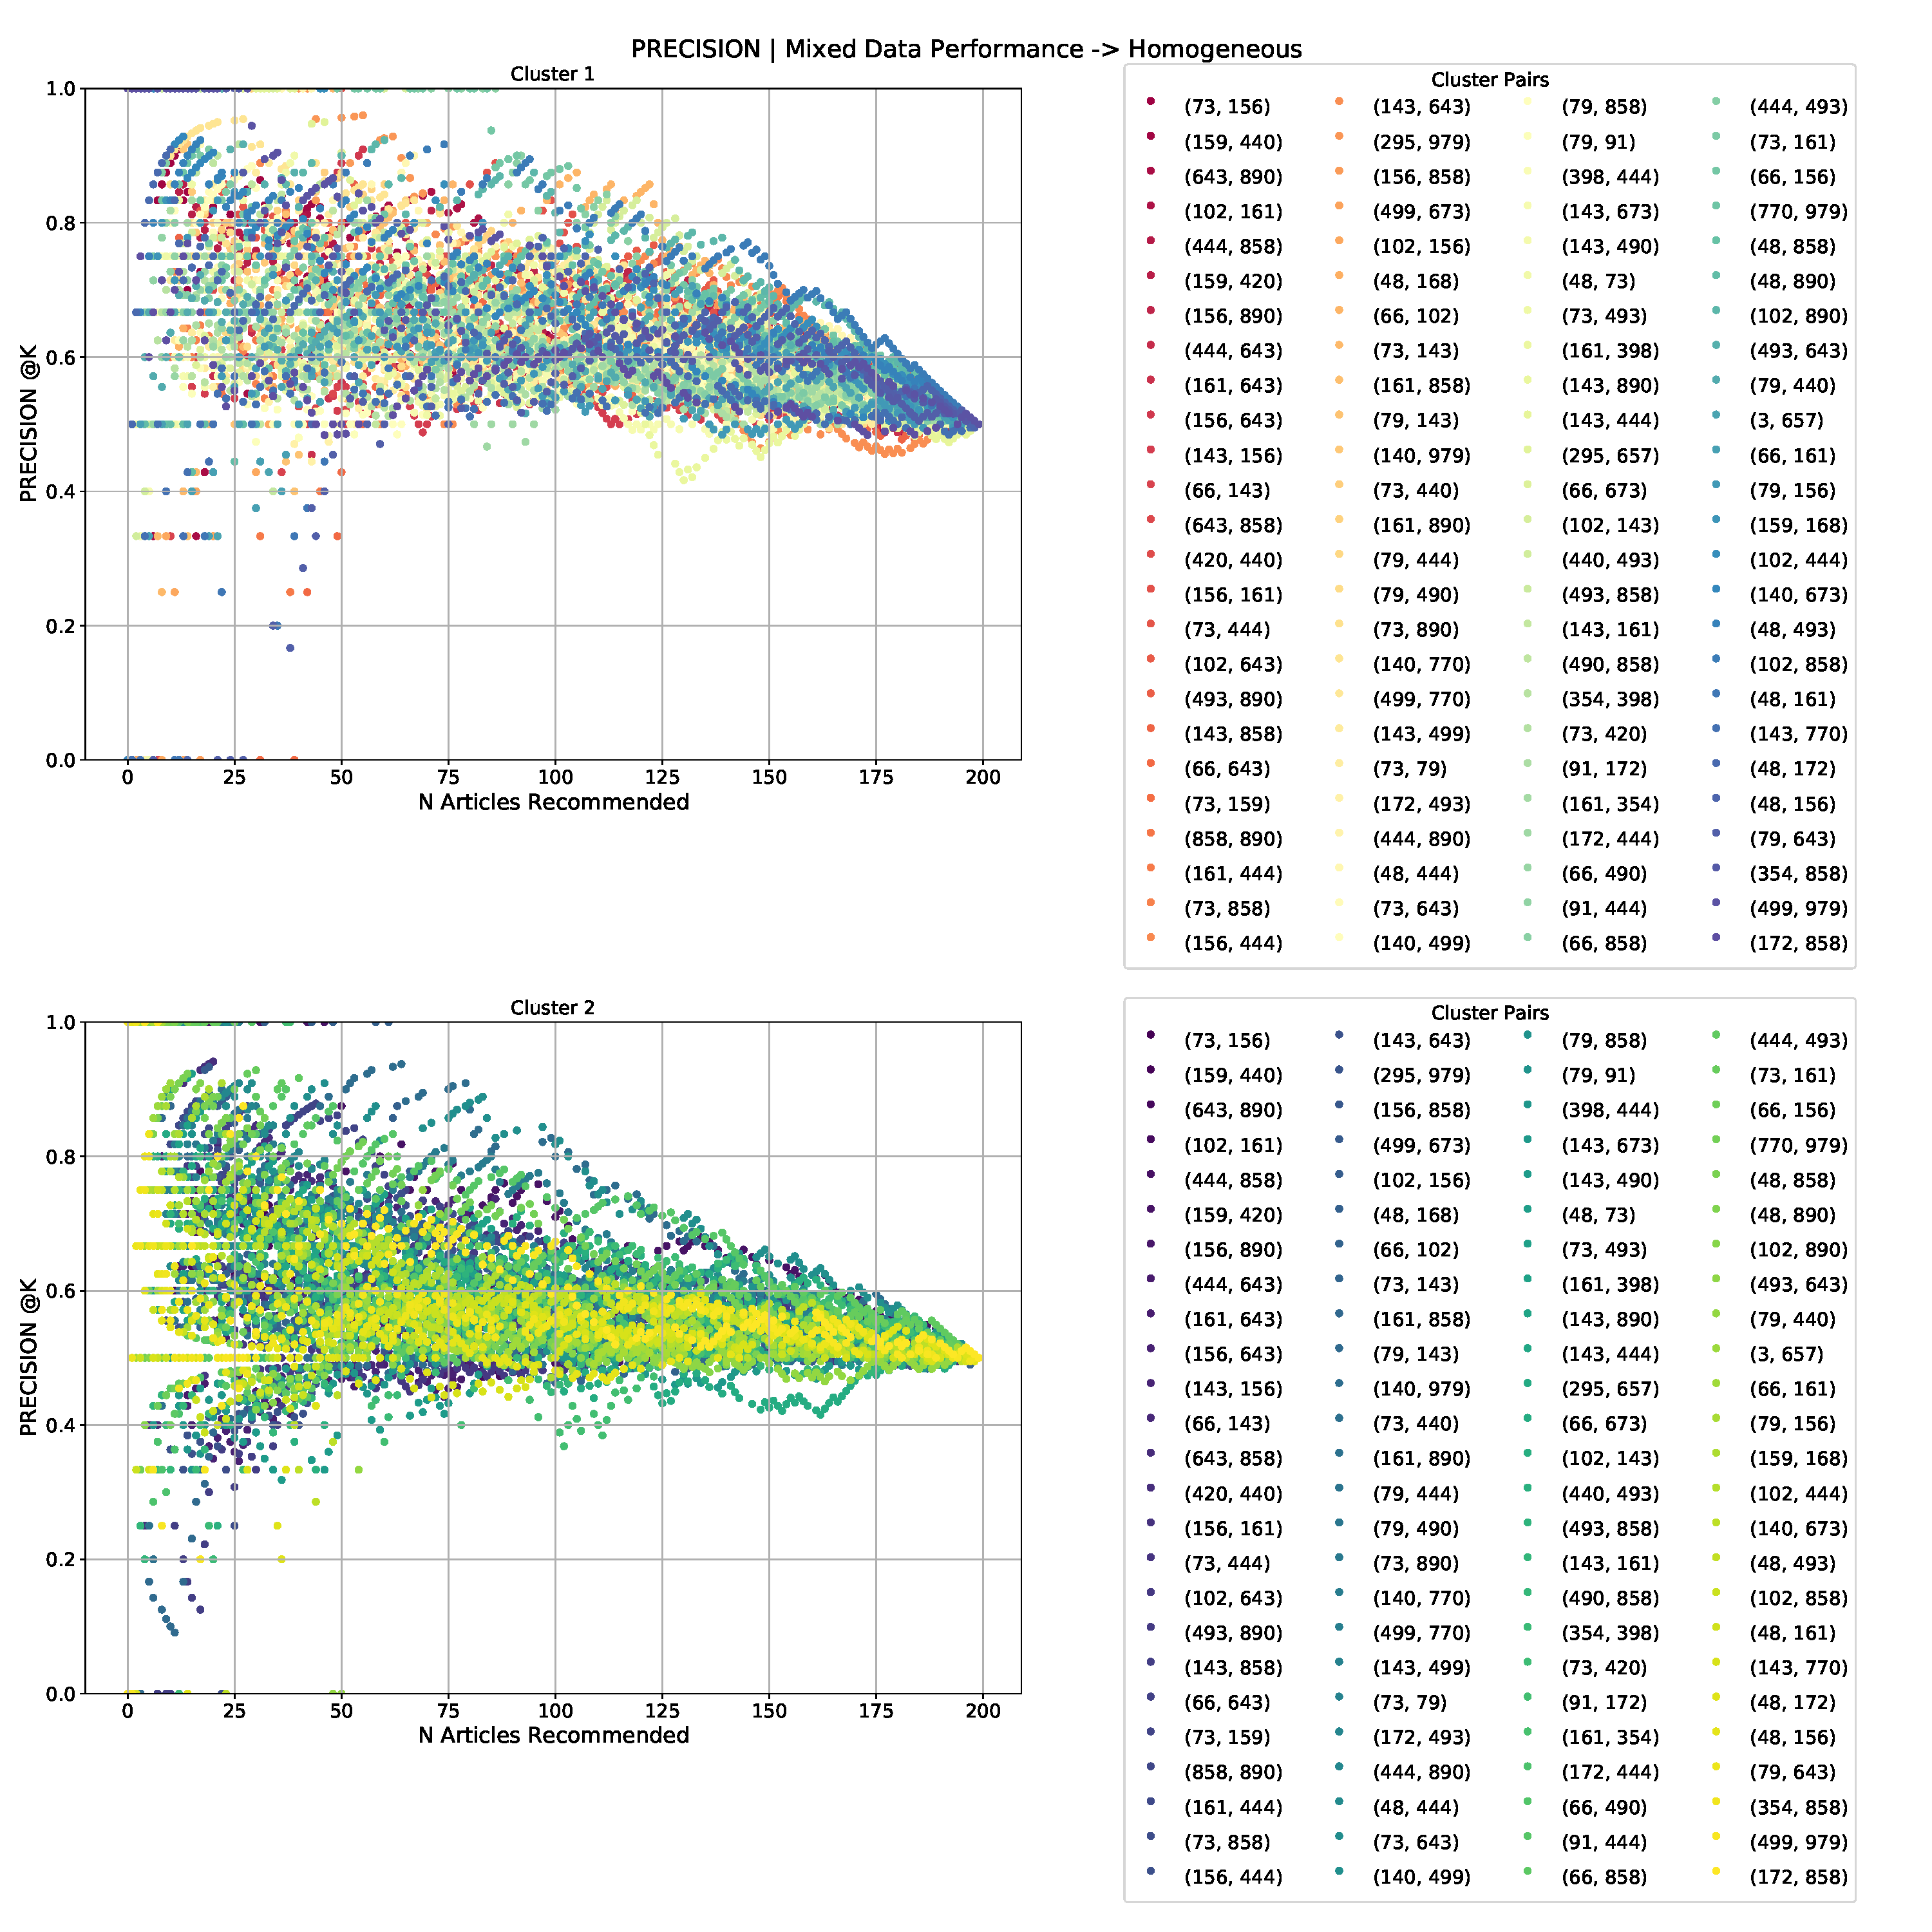
\includegraphics[width=0.7\textwidth]{Graphs/GLOVE/user_interaction_vs_model_performance_precision_all_cps_mixed_data_sep_Homogeneous.pdf}
\end{figure}
\begin{figure}[H]
 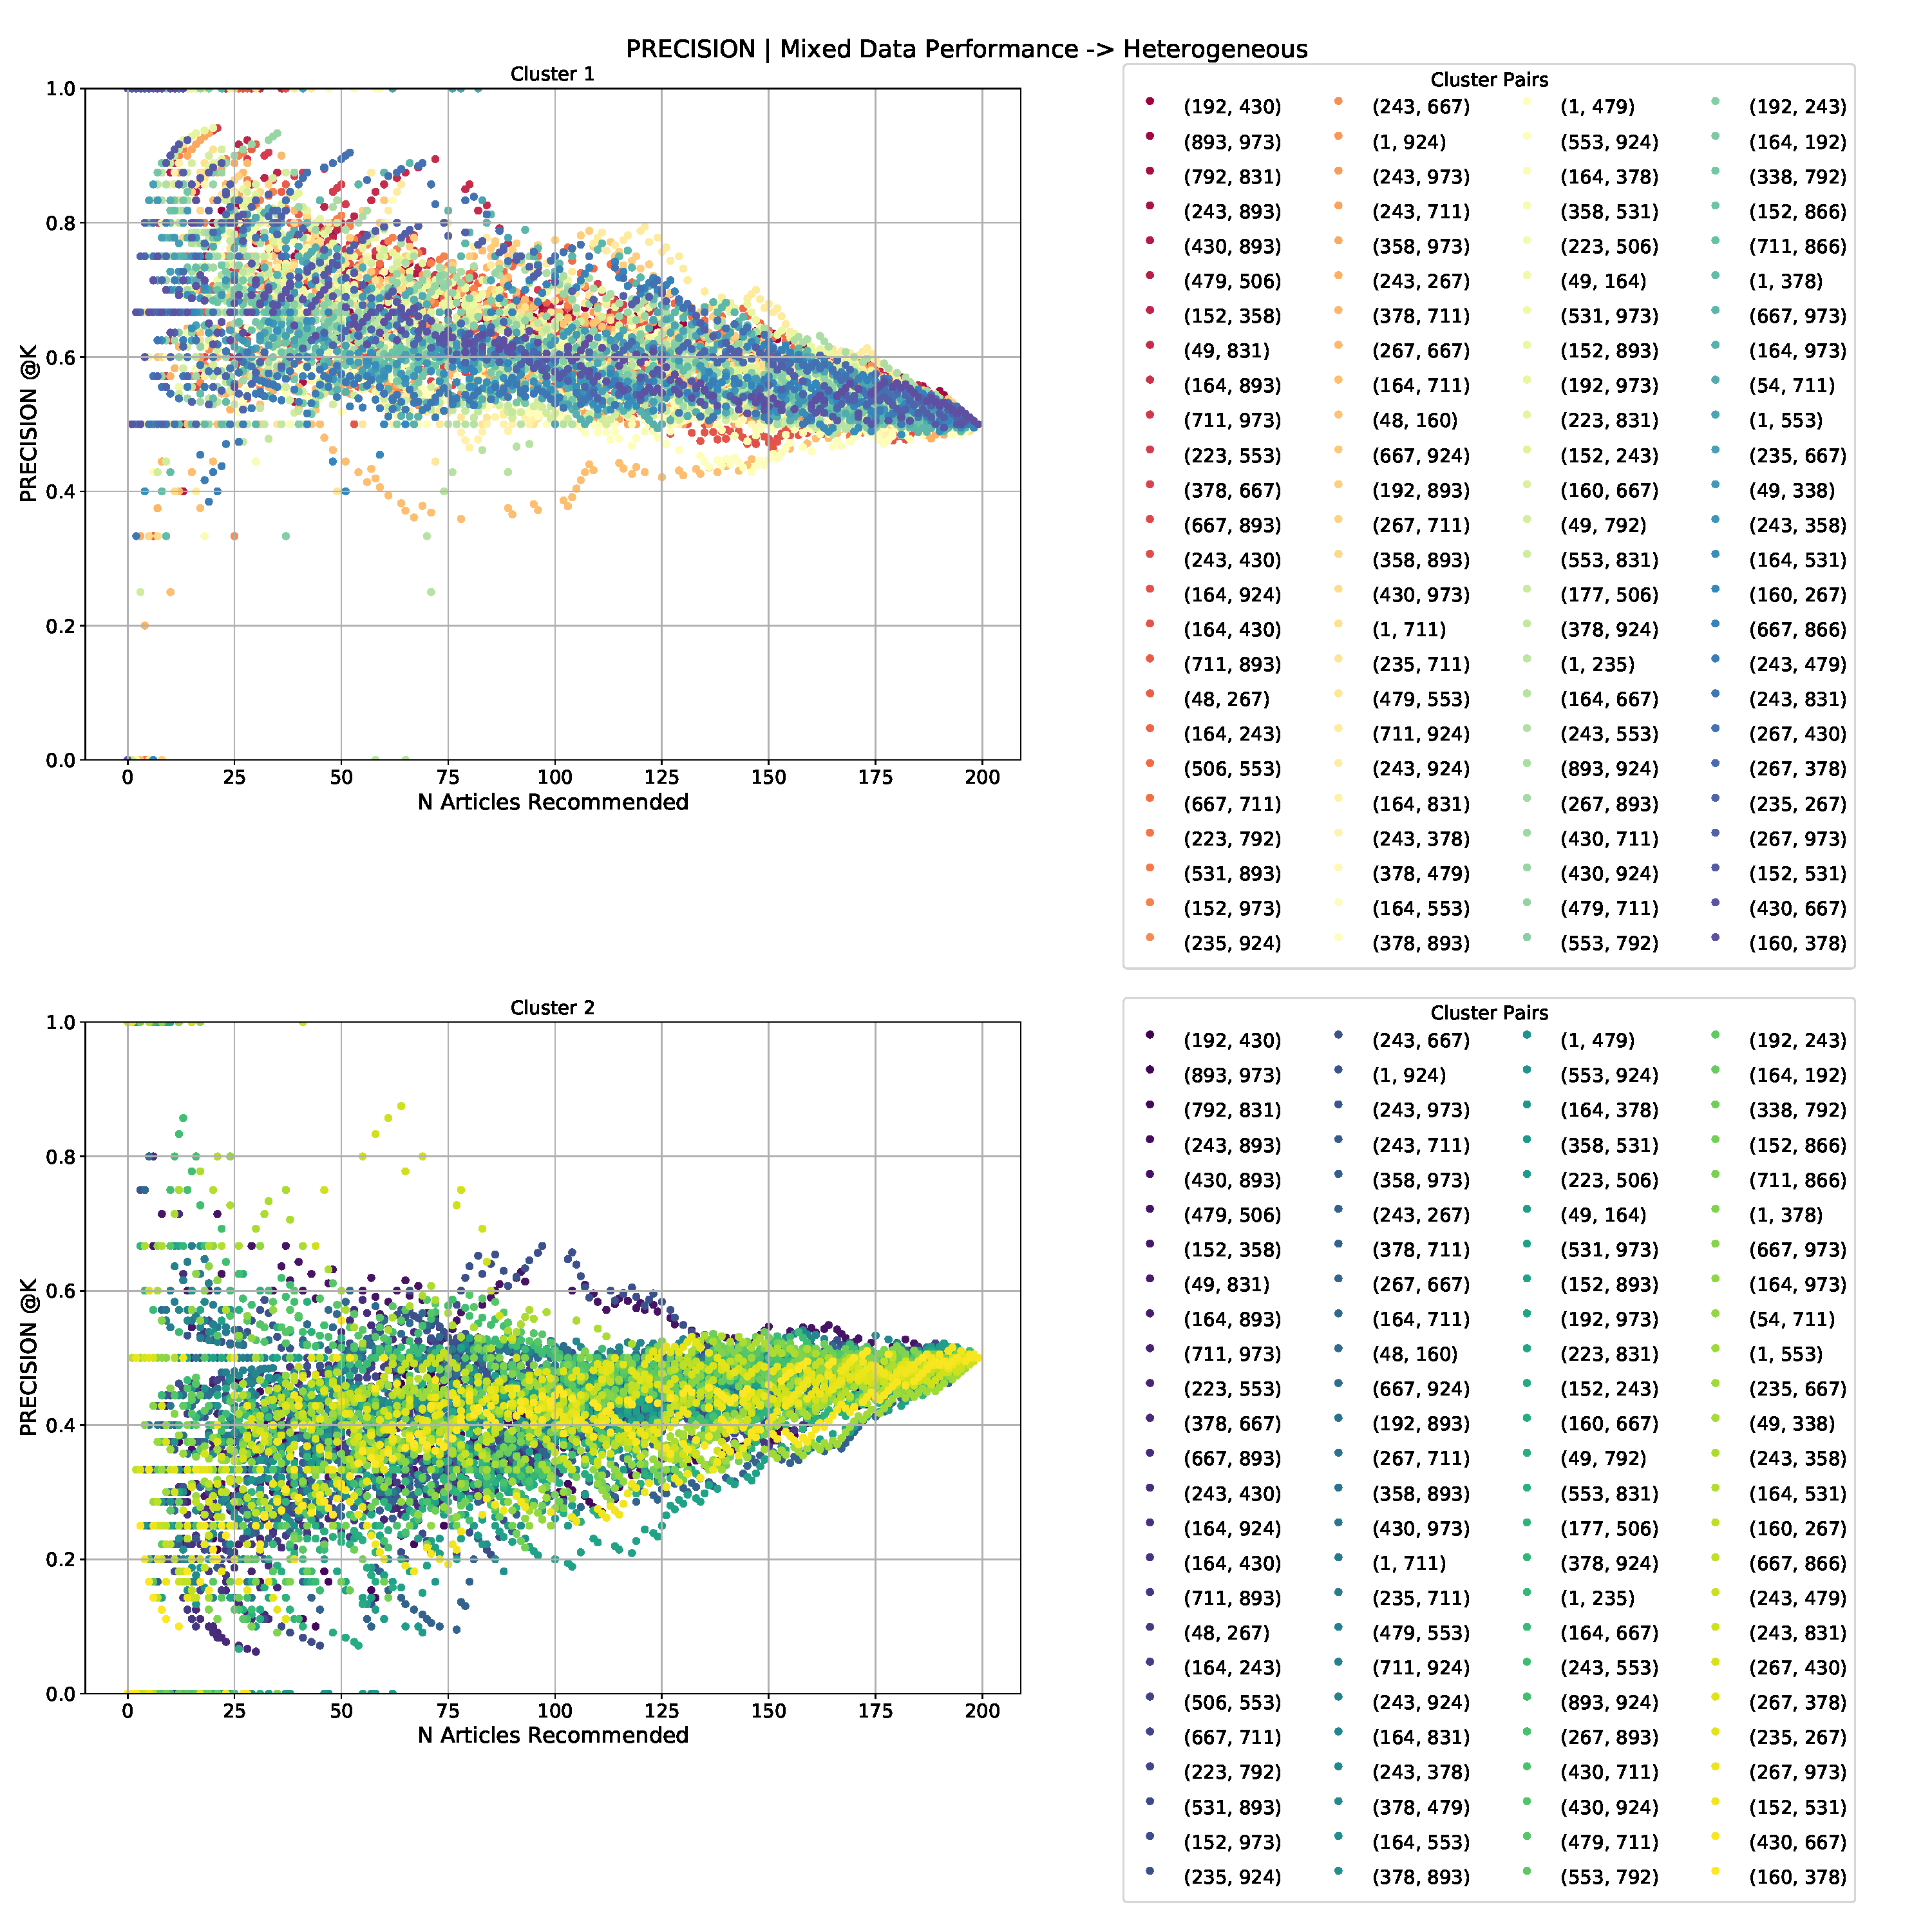
\includegraphics[width=0.7\textwidth]{Graphs/GLOVE/user_interaction_vs_model_performance_precision_all_cps_mixed_data_sep_Heterogeneous.pdf}
\end{figure}
\subsection{BERT}
\begin{figure}[H]
    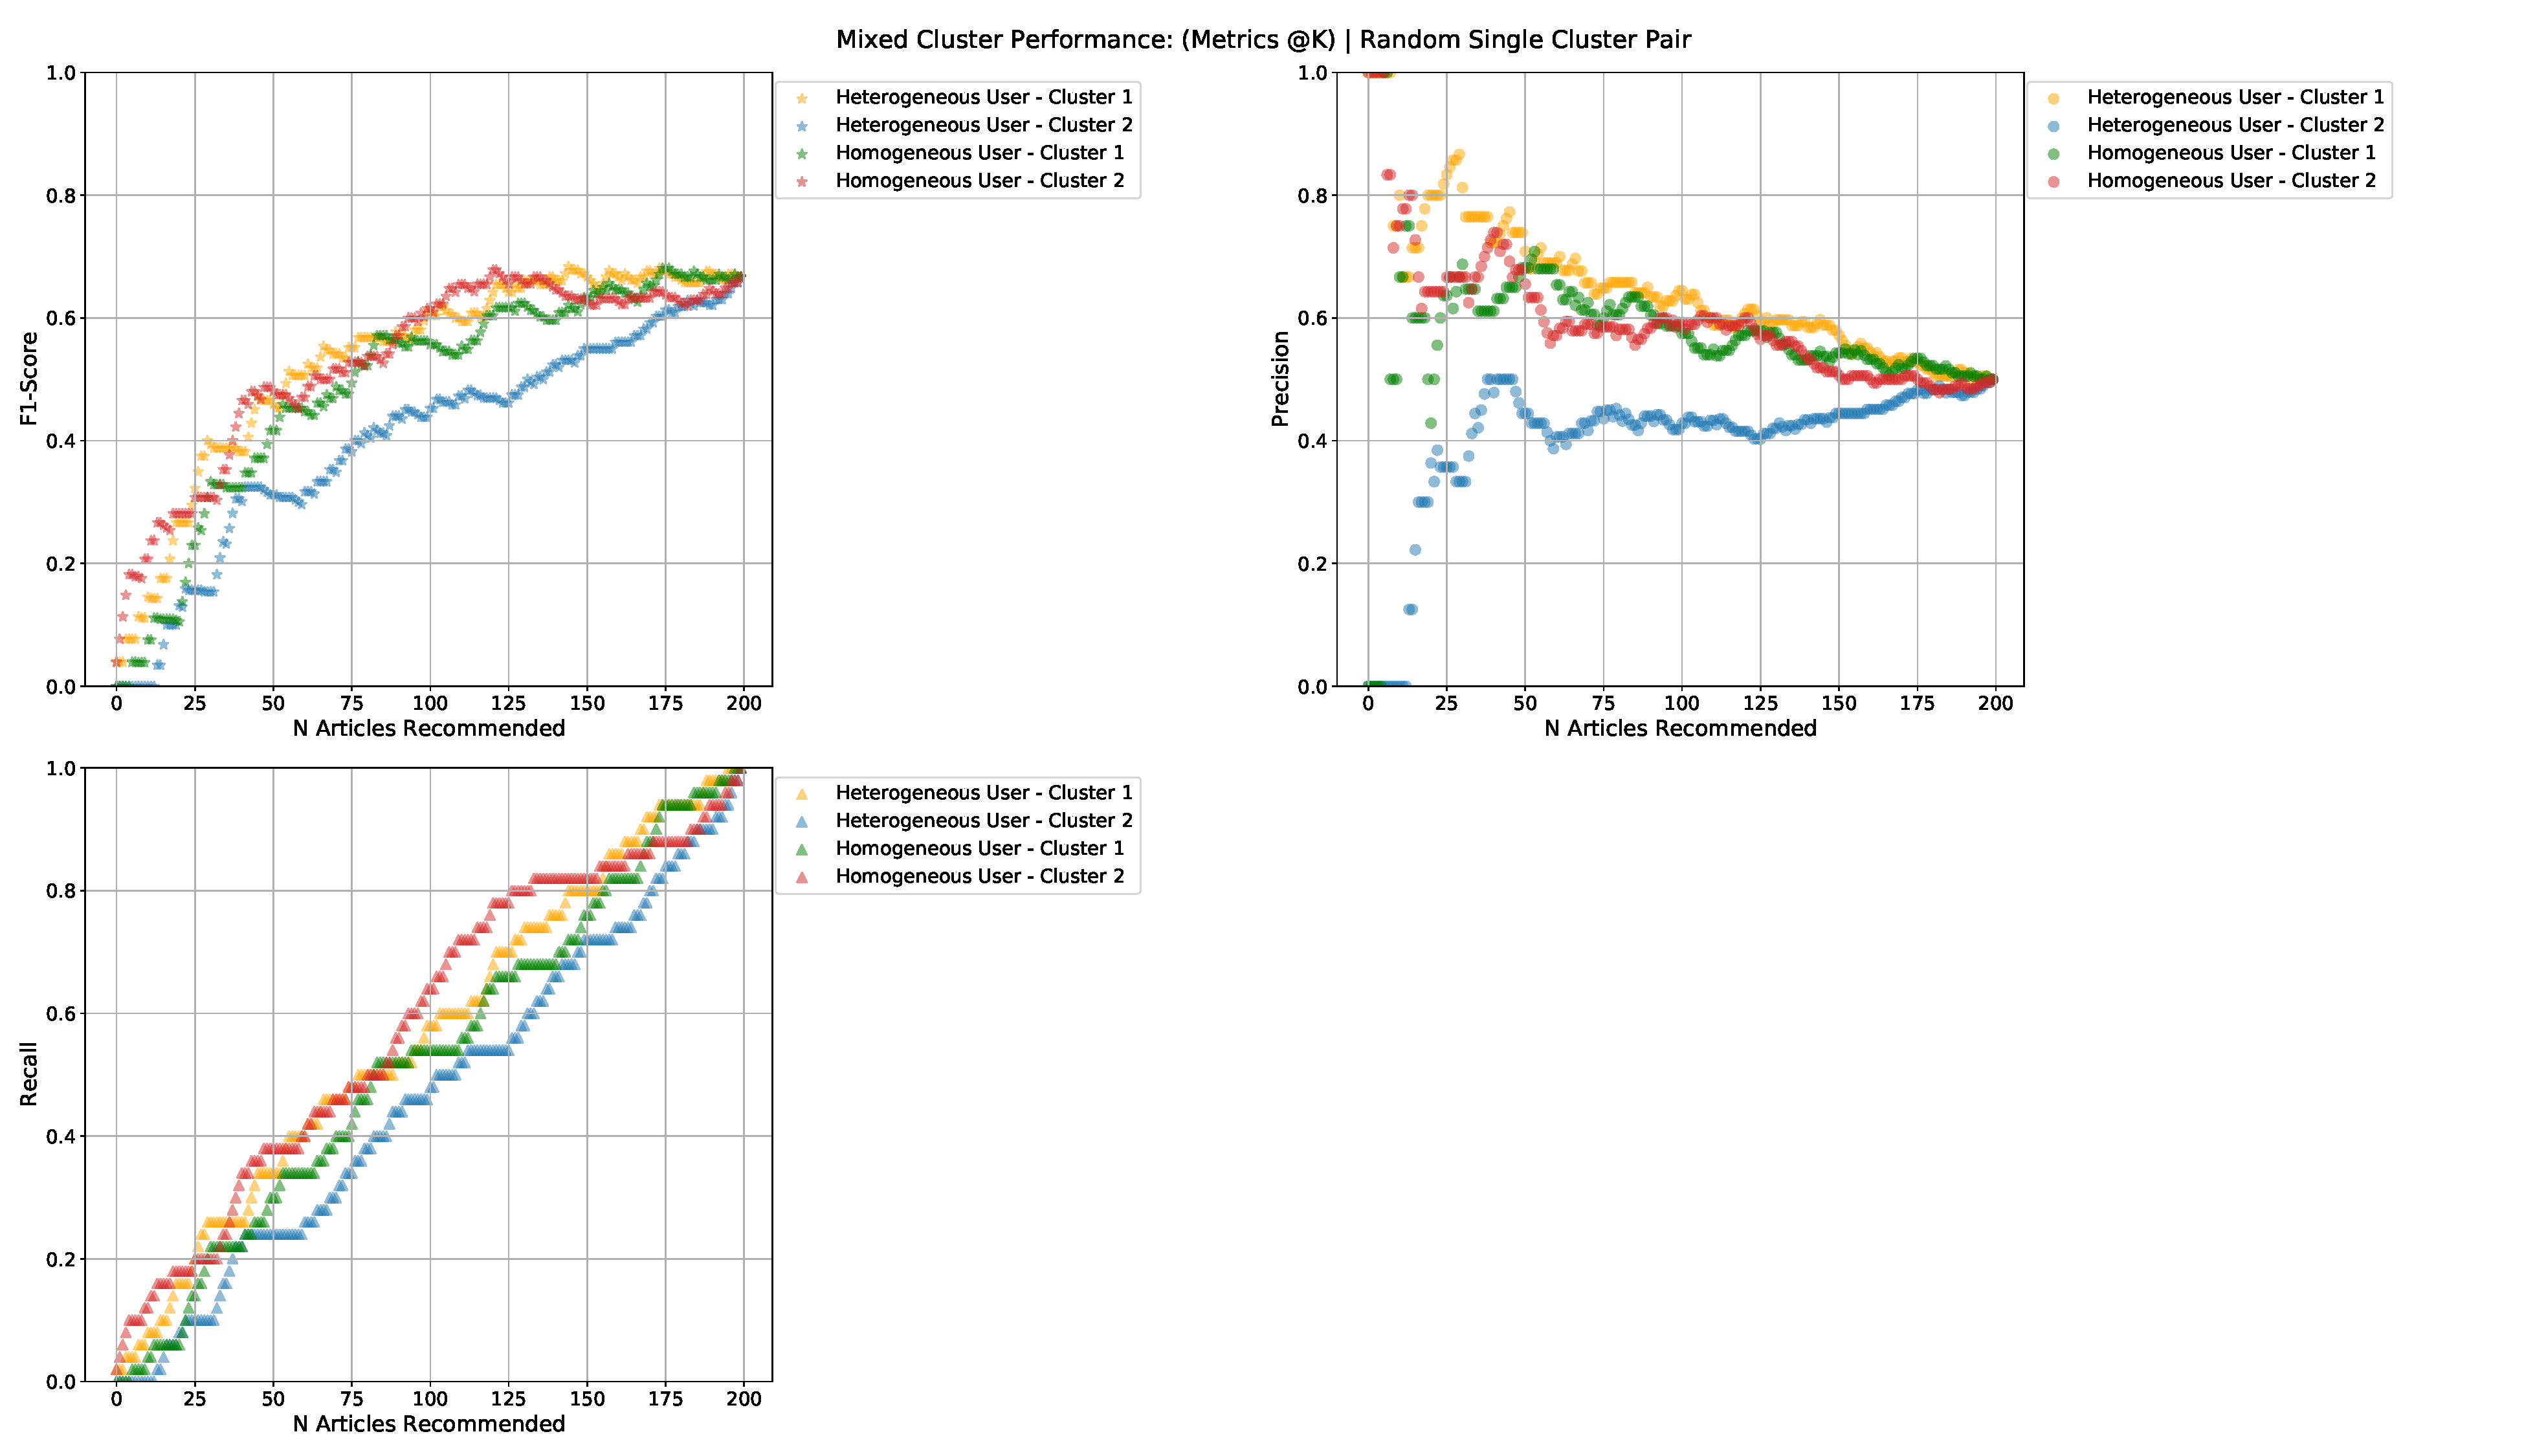
\includegraphics[width=1.0\textwidth]{Graphs/BERT/user_interaction_vs_model_performance_mixed_cluster.pdf}
    % \caption{Caption}
    % \label{fig:my_label}
\end{figure}
\begin{figure}[H]
 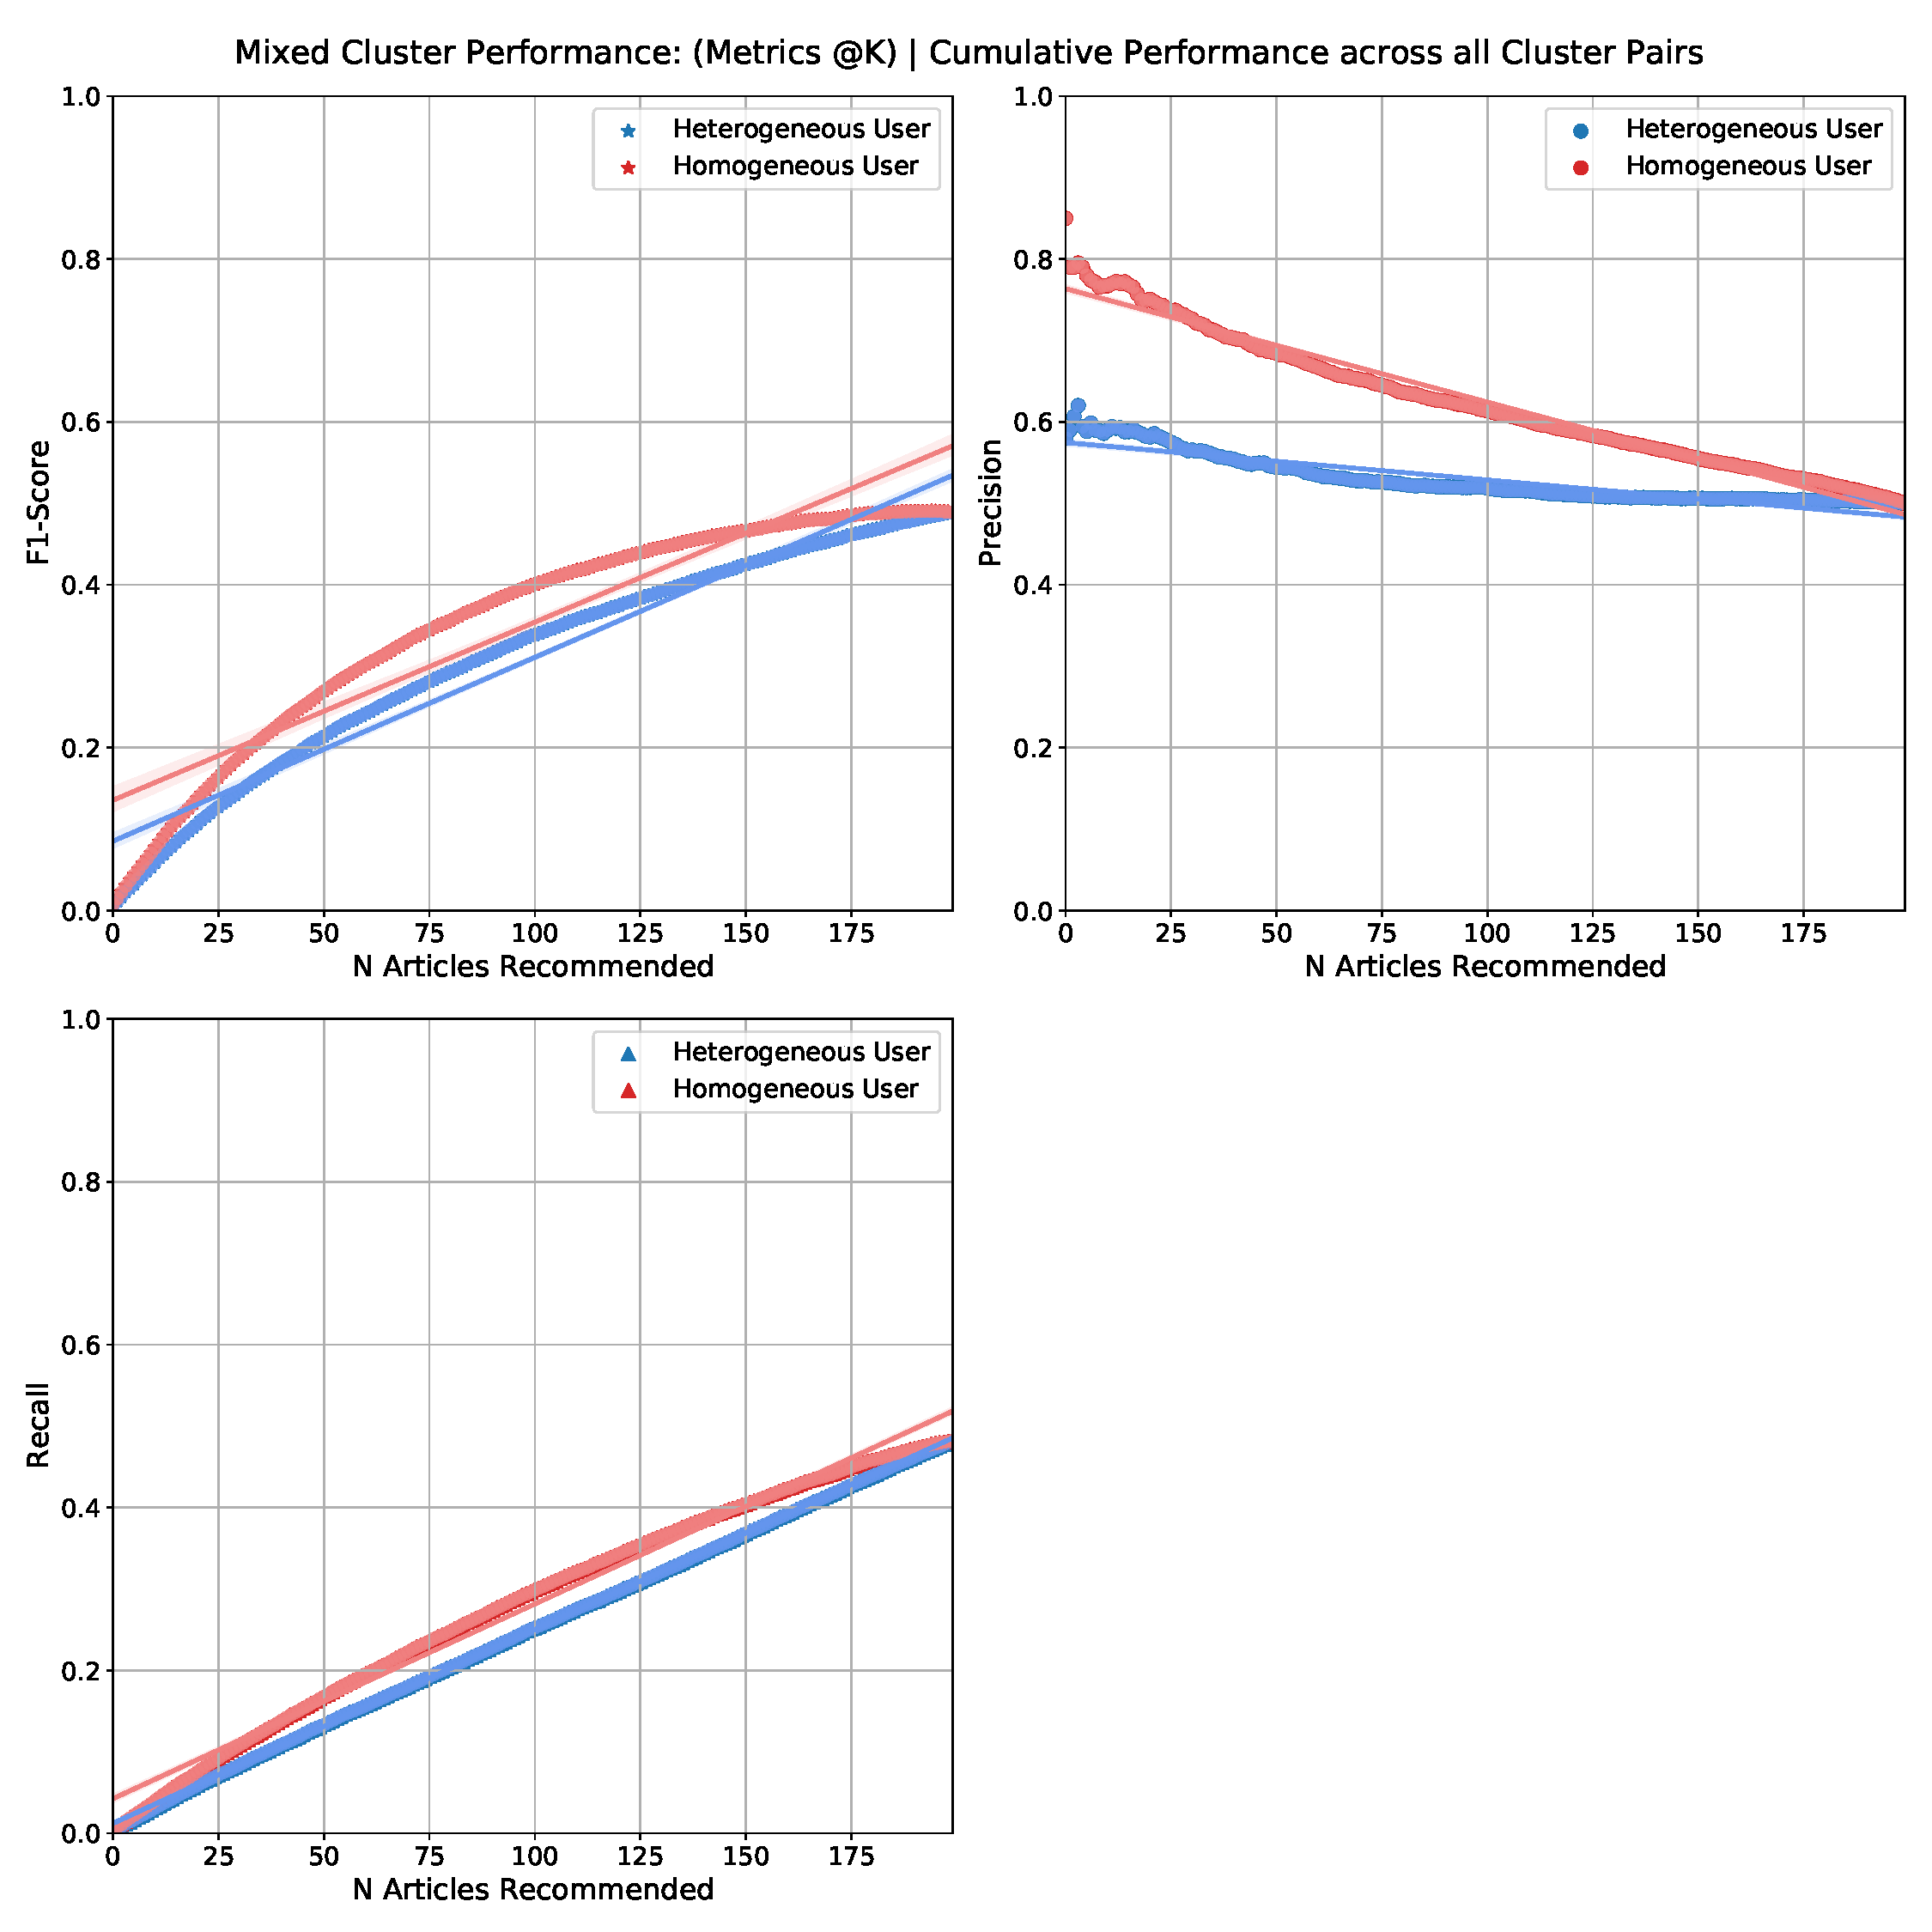
\includegraphics[width=0.6\textwidth]{Graphs/BERT/user_interaction_vs_model_performance_cumu_mixed_cluster.pdf}
\end{figure}
\begin{figure}[H]
 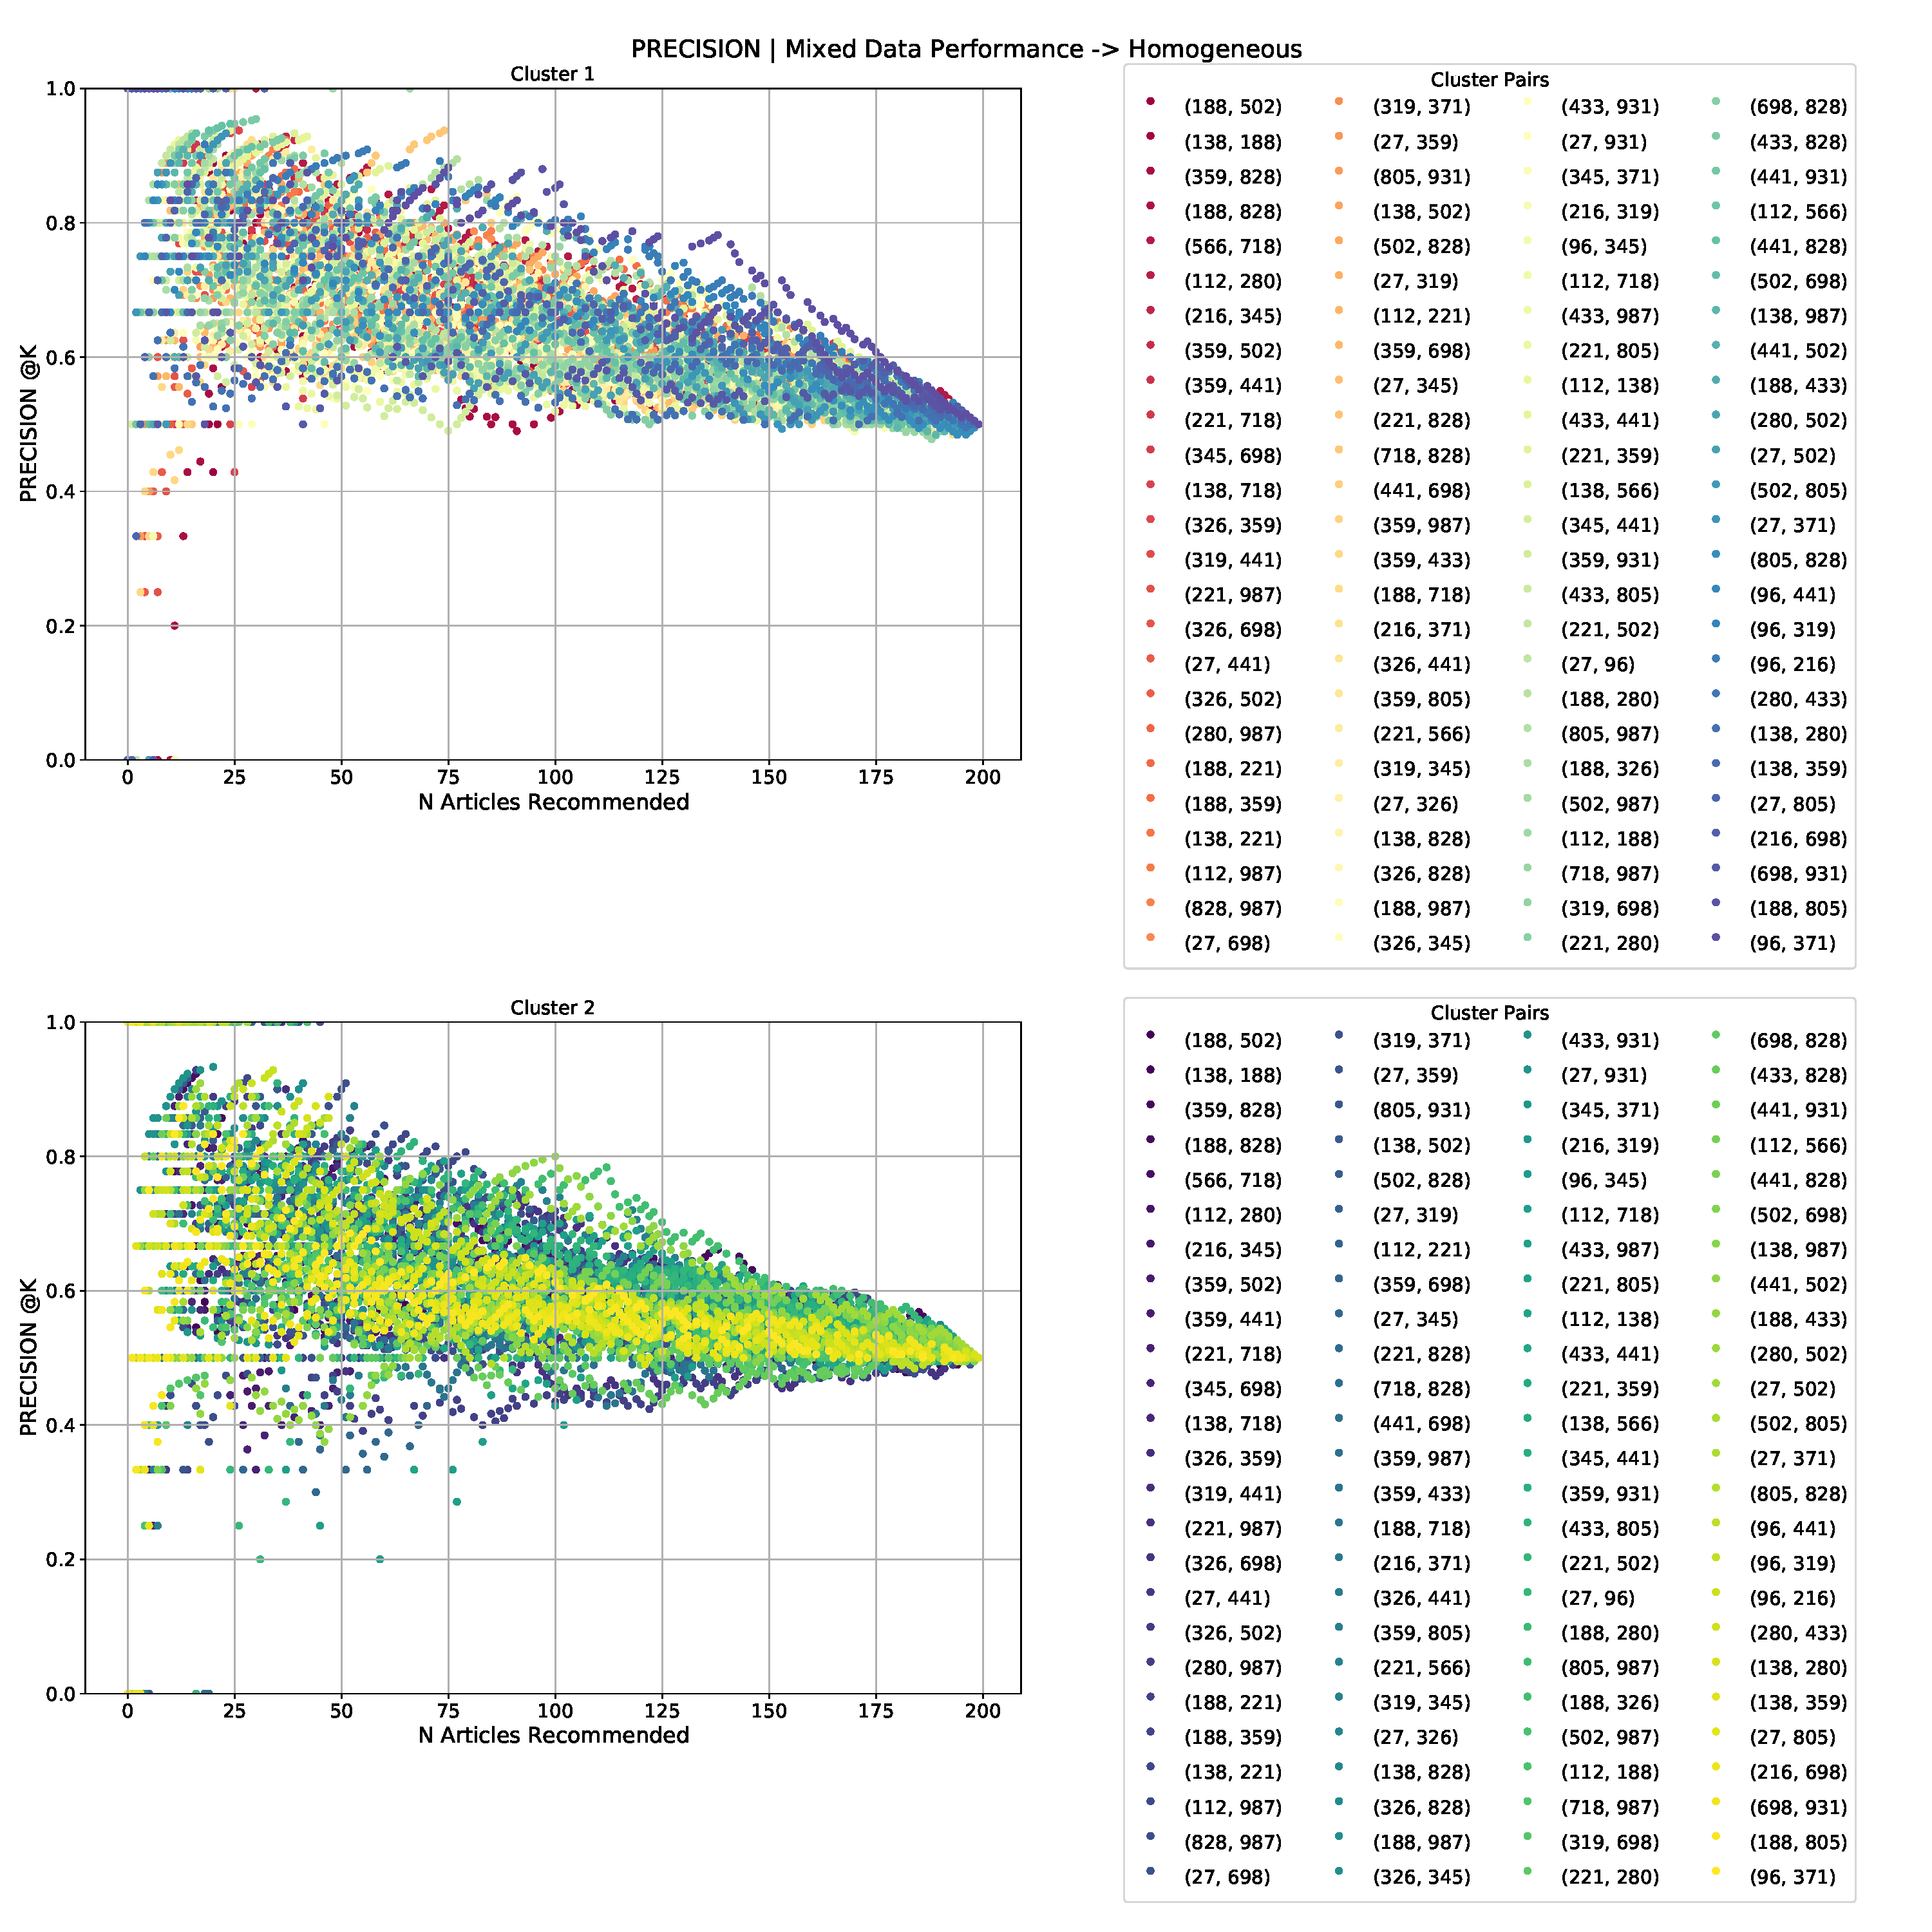
\includegraphics[width=0.7\textwidth]{Graphs/BERT/user_interaction_vs_model_performance_precision_all_cps_mixed_data_sep_Homogeneous.pdf}
\end{figure}
\begin{figure}[H]
 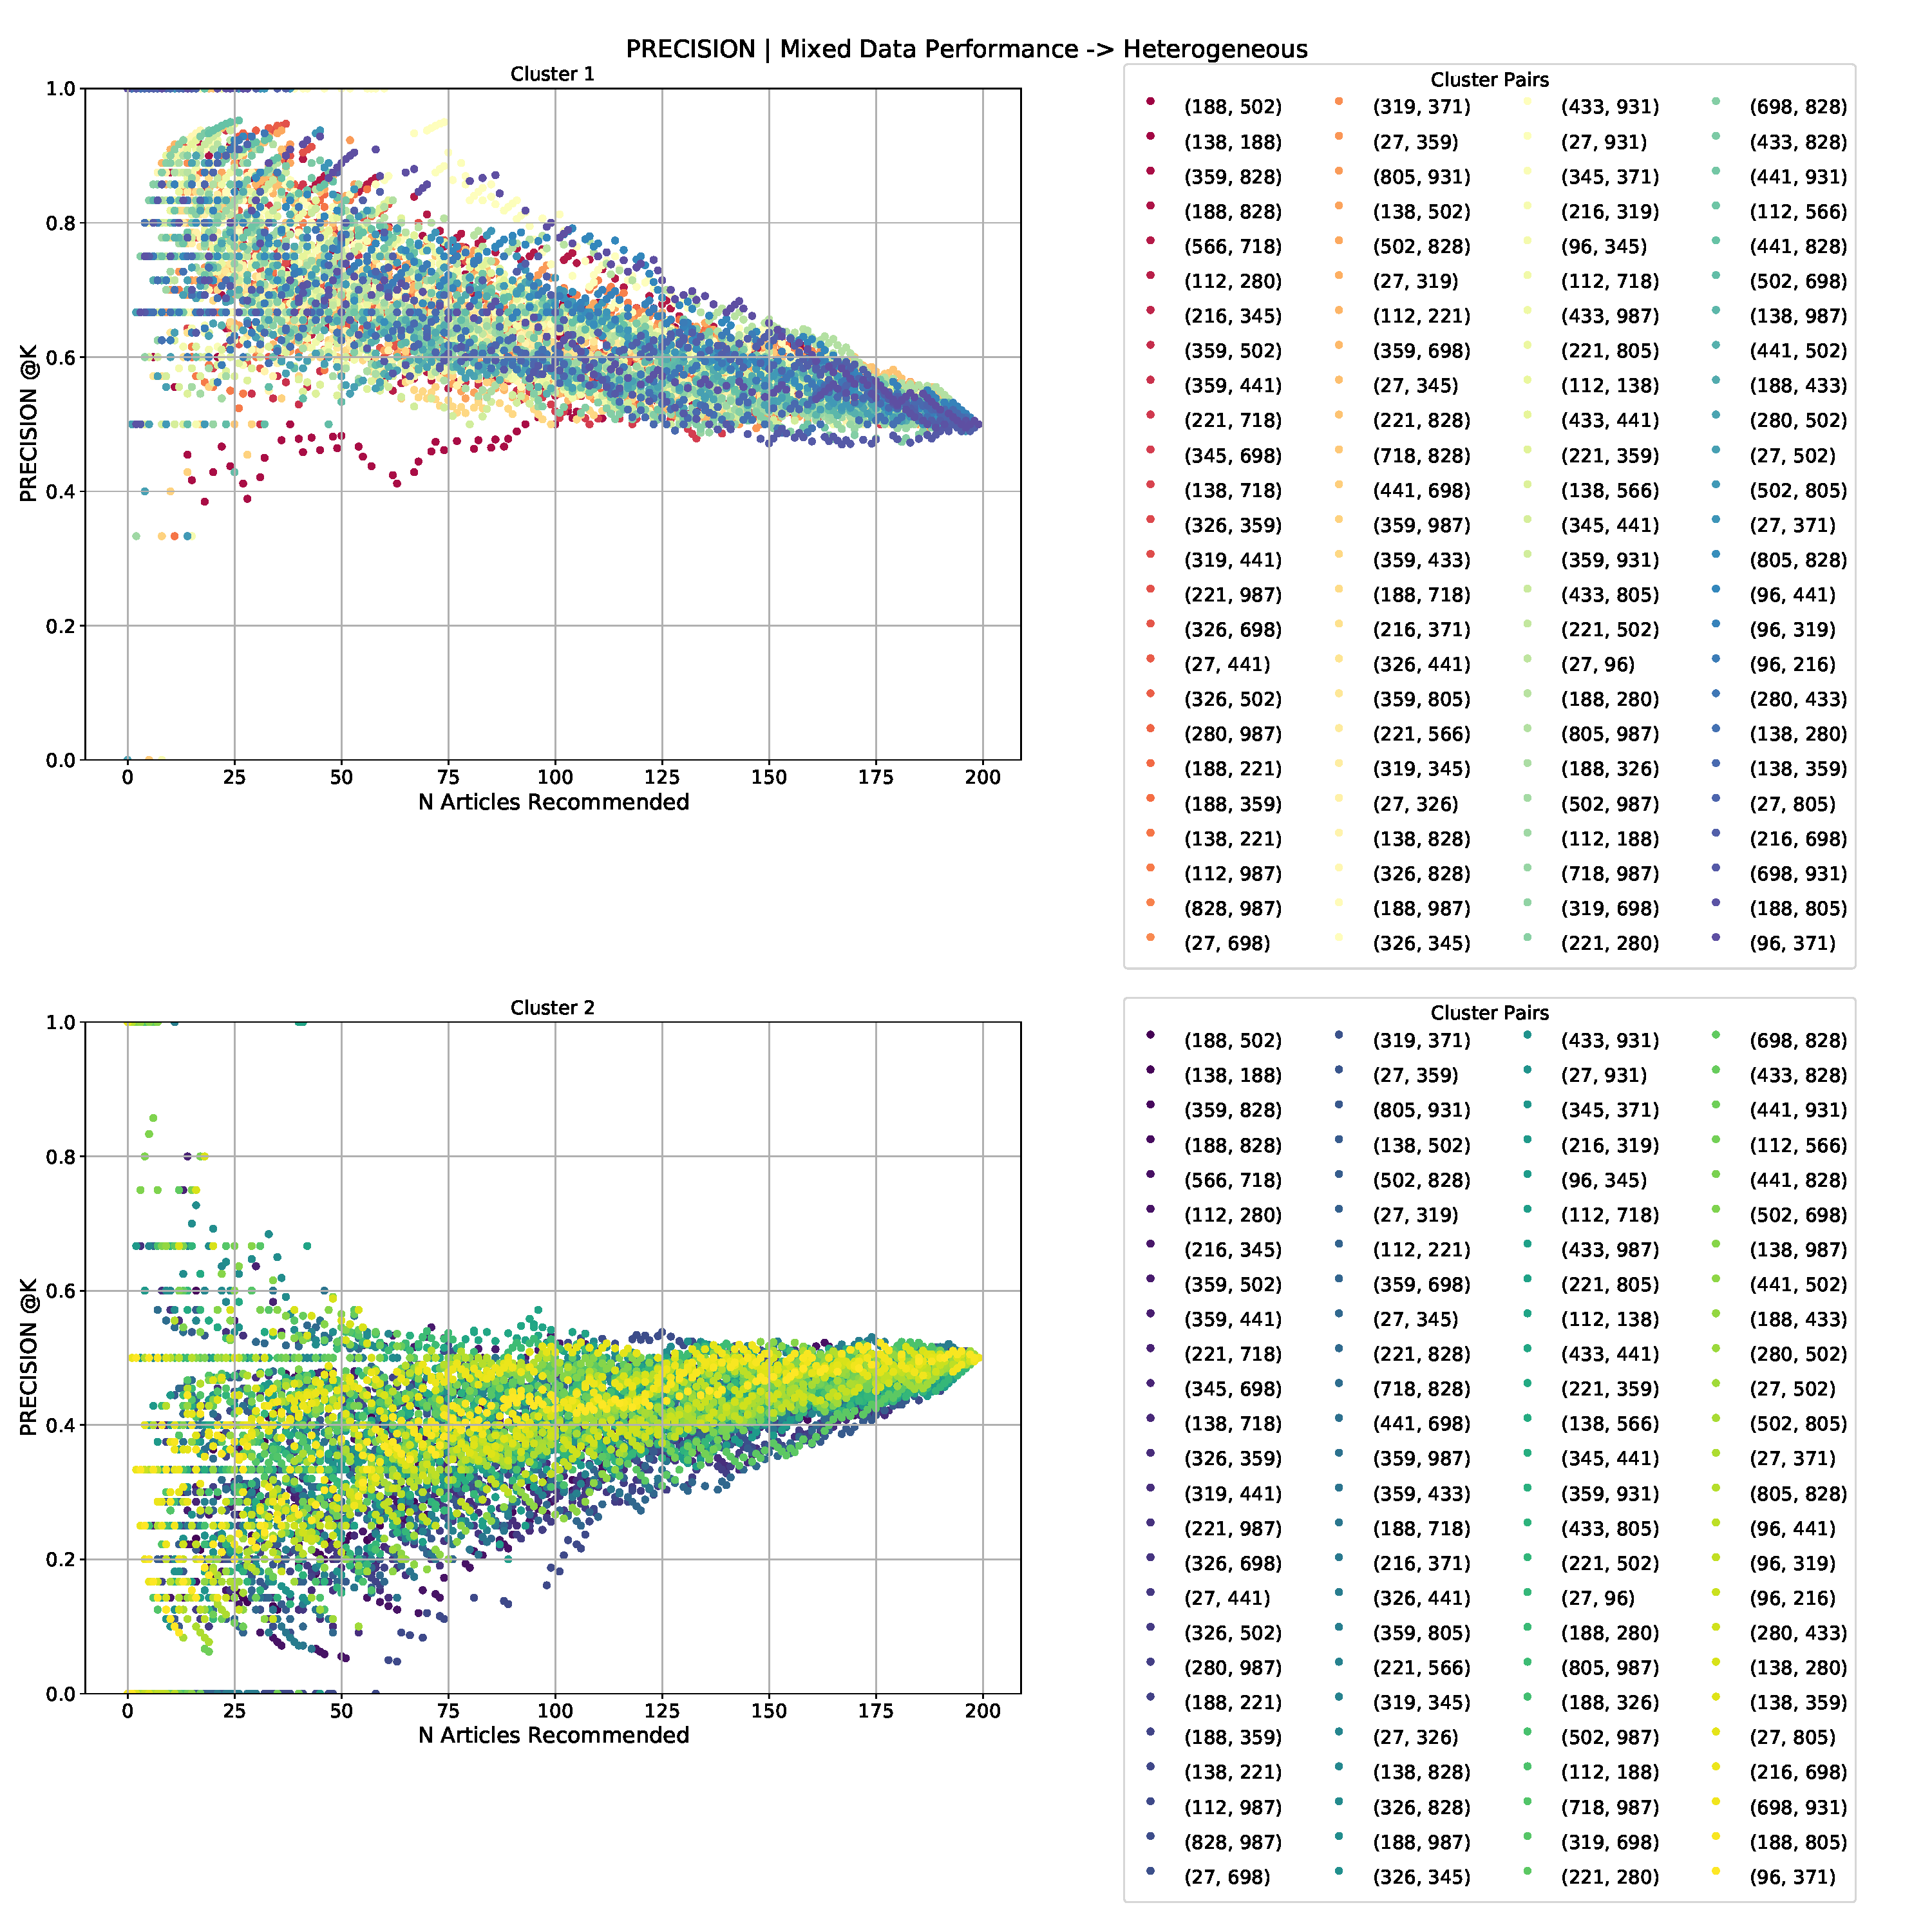
\includegraphics[width=0.7\textwidth]{Graphs/BERT/user_interaction_vs_model_performance_precision_all_cps_mixed_data_sep_Heterogeneous.pdf}
\end{figure}


\newpage
\section{Baseline 7: Learning Rate Variation for Mixed Cluster}
\subsection{TF-IDF}
\subsubsection{Homogeneous}
\begin{figure}[H]
    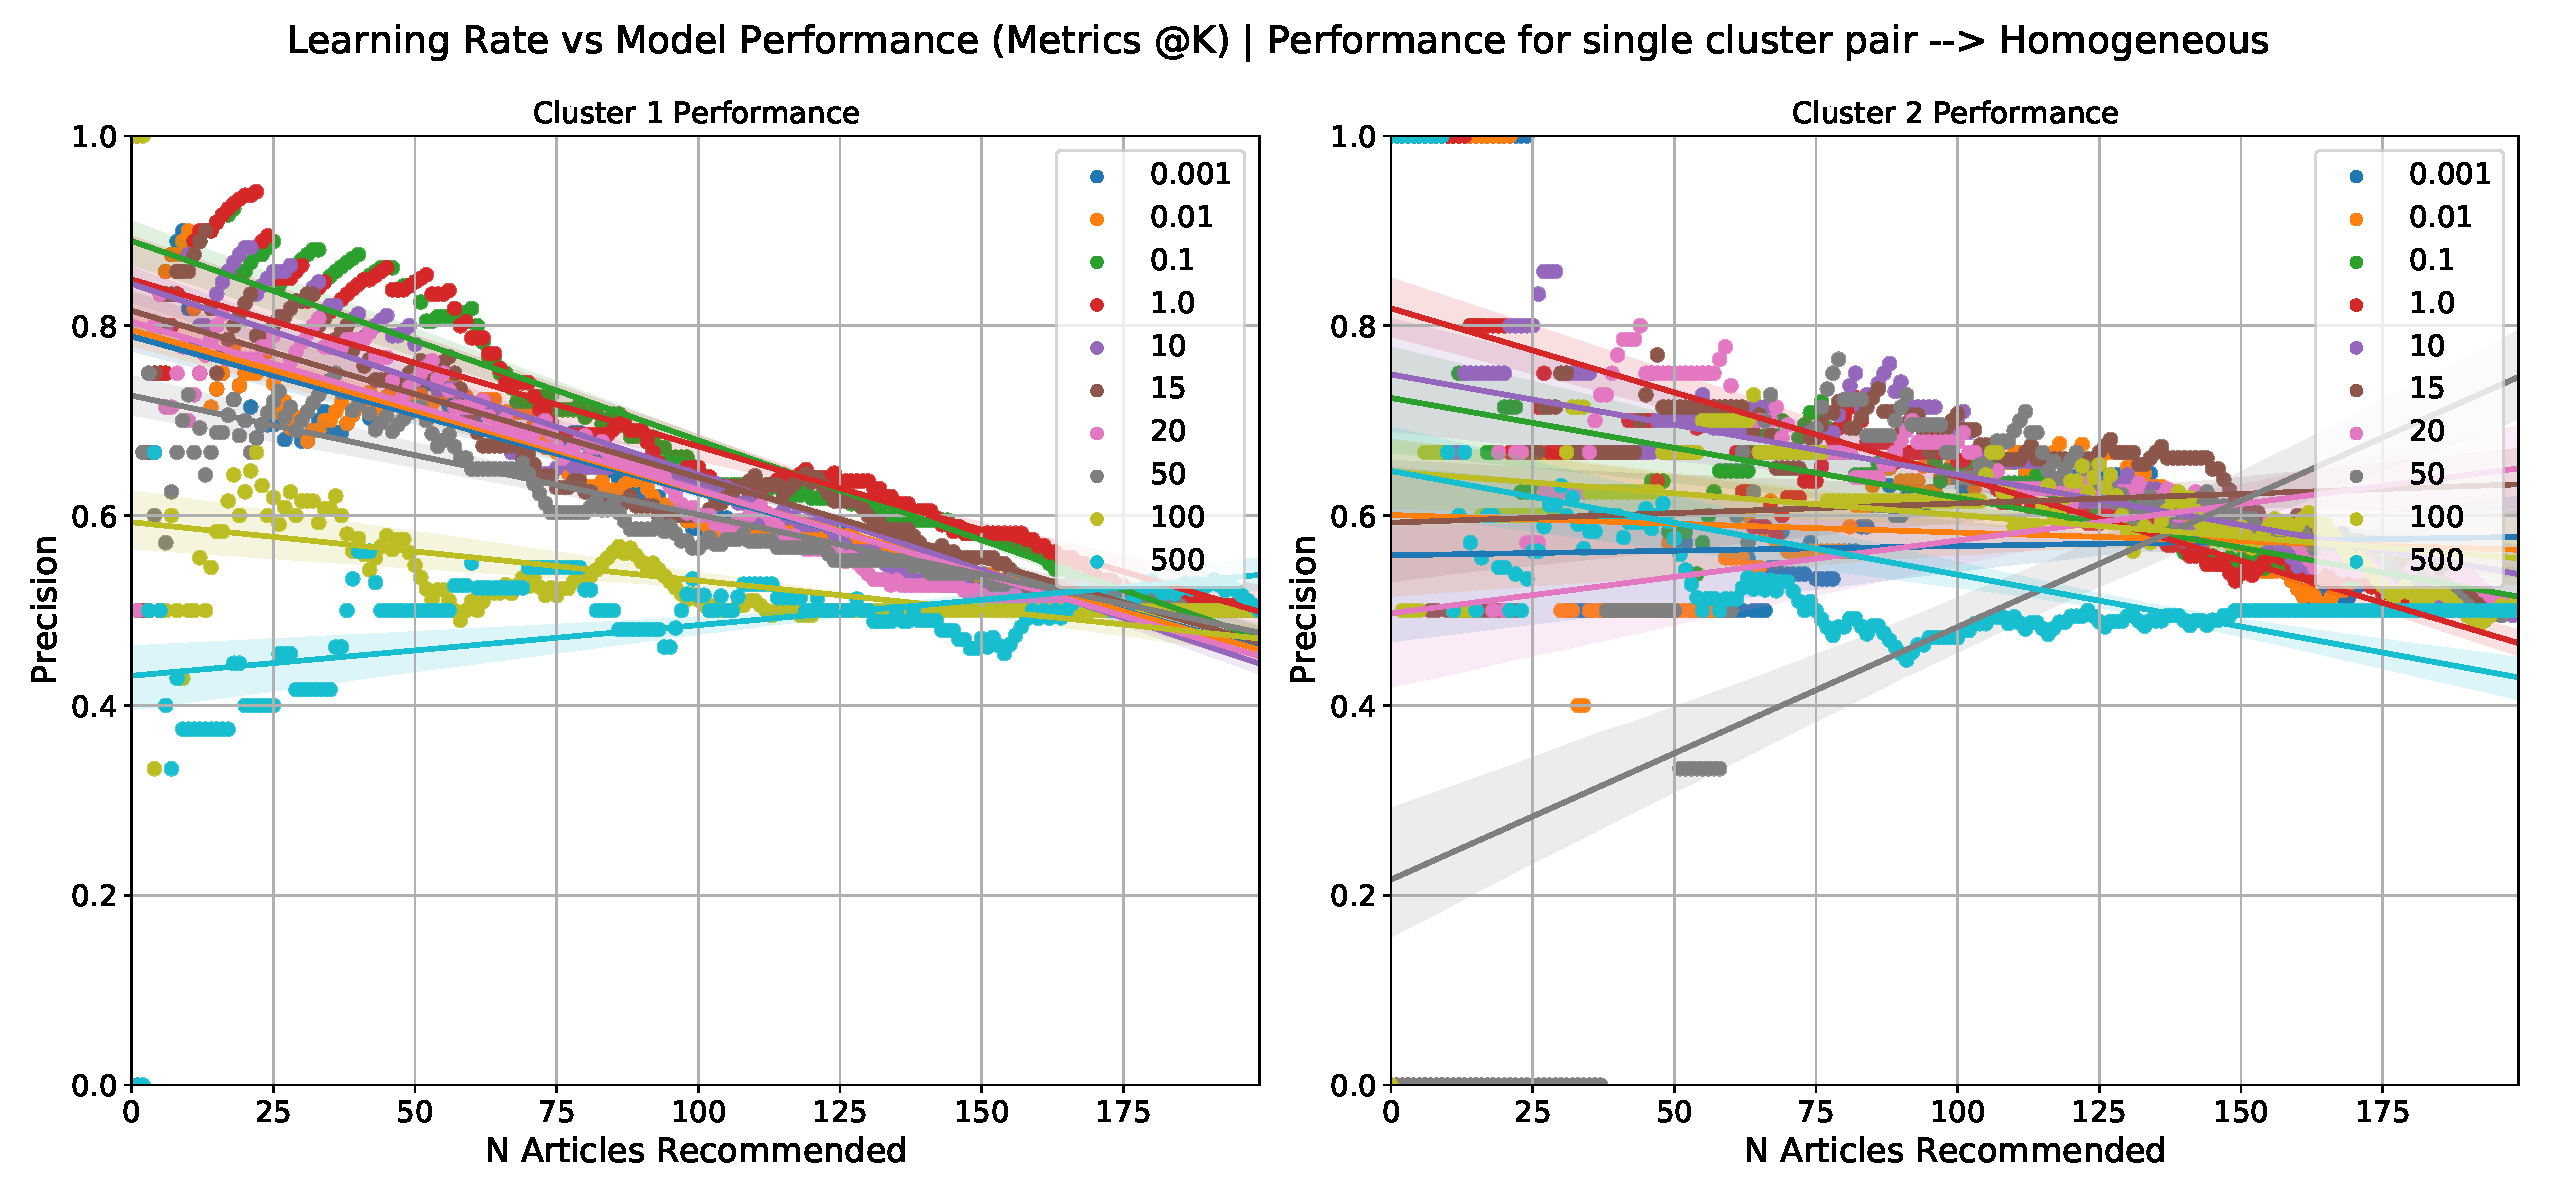
\includegraphics[width=0.7\textwidth]{Graphs/TFIDF/lr_vs_model_performance_single_mixed_Homogeneous.pdf}
    % \caption{Caption}
    % \label{fig:my_label}
\end{figure}
\newpage
\begin{figure}[H]
    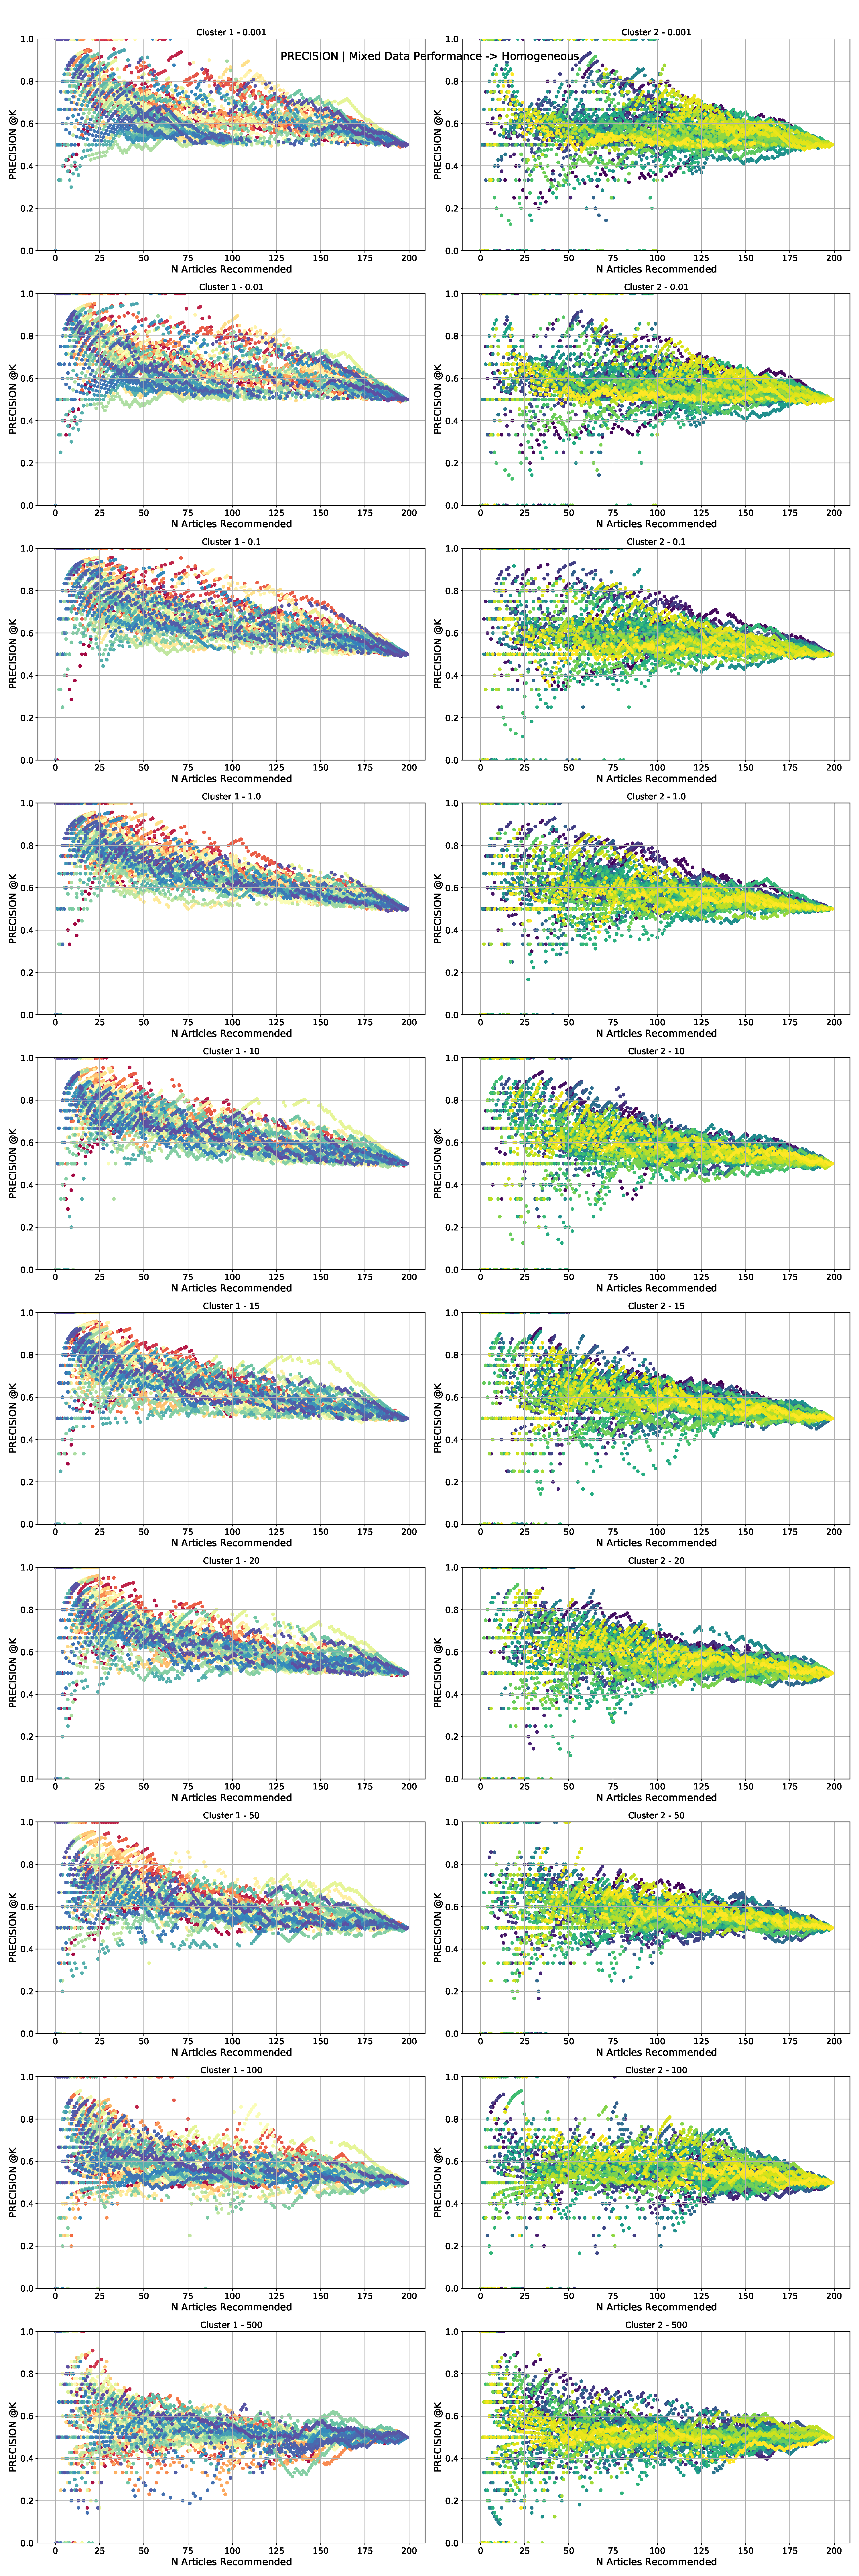
\includegraphics[width=0.5\textwidth]{Graphs/TFIDF/lr_vs_model_performance_precision_all_cps_mixed_data_sep_Homogeneous.pdf}
    % \caption{Caption}
    % \label{fig:my_label}
\end{figure}
\newpage
\subsubsection{Heterogeneous}
\begin{figure}[H]
    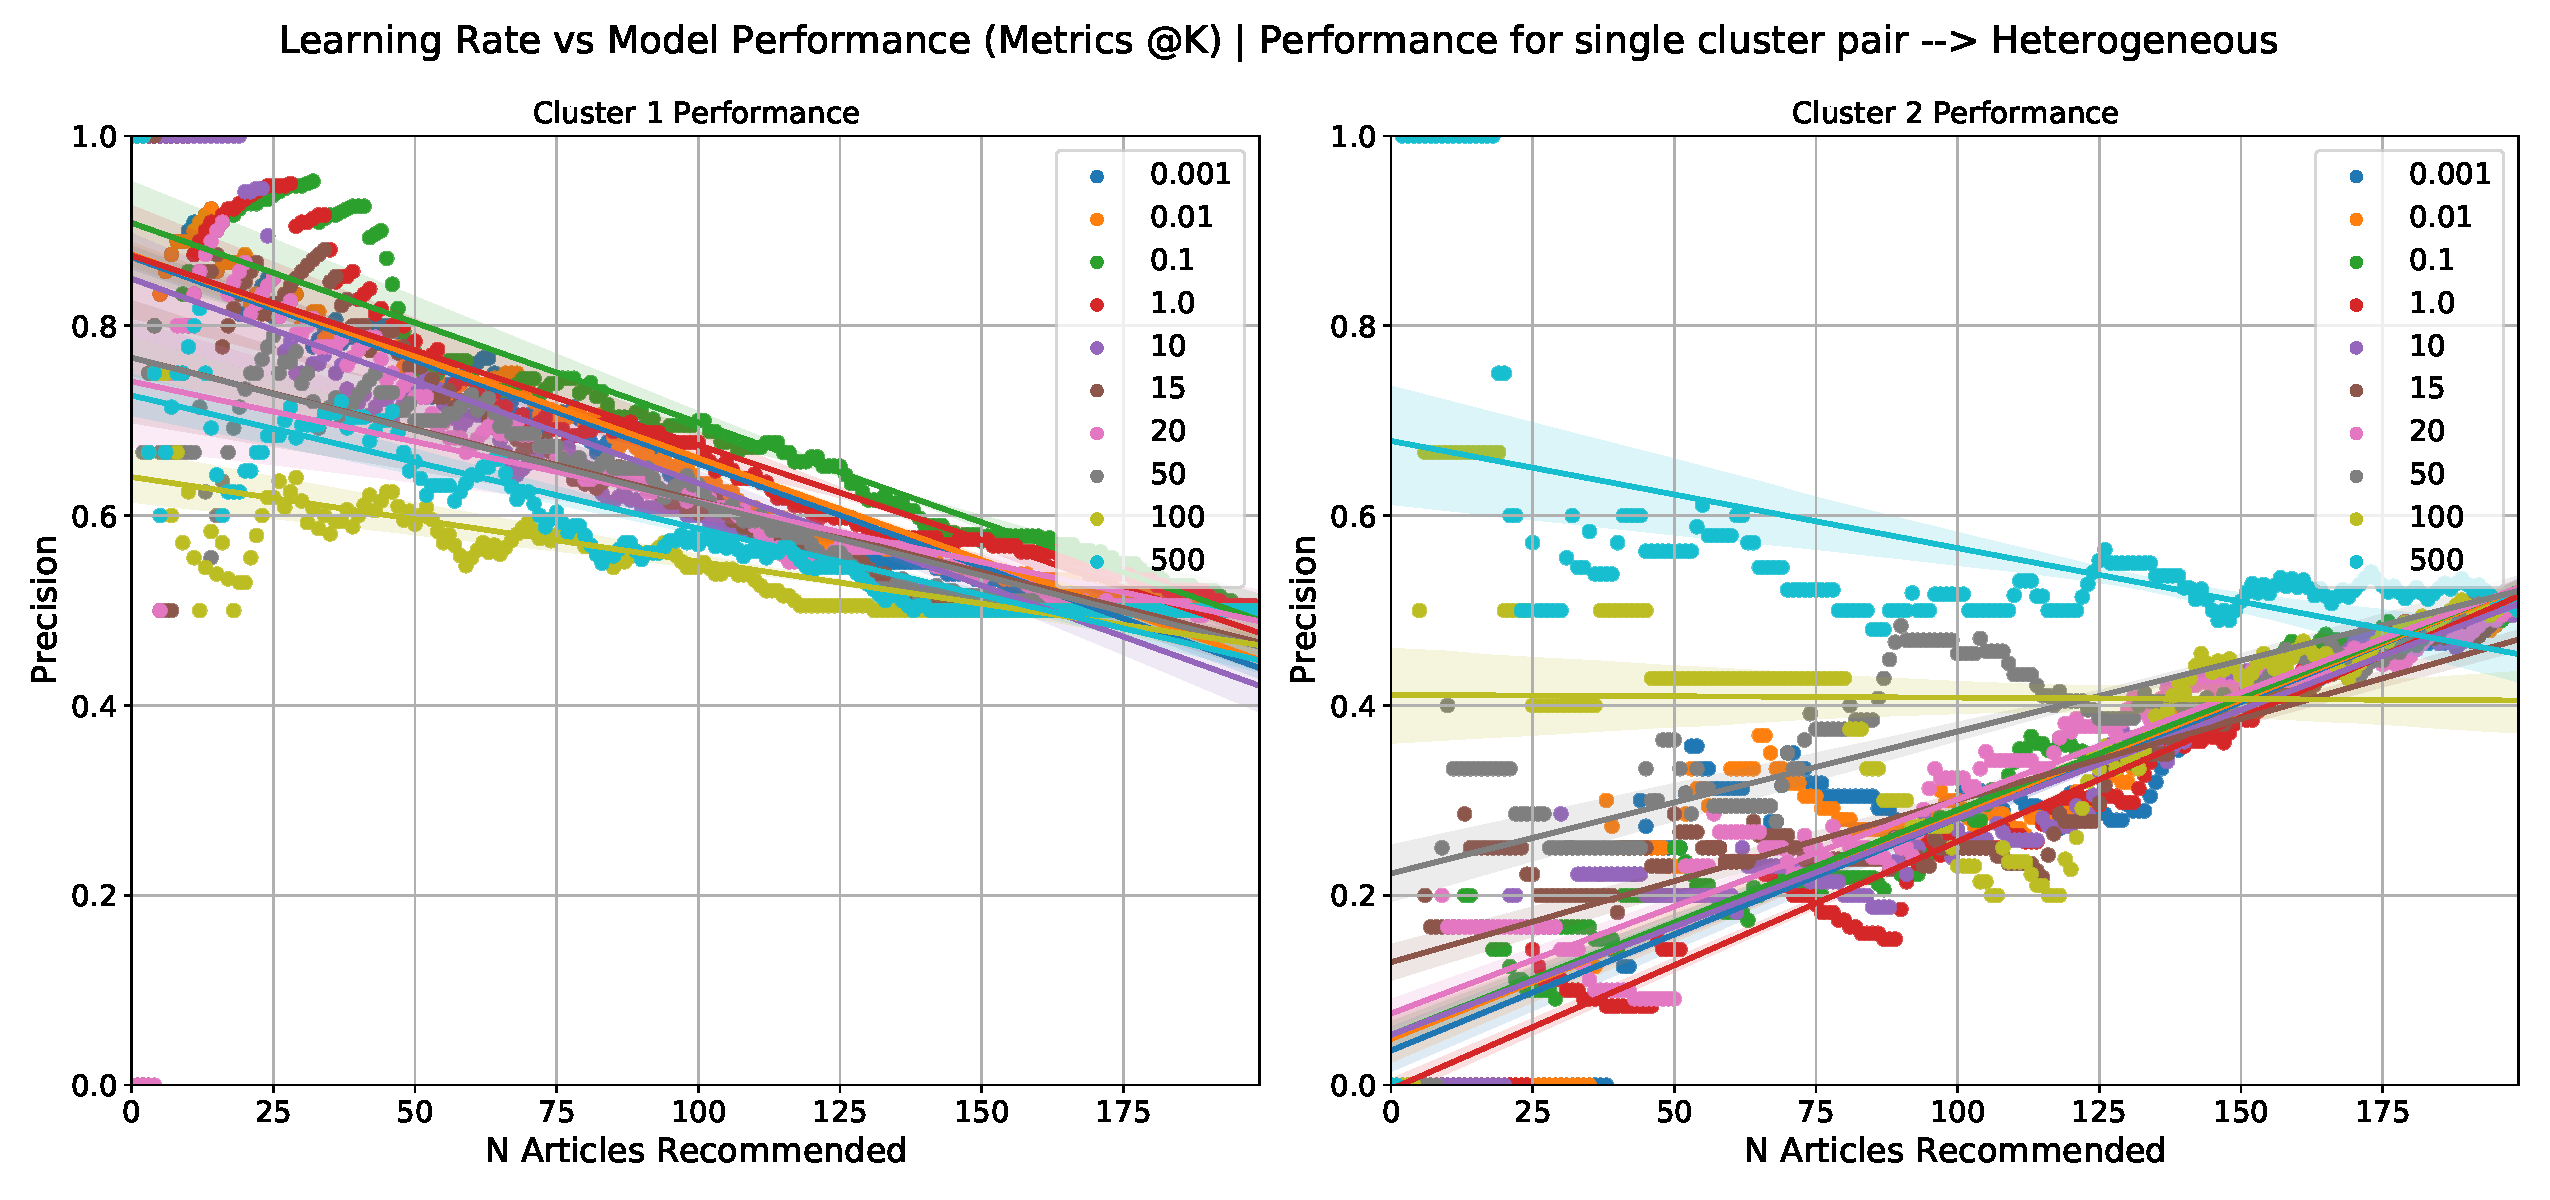
\includegraphics[width=0.7\textwidth]{Graphs/TFIDF/lr_vs_model_performance_single_mixed_Heterogeneous.pdf}
    % \caption{Caption}
    % \label{fig:my_label}
\end{figure}
\newpage
\begin{figure}[H]
    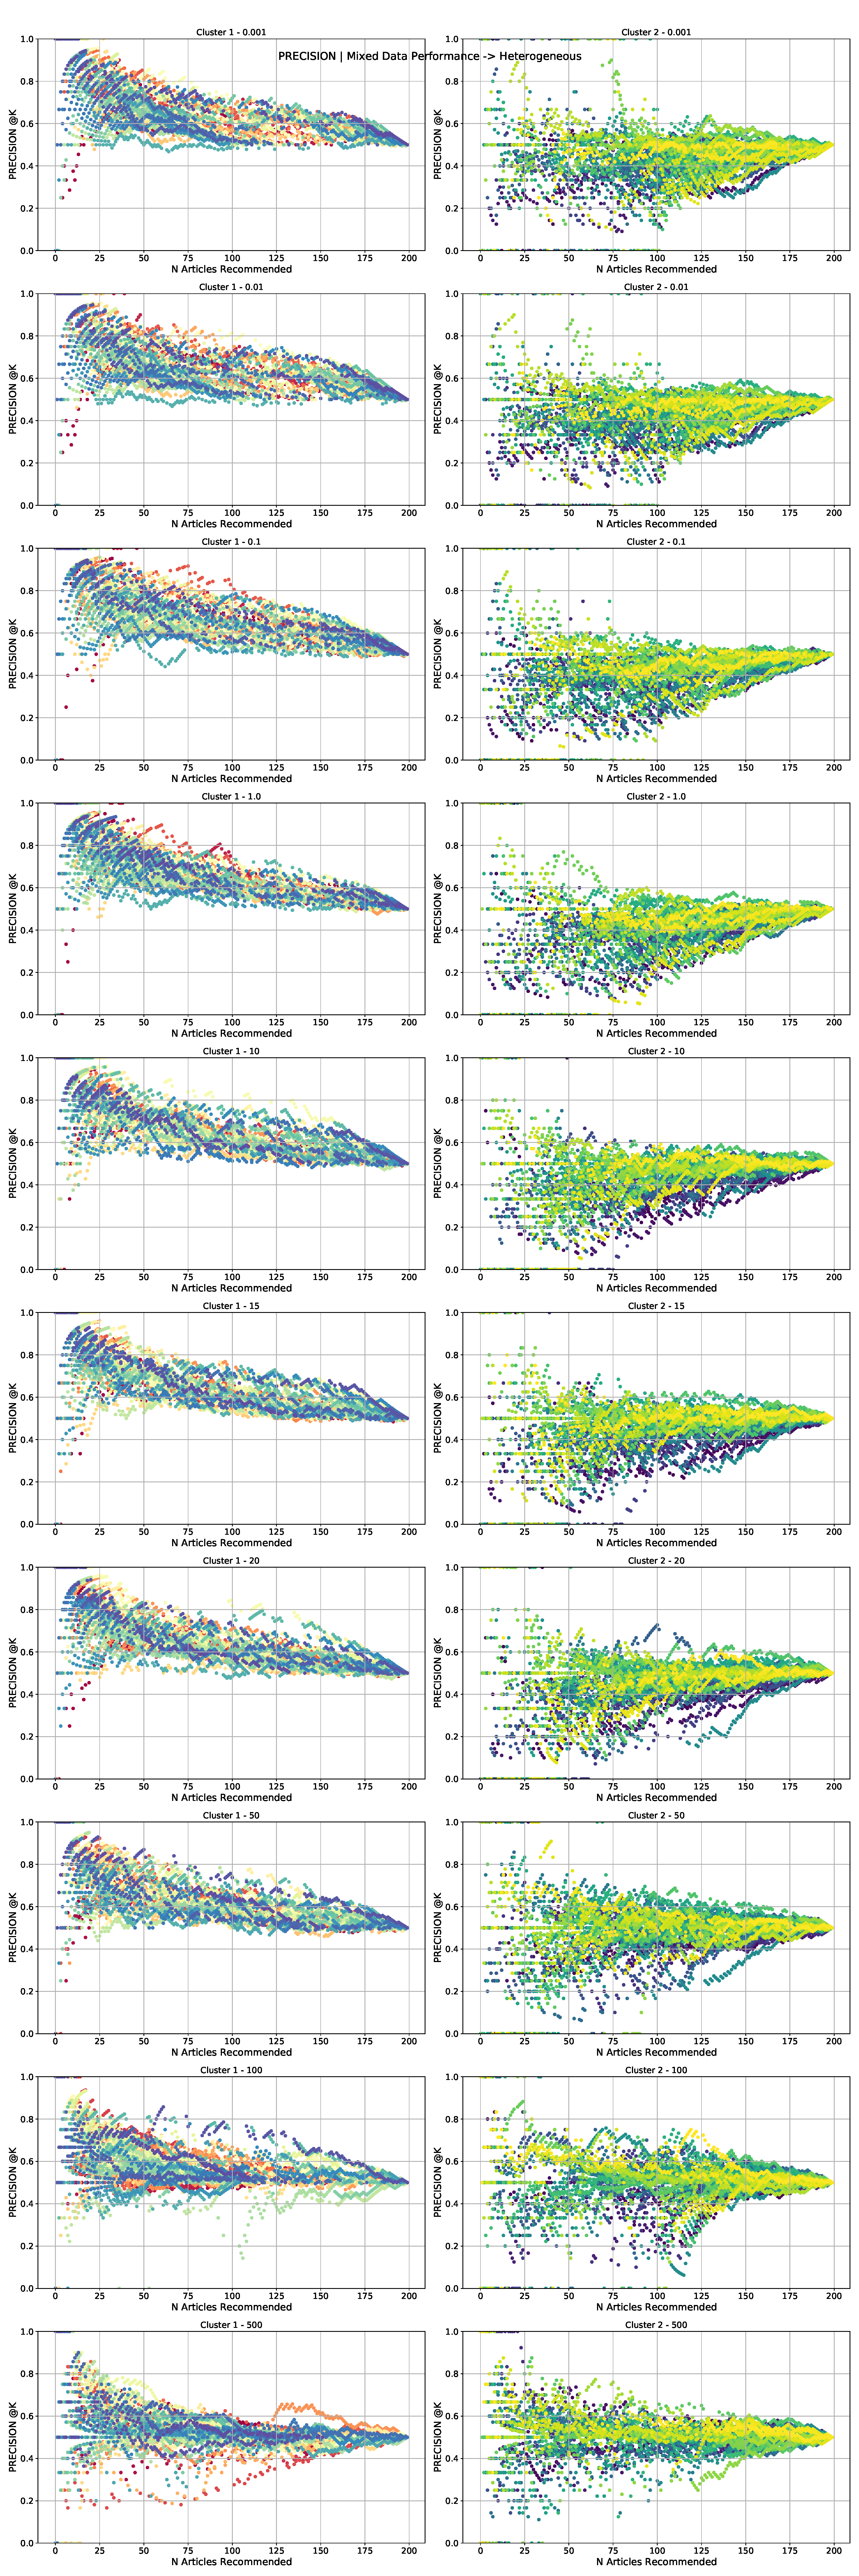
\includegraphics[width=0.5\textwidth]{Graphs/TFIDF/lr_vs_model_performance_precision_all_cps_mixed_data_sep_Heterogeneous.pdf}
    % \caption{Caption}
    % \label{fig:my_label}
\end{figure}
\subsection{Glove}
\subsubsection{Homogeneous}
\begin{figure}[H]
    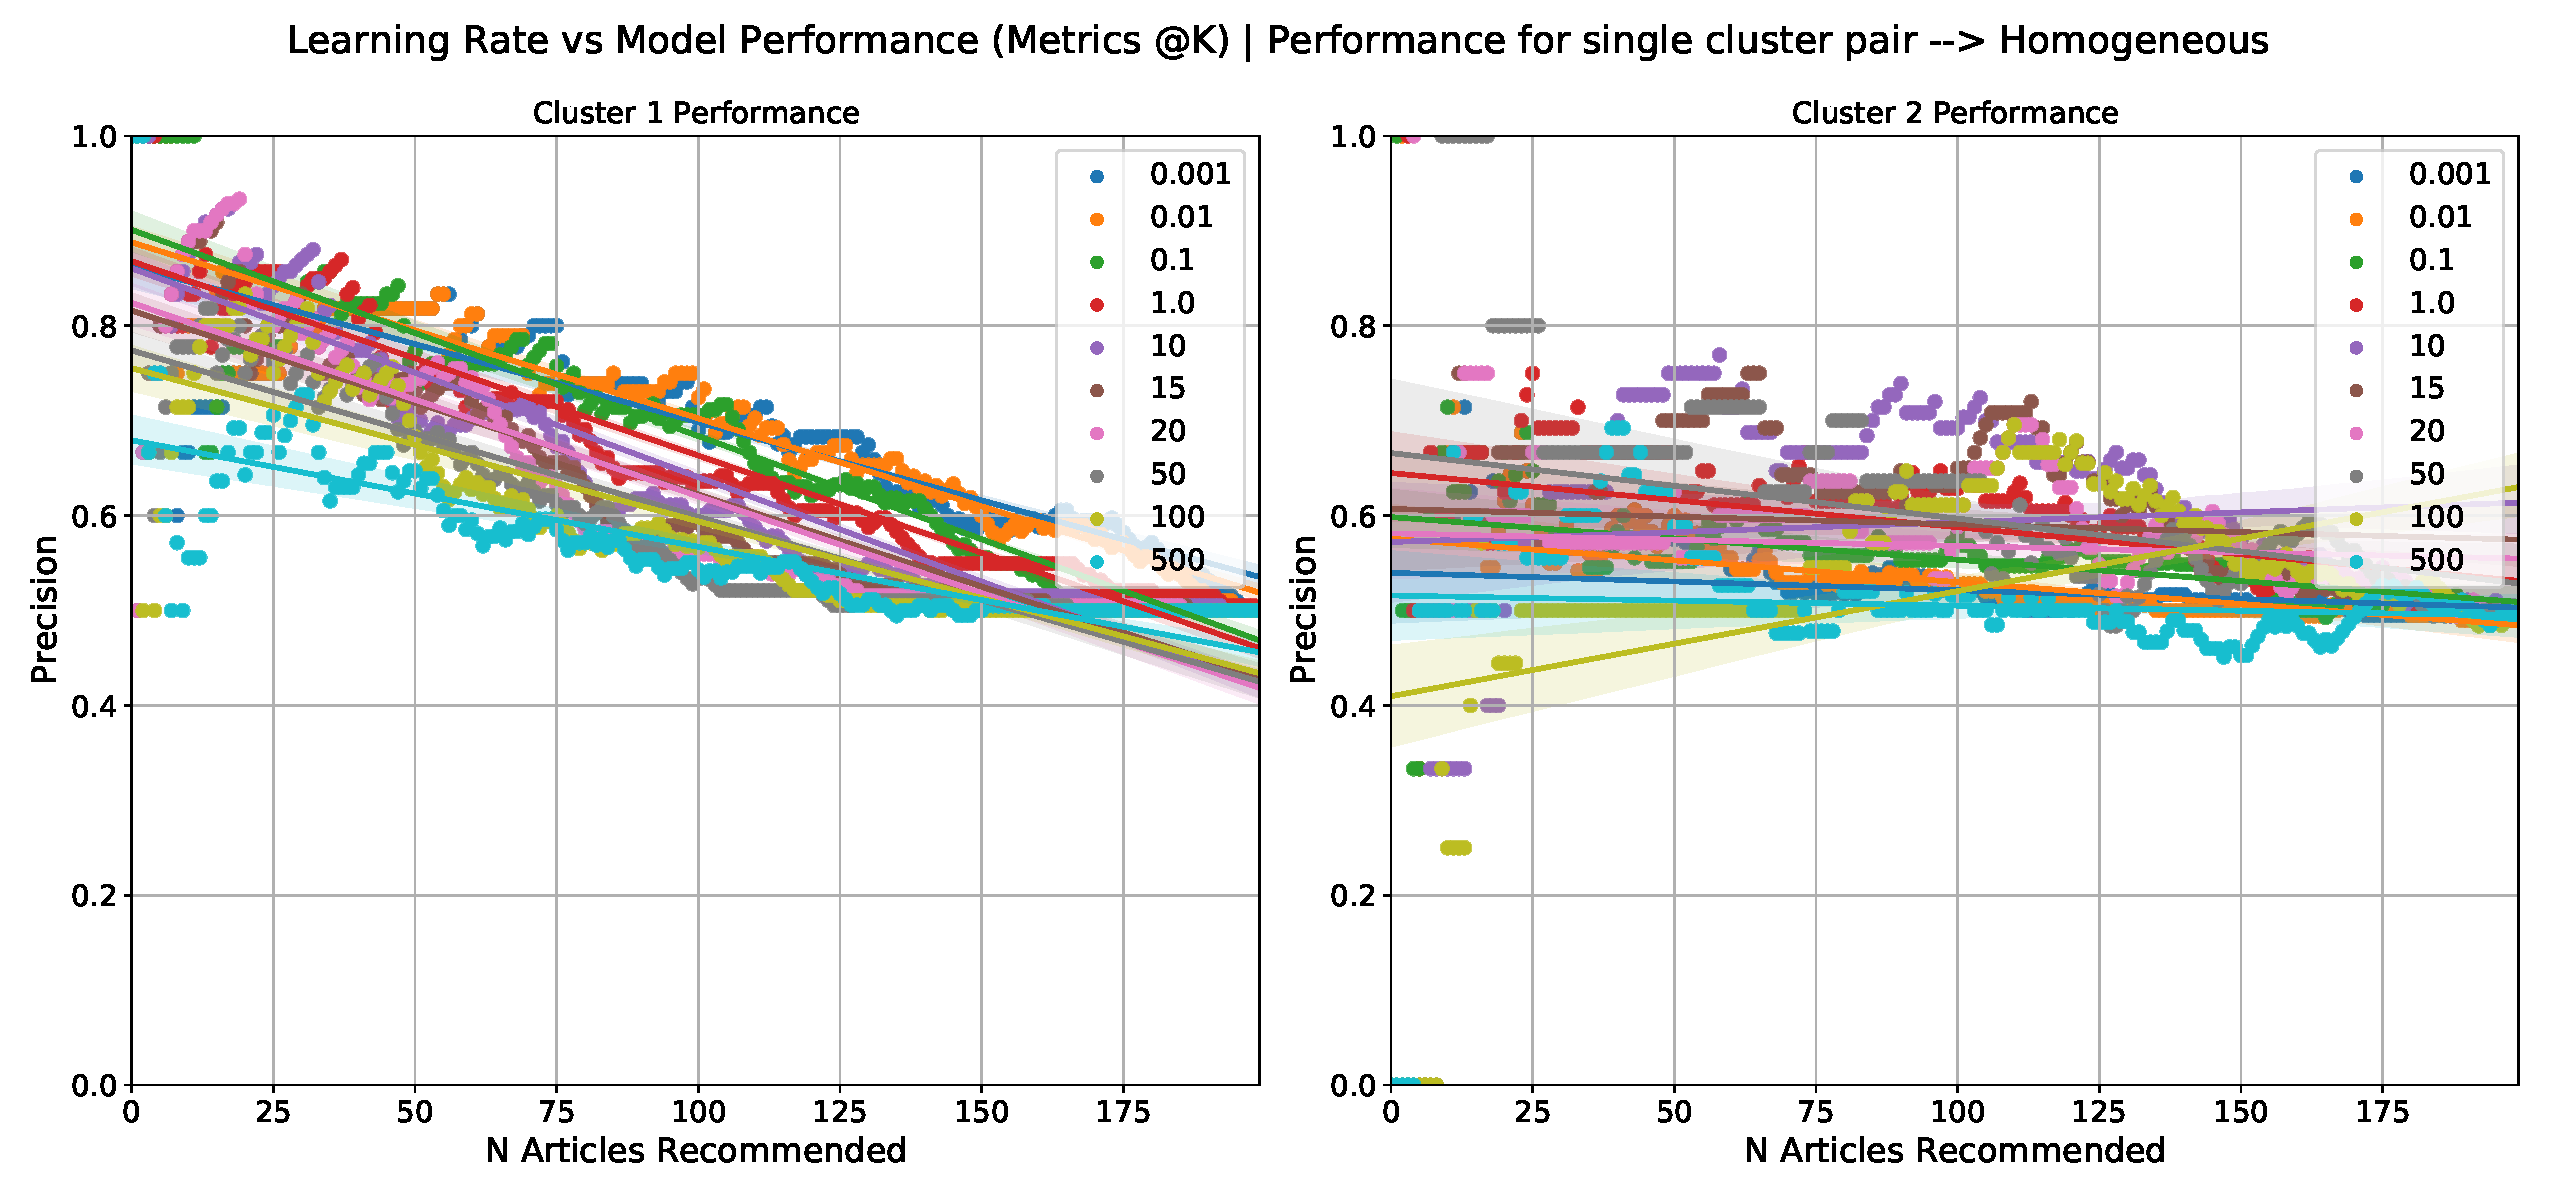
\includegraphics[width=0.7\textwidth]{Graphs/GLOVE/lr_vs_model_performance_single_mixed_Homogeneous.pdf}
    % \caption{Caption}
    % \label{fig:my_label}
\end{figure}
\newpage
\begin{figure}[H]
    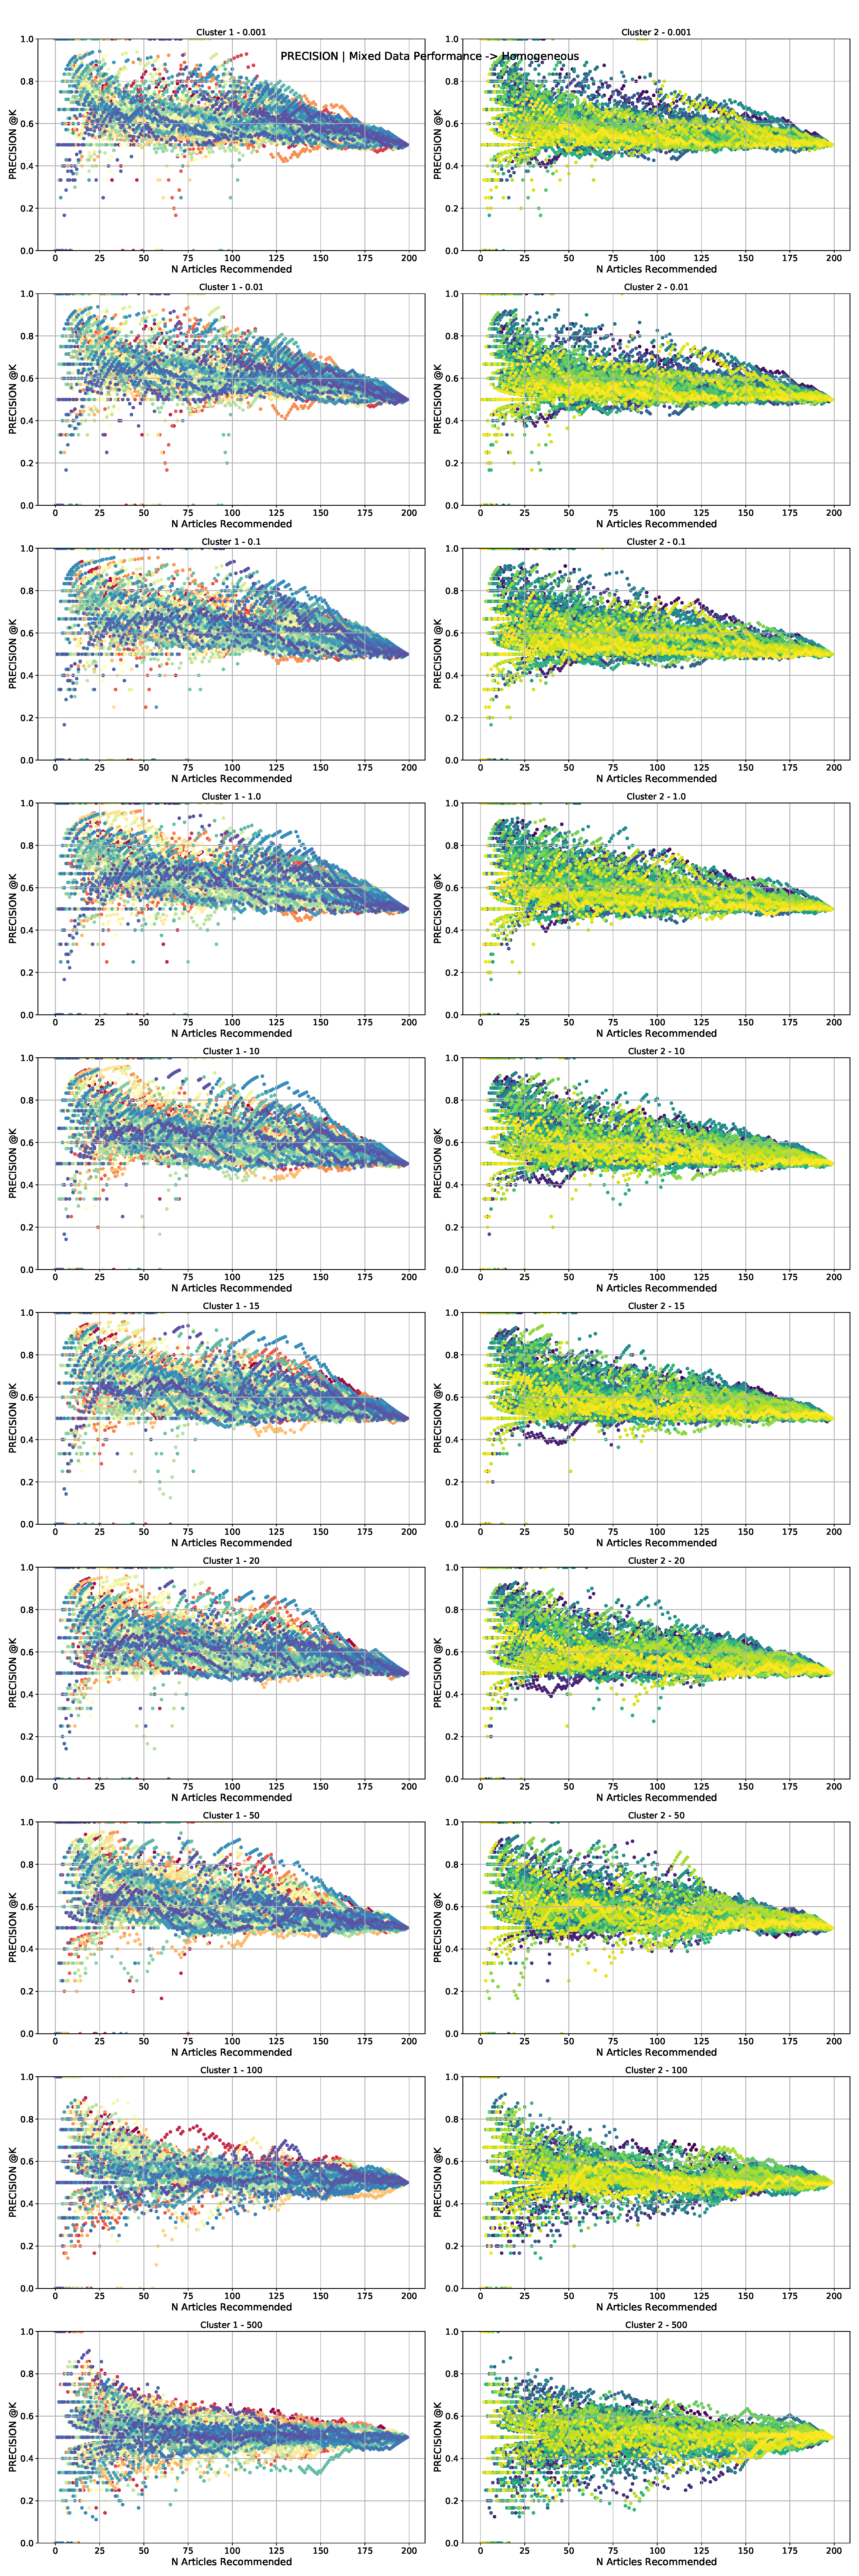
\includegraphics[width=0.5\textwidth]{Graphs/GLOVE/lr_vs_model_performance_precision_all_cps_mixed_data_sep_Homogeneous.pdf}
    % \caption{Caption}
    % \label{fig:my_label}
\end{figure}
\newpage
\subsubsection{Heterogeneous}
\begin{figure}[H]
    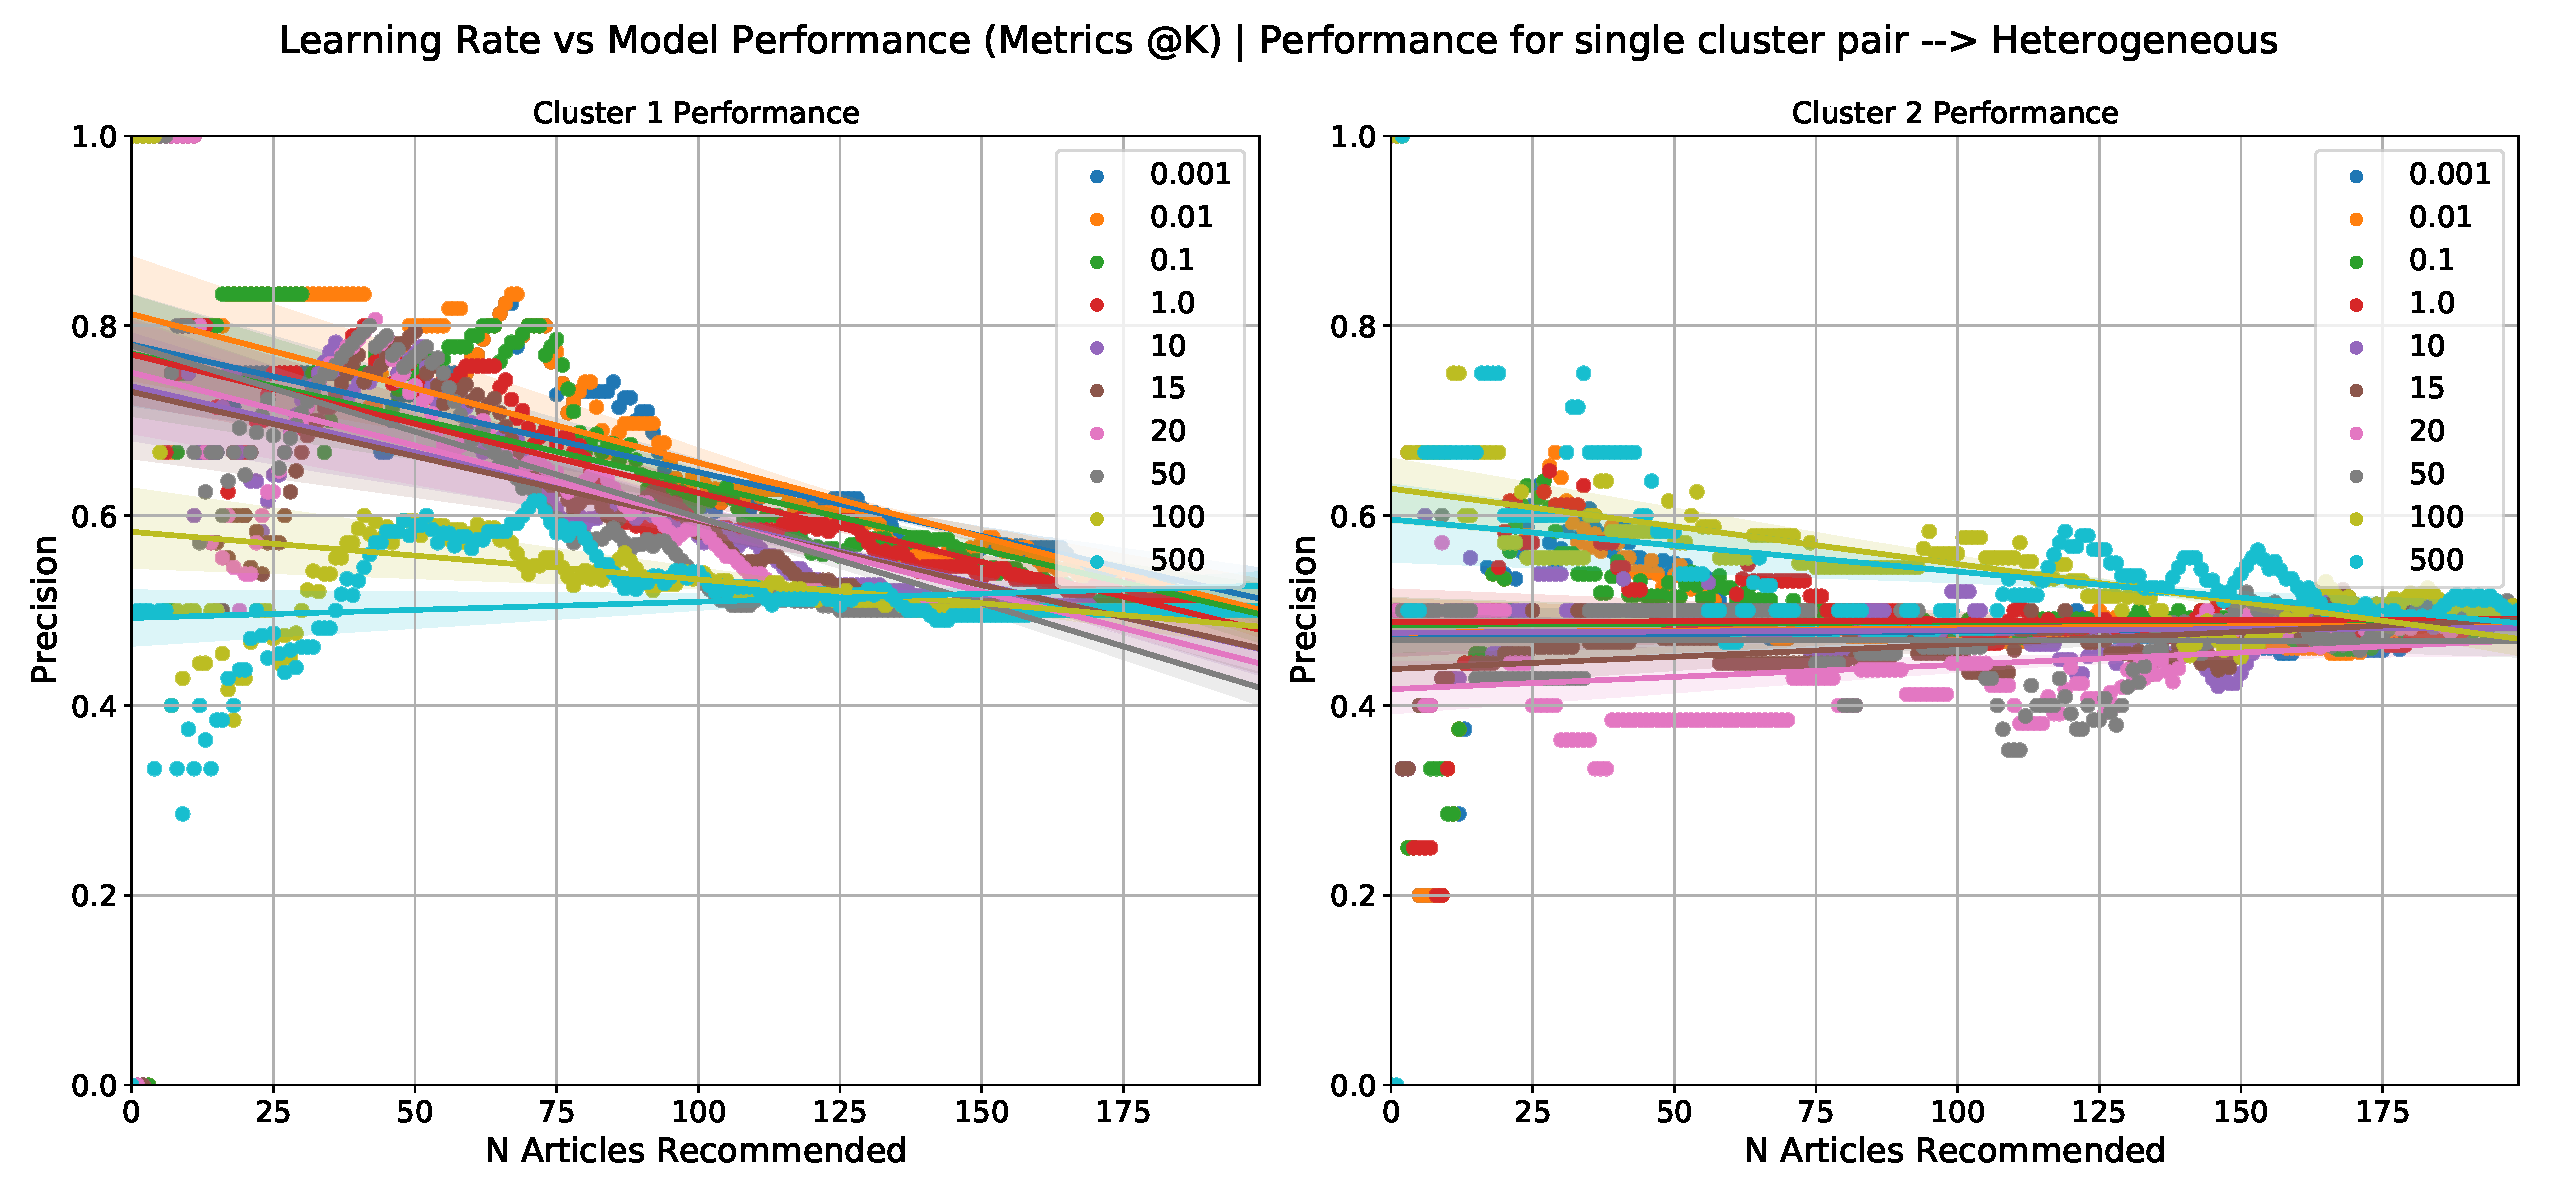
\includegraphics[width=0.7\textwidth]{Graphs/GLOVE/lr_vs_model_performance_single_mixed_Heterogeneous.pdf}
    % \caption{Caption}
    % \label{fig:my_label}
\end{figure}
\newpage
\begin{figure}[H]
    \includegraphics[width=0.5\textwidth]{Graphs/GLOVE/lr_vs_model_performance_precision_all_cps_mixed_data_sep_Heterogeneous.pdf}
    % \caption{Caption}
    % \label{fig:my_label}
\end{figure}
\subsection{BERT}
\subsubsection{Homogeneous}
\begin{figure}[H]
    \includegraphics[width=0.7\textwidth]{Graphs/BERT/lr_vs_model_performance_single_mixed_Homogeneous.pdf}
    % \caption{Caption}
    % \label{fig:my_label}
\end{figure}
\newpage
\begin{figure}[H]
    \includegraphics[width=0.5\textwidth]{Graphs/BERT/lr_vs_model_performance_precision_all_cps_mixed_data_sep_Homogeneous.pdf}
    % \caption{Caption}
    % \label{fig:my_label}
\end{figure}
\newpage
\subsubsection{Heterogeneous}
\begin{figure}[H]
    \includegraphics[width=0.7\textwidth]{Graphs/BERT/lr_vs_model_performance_single_mixed_Heterogeneous.pdf}
    % \caption{Caption}
    % \label{fig:my_label}
\end{figure}
\newpage
\begin{figure}[H]
    \includegraphics[width=0.5\textwidth]{Graphs/BERT/lr_vs_model_performance_precision_all_cps_mixed_data_sep_Heterogeneous.pdf}
    % \caption{Caption}
    % \label{fig:my_label}
\end{figure}



\end{document}